%==============================================================================
%  Multi-Sport Club Management System (MSCMS) -- "Sportify"
%  Graduation Project Report -- main.tex (master skeleton)
%
%  Compiles with pdflatex on Overleaf (no shell-escape, no biber).
%  References use a manual thebibliography (IEEE numeric).
%
%  TEMPLATE NOTE: This layout follows the Menoufia University Faculty of
%  Computers and Information graduation-project template. To re-target the
%  report to another institution, edit the \univName / \facultyName macros
%  in the COVER PAGE block below (search for "EDIT UNIVERSITY HERE").
%==============================================================================

\documentclass[12pt,a4paper]{report}

%------------------------------------------------------------------------------
%  Fonts and encoding (Times-like)
%------------------------------------------------------------------------------
\usepackage[T1]{fontenc}
\usepackage[utf8]{inputenc}
\usepackage{amsmath}             % \tfrac, aligned math, etc.
\usepackage{mathptmx}            % Times-like roman font

%------------------------------------------------------------------------------
%  Page geometry: A4, top/bottom/right = 1in, left = 1.5in
%------------------------------------------------------------------------------
\usepackage[a4paper,top=1in,bottom=1in,left=1.25in,right=1.25in]{geometry}

%------------------------------------------------------------------------------
%  Line spacing: 1.5
%------------------------------------------------------------------------------
\usepackage{setspace}
\onehalfspacing

%------------------------------------------------------------------------------
%  Graphics: screenshots live in screenshots/ (relative to this file)
%------------------------------------------------------------------------------
\usepackage{graphicx}
\graphicspath{{screenshots/}{../screenshots/}{./}}

%------------------------------------------------------------------------------
%  Captions, tables, colour
%------------------------------------------------------------------------------
\usepackage{caption}
\captionsetup{font=small,labelfont=bf,labelsep=period}
\usepackage{booktabs}
\usepackage{longtable}
\usepackage{etoolbox}
\AtBeginEnvironment{longtable}{\setstretch{1}}  % single-space inside tables; avoids split-box infinite-glue warning
\usepackage{array}
\usepackage{tabularx}
\usepackage{multirow}
\usepackage{float}               % [H] exact placement for diagram figures
\usepackage{xcolor}
\usepackage{enumitem}

%  Brand-ish accent colours (used sparingly in listings / rules)
\definecolor{mscmsBlue}{RGB}{0,77,152}
\definecolor{mscmsRed}{RGB}{165,0,52}
\definecolor{codeBg}{RGB}{248,248,248}
\definecolor{codeKw}{RGB}{0,77,152}
\definecolor{codeStr}{RGB}{0,128,0}
\definecolor{codeCmt}{RGB}{120,120,120}
\definecolor{codeFrame}{RGB}{200,200,200}

%------------------------------------------------------------------------------
%  TikZ / UML diagram styles and macros (architecture, use-case, class,
%  ER, state, sequence). Defined in a dedicated file for reuse.
%------------------------------------------------------------------------------
%==============================================================================
%  preamble-diagrams.tex
%  Shared TikZ / UML styling + macros for every diagram in the report.
%  Loaded from main.tex (and from _probe tests) inside the preamble.
%  Diagram types:
%    * Architecture / flowchart / DFD : comp / store / decision / flow styles
%    * Use-case                       : \UCactor , usecase style
%    * Class diagram                  : \UmlClass (rectangle split, 3 parts)
%    * ER diagram                     : \Entity   (rectangle split, 2 parts)
%    * State machine                  : automata library, "st" style
%    * Sequence diagram               : pgf-umlsd (rebranded instances)
%==============================================================================
\usepackage{tikz}
\usepackage{pgf-umlsd}                 % UML sequence diagrams
\usepackage{colortbl}
\usetikzlibrary{positioning,arrows.meta,calc,fit,shapes.geometric,%
                shapes.multipart,backgrounds,automata,shadows.blur,decorations.pathreplacing}

%--- brand palette ------------------------------------------------------------
\definecolor{dBlue}{RGB}{0,77,152}     % Sportify blue
\definecolor{dRed}{RGB}{165,0,52}      % Sportify red
\definecolor{dFill}{RGB}{237,240,252}  % light lavender-blue box fill
\definecolor{dLine}{RGB}{96,112,180}   % box border / connectors
\definecolor{dFill2}{RGB}{233,245,238} % soft green (data stores)
\definecolor{dLine2}{RGB}{70,150,100}

%--- architecture / flowchart / DFD ------------------------------------------
\tikzset{
  comp/.style={rectangle, rounded corners=2pt, draw=dLine, fill=dFill,
               minimum height=9mm, minimum width=24mm, align=center, font=\small},
  svc/.style={comp, fill=dFill, draw=dLine, font=\small\bfseries},
  ext/.style={rectangle, rounded corners=2pt, draw=dRed!70, fill=dRed!6,
              minimum height=9mm, minimum width=24mm, align=center, font=\small},
  store/.style={cylinder, shape border rotate=90, aspect=0.22, draw=dLine2,
                fill=dFill2, minimum height=11mm, minimum width=17mm,
                align=center, font=\scriptsize},
  decision/.style={diamond, aspect=2, draw=dLine, fill=dFill, align=center,
                   font=\scriptsize, inner sep=1pt},
  term/.style={rectangle, rounded corners=4pt, draw=dLine, fill=dFill,
               minimum height=7mm, align=center, font=\scriptsize},
  flow/.style={-{Stealth[length=2.4mm]}, draw=dLine, thick},
  flowd/.style={-{Stealth[length=2.4mm]}, draw=dLine, thick, dashed},
  biflow/.style={{Stealth[length=2.4mm]}-{Stealth[length=2.4mm]}, draw=dLine, thick},
  lbl/.style={font=\scriptsize, fill=white, inner sep=1pt},
}

%--- state machine ------------------------------------------------------------
\tikzset{
  st/.style={circle, draw=dLine, fill=dFill, minimum size=13mm,
             font=\scriptsize, align=center, inner sep=0pt},
  stbox/.style={rectangle, rounded corners=3pt, draw=dLine, fill=dFill,
                minimum size=10mm, font=\scriptsize, align=center},
}

%--- class diagram : \UmlClass[pos]{node}{Name}{attributes}{methods} ----------
\tikzset{
  cls/.style={draw=dLine, fill=white, rounded corners=1pt,
              rectangle split, rectangle split parts=3,
              rectangle split part fill={dFill,white,white},
              inner sep=3pt, align=left, font=\scriptsize, text width=36mm},
  clshead/.style={cls},
}
\newcommand{\UmlClass}[5][]{%
  \node[cls,#1] (#2) {\textbf{#3}\nodepart{two}#4\nodepart{three}#5};}

%--- ER diagram : \Entity[pos]{node}{TITLE}{rows} -----------------------------
\tikzset{
  ent/.style={draw=dLine, fill=white, rounded corners=1pt,
              rectangle split, rectangle split parts=2,
              rectangle split part fill={dFill,white},
              inner sep=3pt, align=left, font=\scriptsize, text width=33mm},
}
\newcommand{\Entity}[4][]{%
  \node[ent,#1] (#2) {\textbf{#3}\nodepart{two}#4};}
% relationship connector with two multiplicity labels and a verb
\newcommand{\Rel}[5]{% {from}{to}{nearlabel}{farlabel}{verb}
  \draw[dLine] (#1) -- node[lbl,pos=0.12]{#3} node[lbl,pos=0.5]{\itshape #5}
       node[lbl,pos=0.88]{#4} (#2);}

%--- use-case -----------------------------------------------------------------
\tikzset{
  actorpic/.pic={
    \draw[dLine,thick] (0,0) circle (2.4mm);
    \draw[dLine,thick] (0,-2.4mm) -- (0,-10mm);
    \draw[dLine,thick] (-4.5mm,-5.5mm) -- (4.5mm,-5.5mm);
    \draw[dLine,thick] (0,-10mm) -- (-3.5mm,-16mm);
    \draw[dLine,thick] (0,-10mm) -- (3.5mm,-16mm);},
  usecase/.style={ellipse, draw=dLine, fill=dFill, align=center,
                  font=\scriptsize, minimum width=28mm, minimum height=9mm,
                  inner sep=1pt},
}
% \UCactor{x}{y}{label}  -- places a stick actor with a caption underneath
\newcommand{\UCactor}[3]{\pic at (#1,#2) {actorpic};
  \node[font=\scriptsize\bfseries] at ($(#1,#2)-(0,2.1)$){#3};}

%--- rebrand pgf-umlsd instances/threads to the palette -----------------------
\tikzset{inststyle/.style={rectangle, draw=dLine, fill=dFill, rounded corners=1pt,
        anchor=west, minimum height=0.8cm, minimum width=1.8cm}}
\tikzset{threadstyle/.style={rectangle, draw=dLine, fill=dFill, rounded corners=1pt,
        anchor=west, minimum height=0.8cm, minimum width=1.8cm}}

%--- a light helper for figure sizing -----------------------------------------
\newcommand{\diagcap}[2]{\caption{#1}\label{#2}}


%------------------------------------------------------------------------------
%  Source-code listings (Java / JavaScript / Bash)
%------------------------------------------------------------------------------
\usepackage{listings}
\lstset{
  basicstyle=\ttfamily\footnotesize,
  backgroundcolor=\color{codeBg},
  keywordstyle=\color{codeKw}\bfseries,
  stringstyle=\color{codeStr},
  commentstyle=\color{codeCmt}\itshape,
  numberstyle=\tiny\color{codeCmt},
  frame=single,
  rulecolor=\color{codeFrame},
  breaklines=true,
  breakatwhitespace=true,
  showstringspaces=false,
  tabsize=2,
  captionpos=b,
  numbers=left,
  numbersep=6pt,
  xleftmargin=14pt,
  framexleftmargin=14pt,
  columns=fullflexible,
  keepspaces=true
}

% Convenience language aliases used by the chapter files.
\lstdefinelanguage{JavaScriptES}{
  keywords={break,case,catch,const,continue,default,delete,do,else,export,
            extends,finally,for,function,if,import,in,instanceof,let,new,
            return,super,switch,this,throw,try,typeof,var,void,while,with,
            yield,async,await,of,class},
  morecomment=[l]{//},
  morecomment=[s]{/*}{*/},
  morestring=[b]',
  morestring=[b]",
  morestring=[b]`,
  sensitive=true
}
\lstdefinelanguage{bashx}{
  keywords={cd,echo,export,docker,compose,mvn,java,curl,git,npm,run,build,up,down},
  morecomment=[l]{\#},
  morestring=[b]',
  morestring=[b]",
  sensitive=true
}

%------------------------------------------------------------------------------
%  Hyperlinks (no coloured boxes)
%------------------------------------------------------------------------------
\usepackage[hidelinks,breaklinks=true]{hyperref}
\hypersetup{
  pdftitle={Multi-Sport Club Management System (MSCMS) -- Sportify},
  pdfauthor={MSCMS Team},
  pdfsubject={Graduation Project Report},
  pdfkeywords={microservices, Spring Boot, Next.js, Keycloak, sports management}
}

%------------------------------------------------------------------------------
%  Headers / footers: footer page numbers, light chapter header
%------------------------------------------------------------------------------
\usepackage{lastpage}            % total page count for "Page N of M"
\usepackage{fancyhdr}
\pagestyle{fancy}
\fancyhf{}
\renewcommand{\headrulewidth}{0pt}
\renewcommand{\footrulewidth}{0pt}
\fancyfoot[L]{\small Page~\textbf{\thepage}~of~\pageref{LastPage}}

% Plain style (chapter-opening pages) carries the same footer.
\fancypagestyle{plain}{%
  \fancyhf{}%
  \renewcommand{\headrulewidth}{0pt}%
  \fancyfoot[L]{\small Page~\textbf{\thepage}~of~\pageref{LastPage}}%
}

%------------------------------------------------------------------------------
%  Decorative double-rule border drawn on every page (learnova style).
%------------------------------------------------------------------------------
\usepackage{eso-pic}
\AddToShipoutPictureBG{%
  \begin{tikzpicture}[overlay,remember picture]
    \draw[line width=1.4pt]
      ([shift={( 1.05cm,-1.05cm)}]current page.north west) rectangle
      ([shift={(-1.05cm, 1.05cm)}]current page.south east);
    \draw[line width=0.5pt]
      ([shift={( 1.20cm,-1.20cm)}]current page.north west) rectangle
      ([shift={(-1.20cm, 1.20cm)}]current page.south east);
  \end{tikzpicture}}

%------------------------------------------------------------------------------
%  Spacing helpers
%------------------------------------------------------------------------------
%------------------------------------------------------------------------------
%  Chapter headings: numbered chapters get a learnova-style DIVIDER PAGE
%  (title alone, vertically centred on its own page); unnumbered front-matter
%  chapters (Acknowledgment, Summary, References) keep a normal top heading.
%------------------------------------------------------------------------------
\makeatletter
\renewcommand{\@makechapterhead}[1]{%
  \vspace*{\fill}%
  {\parindent\z@ \centering \normalfont
    {\Huge\bfseries\color{mscmsBlue}\@chapapp\ \thechapter}\par\nobreak
    \vskip 28\p@
    {\Huge\bfseries #1}\par\nobreak}%
  \vspace*{\fill}%
  \clearpage}
\renewcommand{\@makeschapterhead}[1]{%
  \vspace*{6\p@}%
  {\parindent\z@ \normalfont
    {\Huge\bfseries\color{mscmsBlue} #1}\par\nobreak
    \vskip 22\p@}}
\makeatother

\setlength{\parskip}{0.4em}
\setlength{\parindent}{1.5em}

%==============================================================================
%  EDIT UNIVERSITY HERE -- change these two macros to re-target the institution.
%  The previous report used Menoufia University; the placeholder below keeps the
%  university name editable while defaulting to the Menoufia layout.
%==============================================================================
\newcommand{\univName}{Menoufia University}      % <-- {University Name}
\newcommand{\facultyName}{Faculty of Computers and Information}
\newcommand{\projectYear}{2025 -- 2026}          % <-- academic year
\newcommand{\submissionDate}{June 2026}

\begin{document}

%==============================================================================
%  COVER PAGE
%==============================================================================
\pagenumbering{arabic}           % single arabic sequence, cover = page 1 (learnova)
\thispagestyle{fancy}
{\setlength{\parskip}{0pt}%
\begin{center}

% --- University / faculty banner: two crests flanking the institution name ----
\noindent
\begin{minipage}[c]{0.22\textwidth}\centering
  \IfFileExists{screenshots/fci-logo.png}{
\includegraphics[height=2.2cm]{fci-logo.png}}{}
\end{minipage}\hfill
\begin{minipage}[c]{0.52\textwidth}\centering
  {\Large\bfseries \univName \par}\vspace{4pt}
  {\large\bfseries \facultyName \par}
\end{minipage}\hfill
\begin{minipage}[c]{0.22\textwidth}\centering
  \IfFileExists{screenshots/menoufia-logo.png}{
\includegraphics[height=2.2cm]{menoufia-logo.png}}{}
\end{minipage}

\vspace{1.1cm}

% --- Title --------------------------------------------------------------------
{\Huge\bfseries\color{mscmsBlue} Multi-Sport Club Management System \par}
\vspace{0.35cm}
{\LARGE\bfseries (MSCMS) \par}

\vspace{0.8cm}

{\Large\itshape A Cloud-Native Microservices Platform \par}
\vspace{0.15cm}
{\Large\itshape for Modern Sports Club Operations \par}

\vspace{0.6cm}
{\huge\bfseries\color{mscmsRed} Sportify \par}

\vspace{1.0cm}
\rule{0.6\textwidth}{0.4pt}
\vspace{0.7cm}

% --- Team members -------------------------------------------------------------
{\large\bfseries Submitted by \par}
\vspace{0.3cm}
{\large
\begin{tabular}{c}
Mariam Mohamed Ahmed \\[2pt]
Mohamed Abdellatief \\[2pt]
Eman Ahmed Elboghdady \\[2pt]
Khaled Mohamed \\[2pt]
Shahd Abdelaziz \\[2pt]
Mohamed Salem \\
\end{tabular}\par}

\vspace{0.8cm}

% --- Supervisor ---------------------------------------------------------------
{\large\bfseries Supervised by: Dr. Shaimaa Saber \par}

\vspace{0.9cm}

% --- Footer -------------------------------------------------------------------
{\normalsize A graduation project submitted in partial fulfilment of the \par}
{\normalsize requirements for the degree of B.Sc.\ in Computer Science \par}
\vspace{0.5cm}
{\Large\bfseries \projectYear \par}

\end{center}}
\clearpage

%==============================================================================
%  FRONT MATTER (continuous arabic numbering, learnova style)
%==============================================================================

%------------------------------------------------------------------------------
%  Acknowledgment
%------------------------------------------------------------------------------
\chapter*{Acknowledgment}
\addcontentsline{toc}{chapter}{Acknowledgment}
\markboth{Acknowledgment}{Acknowledgment}

First and foremost, the team expresses its sincere gratitude to its supervisor,
\textbf{Dr.~Shaimaa Saber}, whose continuous guidance, technical insight and
encouragement shaped this project from an initial idea into a complete,
production-grade platform. Her thoughtful feedback at every milestone, and her
patience throughout the long iterations of design and implementation, were
invaluable to the work presented in this report.

The team is also deeply grateful to the staff of the \facultyName{} at
\univName{} for providing the academic environment, laboratories and curriculum
that made this work possible. Special thanks are due to the instructors of the
software-engineering, databases and distributed-systems courses, whose teaching
laid the conceptual foundations on which the Multi-Sport Club Management System
(MSCMS) was built.

Finally, the team thanks its families and friends for their unwavering support,
patience and motivation throughout the many months of design, development and
testing. This project is the product of their collective encouragement as much
as of the team's own effort.

\vspace{1cm}
\noindent\textit{The MSCMS Team, \submissionDate.}

%------------------------------------------------------------------------------
%  Summary / Abstract
%------------------------------------------------------------------------------
\chapter*{Summary}
\addcontentsline{toc}{chapter}{Summary}
\markboth{Summary}{Summary}

The \textbf{Multi-Sport Club Management System (MSCMS)}, delivered under the
product brand \textbf{Sportify}, is a cloud-native, microservices-based platform
that unifies every operational concern of a modern multi-sport club into a
single, role-aware web application. Taking the real organisational structure of
FC~Barcelona as its working model, the system consolidates user and team
administration, player and squad operations, training, match operations, medical
and fitness management, scouting, sponsorship, analytics and fan engagement that
are traditionally scattered across spreadsheets, e-mail threads and disconnected
tools.

The back-end is built as a set of Spring~Boot~3.5.6 / Java~21 microservices
coordinated by Spring~Cloud: a Eureka discovery server, a centralised Config
Server, and a single API Gateway that performs JWT verification and routing.
Identity is delegated to Keycloak, each domain service owns its own PostgreSQL
database, and asynchronous events flow over Apache~Kafka, with Redis caching and
RabbitMQ available for messaging. The front-end is a Next.js~16 / React~19
application styled with Tailwind~CSS~v4, enforcing the same role-based access
control rules as the gateway. The entire stack is containerised with Docker and
orchestrated through Docker Compose.

This report documents the project's full lifecycle and, in particular, the
substantial enhancements delivered since the previous milestone. Key capabilities
of the platform include:

\begin{itemize}[leftmargin=1.6em,itemsep=2pt]
  \item \textbf{Cloud-native microservices architecture} -- seven Spring~Boot
        services behind a Eureka/Config/Gateway control plane, each independently
        deployable and backed by its own database.
  \item \textbf{Centralised identity and expert RBAC} -- Keycloak-issued JWTs
        and a fine-grained, per-role page-access map enforced at both the gateway
        and the Next.js middleware.
  \item \textbf{Database-backed Competitions} -- a real La~Liga season and the
        new-format UEFA Champions League (single league phase plus a knockout
        bracket), with completed competitions automatically locked read-only.
  \item \textbf{Real match ingestion} -- scheduled synchronisation of fixtures
        and standings from football-data.org, with the back-end as the single
        source of truth.
  \item \textbf{Live-match engine} -- a broadcast-style phase machine (first and
        second half, stoppage time, and extra time plus penalties for knockout
        ties only), with lineups locked at creation, per-sport substitution
        limits and in-match injury events.
  \item \textbf{Medical injury-management workflow} -- a Treatment Room that
        separates currently-injured from recovered players and tracks each player
        through a staged journey from injury to diagnosis, treatment,
        rehabilitation, recovery and fitness testing.
  \item \textbf{Real-time team messaging} -- a group-chat system with group
        invitations and emoji reactions delivered over a WebSocket channel with a
        polling fallback.
  \item \textbf{Event-driven notifications and alerts} -- a top-bar notification
        bell fed by Kafka-sourced events and live-match alerts.
  \item \textbf{Persistent settings} -- profile, preference and notification
        settings with real persistence and a Keycloak-verified password change.
  \item \textbf{Sportify rebrand} -- a unified, club-themed visual identity across
        the entire front-end.
\end{itemize}

The result is a scalable, observable and secure system that demonstrates how a
microservices architecture, a central identity provider and event-driven
integration can resolve the data fragmentation, multi-discipline complexity and
analytical blindness that characterise traditional club-management tooling.

%------------------------------------------------------------------------------
%  Tables of contents / figures / tables
%------------------------------------------------------------------------------
\cleardoublepage
\tableofcontents

\cleardoublepage
\addcontentsline{toc}{chapter}{List of Figures}
\listoffigures

\cleardoublepage
\addcontentsline{toc}{chapter}{List of Tables}
\listoftables

%------------------------------------------------------------------------------
%  Abbreviations
%------------------------------------------------------------------------------
\cleardoublepage
\chapter*{List of Abbreviations}
\addcontentsline{toc}{chapter}{List of Abbreviations}
\markboth{List of Abbreviations}{List of Abbreviations}

\renewcommand{\arraystretch}{1.3}
\begin{longtable}{p{0.20\textwidth} p{0.74\textwidth}}
\toprule
\textbf{Abbreviation} & \textbf{Meaning} \\
\midrule
\endfirsthead
\toprule
\textbf{Abbreviation} & \textbf{Meaning} \\
\midrule
\endhead
\bottomrule
\endlastfoot
MSCMS   & Multi-Sport Club Management System \\
API     & Application Programming Interface \\
REST    & Representational State Transfer \\
JWT     & JSON Web Token \\
RBAC    & Role-Based Access Control \\
ER      & Entity--Relationship \\
UML     & Unified Modeling Language \\
CRUD    & Create, Read, Update, Delete \\
HTTP    & Hypertext Transfer Protocol \\
HTTPS   & Hypertext Transfer Protocol Secure \\
JSON    & JavaScript Object Notation \\
SQL     & Structured Query Language \\
RDBMS   & Relational Database Management System \\
IdP     & Identity Provider \\
OAuth   & Open Authorization \\
OIDC    & OpenID Connect \\
SPA     & Single-Page Application \\
SSR     & Server-Side Rendering \\
UI      & User Interface \\
UX      & User Experience \\
CL      & UEFA Champions League \\
PD      & Primera Divisi\'on (La~Liga) competition code \\
WC      & FIFA World Cup competition code \\
XI      & Starting Eleven (match lineup) \\
KPI     & Key Performance Indicator \\
ML      & Machine Learning \\
WS      & WebSocket \\
DTO     & Data Transfer Object \\
JPA     & Java Persistence API \\
DB      & Database \\
CI/CD   & Continuous Integration / Continuous Delivery \\
TLS     & Transport Layer Security \\
UUID    & Universally Unique Identifier \\
CORS    & Cross-Origin Resource Sharing \\
\end{longtable}
\renewcommand{\arraystretch}{1.0}

%==============================================================================
%  BODY (continuous arabic numbering)
%==============================================================================

\chapter{Introduction}
\label{ch:introduction}

\section{Context}
\label{sec:context}

Contemporary sports clubs have evolved into complex, data-intensive organisations whose
day-to-day operations bear little resemblance to the amateur structures of previous
decades. A modern professional club is no longer a single team supported by a coach and a
physiotherapist; it is a multi-discipline enterprise that simultaneously fields teams across
several sports, employs dozens of specialised staff, manages hundreds of contracted
athletes, and engages a global audience of supporters. Each of these activities continuously
generates operational data: training sessions and the load they impose, match fixtures and
the events that unfold within them, medical incidents and the rehabilitation journeys that
follow, scouting assessments of prospective signings, sponsorship negotiations, contract
renewals, and the constant stream of communication that binds these functions together.
A club of this kind is, in effect, a small enterprise whose product is sporting performance
and whose raw material is information: who is fit, who is in form, who the next opponent is,
what the medical staff have advised, and what the commercial department has agreed.

To appreciate why the management of this information has become a first-order engineering
problem, it is useful to situate the present work within the broader sports-technology
landscape. Over the past two decades the discipline now widely referred to as
\emph{sports analytics} has matured from a niche curiosity into a mainstream competitive
advantage. Professional clubs routinely instrument their athletes with wearable sensors that
sample heart rate, acceleration and positional data hundreds of times per second; they
record and tag every match with frame-accurate video; and they purchase event-level data
feeds that describe every pass, shot and tackle in a fixture. The volume and velocity of this
data have grown to the point where it can no longer be managed by hand, and the clubs that
extract value from it are precisely those that have invested in the software infrastructure to
collect, integrate and reason over it. Sport, in other words, has become a software-intensive
domain, and the quality of a club's information systems is now a genuine determinant of its
performance both on and off the field.

This transformation has been mirrored on the supporter side. Consumer-facing data
platforms such as SofaScore and ESPN have reset public expectations about how sporting
information should be presented: fixtures, results, league standings and minute-by-minute
event timelines are now expected to be available instantly, updated live as matches unfold,
and rendered through polished, responsive interfaces on any device. A supporter who can
watch a match update second-by-second on a free mobile application will not tolerate a club
portal that displays last week's results entered by hand. The bar for immediacy, breadth and
presentation has been set by the consumer web, and any platform that a club exposes to its
own staff and supporters is implicitly measured against it.

The working setting for this project is the multi-sport club model exemplified by
FC~Barcelona, an organisation that operates several professional teams under a single
governing body while sharing common medical, scouting, analytics and commercial
departments. This setting was chosen deliberately because it captures the full breadth of
the problem: the same governing entity must reason about distinct sports, each with its own
positions, formations, competition calendars and performance indicators, while still
enforcing a single coherent identity, a unified access-control policy and a shared analytical
backbone. A platform that can serve such an organisation must therefore be genuinely
multi-tenant across disciplines, role-aware down to the level of individual job functions, and
capable of ingesting and presenting real competition data rather than merely storing
hand-entered records. The multi-sport club is not an arbitrary stress test; it is the natural
habitat of the very fragmentation problem this project sets out to solve, because every
shared department---medical, scouting, analytics, commercial---must serve teams whose
sporting logic differs while still drawing on one common pool of people, contracts and money.

The technical context is equally important. The systems that successfully manage data at
this scale in other industries---banking, logistics, e-commerce---have converged on a
common architectural style: rather than a single large program, they are built as a federation
of small, independently deployable services, each owning a well-defined slice of the domain
and its data, communicating over network protocols, and coordinated by shared
infrastructure for discovery, configuration and routing. This \emph{cloud-native
microservices} style~\cite{microservices} is not a fashion but a response to a concrete set of
pressures that a multi-sport club exhibits in full: heterogeneous domains that evolve at
different rates, the need to isolate failures so that an outage in one area does not take down
the whole organisation, and the desirability of scaling read-heavy public surfaces
independently of write-heavy internal tooling. The live-match engine, for example, is a
bursty, real-time workload that behaves nothing like the steady, transactional load of the
medical records subsystem, and forcing both into a single deployable unit would mean that
neither could be tuned, scaled or released on its own terms.

In practice, the data that should knit these activities together is instead scattered across
disconnected spreadsheets, third-party SaaS subscriptions, e-mail threads and printed
forms. A player's injury record maintained by the medical department is invisible to the
coach planning the next training block; a scout's report on a prospect never reaches the
sport manager negotiating the transfer in a structured form; and a supporter following the
club has no window onto the same fixtures, results and squad information that the club
itself maintains internally. The cost of this fragmentation is not merely inconvenience: it is
duplicated effort, reconciliation errors, stale information driving real decisions, and the
practical impossibility of asking cross-domain questions---such as whether a particular
training regime correlates with a rise in soft-tissue injuries, or whether a scout's
recommendations have historically panned out. This fragmentation is the central motivation
for the \emph{Multi-Sport Club Management System} (MSCMS), delivered under the product
brand \emph{Sportify}: a single, cloud-native platform that consolidates the operational
concerns of a multi-sport club and exposes each of them through one consistent, secured
interface, while adopting the real-time, data-rich presentation philosophy that the
consumer web has made the baseline expectation.

\section{Motivation}
\label{sec:motivation}

The motivation behind MSCMS is to consolidate every operational concern of a multi-sport
club into one cohesive platform, in which each professional role is presented only with the
information relevant to its responsibilities, and in which every data point is traceable,
secured and analytically meaningful. The design draws directly on the real organisational
structure of a large European club: a single governing body managing multiple professional
teams across several sports, supported by shared medical, scouting, analytics and
sponsorship functions. Modelling a real club rather than an abstract one forces the system
to confront the genuine complexity of multi-discipline operation instead of solving an
artificially simplified problem. Concretely, the platform models a catalogue of fourteen
distinct professional roles---administrator, head coach, assistant coach, specific coach,
fitness coach, performance analyst, team doctor, physiotherapist, team manager, sport
manager, scout, sponsor, player and supporter---each of which sees a different slice of the
system. Designing for fourteen roles rather than the three or four that generic team tools
assume is itself a forcing function: it exposes exactly the access-control, navigation and
data-ownership questions that a real club must answer and that simpler products are free to
ignore.

A second, equally important motivation is the desire to move beyond static record-keeping
towards a living, real-time platform. Earlier generations of club-management software
treated data as something to be entered after the fact: a fixture was recorded once it had
been played, an injury was logged once treatment had begun. The expectations of modern
staff and supporters, shaped by data-rich consumer platforms such as SofaScore and ESPN,
are very different. Users now expect matches to update live, notifications to arrive the
moment an event occurs, and dashboards to reflect the current state of the club rather than
yesterday's. MSCMS is therefore motivated not only by the goal of unifying fragmented
data, but by the goal of doing so in a manner that is real-time, event-driven and
operationally trustworthy. This ambition manifests in three concrete capabilities that recur
throughout this report: a live-match engine that drives a fixture through its phases as it is
actually played, recording goals, substitutions and injuries against a phase-bounded clock;
an event-driven notification fabric in which a significant occurrence in one domain
automatically surfaces an alert in another, without the two domains being directly coupled;
and a real-time team chat that lets staff coordinate over a persistent connection. Each of
these is real-time not as a veneer but as a structural property of the architecture.

A third motivation is correctness and trustworthiness of data. For a system to serve as a
single source of truth, it is not enough to gather data in one place; the data must be
internally consistent and protected against both accidental corruption and unauthorised
disclosure. This motivates two design commitments that shape much of the system. The first
is that the backend, not the browser or any external feed, is the authoritative source for
every fact the platform presents: when real competition data is ingested from an external
provider it is normalised and stored internally, and the front-end reads only from the
backend, so that there is exactly one version of the truth and one place to audit it. The
second is that sensitive operations are guarded consistently: medical and financial data are
visible only to the roles entitled to see them, and a destructive or irreversible action---such
as changing a password---is verified against the identity provider before it is allowed to
proceed. Trust, in a system that a club would actually rely on, is not a feature bolted on at
the end; it is a property that must be designed in from the data model outward.

Finally, the project is motivated by sound engineering practice. A platform of this breadth,
spanning identity, squad management, competitions, live matches, medical workflows,
messaging, notifications and analytics, cannot reasonably be built or maintained as a single
monolithic application. The motivation to adopt a cloud-native microservices
architecture~\cite{microservices} arises directly from the need for independent
deployability, fault isolation between domains, and the ability to evolve one functional area
(for example the live-match engine) without destabilising another (for example the medical
records subsystem). Decomposing the system along domain boundaries also yields a clean
mapping between the organisational structure of the club and the structure of the
software---squad operations, competitions and matches, medical and fitness, analytics and
reporting, and communication each become their own service with their own database---which
makes the system easier to reason about, to test in isolation, and to assign to different
developers working in parallel. The choice of Spring Boot~\cite{springboot} for the backend,
the Spring Cloud~\cite{springcloud} ecosystem for the discovery, configuration and gateway
control plane, and a RESTful inter-service contract~\cite{restapi} complemented by
asynchronous events follows naturally from this motivation.

\section{Scope}
\label{sec:scope}

The scope of MSCMS spans the principal operational domains of a multi-sport club, each
realised as a coherent feature area within the platform:

\begin{enumerate}
  \item \textbf{Identity and Role Management} --- centralised authentication through a
        self-hosted identity provider~\cite{keycloak} issuing signed JSON Web
        Tokens~\cite{jwt}, with a rich catalogue of fourteen professional roles organised
        into permission tiers and enforced uniformly across the system at three layers: the
        identity provider, the API gateway, and the front-end route guards~\cite{rbac}.
  \item \textbf{Squad and Club Operations} --- player and staff rosters, player profiles
        with photographs and detailed attributes, contracts, transfers and call-ups, and a
        dedicated Club Hub presenting the club's identity, squad, trophy cabinet and recent
        form.
  \item \textbf{Competitions} --- database-backed competitions covering a domestic league
        (La~Liga, modelled as a double round-robin) and the newly formatted UEFA
        Champions League (a single thirty-six-team league phase generated algorithmically,
        followed by a two-legged knockout bracket), with standings, fixtures and results
        recomputed and presented per competition, and completed competitions automatically
        locked read-only.
  \item \textbf{Match Operations} --- fixture creation with a mandatory starting line-up
        locked at creation, a live-match engine that drives a match through its phases in
        real time and automatically goes live at the exact scheduled kickoff, in-match event
        recording bounded by the current phase, per-sport substitution limits, and read-only
        match details for completed fixtures.
  \item \textbf{Medical and Fitness} --- a structured injury-management workflow that
        carries each affected player through a staged recovery journey---injury, diagnosis,
        treatment, rehabilitation, recovery and fitness testing---driven by the injury status
        as a single source of truth, alongside general medical catalogues, organised within a
        dedicated Treatment Room view that separates currently-injured from recovered
        players.
  \item \textbf{Communication} --- real-time team group chat with group membership,
        invitations that must be accepted, and message reactions, delivered over a persistent
        WebSocket connection~\cite{websocket} with a polling fallback.
  \item \textbf{Notifications and Alerts} --- an event-driven notification fabric, fed by a
        message broker~\cite{kafka}, that surfaces role-aware, priority-tagged alerts through
        an in-application notification centre reachable from a top-bar bell.
  \item \textbf{Reports, Analytics and Machine Learning} --- aggregated dashboards,
        downloadable reports, scouting and sponsorship workflows, and decoupled
        machine-learning services for match-outcome prediction and player-rating estimation,
        consumed transparently through the interface.
\end{enumerate}

The scope explicitly includes the ingestion of real competition data~\cite{footballdata} so
that competitions, fixtures and results reflect genuine football rather than synthetic
placeholders, and it includes a fan-facing surface so that supporters can follow the club
through the same platform the club uses internally. The scope deliberately excludes building
a bespoke identity provider, a custom message broker or a proprietary data feed; instead the
system integrates mature, well-understood components for these concerns and concentrates
its engineering effort on the club-management domain itself. Equally, the scope is bounded to
the football discipline for competitions and live matches---the domain in which authoritative
external data is available---while the role model, squad operations and medical workflows are
designed to generalise across sports. The boundaries of the system are drawn so that the
project demonstrates depth in the domains it claims rather than shallow breadth across
domains it cannot fully support.

\section{Problem Definition}
\label{sec:problem}

A modern multi-sport club faces a constellation of operational problems that no single
off-the-shelf product addresses end-to-end:

\begin{itemize}
  \item \textbf{Fragmented data across departments.} Medical, coaching, scouting,
        analytics and commercial functions each maintain isolated spreadsheets, documents
        and SaaS subscriptions. A player's injury record is invisible to the coach planning
        the next session, and a scout's assessment never reaches the sport manager in a
        structured, actionable form. The same fact is entered repeatedly in different places,
        each copy drifts out of step with the others, and no copy is authoritative.
  \item \textbf{Multi-discipline complexity.} A single club may field several sports under
        one governing body, each with distinct positions, formations, substitution rules,
        competition formats and performance indicators that generic, single-sport team tools
        cannot model simultaneously. A product that hard-codes the assumptions of one
        sport cannot serve a club whose departments must reason about several at once.
  \item \textbf{Inconsistent role-based access.} Tools lacking fine-grained access
        control either over-share data---exposing salary or medical information through a
        public portal---or over-restrict it, preventing legitimate staff from performing
        their duties. Worse, where access control exists only in the user interface, it can be
        bypassed simply by calling the underlying interfaces directly, so the apparent
        protection is illusory.
  \item \textbf{Absence of real-time operation.} Conventional systems record events after
        the fact and offer no live view of an in-progress match, no immediate notification
        when a significant event occurs, and no real-time channel through which staff can
        coordinate. The information they present is always, by construction, out of date.
  \item \textbf{Unstructured medical workflows.} Injuries are typically tracked as free
        text with no enforced progression from diagnosis through treatment, rehabilitation
        and fitness testing back to availability, making it impossible to reason about a
        player's recovery state at a glance, or to aggregate recovery patterns across the
        squad.
  \item \textbf{Limited analytical insight.} Without a unified data layer, computing
        cross-domain indicators---such as win-rate against a given opponent, injury
        incidence per position, or the contribution of a particular scout---is impractical,
        because the data needed to correlate one domain with another never sits in the same
        place.
  \item \textbf{Weak commercial and transfer workflows.} Sponsorship offers, contract
        negotiations and transfer windows are usually managed over e-mail and attached
        documents, with no audit trail, no structured state, and no automatic notification
        of the relevant stakeholders when an offer changes hands.
  \item \textbf{Brittle deployments and inconsistent identity.} Monolithic legacy systems
        force every domain onto a single release cadence, so that a small change to one area
        risks the stability of all the others, and the absence of a central identity provider
        leaves each department maintaining its own accounts, slowing onboarding,
        off-boarding and audit, and multiplying the surface for credential mismanagement.
\end{itemize}

Taken together, these problems define the gap that MSCMS sets out to close: the lack of a
unified, real-time, role-aware and independently deployable platform that models the genuine
complexity of a multi-sport club while remaining trustworthy enough to serve as a single
source of truth. The problem is not that any one of these capabilities is unprecedented---live
scores, video analysis, team scheduling and identity management all exist as separate
products---but that no single system combines them, and the act of combining them is itself
the substantive engineering challenge, because it forces consistent identity, consistent
access control and consistent data semantics across domains that the market has hitherto
treated in isolation.

\section{Goals and Objectives}
\label{sec:goals}

In response to the problems defined above, MSCMS pursues the following concrete,
measurable objectives:

\begin{itemize}
  \item \textbf{Unify operations} into a single platform that spans identity, squad and
        club operations, competitions, live matches, medical and fitness management,
        communication, notifications and analytics, so that every role works against one
        consistent data set rather than a patchwork of disconnected tools.
  \item \textbf{Enforce role-based access control consistently} at multiple layers---the
        identity provider, the API gateway, and the front-end route guards---so that the same
        permission rules apply whether a user navigates through the interface or calls the
        underlying APIs directly~\cite{rbac}. The objective is concretely measurable: a
        request for a resource a role is not entitled to must be refused regardless of the
        path by which it arrives.
  \item \textbf{Decompose the backend} into independently deployable Spring
        Boot~\cite{springboot} microservices, discoverable through a service registry and
        reachable through a single API gateway, configured from a central configuration
        server~\cite{springcloud}, communicating over a RESTful contract~\cite{restapi} and
        asynchronous events~\cite{microservices}.
  \item \textbf{Model real multi-sport structure} by representing distinct sports, each
        with its own positions, formations, substitution limits and competition formats,
        taking a real club as the working example so that the model is validated against
        genuine rather than imagined complexity.
  \item \textbf{Ingest real competition data}~\cite{footballdata} so that competitions,
        fixtures, results and standings reflect genuine matches, with the backend acting as
        the single source of truth for all externally sourced data and the front-end never
        contacting the external provider directly.
  \item \textbf{Deliver real-time operation} through a live-match engine that drives a
        fixture through its phases as it is played, an event-driven notification fabric, and a
        real-time team chat delivered over a persistent connection with a graceful polling
        fallback.
  \item \textbf{Structure medical care} as an explicit, staged recovery journey, driven by
        the injury status as the single source of truth, that makes each player's availability
        and rehabilitation state immediately legible at the level of both the individual and
        the squad.
  \item \textbf{Centralise analytics} into role-aware dashboards and downloadable reports,
        augmented by machine-learning predictions consumed transparently through the
        interface without exposing the non-technical user to the mechanics of the models.
  \item \textbf{Guarantee independent deployability} so that each domain ships on its own
        release cadence behind backward-compatible API contracts, and so that the failure or
        redeployment of one service does not compromise the availability of the others.
  \item \textbf{Deliver a coherent, club-branded experience} under the Sportify identity,
        so that staff and supporters interact with a polished, unified product rather than an
        assemblage of disjoint internal tools.
\end{itemize}

\section{Solutions}
\label{sec:solutions}

\subsection{Traditional Solutions}
\label{subsec:traditional}

Historically, multi-sport clubs have coordinated their operations through a combination of
manual and semi-digital tools. Coaching staff maintain training plans and line-ups in
spreadsheets or printed binders; medical departments record injuries and treatments in
paper charts or local workbooks; and scouts compile player reports as documents that
circulate by e-mail. Sponsorship and transfer negotiations are conducted over e-mail
threads with attached contracts, while supporter communication is handled separately
through generic websites and social-media channels. Where dedicated software is adopted,
it is typically single-sport and single-purpose---a video-analysis suite here, a fixture
scheduler there---so that the club ends up operating a patchwork of unconnected products,
each with its own login, its own data model and its own export format.

This patchwork places a heavy coordination burden on administrators: data is duplicated
across systems, reconciliation is manual, and any change to a player's status---an injury,
a transfer, a contract renewal---requires parallel updates across disconnected silos. The
approach scales poorly with the number of disciplines and makes cross-domain analytics
effectively impossible, because no single store holds the data required to correlate, for
example, training load with injury frequency, or scouting activity with transfer outcomes.
Crucially, traditional approaches also lack consistent role-based access control: sensitive
medical or financial data is either over-shared through common drives or over-restricted to
the point that legitimate staff cannot perform their work. None of these arrangements offers
a live view of an in-progress match, an immediate notification when an event occurs, or a
structured medical workflow, and none presents a coherent, club-branded surface to
supporters. The cumulative effect is an organisation that spends a substantial fraction of its
administrative effort simply keeping copies of the same information in agreement with one
another---effort that produces no sporting value and that grows worse, not better, as the
club adds disciplines and staff.

\subsection{Technological Solution}
\label{subsec:technological}

To overcome these limitations, MSCMS (Sportify) was developed as a cloud-native,
multi-sport club-management platform built on a modern microservices
architecture~\cite{microservices}. The system unifies every operational concern of a
multi-discipline club into a single coherent interface, while preserving the independent
deployability of each functional domain. The backend comprises six Spring
Boot~\cite{springboot} domain microservices---user management, player management,
training-and-match, medical-and-fitness, reports-and-analytics, and notification-and-mail
---supported by a Spring Cloud~\cite{springcloud} control plane of a Eureka discovery
server, a centralised configuration server and an API gateway, and complemented by
dedicated, decoupled machine-learning services for match-outcome prediction and
player-rating estimation. Every domain service is registered with the discovery server, draws
its configuration from the central configuration server, and is reached through the single API
gateway, which performs token verification, request routing and cross-origin handling.
Services expose RESTful interfaces~\cite{restapi} for synchronous calls and emit
asynchronous events through a message broker~\cite{kafka} for cross-domain reactions, so
that, for instance, a goal recorded by the live-match engine automatically produces a
notification without any direct coupling between the two domains.

Authentication is delegated to a self-hosted identity provider~\cite{keycloak} that owns a
dedicated realm and manages the full catalogue of fourteen professional roles spanning club
leadership, coaching staff, medical and fitness staff, analytics and scouting roles, commercial
roles, and end-users such as players and supporters. Access tokens issued by the identity
provider take the form of signed JSON Web Tokens~\cite{jwt}; they are verified at the
gateway and decoded by the front-end so that the same permission map is enforced on both
layers~\cite{rbac}, and a request for an unauthorised resource is refused whether it arrives
through the user interface or through a direct API call. Each microservice owns its own
relational database~\cite{postgres}, following the database-per-service pattern, while
asynchronous events flow through the message broker and a shared cache accelerates
read-heavy paths. The front-end is a modern single-page application built with
Next.js~\cite{nextjs} and React~\cite{react} that presents role-aware navigation, a
fan-facing read-only surface, real-time match and chat views, and aggregated analytics
dashboards. The entire stack is containerised and orchestrated with Docker~\cite{docker},
so that the whole platform can be brought up reproducibly and self-hosted by the club.
The result is a scalable, observable and role-aware platform that directly addresses the
fragmentation, multi-discipline complexity, absence of real-time operation and analytical
blindness that characterise the traditional approaches described above, delivering them
within one cohesive, self-hostable system.

\chapter{Literature Review}
\label{ch:literature}

\section{Overview}
\label{sec:lit-overview}

The software landscape surrounding professional sport is broad but fragmented. Existing
products tend to specialise narrowly: some excel at delivering live scores and statistics to a
mass audience, others at capturing biometric performance data for elite teams, and others
again at the logistical chores of amateur club administration. No single category addresses
the full operational breadth of a multi-sport club, and almost none combine consumer-grade
real-time data with the internal, role-aware workflows that staff require. This chapter
surveys the principal categories of relevant systems, examines their strengths and the gaps
they leave open, and concludes by positioning MSCMS (Sportify) against representative
platforms.

The review is organised into two complementary parts. The first part is a functional survey
of existing commercial systems, grouped into three families: large-audience sports-data
platforms, elite performance and analysis suites, and generic club- and team-administration
tools. For each family the survey identifies what the products do well, what they omit, and
why those omissions matter to a multi-sport club. The second part steps back from individual
products to review the technical literature on the architectural principles that MSCMS
relies upon---microservices decomposition, role-based access control, event-driven
integration and real-time web communication---so that the design decisions taken later in
this report can be traced to established practice rather than presented as ad hoc choices.
The chapter then synthesises both parts into an explicit statement of the research gap and
the positioning of the proposed system, supported by a multi-dimensional comparison.

\section{Sports-Data and Live-Score Platforms}
\label{sec:lit-data}

Consumer-facing sports-data platforms such as SofaScore and ESPN have defined modern
expectations for how sporting information is presented. Their strengths are considerable.
They aggregate fixtures, results, league standings and rich in-match event timelines across a
vast range of competitions, and they deliver this information in real time, updating scores
and statistics live as matches unfold. They cover dozens of sports and hundreds of
competitions, normalising heterogeneous data into a consistent presentation, and they have
invested heavily in responsive, mobile-first interfaces that render comfortably on any device.
The underlying data is sourced from professional feeds, and a comparable feed---exemplified
by the football-data.org API~\cite{footballdata}---exposes competitions, fixtures, results and
standings through a clean RESTful interface~\cite{restapi}, allowing third parties to build on
authoritative match data rather than re-keying it by hand. These platforms have
demonstrated, at very large scale, that supporters value immediacy, breadth of coverage and
a polished presentation of live events, and they have established the architectural pattern of
ingesting authoritative third-party data and re-serving it to clients through a fast read path.

Their weaknesses, from the standpoint of a club operator, are equally clear. They are
fundamentally read-only, outward-facing products: they tell a global audience what is
happening on the pitch, but they hold no notion of an individual club's internal operations.
They model neither rosters and contracts nor training, medical or scouting workflows; they
have no concept of staff roles or fine-grained access control beyond a generic consumer
account; and they offer no mechanism for a club to record its own line-ups, run its own
competitions, or coordinate its own staff. A club cannot enter the result of a youth-team
friendly into ESPN, nor restrict a salary figure to its commercial department within
SofaScore, because these systems were never designed to be systems of record for a single
organisation. In short, they are excellent sources of match data and exemplary models of
real-time presentation, but they are consumption platforms rather than management
platforms. MSCMS deliberately adopts their real-time presentation philosophy and ingests
the same class of authoritative data~\cite{footballdata}---storing it internally so that the
backend, not the external feed, is the single source of truth---while extending far beyond
consumption into the internal management workflows these platforms omit entirely.

\section{Elite Performance and Analysis Suites}
\label{sec:lit-performance}

A second family of products targets the performance department of professional teams.
Video-analysis and performance platforms such as Hudl provide tools for tagging match
footage, sharing clips with players and building analytical reports, and have become a
fixture of professional coaching workflows from elite academies to senior squads.
Athlete-monitoring vendors such as Catapult specialise in capturing biometric and load data
from wearable devices---accelerometers, gyroscopes and positioning sensors---supporting
fitness staff in managing training load and reducing injury risk through quantified
workload metrics. Enterprise offerings, of which SAP Sports One is representative, integrate
squad management, training planning and some medical record-keeping into a single
commercial suite aimed at well-resourced clubs, and demonstrate that several domains can be
brought under one commercial roof when sufficient engineering investment is made.

These suites are powerful within their chosen niche. Hudl's video tooling and Catapult's
load monitoring are genuinely best-in-class, and the enterprise suites prove that domain
integration is achievable. However, each leaves significant gaps relative to the needs of a
multi-sport club. Their multi-sport modelling is typically limited: they assume a single
discipline, or treat additional sports as loosely coupled add-ons rather than first-class
entities with their own positions, formats and rules. Their role models are coarse, oriented
towards a handful of coaching and performance roles rather than the full spectrum of
leadership, medical, scouting, commercial and supporter roles that a club actually contains;
they have no place for a sponsor negotiating an offer or a supporter following the club. They
are predominantly closed, proprietary and cloud-hosted by the vendor, which means a club
cannot self-host them, inspect their internals, audit their handling of sensitive medical data,
or adapt them to local needs. They rarely expose a coherent fan-facing surface or an
embedded predictive-analytics capability that non-technical staff can consume directly, and
where they do offer analytics, it is confined to the performance domain and does not span
medical, commercial and competition data within a single store. The result is depth without
breadth: a club that adopts such a suite still finds its competition records, its commercial
pipeline and its supporter engagement living elsewhere.

\section{Generic Club and Team Administration Tools}
\label{sec:lit-admin}

A third family addresses the administrative and logistical needs of clubs and teams,
particularly at the amateur and semi-professional levels. Tools such as TeamSnap focus on
scheduling, attendance, team communication and payment collection, and they are widely
adopted because they are inexpensive, easy to use and effective at the chores they target.
Their strength is accessibility: a volunteer organiser can have a team running on such a tool
within minutes, with no technical expertise and no infrastructure to maintain. For their
intended audience this low barrier to entry is precisely the point.

Their limitations, however, make them unsuitable as the operational backbone of a
professional multi-sport club. They model a single team rather than a multi-discipline
governing body; their notion of roles seldom extends beyond organiser, player and parent;
and they provide no structured medical workflow, no scouting or transfer pipeline, no
sponsorship management and no embedded analytics or machine learning. They are not
designed to ingest authoritative competition data, to run a live-match engine that drives a
fixture through its phases as it is played, or to enforce the layered, fine-grained access
control~\cite{rbac} that a professional organisation requires to protect sensitive medical and
financial information. As with the performance suites, they are closed and vendor-hosted,
offering no path to self-hosting or architectural extension. They are, in effect, the inverse of
the enterprise suites: broad in their accessibility but shallow in every domain a professional
club depends upon.

\section{Technical Foundations in the Literature}
\label{sec:lit-technical}

Beyond surveying competing products, it is necessary to ground the architecture of MSCMS
in the established software-engineering literature, since the value of the system lies as much
in how it is built as in what it does. Four bodies of work are particularly relevant.

\subsection{Microservices Architecture}
\label{subsec:lit-micro}

The microservices style, articulated influentially by Lewis and Fowler~\cite{microservices},
advocates building an application as a suite of small, independently deployable services, each
running in its own process, organised around business capabilities, and communicating
through lightweight network mechanisms. The literature identifies several benefits directly
relevant to a multi-sport club: independent deployability allows each domain to evolve and
release on its own cadence; fault isolation contains a failure within one service rather than
propagating it across the whole system; and the freedom to choose technology and scaling
strategy per service allows a bursty real-time workload to be treated differently from a
steady transactional one. The same literature is candid about the costs---distributed-system
complexity, the need for service discovery and centralised configuration, and the discipline
required to keep service boundaries aligned with data ownership. MSCMS adopts the
database-per-service pattern that the literature recommends as the means of preserving loose
coupling, and it employs a discovery server, a configuration server and an API gateway from
the Spring Cloud~\cite{springcloud} ecosystem to manage exactly the operational concerns
the literature warns of, building on the Spring Boot~\cite{springboot} platform.

\subsection{Role-Based Access Control}
\label{subsec:lit-rbac}

Role-based access control, formalised by Ferraiolo, Kuhn and Chandramouli~\cite{rbac},
mediates a user's permissions through the roles they hold rather than through permissions
assigned to individuals directly. This indirection is well suited to an organisation with many
job functions and a high turnover of personnel: permissions are defined once per role, and
onboarding or off-boarding a member becomes a matter of assigning or revoking a role
rather than reconfiguring dozens of individual rights. The literature emphasises that access
control is only as strong as its weakest enforcement point; a control that exists solely in a
user interface is no control at all, because the interface can be bypassed. MSCMS therefore
implements RBAC at three layers---the identity provider, the API gateway and the front-end
route guards---over a catalogue of fourteen roles, so that a request for an unauthorised
resource is denied regardless of the path by which it arrives. Identity itself is delegated to a
mature, standards-based provider~\cite{keycloak} that issues signed JSON Web
Tokens~\cite{jwt}, following the well-understood OAuth~2.0 and OpenID~Connect patterns
rather than a bespoke scheme.

\subsection{Event-Driven Architecture and Messaging}
\label{subsec:lit-eda}

Event-driven architecture decouples the producer of an event from its consumers: a service
publishes a fact about something that has happened, and any number of other services may
react to it without the publisher knowing or caring who they are. In a distributed system this
decoupling is the natural complement to microservices, because it lets domains integrate
without the tight, synchronous coupling that would otherwise re-create a monolith over the
network. The literature on durable, partitioned log-based brokers, of which Apache
Kafka~\cite{kafka} is the canonical example, describes how events can be published reliably
and consumed by independent subscribers at their own pace. MSCMS uses this pattern
directly: a goal recorded by the live-match engine, an injury logged by the medical service or
a transfer concluded by the commercial workflow is published as an event, and the
notification service consumes those events to raise alerts---so that the alerting logic lives
entirely outside the domains that generate the events. The outbox pattern is employed to
ensure that an event is published if and only if the corresponding database change commits,
avoiding the classic inconsistency between a service's state and the events it has emitted.

\subsection{Real-Time Web Communication}
\label{subsec:lit-rt}

Finally, real-time features such as live match updates and team chat require a communication
mechanism richer than the request--response model of classical HTTP. The WebSocket
protocol~\cite{websocket} provides a full-duplex, persistent connection over a single TCP
socket, allowing a server to push data to a client the instant it becomes available rather
than waiting to be polled. MSCMS uses a WebSocket channel for its real-time team chat,
with a polling fallback for environments in which a persistent connection cannot be
established, reflecting the established engineering practice of degrading gracefully rather
than failing outright when the optimal transport is unavailable.

\section{Architectural Perspective on Existing Products}
\label{sec:lit-arch}

Returning to the surveyed products with these foundations in mind, the existing commercial
systems share an architectural characteristic worth noting: they are, almost without
exception, closed monolithic services hosted exclusively by their vendors. This delivery model
has concrete consequences for clubs. It prevents self-hosting and on-premises data residency,
which matters acutely for sensitive medical and financial records subject to data-protection
obligations; it couples every functional area to a single vendor release cadence, so that a
club cannot evolve one capability without waiting on the vendor's roadmap; and it offers no
opportunity to extend the platform or integrate it deeply with a club's own systems. The
software-engineering literature on microservices~\cite{microservices} argues persuasively that
decomposing a large system into independently deployable services improves fault isolation,
scalability and the ability to evolve individual domains without destabilising the whole, and
the literature on RBAC~\cite{rbac} and event-driven integration~\cite{kafka} supplies the
remaining pillars. MSCMS adopts this architectural stance explicitly: by building on a
microservices backend with a self-hosted identity provider~\cite{keycloak} and a
self-hostable, containerised~\cite{docker} deployment, it offers a degree of openness,
extensibility and data ownership that the surveyed commercial products do not.

\section{Comparative Positioning}
\label{sec:lit-comparison}

Table~\ref{tab:platform-comparison} positions MSCMS (Sportify) against representative
platforms drawn from the three families surveyed above: SofaScore and ESPN as
large-audience data platforms, Hudl and Catapult as performance suites, SAP Sports One as
an enterprise suite, and TeamSnap as a generic administration tool. The comparison is
deliberately multi-dimensional, spanning functional capabilities (live-match engine, data
ingestion, medical and commercial workflows, messaging and analytics), architectural
properties (microservices, self-hosted identity, self-hostable deployment) and audience
reach (fan-facing surface). For brevity the consumer data platforms are grouped into a single
column, since their capabilities with respect to internal club management are uniformly
absent, as are the enterprise suite and the administration tool grouped where their profiles
coincide. The comparison highlights that each existing product is strong within its niche but
leaves substantial gaps elsewhere, whereas MSCMS is designed specifically to span all of the
surveyed dimensions in one coherent system.

\begin{table}[htbp]
  \centering
  \caption{Multi-dimensional comparison of MSCMS (Sportify) against representative sports
    platforms across functional, architectural and audience dimensions.
    \emph{Yes} denotes first-class support, \emph{Part.} partial or domain-limited support,
    and \emph{No} the absence of the capability.}
  \label{tab:platform-comparison}
  \small
  \begin{tabular}{@{}lccccc@{}}
    \toprule
    \textbf{Capability} & \textbf{SofaScore/} & \textbf{Hudl} & \textbf{Catapult} &
      \textbf{SAP/} & \textbf{MSCMS} \\
    & \textbf{ESPN} & & & \textbf{TeamSnap} & \textbf{(Sportify)} \\
    \midrule
    \multicolumn{6}{@{}l}{\emph{Functional capabilities}}\\
    Real-time live-match engine      & Part. & No   & No   & No    & Yes \\
    Real competition-data ingestion  & Yes   & No   & No   & Part. & Yes \\
    Competition standings \& brackets& Yes   & No   & No   & Part. & Yes \\
    Multi-sport modelling            & Part. & Part.& Part.& Part. & Yes \\
    Squad, contracts \& transfers    & No    & Part.& No   & Part. & Yes \\
    Structured medical workflow      & No    & No   & Part.& Part. & Yes \\
    Scouting pipeline                & No    & Part.& No   & Part. & Yes \\
    Sponsorship workflow             & No    & No   & No   & Part. & Yes \\
    Real-time team messaging         & No    & Part.& No   & Yes   & Yes \\
    Event-driven notifications       & Part. & Part.& Part.& Part. & Yes \\
    Embedded ML predictions          & No    & No   & No   & Part. & Yes \\
    \midrule
    \multicolumn{6}{@{}l}{\emph{Architectural properties}}\\
    Fine-grained role-based access   & No    & Part.& Part.& Part. & Yes \\
    Microservices architecture       & No    & No   & No   & Part. & Yes \\
    Self-hosted identity provider    & No    & No   & No   & No    & Yes \\
    Self-hostable deployment         & No    & No   & No   & No    & Yes \\
    \midrule
    \multicolumn{6}{@{}l}{\emph{Audience reach}}\\
    Internal staff workflows         & No    & Yes  & Yes  & Yes   & Yes \\
    Fan-facing surface               & Yes   & No   & No   & No    & Yes \\
    \bottomrule
  \end{tabular}
\end{table}

The table makes the pattern visible at a glance. The consumer data platforms occupy the top
of the audience-reach dimension---they are unmatched at fan-facing presentation and data
ingestion---but are essentially blank across the internal-workflow and architectural rows.
The performance and enterprise suites are the mirror image: strong on internal staff
workflows but weak or absent on fan reach, real competition data and self-hostable, open
architecture. The generic administration tool is accessible but shallow across nearly every
functional dimension. MSCMS is the only column that registers first-class support across all
three dimensions, which is precisely the claim the system sets out to substantiate: not that it
beats any specialist product within that specialist's own niche, but that it is the only
platform that unifies the niches into a single, coherent, self-hostable whole.

\section{Research Gap and Positioning}
\label{sec:lit-gap}

The survey reveals a consistent pattern that constitutes the research gap this project
addresses. Large-audience data platforms have mastered real-time presentation and
authoritative match data but hold no notion of a club's internal operations. Performance and
enterprise suites are deep within a single domain but narrow in role coverage, weak in
multi-sport modelling, and closed to self-hosting and extension. Generic administration tools
are accessible but shallow, modelling a single team without medical, scouting, sponsorship or
analytical capability. Across all three families, fine-grained role-based access
control~\cite{rbac}, an open microservices architecture~\cite{microservices}, a self-hosted
identity provider~\cite{keycloak}, a structured medical workflow and an embedded predictive
capability are conspicuously rare or entirely absent, and---most tellingly---no single product
unifies real-time, authoritative match data~\cite{footballdata} with the full internal
management of a multi-discipline club.

The gap, stated precisely, is the absence of a system that is simultaneously (i)
\emph{comprehensive}, spanning identity, squad, competitions, live matches, medical,
commercial, communication and analytics; (ii) \emph{real-time and event-driven}, driving
live matches and propagating cross-domain events~\cite{kafka} rather than recording facts
after the event; (iii) \emph{role-aware} through layered, enforced access control across
fourteen distinct professional roles; (iv) \emph{open and self-hostable}, built on a
microservices backend~\cite{springboot,springcloud} that a club can run and extend itself;
and (v) \emph{dual-audience}, serving internal staff and external supporters from the same
authoritative data store. Each surveyed product satisfies a subset of these properties; none
satisfies all of them together, and it is the act of satisfying them together---reconciling
consistent identity, consistent access control and consistent data semantics across
heterogeneous domains---that constitutes the substantive contribution.

This gap is precisely the opportunity that MSCMS (Sportify) addresses. By combining the
real-time, data-rich presentation philosophy of the large-audience platforms with the
internal-management depth of the performance and administration tools, and by delivering
the whole as an open, self-hostable microservices system with layered access control over a
self-hosted identity provider, MSCMS offers a class of platform that the existing market does
not provide. The chapters that follow describe the methodology by which this system was
designed and built, grounding each architectural decision in the principles reviewed above,
and the results that demonstrate it in operation.

\chapter{Methodology}
\label{ch:methodology}

This chapter presents the engineering approach behind the Multi-Sport Club
Management System (MSCMS), commercially branded \emph{Sportify}. It documents the
software-development methodology, the elicited functional and non-functional
requirements, the cloud-native microservices architecture, the decomposition of the
back-end into domain services, the security and authentication design, the data
model, the domain (class) model, the technology stack, an overview of the
representative API surface, and the principal behavioural flows of the platform.
Whereas earlier chapters motivated the problem and surveyed comparable systems, the
purpose of the present chapter is to explain \emph{how} the platform was designed and
constructed so that the artefacts reported in Chapter~\ref{ch:results} can be
understood as the deliberate outcome of these decisions rather than incidental
features.

The chapter is organised to move from process to product and from the abstract to
the concrete. Section~\ref{sec:methodology-process} describes the development
process and the engineering practices that supported it.
Section~\ref{sec:requirements} sets out the functional and non-functional
requirements that defined the target. Sections~\ref{sec:architecture}
and~\ref{sec:decomposition} describe the macro-architecture and the way the back-end
was decomposed into autonomous services. Section~\ref{sec:security} treats security
as a first-class architectural concern. Sections~\ref{sec:data-design}
and~\ref{sec:domain-model} describe the persistent data model and the in-memory
domain model that it materialises. Section~\ref{sec:api-surface} surveys the
representative HTTP surface exposed by each service, and
Section~\ref{sec:tech-stack} records the technology choices. Finally,
Section~\ref{sec:flows} develops the system's principal behavioural flows in detail,
expressing each as a numbered sequence of interactions between the participating
components.

\section{Development Methodology}
\label{sec:methodology-process}

MSCMS was developed following an \emph{agile, iterative and incremental} process
model~\cite{agile}. A purely sequential (waterfall) plan was considered unsuitable
because the project's scope deliberately evolved over time: the system began as a
conventional create--read--update--delete (CRUD) club-administration tool and matured
into a SofaScore/ESPN-style sports platform with live-match coverage, real
competition data and real-time team communication. An agile model accommodated this
trajectory, allowing requirements to be reprioritised as the product vision sharpened
and as feedback was gathered after each working release.

The work was organised into short, time-boxed iterations, each producing a
demonstrable vertical slice that cut through every architectural layer---from the
PostgreSQL schema and the Spring Boot service, through the API Gateway, to the
Next.js user interface. This vertical-slice discipline ensured that every iteration
ended with an integrated, runnable system rather than a set of disconnected
components. The principal virtue of the approach for a project of this size was
\emph{de-risking}: each iteration validated an end-to-end path---authentication
through the gateway, persistence in the correct database, propagation of a
cross-domain event, and rendering in a role-appropriate view---so that integration
defects surfaced early, while a slice was small enough to reason about, rather than
late, when many subsystems had already been assumed to work. Representative
iterations are summarised in Table~\ref{tab:iterations}.

\begin{table}[htbp]
\centering
\caption{Representative development iterations and their primary deliverables.}
\label{tab:iterations}
\renewcommand{\arraystretch}{1.3}
\begin{tabular}{|p{0.05\textwidth}|p{0.30\textwidth}|p{0.52\textwidth}|}
\hline
\textbf{It.} & \textbf{Theme} & \textbf{Primary deliverable} \\
\hline
1 & Identity \& foundation & Keycloak realm, JWT login, API Gateway, Eureka and Config Server, the user-management service. \\
\hline
2 & Squad \& people & Player-management service: sports, teams, rosters, contracts, transfers, scouting prospects. \\
\hline
3 & Training \& matches & Training-match service: sessions, plans, drills, attendance, match fixtures, formations and line-ups. \\
\hline
4 & Competitions overhaul & Database-backed La Liga and the new-format UEFA Champions League (league phase plus knockout bracket). \\
\hline
5 & Live-match engine & Broadcast-style phase machine, extra time and penalties for knockout ties, in-match injury events. \\
\hline
6 & Medical workflow & Treatment Room and the staged per-player injury journey from injury to recovered. \\
\hline
7 & Communication & Real-time team group chat over WebSocket, event-driven notifications and the alert centre. \\
\hline
8 & Governance \& polish & Per-role RBAC, persistent settings with Keycloak-verified password change, and the Sportify rebrand. \\
\hline
\end{tabular}
\end{table}

Several engineering practices reinforced the iterative process. Version control was
maintained throughout, with the back-end, front-end and machine-learning code bases
kept under a single repository to simplify cross-cutting changes. A
container-first philosophy meant that every service was runnable through Docker
Compose from the earliest iterations, removing the ``works on my machine'' class of
defects and giving every iteration a reproducible integration environment. Finally,
single-source-of-truth artefacts---most notably the front-end permission map and the
back-end seed-identity constants---were introduced so that cross-cutting concerns
could evolve consistently without scattering duplicated logic across modules.

Two further practices deserve emphasis because they shaped the architecture as much
as the process. First, \emph{idempotent seeding} was adopted as a design rule rather
than a convenience: each service ships a deterministic seeder that brings its
database to a known baseline on first boot and that can be re-run safely, so a full
environment---roughly ninety demonstration users, two complete competitions and a
back-filled history of finished matches each with a real starting eleven---can be
reconstructed identically on any host. This made the platform demonstrable on demand
and made defects reproducible against a fixed data set. Second, the project preferred
\emph{reusing existing routes and seams over adding new ones}. When the
database-backed competitions were introduced, for example, they were mounted beneath
an existing gateway route prefix rather than given a new public path, and the
group-chat subsystem was added under the messaging namespace already owned by the
notification service. This conservatism kept the public surface of the gateway small
and stable across iterations, which in turn limited the security and configuration
review that each change required.

\section{System Requirements}
\label{sec:requirements}

Requirements were elicited from the problem analysis and refined during the iterations
described above. They are presented in two parts: functional requirements, organised
by module and by the user roles they serve, and non-functional requirements, which
capture the quality attributes the platform must satisfy.

\subsection{Stakeholders and Roles}
\label{sec:roles}

Before enumerating the requirements it is useful to name the actors the system
serves, because the functional surface is fundamentally role-shaped: what a user may
\emph{see} and what a user may \emph{do} are both derived from the user's role. The
platform recognises a single privileged administrator role and a family of
operational staff and consumer roles. The \textbf{administrator} provisions and
governs all accounts and has all-access. The \textbf{sport manager} owns a sport and
negotiates sponsorship. The \textbf{team manager} administers a specific team's
roster and logistics. The \textbf{coaching staff}---principally the head coach,
supported by assistant and fitness coaches---plan training, set formations and run
matches. The \textbf{medical staff}---doctors and physiotherapists---own the injury
and recovery workflow. \textbf{Scouts} evaluate external prospects and forward
recommendations. \textbf{Sponsors} submit and negotiate contract offers.
\textbf{National-team} records represent external federations that may call up
players. Finally, \textbf{players} and \textbf{fans} are read-mostly consumers who
follow the club, its squad, its competitions and its live matches without the ability
to mutate club data. Each of these roles maps to a realm role in the identity
provider and to a row in the permission map that governs the interface, as described
in Section~\ref{sec:security}.

\subsection{Functional Requirements}
\label{sec:functional-requirements}

MSCMS serves a multi-disciplinary club whose membership spans four football-centric
operational tiers---administration, sport and team management, coaching and medical
staff, and read-only consumers such as players and fans. Access is governed by a
role-based permission map that drives both the navigation a user sees and the
operations a user may perform. The functional requirements are grouped by module; the
modules introduced or substantially reworked in the later iterations---competitions,
live matches, the medical workflow, messaging, notifications, role-based access
control and settings---are highlighted alongside the established modules.

Table~\ref{tab:fr-core} lists the foundational requirements covering identity,
administration, squad management and training. Table~\ref{tab:fr-new} lists the
requirements for the newer modules that distinguish the current system from its
predecessor. The two tables are followed by a narrative elaboration of the
requirements that carry the most behavioural complexity, so that the design choices
made later in the chapter can be traced back to an explicit need.

\begin{table}[htbp]
\centering
\caption{Functional requirements: identity, administration, squad and training modules.}
\label{tab:fr-core}
\renewcommand{\arraystretch}{1.25}
\begin{tabular}{|p{0.07\textwidth}|p{0.20\textwidth}|p{0.60\textwidth}|}
\hline
\textbf{ID} & \textbf{Module} & \textbf{Requirement} \\
\hline
FR-1 & Authentication & The system shall authenticate users against Keycloak using the OAuth~2.0 password grant and issue a JWT access token consumed by the front-end. \\
\hline
FR-2 & Authentication & On successful login the system shall redirect each user to a single dashboard whose content is computed from the user's role. \\
\hline
FR-3 & User management & The administrator shall create, edit, deactivate and delete user accounts across all roles, provisioned through the Keycloak Admin API. \\
\hline
FR-4 & User management & The system shall onboard staff (sport managers, team managers, coaching staff, doctors, physiotherapists, scouts and sponsors) with role assignment. \\
\hline
FR-5 & Club hub & The system shall present a club overview comprising identity, coaching staff, stadium, trophy cabinet, squad and results grouped by competition. \\
\hline
FR-6 & Players \& teams & Authorised staff shall manage sports, teams, rosters, contracts and transfers (incoming, outgoing and national-team call-ups). \\
\hline
FR-7 & Scouting & Scouts shall browse external prospects and author structured scout reports, forwarding recommendations to the sport manager. \\
\hline
FR-8 & Training & Coaching staff shall create training plans, drills and sessions, record attendance, and capture post-session player assessments. \\
\hline
FR-9 & Sponsors & Sponsors shall submit sponsorship offers; the sport manager shall negotiate, accept or reject them with the decision returned to the sponsor. \\
\hline
FR-10 & Reports \& analytics & Analysts shall author match and player analyses and consume the machine-learning predictions for match outcome and player rating. \\
\hline
\end{tabular}
\end{table}

\begin{table}[htbp]
\centering
\caption{Functional requirements: competitions, live matches, medical workflow, messaging, notifications, RBAC and settings.}
\label{tab:fr-new}
\renewcommand{\arraystretch}{1.25}
\begin{tabular}{|p{0.07\textwidth}|p{0.20\textwidth}|p{0.60\textwidth}|}
\hline
\textbf{ID} & \textbf{Module} & \textbf{Requirement} \\
\hline
FR-11 & Competitions & The system shall maintain database-backed competitions, namely La Liga and the new-format UEFA Champions League, each with its teams and fixtures. \\
\hline
FR-12 & Competitions & The Champions League shall be presented as a league phase followed by a knockout bracket, with the knockout stage locked until the league phase is complete. \\
\hline
FR-13 & Competitions & A completed competition (every fixture played) shall become read-only, displaying a ``completed'' badge; ongoing competitions remain editable until the final result is recorded. \\
\hline
FR-14 & Matches & Match creation shall require a starting line-up before the match is persisted, and the scheduled kick-off shall be at least five minutes in the future. \\
\hline
FR-15 & Live match & The system shall drive a live match through a broadcast-style phase machine (first half, half-time, second half, full-time), with extra time and a penalty shoot-out for unresolved knockout ties only. \\
\hline
FR-16 & Live match & During a live match, staff shall record in-game events (goals, cards, substitutions and injuries), with substitutions limited per sport and the line-up locked at creation. \\
\hline
FR-17 & Medical & Medical staff shall manage a Treatment Room that separates currently-injured from recovered players and advances each injured player through a staged journey: injury, diagnosis, treatment, rehabilitation, recovery, fitness test and recovered. \\
\hline
FR-18 & Medical & The system shall maintain general medical catalogues (diagnoses, treatments and recovery programmes) referenced by the per-player journey. \\
\hline
FR-19 & Messaging & The system shall provide real-time team group chat with a general group for all users, user-created groups with invitations (invited/member states), threaded replies and emoji reactions. \\
\hline
FR-20 & Messaging & Chat delivery shall use a WebSocket channel with a polling fallback when the socket is unavailable. \\
\hline
FR-21 & Notifications & The system shall generate event-driven alerts (match scheduled or completed, goal scored, result available, injury, transfer and cancelled training) surfaced through a top-bar bell and a notification centre. \\
\hline
FR-22 & RBAC & The system shall enforce per-role page access so that each role sees only the navigation and operations permitted to it, with players and fans receiving a read-only surface. \\
\hline
FR-23 & Settings & Each user shall manage profile, preference and notification settings with real persistence, and shall change the account password after the current password is verified against Keycloak. \\
\hline
\end{tabular}
\end{table}

\paragraph{Competitions (FR-11--FR-13).} The competitions module is more than a list
of fixtures; it is a small rules engine. When a \emph{league} competition is created,
the back-end pre-generates a complete double round-robin so that every unordered pair
of teams meets the configured number of times with home and away reversed on
alternate rounds. The user therefore enters results only for fixtures that genuinely
exist in the schedule and cannot inflate the standings by replaying the same pairing.
The Champions League is modelled in its current single-league-phase format: a large
group of teams plays a single league stage that is then followed by a two-legged
knockout bracket, and the knockout view is locked until the league phase has been
fully played. Once every fixture of a competition has a recorded result the
competition is considered finished and becomes read-only, surfaced with a
``completed'' badge; deletion by an administrator remains permitted, but result and
date editing are disabled so that historical tables cannot be silently rewritten.

\paragraph{Matches and the live engine (FR-14--FR-16).} A match without a starting
eleven is meaningless, so match creation is an \emph{atomic, line-up-mandatory} flow:
the match, its formation and its starting eleven are persisted together, and the
database is never allowed to hold a match without a line-up. The scheduled kick-off
must be at least five minutes in the future, both to make a deliberate scheduling
decision possible and to give the user time to complete the line-up. At kick-off the
match transitions to live automatically. During the live phase, staff record events
whose recordable minute is bounded by the current phase---a first-half goal cannot be
logged at minute~80, and a regulation half's clock is hard-capped at its length plus
the admin-set stoppage so the displayed minute never runs away into nonsense. The
substitution count is bounded per sport, and recording an injury event flips the
affected player's status, linking the live engine to the medical workflow.

\paragraph{Medical workflow (FR-17--FR-18).} The medical module is organised as a
Treatment Room that partitions players into the currently injured and the recovered,
and it advances each open case through an explicit, staged journey. The
\emph{status of the injury is the single source of truth}: the stage a player is in
is derived from that status rather than tracked independently in the interface, which
guarantees that the Treatment Room and the per-player stepper can never disagree.
General catalogues of diagnoses, treatments and recovery programmes provide reusable
reference data that the per-player journey draws upon.

\paragraph{Messaging and notifications (FR-19--FR-21).} Messaging is a real-time
group-chat subsystem backed by persistent groups: a seeded \emph{general} group to
which every account belongs, plus user-created groups whose invitees remain in an
\emph{invited} state until they accept and become \emph{members}. Delivery favours a
WebSocket push but degrades gracefully to authenticated polling. Notifications and
alerts are event-driven: domain events emitted by the producing services are consumed
asynchronously and turned into alerts that surface through a top-bar bell and a
notification centre with unread badges.

\subsection{Non-Functional Requirements}
\label{sec:nfr}

The non-functional requirements capture the quality attributes that constrain the
design across all modules. They are summarised in Table~\ref{tab:nfr} and elaborated
in the architecture, security and data-design sections that follow. Each
non-functional requirement is paired in the discussion with the concrete mechanism
that satisfies it, so that the quality attributes are demonstrably met by the design
rather than merely asserted.

\begin{table}[htbp]
\centering
\caption{Non-functional requirements grouped by quality attribute.}
\label{tab:nfr}
\renewcommand{\arraystretch}{1.25}
\begin{tabular}{|p{0.07\textwidth}|p{0.21\textwidth}|p{0.59\textwidth}|}
\hline
\textbf{ID} & \textbf{Attribute} & \textbf{Requirement} \\
\hline
NFR-1 & Security & Authentication shall be stateless and JWT-based, with tokens issued by Keycloak and verified at the gateway against the Keycloak JWKS endpoint before any request reaches a domain service. \\
\hline
NFR-2 & Security & Role-based access control shall be enforced in depth: at Keycloak (identity), at the API Gateway (route authorisation) and at the Next.js middleware (navigation guard). \\
\hline
NFR-3 & Scalability & Each domain service shall be independently and horizontally scalable, discoverable through Eureka, with no shared database to create cross-domain contention. \\
\hline
NFR-4 & Scalability & High-volume, cross-domain event fan-out (notifications, alerts) shall be decoupled through asynchronous Kafka messaging rather than synchronous calls. \\
\hline
NFR-5 & Availability & Every service shall expose health endpoints consumable by the orchestrator, and idempotent seeders shall guarantee a consistent baseline state across redeployments. \\
\hline
NFR-6 & Performance & Hot lookups (such as a user profile resolved by Keycloak identifier) shall be cacheable in Redis, and real-time delivery shall favour a WebSocket push over repeated polling. \\
\hline
NFR-7 & Maintainability & Each microservice shall be an independently buildable and releasable module with its own database, Dockerfile and configuration sourced from the Config Server. \\
\hline
NFR-8 & Maintainability & Cross-cutting concerns shall be governed by single sources of truth (the front-end permission map and the back-end seed identifiers) to avoid duplicated, drifting logic. \\
\hline
NFR-9 & Usability & Errors shall be surfaced as friendly, non-technical notifications without exposing stack traces, and the interface shall present a coherent Sportify brand identity. \\
\hline
NFR-10 & Portability & The entire platform shall be reproducible from a single container-orchestration definition so it can be brought up identically on any Docker host. \\
\hline
\end{tabular}
\end{table}

The non-functional requirements are not independent of one another; several reinforce
or tension with their neighbours, and the design resolves those tensions explicitly.
The stateless-token decision (NFR-1) is what makes horizontal scaling cheap (NFR-3),
because a request can be served by any instance of a service without consulting shared
session state. The same decision creates the one genuine exception in the system---the
real-time chat channel, whose handshake cannot carry a bearer header---which is why
that channel authenticates at the message layer and is treated as a deliberately
scoped deviation rather than a hole in the model (Section~\ref{sec:security}).
Asynchronous messaging (NFR-4) trades immediate consistency for decoupling and
resilience: a slow or briefly unavailable notification consumer cannot stall the
user-facing request that produced the event, at the cost of alerts arriving a moment
later. The single-source-of-truth rule (NFR-8) is the maintainability counterpart of
the in-depth authorisation rule (NFR-2): because the same permission map drives both
the rendered navigation and the route guard, the two layers cannot drift apart and
present contradictory access decisions.

\section{System Architecture}
\label{sec:architecture}

MSCMS adopts a \emph{cloud-native microservices} architecture~\cite{microservices}
built on the well-established \emph{API Gateway with Service Discovery and Centralised
Configuration} pattern recommended for Spring Cloud deployments~\cite{springcloud}.
The architecture, illustrated conceptually in Figure~\ref{fig:dashboard} for the
delivered product, separates a single public entry point from a set of privately
networked domain services, each owning its data and lifecycle.

The principal architectural decision was to decompose the system along
operational-domain seams rather than to build a single monolith. Each domain---user
and identity, squad, training and matches, medical, reporting and notifications---has
its own data ownership, release cadence and access patterns. Decomposition allows the
high-traffic services to be scaled independently, allows the schema of one domain to
evolve without coordinating a migration across the entire code base, and allows any
one service container to be rebuilt and redeployed without disturbing the others.
These benefits are realised on a foundation of Spring Boot~3.5.6 on Java~21, in which
each service is an autonomous, embedded-server application~\cite{springboot}.

The seams were chosen along the lines where the domain language and the data change
together. Identity, the squad, the calendar of training and matches, the medical
record, analytical reporting and communication each have a distinct vocabulary, a
distinct set of authoritative tables and a distinct cadence of change, and they are
operated by distinct groups of users. Cutting the system along those lines keeps each
service \emph{cohesive}---its operations all concern one domain---and keeps the
services \emph{loosely coupled}, interacting only through well-defined HTTP contracts
and asynchronous events rather than through a shared schema. The cost of this choice
is that relationships which would be foreign keys in a monolith become opaque
cross-service references (Section~\ref{sec:data-design}); the benefit is that no
single change touches the whole system and no single database is a bottleneck for all
traffic.

Three infrastructure services constitute the control plane:

\begin{itemize}
  \item \textbf{Eureka service registry} (port 8761). Because Docker assigns dynamic
  container addresses, hard-coded service URLs would be brittle. Every business
  service registers with Eureka on boot, and inter-service calls resolve targets by
  logical service identifier rather than by network address.

  \item \textbf{Spring Cloud Config Server} (port 8082). Configuration---database
  URLs, the JWT issuer, broker addresses---is externalised so that per-environment
  values can change without rebuilding container images, satisfying the maintainability
  requirement NFR-7.

  \item \textbf{API Gateway} (port 8080). The gateway is the only externally exposed
  Spring service. It validates JWT tokens, applies global filters such as CORS and
  request logging, and routes by URI prefix to the appropriate domain service. This
  keeps each business service oblivious to authentication concerns and presents a
  single, stable public surface to the front-end.
\end{itemize}

The platform components surrounding the services are Keycloak~26 (the identity
provider hosting the \texttt{mscms} realm), PostgreSQL~14 (one database per service),
Apache Kafka (the asynchronous event backbone), Redis (caching) and RabbitMQ. The
front-end is a Next.js application that communicates exclusively with the gateway,
and two decoupled Python/FastAPI machine-learning services are reached through a
same-origin proxy rather than through the gateway.

\paragraph{Request lifecycle.} A typical authenticated request follows a uniform path
that embodies the architectural separation of concerns:
\begin{enumerate}
  \item The front-end attaches the JWT from browser storage as an
  \texttt{Authorization: Bearer} header and issues the request to the gateway.
  \item The gateway validates the token signature against Keycloak's JWKS endpoint,
  extracts the realm-role claim, and routes the request by URI prefix (for example,
  \texttt{/players/**} to the player-management service).
  \item The selected domain service executes its business logic against its own
  private PostgreSQL database and returns the response through the gateway.
  \item For events that other domains care about---an injury reported, a match
  finished, a goal scored---the originating service publishes a Kafka topic that the
  notification service consumes to fan out alerts and e-mail, decoupling the producer
  from the consumers in line with NFR-4.
\end{enumerate}

\paragraph{Communication topology.} Two distinct planes therefore coexist. On the
\emph{synchronous} plane, the front-end speaks only to the gateway, the gateway speaks
to the domain services, and the domain services occasionally speak to one another
through Eureka-resolved REST calls when an immediate answer is required---for
example, the notification service asking the user service for the roster of the
general chat group. On the \emph{asynchronous} plane, producer services publish domain
events to Kafka and the notification service consumes them, with no producer ever
blocking on a consumer. The front-end touches one further endpoint outside the
gateway: the raw WebSocket of the notification service, used for real-time chat, which
is discussed as a deliberate exception in Section~\ref{sec:security}. The two
machine-learning services sit on their own plane entirely, reached through a
same-origin proxy so that the browser never makes a cross-origin call and the gateway
remains the single Spring entry point.

\section{Microservices Decomposition}
\label{sec:decomposition}

Beyond the three control-plane services, the system comprises six domain microservices.
Each owns a dedicated PostgreSQL database and exposes a cohesive set of operations
behind the gateway. Their responsibilities are summarised in Table~\ref{tab:services}.

\begin{table}[htbp]
\centering
\caption{Domain microservices, their databases and responsibilities.}
\label{tab:services}
\renewcommand{\arraystretch}{1.3}
\begin{tabular}{|p{0.27\textwidth}|p{0.13\textwidth}|p{0.06\textwidth}|p{0.40\textwidth}|}
\hline
\textbf{Service} & \textbf{Database} & \textbf{Port} & \textbf{Responsibility} \\
\hline
user-management & \texttt{mscms\_user} & 8081 & User profiles for every role, Keycloak Admin-API provisioning, authentication endpoints, and national-team records. \\
\hline
player-management & \texttt{mscms\_player} & 8084 & Sports, teams, rosters, contracts, scouting prospects, external teams, transfers and national-team call-ups. \\
\hline
training-match & \texttt{mscms\_training} & 8087 & Training sessions, plans, drills, attendance and assessments; match fixtures, formations, line-ups, in-game events, reviews, statistics, and the database-backed competitions. \\
\hline
medical-fitness & \texttt{mscms\_medical} & 8086 & Injuries, diagnoses, treatments, rehabilitation and recovery programmes, fitness tests and training loads. \\
\hline
reports-analytics & \texttt{mscms\_reports} & 8083 & Cross-domain analytics: match, player, team and training analytics, scout reports and sponsor contract offers. \\
\hline
notification-mail & \texttt{mscms\_notification} & 8085 & In-app notifications and role-targeted alerts, outbound e-mail, the team group-chat subsystem, and consumption of Kafka domain events. \\
\hline
\end{tabular}
\end{table}

Inter-service communication uses two complementary styles. \emph{Synchronous} REST is
used where an immediate, transactional answer is required; external traffic passes
through the gateway, while internal calls resolve their targets through Eureka by
logical service identifier. \emph{Asynchronous} Kafka topics are used for domain
events that fan out to interested parties: producer services such as training-match
and medical-fitness publish events---\texttt{MatchScheduled}, \texttt{MatchResult\-Available},
\texttt{GoalScored}, \texttt{InjuryReported}, \texttt{TransferApproved} and
\texttt{TrainingCancelled}---which the notification service consumes to create alerts
and dispatch e-mail~\cite{kafka}. This separation keeps user-facing requests fast
while still propagating cross-domain effects reliably.

The newer modules were deliberately placed in the services whose data they extend
rather than in new services, minimising operational surface area. The
\emph{competitions} domain and the \emph{live-match engine} live in the training-match
service because they share the matches and line-ups schema. The staged
\emph{medical injury workflow} lives in the medical-fitness service alongside the
injury catalogue. The \emph{team group chat} and the \emph{alert centre} live in the
notification-mail service, which already owned messages and consumed the events that
drive alerts.

This placement decision is an application of the cohesion principle introduced above
and is the reason the public surface stayed small as the system grew. Because the
competitions endpoints were mounted under a path prefix already routed to the
training-match service, no new gateway route was required and no new authorisation
rule had to be reviewed; the same held for the chat-group endpoints under the
messaging namespace. A new service is justified when a new domain language, a new
authoritative data set and a new scaling profile appear together; none of the later
modules met that bar, and adding them to existing services avoided the operational
overhead---another database, another deployment unit, another registration with the
registry---that a new service would have incurred for no architectural gain.

\section{Security and Authentication}
\label{sec:security}

Security is treated as an architectural concern rather than a per-service afterthought.
Identity is centralised in Keycloak, authentication is stateless and token-based, and
authorisation is enforced in depth across three layers.

\subsection{Identity Provider and Token Issuance}

Keycloak hosts the \texttt{mscms} realm, bootstrapped at first boot from a realm
definition that declares the platform's roles, the public OIDC client used by the
front-end, and the seeded demonstration users~\cite{keycloak}. Authentication uses the
OAuth~2.0 \emph{resource-owner password-credentials grant}: the front-end submits the
user's credentials to the gateway, which forwards them to the user-management service;
that service exchanges them at Keycloak's token endpoint and returns the issued JWT
access token~\cite{jwt}. The front-end stores the access token for subsequent calls
and records the user's realm role for the navigation guard.

A refresh token is issued alongside the access token. When an access token expires and
a request consequently fails, the front-end can exchange the refresh token at the
token endpoint for a freshly rotated pair and transparently retry the original
request; only if the refresh token is itself expired or revoked is the user returned
to the login page with storage cleared. This keeps sessions long-lived from the user's
perspective without ever extending the lifetime of the short-lived access token that
the services actually trust.

\subsection{Stateless Verification at the Gateway}

Every subsequent request carries the JWT as an \texttt{Authorization: Bearer} header.
The gateway validates the token's signature against Keycloak's JWKS (JSON Web Key Set)
endpoint and extracts the realm-role claim before routing the request. Because
verification is performed against the published signing keys, no shared session state
is required and the domain services remain stateless, satisfying NFR-1 and supporting
the horizontal-scaling requirement NFR-3. The signing keys are fetched once and cached,
so the common case adds no network round-trip to verification; the gateway re-fetches
only when it encounters a key identifier it has not seen, which is what allows Keycloak
to rotate its keys without a coordinated restart of the platform.

\subsection{Role-Based Access Control in Depth}

Authorisation is enforced through role-based access control (RBAC) at three
layers~\cite{rbac}, providing defence in depth so that the same permission rules apply
whether a user navigates through the interface or calls the API directly:

\begin{enumerate}
  \item \textbf{Keycloak} assigns each user one or more realm roles embedded in the
  JWT.
  \item \textbf{The API Gateway} authorises routes against the role claim, rejecting
  requests whose role is not permitted for the requested prefix.
  \item \textbf{The Next.js middleware} guards navigation client-side using a single
  permission map---the authoritative table of which roles may reach which dashboard
  routes---so that unauthorised pages are never rendered.
\end{enumerate}

The permission map encodes an expert, per-role design: administrators receive
all-access; coaching, medical, scouting, sponsor and analyst roles each receive a
tailored subset; and players and fans receive a read-only surface in which add, edit
and delete controls are suppressed. Because the map is the single source of truth for
both the sidebar that renders the navigation and the middleware that guards it, the
two cannot drift apart (NFR-8).

It is important that the three layers are complementary rather than redundant
substitutes for one another. The middleware guard is a \emph{usability} control: it
prevents a user from navigating to a page they could not use and avoids rendering a
view that would only fail on its first API call. It is not, and is not relied upon as,
a security boundary, because client-side code can always be bypassed. The genuine
security boundary is the gateway, which rejects an unauthorised API call regardless of
how it was issued; even a user who forced their browser past the middleware would
receive a forbidden response from the gateway. Keycloak underpins both by being the
sole authority on who a user is and which roles they hold. The defence-in-depth posture
is therefore that the interface declines gracefully, the gateway refuses
authoritatively, and the identity provider remains the single source of truth for
identity and role.

\subsection{Real-Time Channel and Password Verification}

Two security-sensitive specifics deserve note. First, the team group chat uses a raw
WebSocket endpoint exposed directly by the notification service at
\texttt{ws://\dots/ws/chat}~\cite{websocket}. This path sits deliberately outside the
\texttt{/messages} REST namespace and is reached on the service's own port rather than
through the gateway's JWT filter, because the browser WebSocket API cannot attach a
bearer header during the handshake; the application therefore authenticates the socket
at the message layer and falls back to authenticated polling when the socket is
unavailable.

Second, changing the account password is a two-step, Keycloak-verified operation. The
user-management service first \emph{verifies the current password} by attempting a
password-grant token exchange against Keycloak with the supplied current credentials;
only if that exchange succeeds does the service set the new password through the
Keycloak Admin API's reset-password endpoint. This guarantees that a stolen access
token alone cannot be used to change a password without knowledge of the existing one.
Concretely, the service resolves the user's login identifier (preferring the username
and falling back to the e-mail address), submits it with the supplied current password
to Keycloak's token endpoint, and proceeds only on a successful exchange; a blank or
incorrect current password is rejected with a friendly error before any change is
attempted, and only then is the new password written through the Admin API.

\section{Data Design}
\label{sec:data-design}

The data layer follows a strict \emph{database-per-service} (polyglot persistence)
strategy on PostgreSQL~14~\cite{postgres}. Each of the six domain services owns exactly
one database, and \emph{no physical foreign key crosses a database boundary}. This
isolation is what makes the services independently deployable and independently
scalable, and it directly underpins the scalability and maintainability requirements
NFR-3 and NFR-7.

\subsection{Cross-Service Identifiers}

Because relationships cannot be expressed as cross-database joins, three classes of
identifier are shared as opaque references across the services:

\begin{itemize}
  \item \textbf{Keycloak UUID} (\texttt{keycloakId}) --- the canonical identity of a
  person. Every service stores this string rather than a numeric key into the user
  database, so that a player, coach or sponsor is referenced consistently everywhere.
  \item \textbf{Numeric domain identifiers} --- such as \texttt{teamId},
  \texttt{playerId} and \texttt{matchId}. These are JPA-generated primary keys; the
  seeders preserve a deterministic insertion order so that, for instance, the team
  identifier for FC~Barcelona is stable across every service that references it.
  \item \textbf{Realm role names} --- string identifiers such as \texttt{ADMIN} and
  \texttt{HEAD\_COACH} carried in the JWT and used uniformly for authorisation.
\end{itemize}

The consequence of using opaque references rather than enforced foreign keys is that
referential integrity \emph{across} services becomes an application responsibility
rather than a database guarantee. The design accepts this trade deliberately: the
alternative---a shared schema with real foreign keys---would couple the services back
into a distributed monolith and defeat the independence the decomposition was meant to
achieve. Within a single database, by contrast, ordinary foreign keys are used freely,
so each service still enjoys full relational integrity over the data it owns. The
deterministic seeding rule is the practical safeguard that keeps the cross-service
numeric identifiers aligned, and the use of the Keycloak UUID for people means that
the one identifier most often shared---the identity of a person---is globally unique by
construction and never depends on insertion order at all.

\subsection{Entity-Relationship Model}

Within each database the schema is a conventional relational model managed through
Spring Data JPA and Hibernate. Table~\ref{tab:schema} summarises the principal tables
per database; the complete entity-relationship model is maintained as a dedicated
diagram in the project's documentation.

\begin{table}[htbp]
\centering
\caption{Principal tables per service database.}
\label{tab:schema}
\renewcommand{\arraystretch}{1.3}
\begin{tabular}{|p{0.24\textwidth}|p{0.68\textwidth}|}
\hline
\textbf{Database} & \textbf{Principal tables} \\
\hline
\texttt{mscms\_user} & \texttt{user}, plus a per-role profile extension (player, head\_coach, doctor, physiotherapist, fitness\_coach, team\_manager, sport\_manager, scout, sponsor, fan, national\_team). \\
\hline
\texttt{mscms\_player} & \texttt{sports}, \texttt{teams}, \texttt{rosters}, \texttt{player\_contracts}, \texttt{outer\_teams}, \texttt{outer\_players}, \texttt{player\_transfer\_incoming}, \texttt{player\_transfer\_outgoing}, \texttt{player\_call\_up\_requests}. \\
\hline
\texttt{mscms\_training} & \texttt{training\_sessions}, \texttt{training\_plans}, \texttt{training\_drills}, \texttt{training\_attendance}, \texttt{player\_training\_assessments}, \texttt{matches}, \texttt{match\_formations}, \texttt{match\_lineups}, \texttt{match\_events}, \texttt{player\_match\_statistics}, and the competition tables (\texttt{competition}, \texttt{competition\_team}, \texttt{competition\_fixture}). \\
\hline
\texttt{mscms\_medical} & \texttt{injuries}, \texttt{diagnoses}, \texttt{treatments}, \texttt{rehabilitations}, \texttt{recovery\_programs}, \texttt{fitness\_tests}, \texttt{training\_loads}. \\
\hline
\texttt{mscms\_notification} & \texttt{notifications}, \texttt{alerts}, \texttt{messages}, and the group-chat tables (\texttt{chat\_group}, \texttt{chat\_group\_member}). \\
\hline
\texttt{mscms\_reports} & \texttt{match\_analysis}, \texttt{player\_analytics}, \texttt{team\_analytics}, \texttt{training\_analytics}, \texttt{scout\_reports}, \texttt{sponsor\_contract\_offers}. \\
\hline
\end{tabular}
\end{table}

The schema accommodates the newer modules with minimal disruption. In the user
database, the central \texttt{user} entity is specialised by a one-to-one profile
extension per role, so role-specific attributes (a coach's licence level, a player's
preferred position and market value) live with their role without polluting the common
record. In the training database, the competition tables relate a competition to its
participating teams and to its ordered fixtures, where a fixture's round
distinguishes the Champions League league phase from its knockout rounds. In the
notification database, a chat group owns its members, each carrying an invited or
member status, and the general group is seeded so that every account belongs to it on
arrival.

\subsection{Per-Service Schema Walk-through}
\label{sec:schema-walkthrough}

It is worth describing the principal entities and relationships of each database in a
little more depth, because the shape of the data explains the shape of the operations.

\paragraph{User and identity (\texttt{mscms\_user}).} The common \texttt{user} record
holds the \texttt{keycloakId}, the human-readable identifiers (username, e-mail), basic
demographics and the role. Each role then has a one-to-one extension table that
\emph{extends} the user with its own attributes: a player extension records date of
birth, nationality, preferred position, market value, kit number and the player's
current status, together with the roster and contract identifiers that point into the
player database; a head-coach extension records the sport and team served, the staff
role, years of experience and coaching licence level; a national-team extension records
the federation name, country and contact. This vertical-extension pattern keeps the
common identity in one place while letting each role carry exactly the fields it needs.

\paragraph{Squad (\texttt{mscms\_player}).} A \texttt{sport} owns many \texttt{teams},
and a team owns many \texttt{rosters}, each roster row binding a player (by Keycloak
UUID) to a team for a season. Contracts are held per player by Keycloak UUID with start
and end dates, salary and release clause. The transfer market is modelled with two
symmetric tables: \texttt{player\_transfer\_incoming} links an external player belonging
to an external team to one of the club's teams, while \texttt{player\_transfer\_outgoing}
moves one of the club's players to an external team; both carry a status that walks
through pending, accepted and declined. External teams and their external players are
first-class so that scouting and transfers have concrete targets, and a separate
call-up table records national-team requests for a player.

\paragraph{Training and matches (\texttt{mscms\_training}).} A \texttt{training\_session}
owns its \texttt{training\_drills}, its \texttt{training\_attendance} rows (one per
player, with a present/absent/late/excused/injured status) and its per-player
\texttt{player\_training\_assessments}. Training plans group sessions toward a goal over
a date range. On the match side, a \texttt{match} records the home team, the external
opponent, type, status, sport, venue, competition, season, the score and the kick-off
and finish times. A \texttt{match\_formation} captures the chosen shape and tactical
approach, and it owns the \texttt{match\_lineup} rows that place each player in a
position with a starting, substitute or reserve status and record whether and when they
were substituted. \texttt{match\_event} rows record the in-game timeline---type, minute
and any stoppage---and \texttt{player\_match\_statistics} captures per-player numbers
with sport-specific columns. The competition tables sit alongside: a \texttt{competition}
owns its \texttt{competition\_team} rows and its ordered \texttt{competition\_fixture}
rows, where each fixture carries its two teams, an optional group, a matchday, a round
label and, once played, a score.

\paragraph{Medical (\texttt{mscms\_medical}).} The \texttt{injury} is the aggregate
root: it owns its \texttt{diagnoses}, \texttt{treatments} and \texttt{rehabilitations},
and a rehabilitation in turn owns its \texttt{recovery\_programs}. The injury carries
the status that drives the entire workflow (active, recovering, recovered) together with
the injured body part, severity and dates. Independent of a specific injury, the
database also stores \texttt{fitness\_tests} and \texttt{training\_loads}, which record
objective measurements (test results, session intensity and load, heart-rate figures)
used both in fitness assessment and as input to analytics.

\paragraph{Reporting (\texttt{mscms\_reports}).} This database holds derived and authored
artefacts rather than transactional state. \texttt{match\_analysis}, \texttt{player\_analytics},
\texttt{team\_analytics} and \texttt{training\_analytics} aggregate the operational data
of other domains over a period, several of them storing sport-specific or trend data as
embedded JSON so the schema does not need a column per sport. \texttt{scout\_reports}
attach structured ratings and a sign-or-not recommendation to an external player, and
\texttt{sponsor\_contract\_offers} record a sponsor's offer to a team with an amount,
duration, terms and a negotiation status.

\paragraph{Communication (\texttt{mscms\_notification}).} A \texttt{notification} is a
per-recipient item with a type, category, title, body and read state; an \texttt{alert}
is a higher-level, optionally role-targeted item with a priority, an acknowledgement
state and a resolution state. A \texttt{message} belongs to a chat group, carries its
sender by Keycloak UUID, and may reference a parent message to form a thread. The
\texttt{chat\_group} and \texttt{chat\_group\_member} tables model membership, the latter
carrying the invited-or-member status and who issued the invitation.

\section{Domain and Class Model}
\label{sec:domain-model}

The relational schema described above is materialised in the running services as a set
of JPA entity classes, related by composition and reference. Describing the model at
the class level clarifies which relationships are owning (a parent that contains and
manages the lifecycle of its children) and which are mere references (a foreign-key-like
pointer that the application resolves on demand).

In the \textbf{squad} model, \texttt{Sport} composes many \texttt{Team} objects, and a
\texttt{Team} composes many \texttt{Roster} entries. \texttt{PlayerContract},
\texttt{OuterTeam} and \texttt{OuterPlayer} round out the domain, with an
\texttt{OuterTeam} composing its \texttt{OuterPlayer} squad. The two transfer types,
\texttt{PlayerTransferIncoming} and \texttt{PlayerTransferOutgoing}, reference the teams
and players involved and carry a \texttt{RequestStatus}, expressing the market as a pair
of directed, status-bearing associations rather than as mutable fields on the player.

In the \textbf{match and training} model, \texttt{TrainingSession} composes its
\texttt{TrainingDrill}, \texttt{TrainingAttendance} and assessment children, while
\texttt{Match} composes its \texttt{MatchEvent} and \texttt{PlayerMatchStatistics}
children. Crucially, \texttt{MatchFormation} composes the \texttt{MatchLineup} entries:
the starting eleven is owned by the formation, which is why creating a match, its
formation and its line-up is a single atomic act and why a match cannot exist without a
line-up. \texttt{MatchEvent} carries the enumerated event type and the minute, which the
live engine bounds to the current phase.

In the \textbf{medical} model the composition hierarchy directly encodes the recovery
journey: \texttt{Injury} composes its \texttt{Diagnosis}, \texttt{Treatment} and
\texttt{Rehabilitation} children, and a \texttt{Rehabilitation} composes its
\texttt{RecoveryProgram}. Because the stage of recovery is read from the injury's status
rather than tracked separately, the aggregate root remains the single source of truth and
the staged journey is a projection of that one field. \texttt{FitnessTest} and
\texttt{TrainingLoad} stand apart from the injury hierarchy as independent measurement
entities.

Throughout the model, relationships that would cross a service boundary are expressed not
as object references but as the opaque identifiers described in
Section~\ref{sec:data-design}---a \texttt{playerKeycloakId} string or a numeric
\texttt{teamId}---so the in-memory object graph of any one service never reaches into the
data of another. This is the class-level expression of the database-per-service rule and
is what keeps the services genuinely independent at runtime.

\section{API Surface Overview}
\label{sec:api-surface}

Each domain service exposes a cohesive REST surface behind the gateway, organised by
resource and following conventional HTTP semantics: a collection path supports listing
and creation, an item path supports retrieval, update and deletion, and purpose-built
sub-paths express domain operations that are not pure CRUD~\cite{restapi}.
Table~\ref{tab:api} summarises representative endpoints per service; the prefixes shown
are those routed by the gateway.

\begin{table}[htbp]
\centering
\caption{Representative API endpoints per service (selected, not exhaustive).}
\label{tab:api}
\renewcommand{\arraystretch}{1.25}
\begin{tabular}{|p{0.26\textwidth}|p{0.66\textwidth}|}
\hline
\textbf{Service / prefix} & \textbf{Representative endpoints} \\
\hline
user-management \newline \texttt{/auth}, \texttt{/users}, \texttt{/staff} &
\texttt{POST /auth/login}, \texttt{POST /auth/refresh}, \texttt{POST /auth/admin/create-user}; \texttt{GET/POST /users}, \texttt{GET/PUT/DELETE /users/\{id\}}, \texttt{PUT /users/\{id\}/password} (current-password verified); role collections such as \texttt{/players}, \texttt{/staff}, \texttt{/national-teams}. \\
\hline
player-management \newline \texttt{/players area} &
\texttt{GET/POST /sports}, \texttt{/teams}, \texttt{/rosters}, \texttt{/player-contracts}; \texttt{/outer-teams}, \texttt{/outer-players}; transfer flows \texttt{/transfers/incoming}, \texttt{/transfers/outgoing} and \texttt{/call-ups}, each with status transitions. \\
\hline
training-match \newline \texttt{/training\dots}, \texttt{/matches} &
training: \texttt{/training-sessions}, \texttt{/training-plans}, \texttt{/training-drills}, \texttt{/training-attendance}, \texttt{/player-training-assessments}; matches: \texttt{/matches}, \texttt{/match-formations}, \texttt{/match-lineups}, \texttt{/match-events}, \texttt{/player-match-statistics}; external sync \texttt{POST /matches/sync-external} and standings \texttt{GET /matches/standings/\{code\}}; competitions under \texttt{/matches/leagues} (\texttt{GET/POST}, \texttt{GET /\{id\}}, \texttt{POST /import}, \texttt{POST /\{id\}/fixtures} and \texttt{/fixtures/bulk}, \texttt{PUT /\{id\}/fixtures/\{fid\}}). \\
\hline
medical-fitness \newline \texttt{/injuries} area &
\texttt{GET/POST /injuries}, \texttt{GET/PUT/DELETE /injuries/\{id\}}; the staged children \texttt{/diagnoses}, \texttt{/treatments}, \texttt{/rehabilitations}, \texttt{/recovery-programs}; plus \texttt{/fitness-tests} and \texttt{/training-loads}. \\
\hline
reports-analytics \newline \texttt{/analytics} area &
\texttt{/match-analysis}, \texttt{/player-analytics}, \texttt{/team-analytics}, \texttt{/training-analytics}; \texttt{/scout-reports}; \texttt{/sponsor-contract-offers} with accept/reject transitions. \\
\hline
notification-mail \newline \texttt{/notifications}, \texttt{/alerts}, \texttt{/messages} &
\texttt{/notifications} and \texttt{/alerts} (with \texttt{GET /alerts/target/\{keycloakId\}} and \texttt{GET /alerts/unacknowledged}); messaging \texttt{/messages}; chat groups under \texttt{/messages/groups} (\texttt{GET ?user=}, \texttt{POST}, \texttt{GET /\{id\}/members}, \texttt{GET /invitations}, \texttt{POST /\{id\}/accept}, \texttt{/decline}, \texttt{/invite}); the raw WebSocket \texttt{ws://\dots/ws/chat} sits outside the gateway. \\
\hline
\end{tabular}
\end{table}

Three conventions in this surface are worth highlighting because they recur across
services. First, \emph{literal sub-paths take precedence over identifier patterns}: the
chat-group routes are mounted at the literal \texttt{/messages/groups} so that they are
matched ahead of the \texttt{/messages/\{id\}} item route, which lets a new feature reuse
an existing gateway route without ambiguity. Second, \emph{state transitions are modelled
as explicit endpoints} rather than as opaque field updates---accepting an invitation,
declining it, recording a fixture result, or acknowledging an alert each has its own
verb-bearing path, which makes the API self-describing and keeps authorisation rules
crisp. Third, \emph{external data enters only through the back-end}: the external-sync and
standings endpoints on the training-match service are the sole points at which
third-party data is ingested, after which the front-end reads it from the platform's own
model like any other resource (Section~\ref{sec:tech-stack}).

\section{Technology Stack}
\label{sec:tech-stack}

The platform is assembled from a coherent set of mainstream, well-supported
technologies, summarised in Table~\ref{tab:stack}. The choices reflect the
non-functional priorities: a battle-tested back-end framework with first-class cloud
support, a modern reactive front-end, and standard infrastructure that runs identically
inside containers~\cite{docker}.

\begin{table}[htbp]
\centering
\caption{Technology stack across the back-end, front-end and infrastructure tiers.}
\label{tab:stack}
\renewcommand{\arraystretch}{1.3}
\begin{tabular}{|p{0.18\textwidth}|p{0.32\textwidth}|p{0.40\textwidth}|}
\hline
\textbf{Tier} & \textbf{Technology} & \textbf{Role in MSCMS} \\
\hline
Back-end & Spring Boot 3.5.6 / Java 21~\cite{springboot} & Domain microservices and embedded application servers. \\
\hline
Back-end & Spring Cloud (Gateway, Eureka, Config)~\cite{springcloud} & Routing, service discovery and centralised configuration. \\
\hline
Back-end & Spring Data JPA / Hibernate & Object-relational mapping over PostgreSQL. \\
\hline
Identity & Keycloak 26~\cite{keycloak} & OIDC/OAuth~2.0 identity provider, realm \texttt{mscms}, JWT issuance~\cite{jwt}. \\
\hline
Front-end & Next.js 16 (App Router)~\cite{nextjs} & Server- and client-rendered user interface and route middleware. \\
\hline
Front-end & React 19~\cite{react} & Component model for the dashboard and interactive views. \\
\hline
Front-end & Tailwind CSS v4 & Utility-first styling and the Sportify visual identity. \\
\hline
Real-time & Native WebSocket~\cite{websocket} & Team group chat with a polling fallback. \\
\hline
Data & PostgreSQL 14~\cite{postgres} & One isolated relational database per domain service. \\
\hline
Messaging & Apache Kafka~\cite{kafka} & Asynchronous domain-event backbone for alerts and notifications. \\
\hline
Cache / queue & Redis, RabbitMQ & Hot-lookup caching and transactional messaging. \\
\hline
External data & football-data.org REST API~\cite{footballdata,restapi} & Source of real competition fixtures, results and standings, ingested by the back-end. \\
\hline
Machine learning & Python 3, FastAPI & Decoupled match-outcome and player-rating prediction services. \\
\hline
Platform & Docker \& Docker Compose~\cite{docker} & Reproducible container orchestration of the full stack. \\
\hline
\end{tabular}
\end{table}

A noteworthy data-integration decision is that the back-end is the sole consumer of
the external football data: the training-match service ingests fixtures, results and
standings from the football-data.org REST API on a schedule and persists them into the
matches schema~\cite{footballdata,restapi}, so the front-end never contacts the
external service directly. This keeps the platform's data model authoritative,
shields the user interface from third-party rate limits and outages, and preserves the
single-public-surface property of the gateway architecture. The ingestion is
defensive in practice: it pulls the competition match and standings collections rather
than per-team endpoints (which the free tier rejects), filters to the club's fixtures,
de-duplicates against an external identifier so re-runs do not create duplicate matches,
and reads standings through without storing them so that the live table always reflects
the source.

\section{Behavioural Flows and Sequence Designs}
\label{sec:flows}

The static architecture described above is exercised by a number of behavioural flows.
This section develops the most important of them in detail. Each flow is presented as a
short narrative followed by a numbered sequence of interactions among the participating
components, so that the cooperation between the front-end, the gateway, the domain
services, Keycloak and Kafka is explicit. The flows are illustrated through the
delivered interface in Chapter~\ref{ch:results}.

\subsection{Authentication and Session Establishment}
\label{sec:flow-login}

Authentication establishes a stateless session: the user proves their identity once,
and a signed token thereafter authorises every request without any server-side session
store.

\begin{enumerate}
  \item The user submits a username and password on the Sportify sign-in page.
  \item The front-end issues \texttt{POST /auth/login} to the gateway with the
  credentials.
  \item The gateway forwards the request to the user-management service.
  \item The user-management service performs an OAuth~2.0 password-grant exchange at
  Keycloak's token endpoint (\texttt{/realms/mscms/protocol/openid-connect/token},
  \texttt{grant\_type=password}).
  \item Keycloak validates the credentials and returns an access token, a refresh token
  and an expiry.
  \item The user-management service returns the access token and the user's role to the
  gateway, which relays them to the front-end.
  \item The front-end decodes the token to read the subject (the Keycloak UUID) and the
  realm roles, stores the access token and the Keycloak UUID, and records the role both
  in local storage and in a cookie that the route middleware can read.
  \item The user is redirected to the single \texttt{/dashboard} route, whose content is
  then computed from the stored role.
  \item On every subsequent request the front-end attaches the token as
  \texttt{Authorization: Bearer}; the gateway verifies the signature against Keycloak's
  cached JWKS, checks expiry, extracts the realm-role claim, and routes the request---no
  server-side session is consulted at any point.
\end{enumerate}

When an access token expires, a request fails with an unauthorised status; the
front-end then exchanges the refresh token for a rotated pair and retries the original
request, or, if the refresh token is itself invalid, clears storage and returns the user
to the login page. The result is a session that feels continuous to the user while the
tokens the services actually trust remain short-lived.

\subsection{Scheduling an Official Match from a Competition Fixture}
\label{sec:flow-schedule}

Scheduling an official match is a guarded, atomic flow that begins from a real
competition fixture and ends with a persisted match, formation and starting eleven and a
result written back to the source fixture.

\begin{enumerate}
  \item From a competition view the user selects an unplayed fixture of a still-running
  competition and chooses to schedule it. The interface deep-links into match creation,
  carrying the competition and fixture identifiers and the two teams' names so the
  team-selection steps are pre-filled and skipped.
  \item The user sets a kick-off time. The interface validates that the time parses and is
  at least five minutes in the future, nudging the picker's minimum accordingly, and
  rejects a past or too-soon kick-off with a friendly message.
  \item The user builds the line-up formation-first, choosing a shape and then placing the
  starting eleven by drag-and-drop, with substitutes and reserves designated.
  \item Only once the line-up is complete is the match persisted. The front-end creates the
  match, then its formation, then its line-up rows in one logical act, so the database
  never holds a match without a starting eleven. The fixture's competition and identifier
  are recorded with the match so the result can later be written back.
  \item Because the kick-off is in the future, the match is stored as scheduled and shows a
  live countdown on its card.
  \item At the exact kick-off moment the match transitions to live automatically---the user
  never flips it manually---and the live-match engine takes over its phase machine
  (Section~\ref{sec:flow-live}).
  \item When the match ends, the engine writes the final score back to the originating
  competition fixture, marking it played, so the standings recompute and the fixture is
  shown as completed.
\end{enumerate}

\subsection{Live-Match Phase Progression with Extra Time and Penalties}
\label{sec:flow-live}

The live engine drives a match through a broadcast-style sequence of phases. Control is
gated until kick-off; thereafter an authorised user advances the phases and records
events, while the displayed clock is derived from the kick-off timestamp so the timeline
and the clock always agree.

\begin{enumerate}
  \item At kick-off the match enters \textsc{First Half}. The clock counts from zero, and
  the regulation minute is hard-capped at 45 plus any admin-set stoppage so the display
  reads, for example, ``45+3''' rather than running away into nonsense.
  \item Events recorded during a phase are bounded to that phase's minute range: a
  first-half event must fall in minutes 1--45 (plus stoppage), a second-half event in
  46--90 (plus stoppage). The event is persisted through the match-events endpoint.
  \item The user advances to \textsc{Half Time} (no running clock), then to
  \textsc{Second Half} (counting from minute 45 with its own stoppage), then to
  \textsc{Full Time}.
  \item For an ordinary (league or friendly) match, \textsc{Full Time} ends the match.
  Recording the end posts a result-available alert and writes the score back to the
  source fixture.
  \item For a \emph{knockout} tie that is level at \textsc{Full Time}, the engine continues
  into \textsc{Extra Time}: a first extra period (minutes 91--105), an extra-time
  half-time interval, and a second extra period (minutes 106--120), each a playing phase
  with its own bounded minute range.
  \item If the tie is still level after extra time, the engine enters \textsc{Penalties}, a
  shoot-out with no running clock; the user records the shoot-out outcome.
  \item Throughout, recording a goal posts a real goal-scored alert, and ending the game
  posts a result-available alert and persists the final score. Recording an in-match injury
  event flips the affected player's status to injured, opening a case in the medical
  workflow (Section~\ref{sec:flow-medical}). The substitution count is bounded per sport.
\end{enumerate}

This phase machine is the reason the extra-time and penalty logic is confined to knockout
ties: only a tie that must produce a winner can progress beyond full time, so the engine
checks both the match type and the level scoreline before offering the extra-time
transition. The same minute-bounding logic also lets the system reconstruct the correct
phase for any stored event when a live match is reloaded, by mapping the event's minute
back to the phase whose range contains it.

\subsection{The Injury-to-Recovery Medical Workflow}
\label{sec:flow-medical}

The medical workflow advances an injured player through a staged journey whose stage is
always derived from the injury's status, so the Treatment Room and the per-player stepper
cannot disagree.

\begin{enumerate}
  \item An injury is opened---either logged directly by medical staff or raised as an
  in-match injury event by the live engine. A case is created in the medical-fitness
  service with an active status, and the player appears in the Treatment Room's
  currently-injured list.
  \item Opening the case publishes an injury event to Kafka; the notification service
  consumes it and raises an alert for the relevant staff (Section~\ref{sec:flow-notify}).
  \item Medical staff record a \textsc{Diagnosis} against the injury, drawing on the general
  diagnosis catalogue and adding notes and recommendations.
  \item A \textsc{Treatment} is started, with a type, description and date range; the
  injury's status moves to recovering.
  \item A \textsc{Rehabilitation} plan is created and run by a physiotherapist, owning one or
  more \textsc{Recovery Programs} drawn from the recovery catalogue.
  \item A final \textsc{Fitness Test} confirms readiness, recording an objective result and a
  result category.
  \item On success the injury's status is set to recovered; because the stage is read from
  that status, the player automatically moves from the currently-injured list to the
  recovered list and the stepper shows the journey complete.
\end{enumerate}

The workflow demonstrates the platform's defining characteristics together: a domain-owned
aggregate whose status is the single source of truth, an event published across a service
boundary to drive an alert, and a role-restricted surface in which only medical staff may
advance the stages while everyone else sees the outcome read-only.

\subsection{Real-Time Group Messaging over WebSocket with Polling Fallback}
\label{sec:flow-chat}

Group messaging combines a persistent group model with a real-time delivery channel that
degrades gracefully when the socket is unavailable.

\begin{enumerate}
  \item On opening the messages view, the front-end requests the user's groups
  (\texttt{GET /messages/groups?user=}); the response always includes the seeded general
  group plus every group in which the user is a confirmed member.
  \item For the general group the member roster resolves to every user in the system; the
  service attempts an internal call to the user service and, if that call is rejected, the
  front-end resolves the roster from its own user directory so the general group is never
  empty.
  \item The front-end opens a WebSocket to the notification service at
  \texttt{ws://\dots/ws/chat}. Because the browser WebSocket handshake cannot carry a bearer
  header, the channel is authenticated at the message layer rather than at the gateway.
  \item While the socket is open, sent messages are delivered in real time and incoming
  messages are pushed to all participants. Messages are de-duplicated on arrival (by server
  identifier, then client identifier, then sender-and-content) so a message is never rendered
  twice.
  \item If the socket cannot be established or drops, the client falls back to authenticated
  polling of the messages endpoint, so conversation continues---more slowly---without the
  socket.
  \item A user may create a group, becoming its first member, and invite others; invitees
  remain in an invited state and appear in their pending-invitations list until they accept,
  at which point they become members; declining removes the membership. Replies reference a
  parent message to form threads, and emoji reactions are attached to individual messages.
\end{enumerate}

\subsection{Event-Driven Notification Creation via Kafka}
\label{sec:flow-notify}

Notifications and alerts are produced asynchronously so that a user-facing request is never
delayed by the work of informing other parties.

\begin{enumerate}
  \item A producing service performs a domain action with cross-domain significance---the
  training-match service schedules or completes a match or records a goal, the medical service
  opens an injury, the player service approves a transfer, or a training session is cancelled.
  \item Having committed its own transaction, the producer publishes a corresponding domain
  event (for example \texttt{MatchScheduled}, \texttt{GoalScored},
  \texttt{MatchResultAvailable}, \texttt{InjuryReported}, \texttt{TransferApproved} or
  \texttt{TrainingCancelled}) to a Kafka topic and returns to its caller immediately.
  \item The notification service's event consumer reads the event from Kafka independently of
  the original request.
  \item The consumer creates an alert of the appropriate type and priority, targeting either a
  specific user (by Keycloak UUID) or a role, and persists it; where configured it also queues
  an outbound e-mail.
  \item The front-end's notification centre, opened from the top-bar bell, polls for alerts and
  notifications on a short interval, showing unread badges and letting the user acknowledge an
  alert or mark a notification read.
\end{enumerate}

Because the producer never blocks on the consumer, a slow or briefly unavailable notification
path cannot stall the action that generated the event; the alert simply arrives a moment
later. This is the concrete realisation of the asynchronous-decoupling requirement NFR-4 and is
the mechanism that lets a single live-match goal both update the score and, independently,
inform every interested user.

%==============================================================================
%  CHAPTER: System Design and Models
%  A diagram-rich chapter that visualises the architecture, behaviour and data
%  of the platform. Figures are generated TikZ/UML diagrams stored in
%  chapters/figs/ and pulled in with \input.
%==============================================================================
\chapter{System Design and Models}
\label{ch:design}

The previous chapter described \emph{what} the platform must do and the
principles that shape it. This chapter makes the design concrete by modelling
the system from six complementary viewpoints: the static \textbf{architecture}
of the deployed services, the \textbf{use cases} each role performs, the
\textbf{class} (domain) model of every subsystem, the
\textbf{entity-relationship} model of each database, the \textbf{behavioural
sequences} that exercise the architecture at run time, and the \textbf{state
machines} that govern the most important life cycles. Together these models
provide a complete blueprint of the Multi-Sport Club Management System (MSCMS)
and form the bridge between the requirements of
Chapter~\ref{ch:methodology} and the delivered system of
Chapter~\ref{ch:results}. All diagrams in this chapter are drawn to reflect the
system as actually implemented.

%==============================================================================
\section{System Architecture}
\label{sec:design-arch}

The platform is a cloud-native, microservices system in which a single Next.js
front-end communicates exclusively with a Spring Cloud API gateway, and the
gateway routes authenticated traffic to a set of independent domain services.
Figure~\ref{fig-arch-overview} presents the high-level architecture: the gateway
verifies the Keycloak-issued JWT on every request and forwards it to one of the
six domain services, each of which owns a private PostgreSQL database, so that no
service ever reaches into another's data. A Eureka/Config control plane provides
discovery and centralised configuration, Apache~Kafka carries domain events
asynchronously to the notification service, and a decoupled Python/FastAPI
machine-learning service and the external football-data.org feed sit at the
edges of the system. The raw chat WebSocket is the single channel that
deliberately bypasses the gateway.

% auto-generated figure: arch-overview (source: wf)
\begin{figure}[H]
\centering
\resizebox{\textwidth}{!}{%
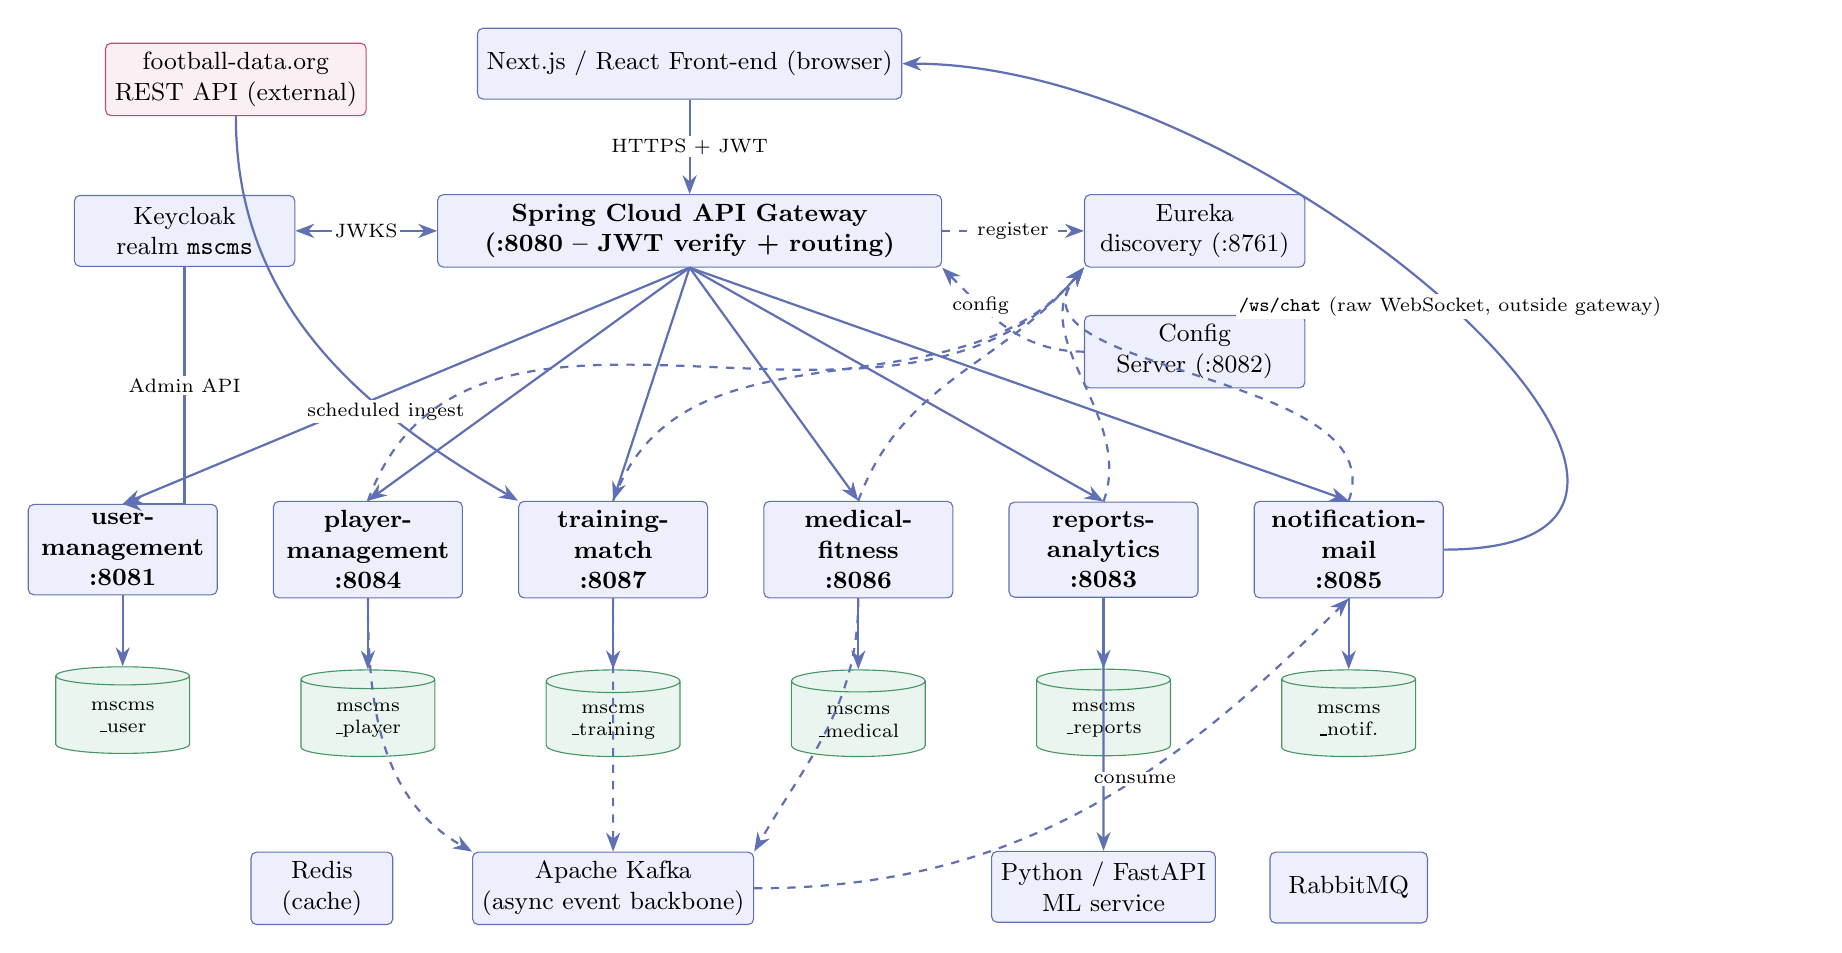
\begin{tikzpicture}[node distance=6mm and 7mm,
    every node/.style={transform shape}]

  % ---- frontend (browser) ----
  \node[comp, minimum width=50mm] (fe) {Next.js / React Front-end (browser)};

  % ---- API gateway ----
  \node[svc, below=12mm of fe, minimum width=64mm] (gw)
        {Spring Cloud API Gateway\\(:8080 -- JWT verify + routing)};

  % ---- identity provider (left of gateway) ----
  \node[comp, left=18mm of gw, minimum width=28mm] (kc)
        {Keycloak\\realm \texttt{mscms}};

  % ---- control plane (right of gateway) ----
  \node[comp, right=18mm of gw, minimum width=28mm] (eu) {Eureka\\discovery (:8761)};
  \node[comp, below=6mm of eu, minimum width=28mm] (cfg) {Config\\Server (:8082)};

  % ---- six domain services in a row ----
  \node[svc, below=30mm of gw, xshift=-72mm, minimum width=24mm] (um)
        {user-\\management\\:8081};
  \node[svc, right=of um, minimum width=24mm] (pm) {player-\\management\\:8084};
  \node[svc, right=of pm, minimum width=24mm] (tm) {training-\\match\\:8087};
  \node[svc, right=of tm, minimum width=24mm] (mf) {medical-\\fitness\\:8086};
  \node[svc, right=of mf, minimum width=24mm] (ra) {reports-\\analytics\\:8083};
  \node[svc, right=of ra, minimum width=24mm] (nm) {notification-\\mail\\:8085};

  % ---- per-service databases ----
  \node[store, below=9mm of um] (dbu) {mscms\\\_user};
  \node[store, below=9mm of pm] (dbp) {mscms\\\_player};
  \node[store, below=9mm of tm] (dbt) {mscms\\\_training};
  \node[store, below=9mm of mf] (dbm) {mscms\\\_medical};
  \node[store, below=9mm of ra] (dbr) {mscms\\\_reports};
  \node[store, below=9mm of nm] (dbn) {mscms\\\_notif.};

  % ---- external football API (far top-left corner) ----
  \node[ext, left=14mm of fe, yshift=-2mm, minimum width=32mm] (fd)
        {football-data.org\\REST API (external)};

  % ---- async / infra row (bottom) ----
  \node[comp, below=12mm of dbt, minimum width=32mm] (kafka)
        {Apache Kafka\\(async event backbone)};
  \node[comp, left=10mm of kafka, minimum width=18mm] (redis) {Redis\\(cache)};
  \node[comp, below=12mm of dbn, minimum width=20mm] (rmq) {RabbitMQ};
  \node[comp, below=12mm of dbr, minimum width=28mm] (ml)
        {Python / FastAPI\\ML service};

  % ===== synchronous edges =====
  \draw[flow] (fe) -- node[lbl,pos=0.5]{HTTPS + JWT} (gw);
  \draw[flow] (gw.south) -- (um.north);
  \draw[flow] (gw.south) -- (pm.north);
  \draw[flow] (gw.south) -- (tm.north);
  \draw[flow] (gw.south) -- (mf.north);
  \draw[flow] (gw.south) -- (ra.north);
  \draw[flow] (gw.south) -- (nm.north);

  % service -> own db
  \draw[flow] (um) -- (dbu);
  \draw[flow] (pm) -- (dbp);
  \draw[flow] (tm) -- (dbt);
  \draw[flow] (mf) -- (dbm);
  \draw[flow] (ra) -- (dbr);
  \draw[flow] (nm) -- (dbn);

  % keycloak JWT to gateway + Admin API to user-management
  \draw[biflow] (kc) -- node[lbl,pos=0.5]{JWKS} (gw);
  \draw[flow] (kc.south) -- node[lbl,pos=0.5]{Admin API} (um.north -| kc.south) -- (um.north);

  % training-match <- external API (scheduled ingestion)
  \draw[flow] (fd.south) to[out=-90,in=150]
        node[lbl,pos=0.7]{scheduled ingest} (tm.north west);

  % reports -> ML
  \draw[flow] (ra) -- (ml);

  % notification raw websocket to frontend (outside gateway)
  \draw[flow] (nm.east) to[out=0,in=0,looseness=1.3]
        node[lbl,pos=0.5]{\texttt{/ws/chat} (raw WebSocket, outside gateway)} (fe.east);

  % ===== control-plane (dashed: register / pull config) =====
  \draw[flowd] (gw.east) -- node[lbl,pos=0.5]{register} (eu.west);
  \draw[flowd] (cfg.west) to[out=180,in=-45] node[lbl,pos=0.7]{config} (gw.south east);
  \foreach \s in {pm,tm,mf,ra,nm}{ \draw[flowd] (\s.north) to[out=70,in=-130] (eu.south west); }

  % ===== async Kafka backbone =====
  \draw[flowd] (tm.south) to[out=-90,in=90] (kafka.north);
  \draw[flowd] (mf.south) to[out=-90,in=60] (kafka.north east);
  \draw[flowd] (pm.south) to[out=-90,in=150] (kafka.north west);
  \draw[flowd] (kafka.east) to[out=0,in=-135] node[lbl,pos=0.6]{consume} (nm.south);

\end{tikzpicture}%
}
\caption{High-level cloud-native microservices architecture of the platform: a Next.js front-end talks only to the Spring Cloud API Gateway, which routes authenticated traffic to six domain services, each owning a private PostgreSQL database, supported by a Eureka/Config control plane, Keycloak identity, a Kafka event backbone, Redis/RabbitMQ infrastructure, a Python/FastAPI ML service, and the external football-data.org feed.}
\label{fig-arch-overview}
\end{figure}


Figure~\ref{fig-arch-deploy} shows the same system from a deployment standpoint:
every component is a container orchestrated by Docker Compose on a single shared
network, grouped into infrastructure backing services, the Spring Cloud control
plane, the six domain services, the machine-learning service and the front-end.
This is the unit of reproducible deployment described in Appendix~\ref{app:deploy}.

\input{chapters/figs/arch-deploy}

%==============================================================================
\section{Use-Case Models}
\label{sec:design-usecase}

The platform serves many roles, each with a distinct surface of operations.
The following use-case diagrams group those operations by the actors that
perform them. Figure~\ref{fig-uc-admin} covers administration and club
management (the administrator, sport manager and team manager);
Figure~\ref{fig-uc-match} covers match and training operations (coaching staff
and analysts); Figure~\ref{fig-uc-medical} covers the medical and fitness staff;
and Figure~\ref{fig-uc-business} covers scouting, sponsorship and the read-only
surface presented to players and fans.

\input{chapters/figs/uc-admin}
% auto-generated figure: uc-match (source: wf)
\begin{figure}[H]
\centering
\resizebox{\textwidth}{!}{%
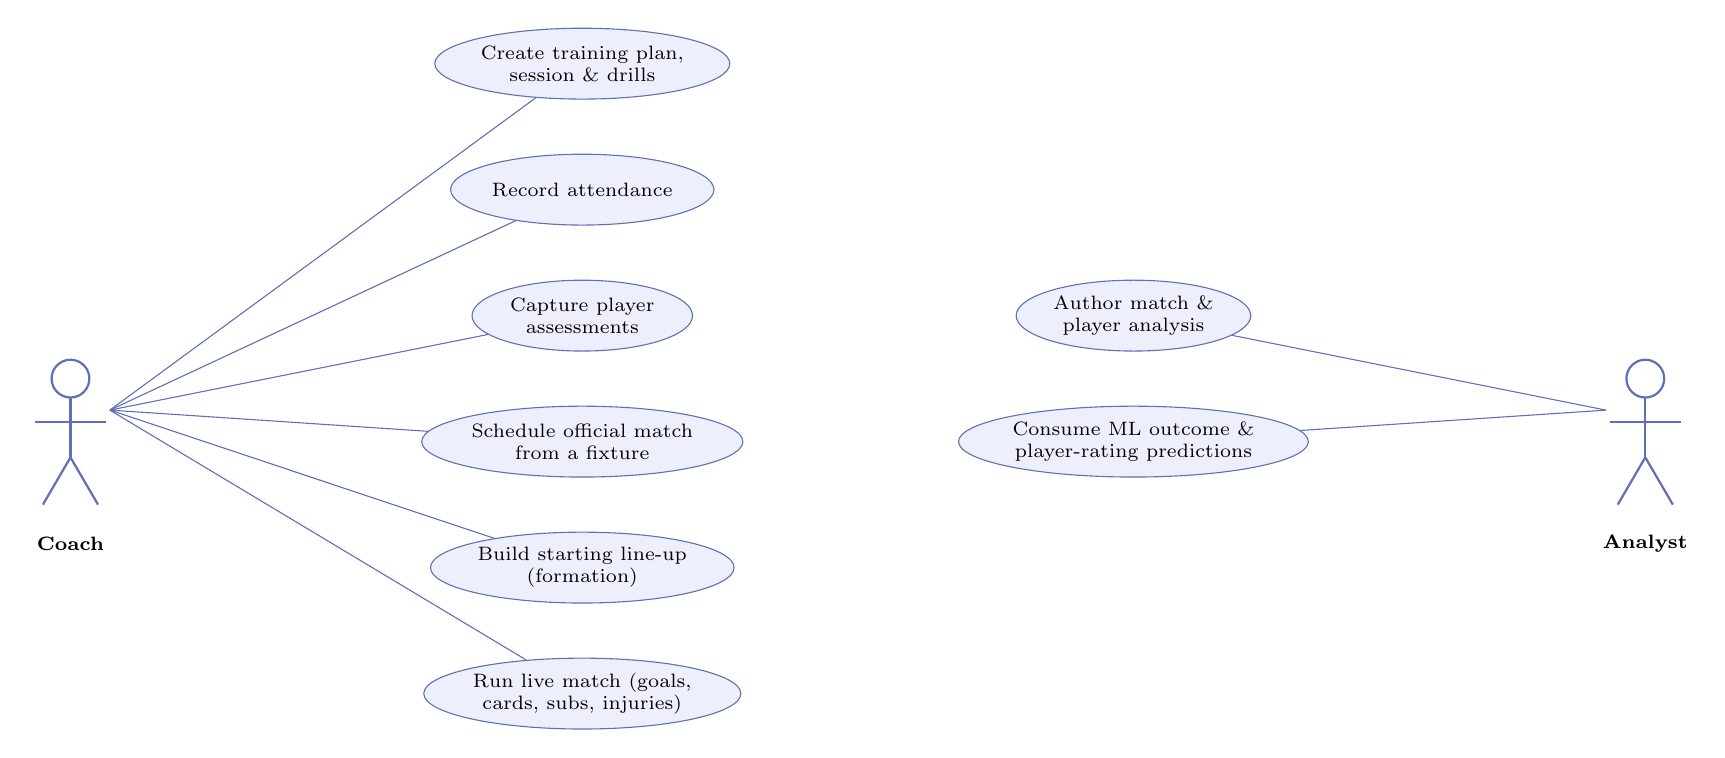
\begin{tikzpicture}
  % actors -- Coach on the left, Analyst on the right
  \UCactor{0}{0}{Coach}
  \UCactor{20}{0}{Analyst}

  % use cases -- training & match operations (Coach)
  \node[usecase] (u1) at (6.5,4.0){Create training plan,\\ session \& drills};
  \node[usecase] (u2) at (6.5,2.4){Record attendance};
  \node[usecase] (u3) at (6.5,0.8){Capture player\\ assessments};
  \node[usecase] (u4) at (6.5,-0.8){Schedule official match\\ from a fixture};
  \node[usecase] (u5) at (6.5,-2.4){Build starting line-up\\ (formation)};
  \node[usecase] (u6) at (6.5,-4.0){Run live match (goals,\\ cards, subs, injuries)};

  % use cases -- analysis & ML (Analyst)
  \node[usecase] (u7) at (13.5,0.8){Author match \&\\ player analysis};
  \node[usecase] (u8) at (13.5,-0.8){Consume ML outcome \&\\ player-rating predictions};

  % Coach associations
  \draw[dLine] (0.5,-0.4) -- (u1);
  \draw[dLine] (0.5,-0.4) -- (u2);
  \draw[dLine] (0.5,-0.4) -- (u3);
  \draw[dLine] (0.5,-0.4) -- (u4);
  \draw[dLine] (0.5,-0.4) -- (u5);
  \draw[dLine] (0.5,-0.4) -- (u6);

  % Analyst associations
  \draw[dLine] (19.5,-0.4) -- (u7);
  \draw[dLine] (19.5,-0.4) -- (u8);
\end{tikzpicture}%
}
\caption{Use-case diagram for match and training operations, in which the coach drives training planning and the line-up-mandatory match and live-match workflows while the analyst authors match and player analyses and consumes the machine-learning match-outcome and player-rating predictions.}
\label{fig-uc-match}
\end{figure}

% auto-generated figure: uc-medical (source: wf)
\begin{figure}[H]
\centering
\resizebox{\textwidth}{!}{%
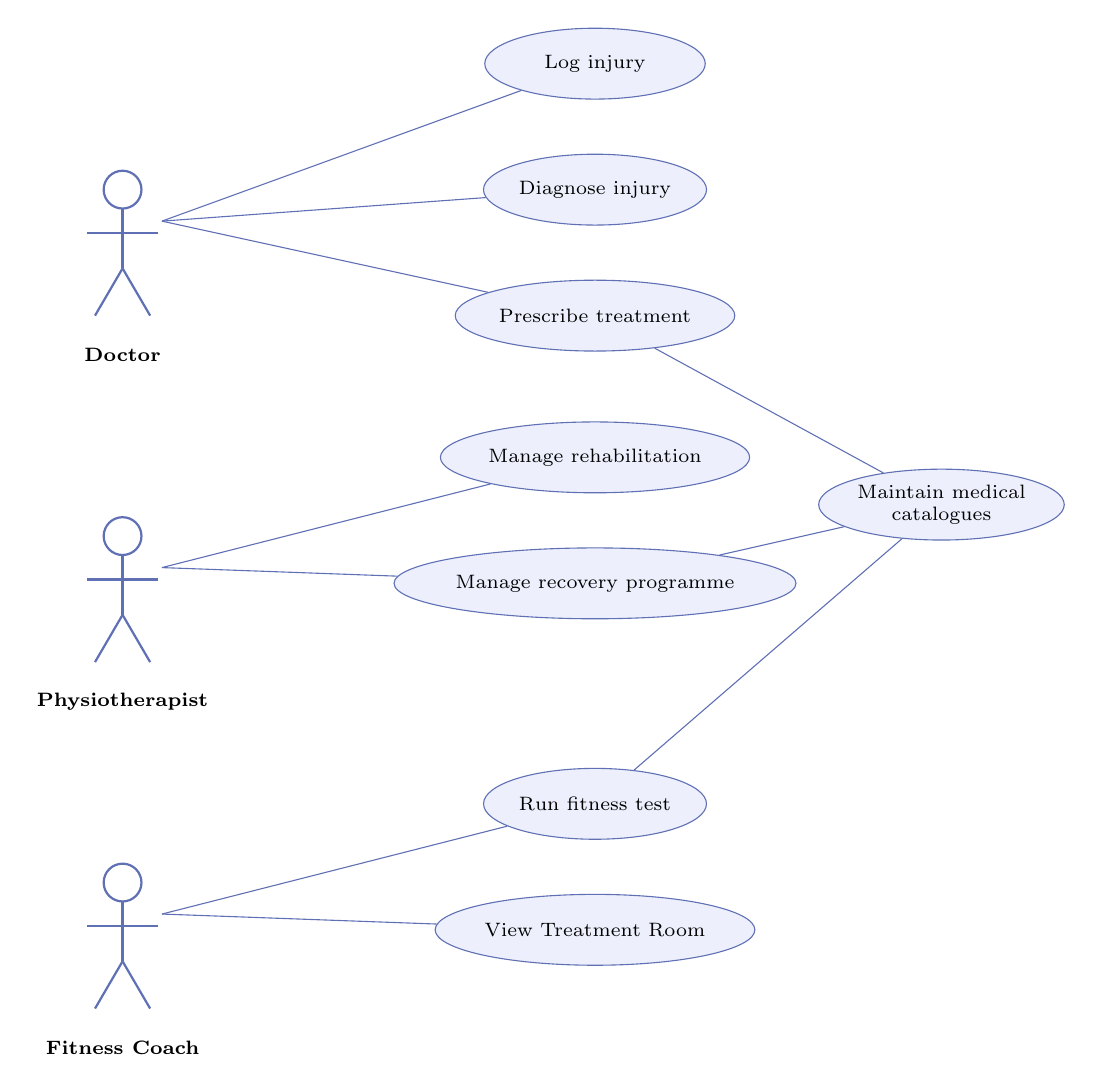
\begin{tikzpicture}
  % --- actors (left column) ---
  \UCactor{0}{4.4}{Doctor}
  \UCactor{0}{0}{Physiotherapist}
  \UCactor{0}{-4.4}{Fitness Coach}

  % --- use cases (right column) ---
  \node[usecase] (u1) at (6,6.0){Log injury};
  \node[usecase] (u2) at (6,4.4){Diagnose injury};
  \node[usecase] (u3) at (6,2.8){Prescribe treatment};
  \node[usecase] (u4) at (6,1.0){Manage rehabilitation};
  \node[usecase] (u5) at (6,-0.6){Manage recovery programme};
  \node[usecase] (u6) at (6,-3.4){Run fitness test};
  \node[usecase] (u7) at (6,-5.0){View Treatment Room};
  \node[usecase] (u8) at (10.4,0.4){Maintain medical\\ catalogues};

  % --- Doctor -> log / diagnose / treat ---
  \draw[dLine] (0.5,4.0) -- (u1);
  \draw[dLine] (0.5,4.0) -- (u2);
  \draw[dLine] (0.5,4.0) -- (u3);

  % --- Physiotherapist -> rehabilitation / recovery ---
  \draw[dLine] (0.5,-0.4) -- (u4);
  \draw[dLine] (0.5,-0.4) -- (u5);

  % --- Fitness Coach -> fitness test + treatment room ---
  \draw[dLine] (0.5,-4.8) -- (u6);
  \draw[dLine] (0.5,-4.8) -- (u7);

  % --- shared catalogue maintenance ---
  \draw[dLine] (u3) -- (u8);
  \draw[dLine] (u5) -- (u8);
  \draw[dLine] (u6) -- (u8);
\end{tikzpicture}%
}
\caption{Use-case diagram for the medical and fitness module, mapping the Doctor, Physiotherapist and Fitness Coach to the staged injury-to-recovery workflow and the shared medical catalogues.}
\label{fig-uc-medical}
\end{figure}

\input{chapters/figs/uc-business}

%==============================================================================
\section{Class and Domain Models}
\label{sec:design-class}

The relational schema is materialised in the running services as a set of JPA
entity classes related by composition (an owning parent that manages the life
cycle of its children) and by reference (an identifier the application resolves
on demand). The class diagrams below capture each subsystem in turn. The user
identity model (Figure~\ref{fig-class-user}) shows the central \texttt{User}
specialised by a one-to-one profile per role. The squad model
(Figure~\ref{fig-class-squad}) expresses the team hierarchy and the transfer
market. The match and training model (Figure~\ref{fig-class-match}) and the
competition model (Figure~\ref{fig-class-competition}) show why a match, its
formation and its starting line-up form a single atomic aggregate. The medical
model (Figure~\ref{fig-class-medical}) encodes the recovery journey as a
composition hierarchy rooted at \texttt{Injury}, and the communication
(Figure~\ref{fig-class-comm}) and analytics (Figure~\ref{fig-class-reports})
models complete the picture.

% auto-generated figure: class-user (source: wf)
\begin{figure}[H]
\centering
\resizebox{\textwidth}{!}{%
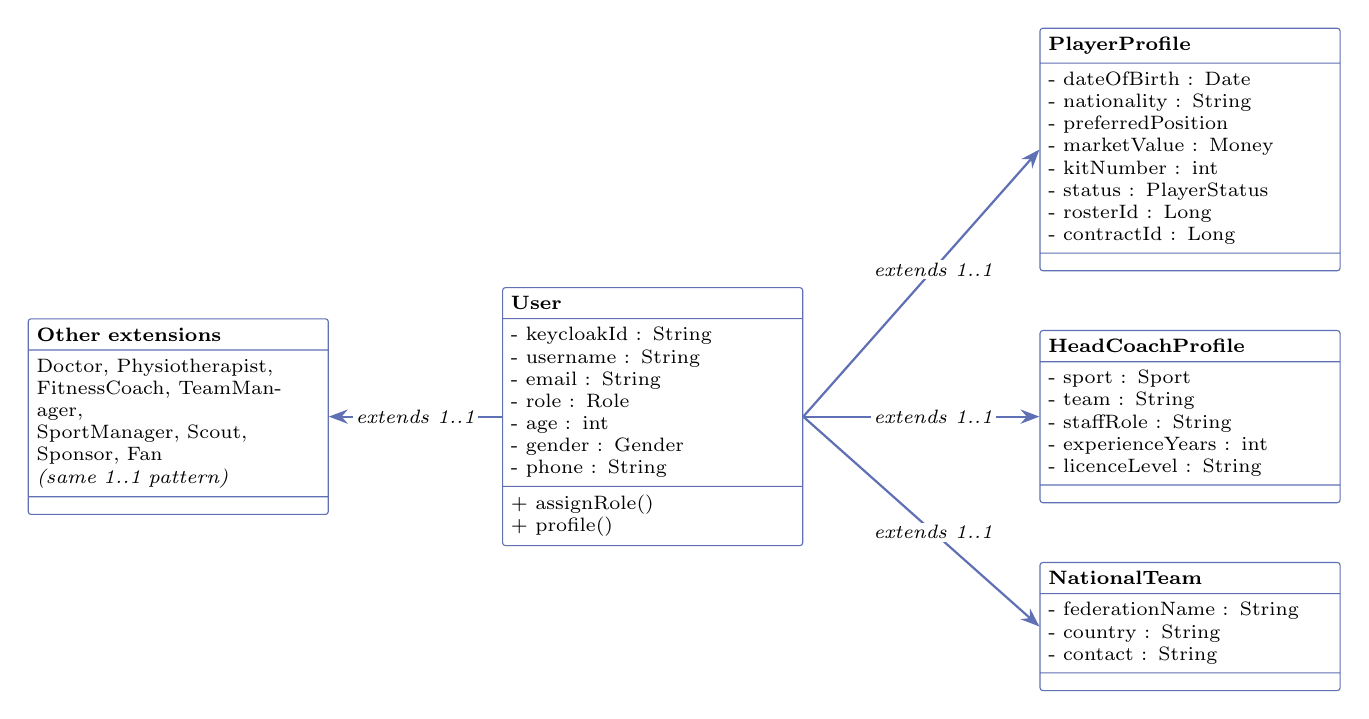
\begin{tikzpicture}[node distance=10mm]
  % --- central identity class ---
  \UmlClass{user}{User}{%
    - keycloakId : String\\
    - username : String\\
    - email : String\\
    - role : Role\\
    - age : int\\
    - gender : Gender\\
    - phone : String}{%
    + assignRole()\\
    + profile()}

  % --- role-extension classes (vertical extension, 1..1) ---
  \UmlClass[above right=2mm and 30mm of user]{player}{PlayerProfile}{%
    - dateOfBirth : Date\\
    - nationality : String\\
    - preferredPosition\\
    - marketValue : Money\\
    - kitNumber : int\\
    - status : PlayerStatus\\
    - rosterId : Long\\
    - contractId : Long}{}

  \UmlClass[right=30mm of user]{coach}{HeadCoachProfile}{%
    - sport : Sport\\
    - team : String\\
    - staffRole : String\\
    - experienceYears : int\\
    - licenceLevel : String}{}

  \UmlClass[below right=2mm and 30mm of user]{nteam}{NationalTeam}{%
    - federationName : String\\
    - country : String\\
    - contact : String}{}

  % --- note: further role extensions ---
  \UmlClass[left=22mm of user]{others}{Other extensions}{%
    Doctor, Physiotherapist,\\
    FitnessCoach, TeamManager,\\
    SportManager, Scout,\\
    Sponsor, Fan\\
    \emph{(same 1..1 pattern)}}{}

  % --- composition links: User extends each profile 1..1 ---
  \draw[flow] (user.east) -- node[lbl,pos=0.55]{\itshape extends 1..1} (player.west);
  \draw[flow] (user.east) -- node[lbl,pos=0.55]{\itshape extends 1..1} (coach.west);
  \draw[flow] (user.east) -- node[lbl,pos=0.55]{\itshape extends 1..1} (nteam.west);
  \draw[flow] (user.west) -- node[lbl,pos=0.5]{\itshape extends 1..1} (others.east);
\end{tikzpicture}}
\caption{Class model of the user-management domain: the central \texttt{User} identity record and its one-to-one role-extension classes (\texttt{PlayerProfile}, \texttt{HeadCoachProfile}, \texttt{NationalTeam} and the remaining role extensions), realising the vertical-extension pattern of \texttt{mscms\_user}.}
\label{fig-class-user}
\end{figure}

\input{chapters/figs/class-squad}
\input{chapters/figs/class-match}
% auto-generated figure: class-competition (source: wf)
\begin{figure}[H]
\centering
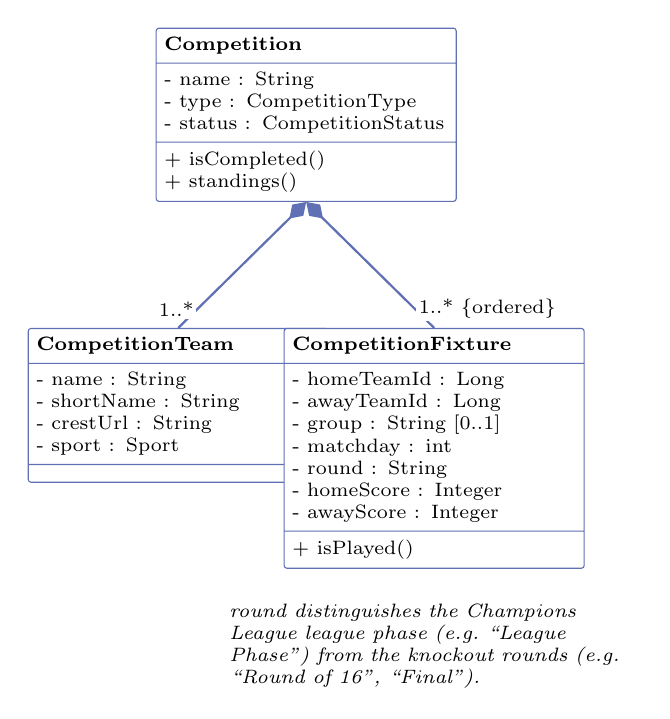
\begin{tikzpicture}[node distance=10mm]
  \UmlClass{comp}{Competition}{%
    - name : String\\
    - type : CompetitionType\\
    - status : CompetitionStatus}{%
    + isCompleted()\\
    + standings()}
  \UmlClass[below left=16mm and -22mm of comp]{team}{CompetitionTeam}{%
    - name : String\\
    - shortName : String\\
    - crestUrl : String\\
    - sport : Sport}{}
  \UmlClass[below right=16mm and -22mm of comp]{fix}{CompetitionFixture}{%
    - homeTeamId : Long\\
    - awayTeamId : Long\\
    - group : String [0..1]\\
    - matchday : int\\
    - round : String\\
    - homeScore : Integer\\
    - awayScore : Integer}{%
    + isPlayed()}

  % compositions (filled diamond at the Competition / whole end)
  \draw[{Diamond[fill=dLine,length=3mm,width=2mm]}-,draw=dLine,thick]
        (comp.south) -- node[lbl,pos=0.85,left]{1..*} (team.north);
  \draw[{Diamond[fill=dLine,length=3mm,width=2mm]}-,draw=dLine,thick]
        (comp.south) -- node[lbl,pos=0.85,right]{1..* \{ordered\}} (fix.north);

  \node[lbl,align=left,text width=52mm,font=\scriptsize,
        below=4mm of fix.south,anchor=north]
       {\itshape round distinguishes the Champions League league
        phase (e.g.\ ``League Phase'') from the knockout rounds
        (e.g.\ ``Round of 16'', ``Final'').};
\end{tikzpicture}
\caption{Class model of the competitions domain: a Competition composes its participating CompetitionTeam rows and its ordered CompetitionFixture rows, whose round label separates the Champions League league phase from the knockout rounds.}
\label{fig-class-competition}
\end{figure}

\input{chapters/figs/class-medical}
% auto-generated figure: class-comm (source: wf)
\begin{figure}[H]
\centering
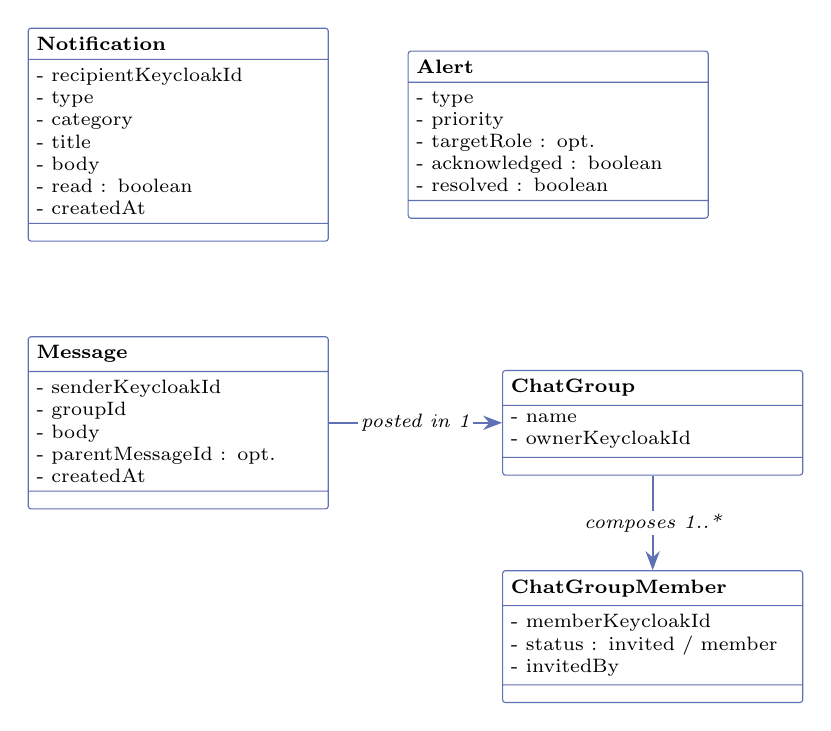
\begin{tikzpicture}[node distance=10mm]
  \UmlClass{notif}{Notification}{%
    - recipientKeycloakId\\
    - type\\
    - category\\
    - title\\
    - body\\
    - read : boolean\\
    - createdAt}{}
  \UmlClass[right=10mm of notif]{alert}{Alert}{%
    - type\\
    - priority\\
    - targetRole : opt.\\
    - acknowledged : boolean\\
    - resolved : boolean}{}
  \UmlClass[below=12mm of notif]{msg}{Message}{%
    - senderKeycloakId\\
    - groupId\\
    - body\\
    - parentMessageId : opt.\\
    - createdAt}{}
  \UmlClass[right=22mm of msg]{grp}{ChatGroup}{%
    - name\\
    - ownerKeycloakId}{}
  \UmlClass[below=12mm of grp]{mem}{ChatGroupMember}{%
    - memberKeycloakId\\
    - status : invited / member\\
    - invitedBy}{}

  % composition: ChatGroup composes 1..* ChatGroupMember
  \draw[flow] (grp) -- node[lbl,pos=0.5]{\itshape composes 1..*} (mem);
  % reference: Message -> ChatGroup
  \draw[flow] (msg) -- node[lbl,pos=0.5]{\itshape posted in 1} (grp.west);
\end{tikzpicture}
\caption{Class model of the communication subsystem (\texttt{mscms\_notification}), showing per-recipient notifications, role-targeted alerts, threaded messages, and chat groups that compose their members.}
\label{fig-class-comm}
\end{figure}

% auto-generated figure: class-reports (source: wf)
\begin{figure}[H]
\centering
\resizebox{\textwidth}{!}{%
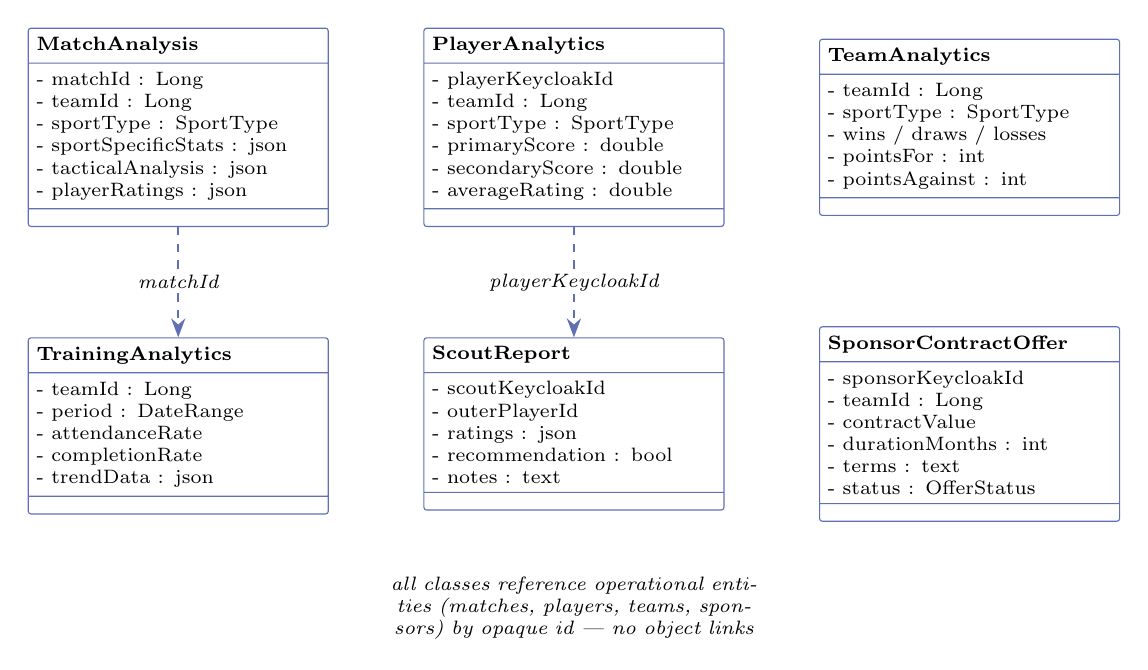
\begin{tikzpicture}[node distance=10mm]
  \UmlClass{ma}{MatchAnalysis}{%
    - matchId : Long\\
    - teamId : Long\\
    - sportType : SportType\\
    - sportSpecificStats : json\\
    - tacticalAnalysis : json\\
    - playerRatings : json}{}
  \UmlClass[right=12mm of ma]{pa}{PlayerAnalytics}{%
    - playerKeycloakId\\
    - teamId : Long\\
    - sportType : SportType\\
    - primaryScore : double\\
    - secondaryScore : double\\
    - averageRating : double}{}
  \UmlClass[right=12mm of pa]{ta}{TeamAnalytics}{%
    - teamId : Long\\
    - sportType : SportType\\
    - wins / draws / losses\\
    - pointsFor : int\\
    - pointsAgainst : int}{}
  \UmlClass[below=14mm of ma]{tr}{TrainingAnalytics}{%
    - teamId : Long\\
    - period : DateRange\\
    - attendanceRate\\
    - completionRate\\
    - trendData : json}{}
  \UmlClass[below=14mm of pa]{sr}{ScoutReport}{%
    - scoutKeycloakId\\
    - outerPlayerId\\
    - ratings : json\\
    - recommendation : bool\\
    - notes : text}{}
  \UmlClass[below=14mm of ta]{so}{SponsorContractOffer}{%
    - sponsorKeycloakId\\
    - teamId : Long\\
    - contractValue\\
    - durationMonths : int\\
    - terms : text\\
    - status : OfferStatus}{}

  % relationship notes: opaque-id references, no object links
  \draw[flowd] (ma) -- node[lbl,pos=0.5]{\itshape matchId} (tr);
  \draw[flowd] (pa) -- node[lbl,pos=0.5]{\itshape playerKeycloakId} (sr);
  \node[lbl,below=8mm of sr,text width=70mm,align=center]
        {\itshape all classes reference operational entities
         (matches, players, teams, sponsors) by opaque id --- no object links};
\end{tikzpicture}}
\caption{Class model of the reports-and-analytics domain (\texttt{mscms\_reports}): six authored or derived classes that aggregate operational data over a period and reference matches, players, teams and sponsors only by opaque identifier rather than by object links.}
\label{fig-class-reports}
\end{figure}


%==============================================================================
\section{Entity-Relationship (Database) Models}
\label{sec:design-er}

Because every domain service owns its own database, the data model is best
presented one database at a time. Each diagram shows the principal tables of a
service database, their primary and foreign keys and the relationships between
them. Figure~\ref{fig-er-user} models the user database with its central
\texttt{user} table and per-role extension tables;
Figure~\ref{fig-er-player} the squad and transfer market;
Figure~\ref{fig-er-training} the (largest) training, match and competition
schema; Figure~\ref{fig-er-medical} the injury aggregate and independent
measurement tables; Figure~\ref{fig-er-notification} the notification,
alerting and group-chat tables; and Figure~\ref{fig-er-reports} the derived
analytics and authored artefacts, which reference the operational domains only
by opaque identifier.

% auto-generated figure: er-user (source: wf)
\begin{figure}[H]
\centering
\resizebox{\textwidth}{!}{%
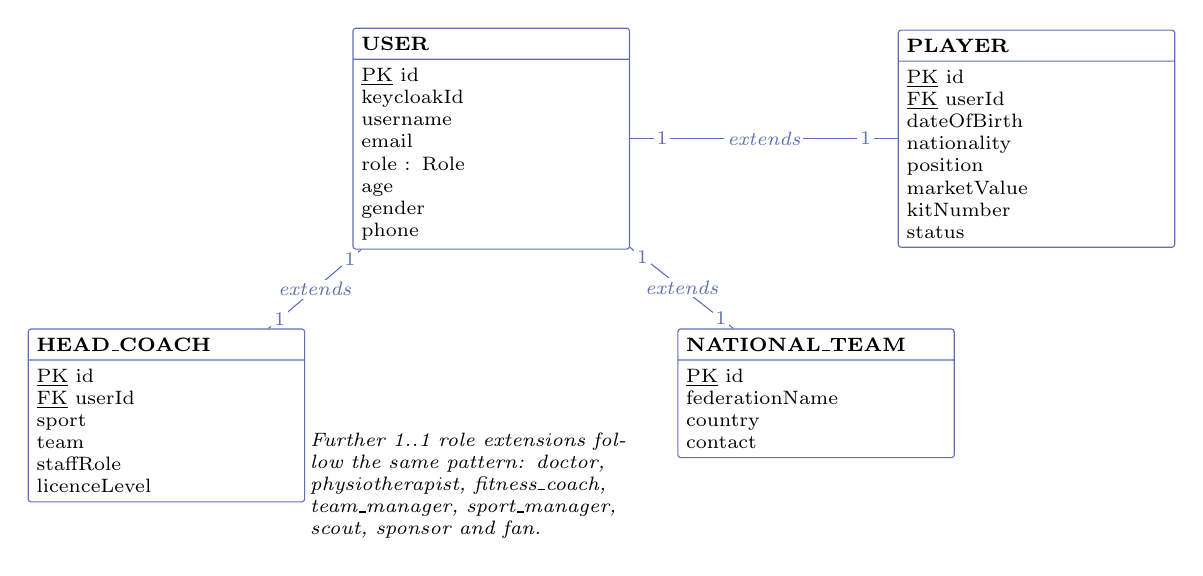
\begin{tikzpicture}[node distance=14mm]
  \Entity{usr}{USER}{%
    \underline{PK} id\\ keycloakId\\ username\\ email\\ role : Role\\ age\\ gender\\ phone}
  \Entity[right=34mm of usr]{ply}{PLAYER}{%
    \underline{PK} id\\ \underline{FK} userId\\ dateOfBirth\\ nationality\\ position\\ marketValue\\ kitNumber\\ status}
  \Entity[below left=10mm and 6mm of usr]{coa}{HEAD\_COACH}{%
    \underline{PK} id\\ \underline{FK} userId\\ sport\\ team\\ staffRole\\ licenceLevel}
  \Entity[below right=10mm and 6mm of usr]{nat}{NATIONAL\_TEAM}{%
    \underline{PK} id\\ federationName\\ country\\ contact}
  \Rel{usr}{ply}{1}{1}{extends}
  \Rel{usr}{coa}{1}{1}{extends}
  \Rel{usr}{nat}{1}{1}{extends}
  \node[font=\scriptsize\itshape, text width=46mm, align=left,
        below=22mm of usr] (note)
    {Further 1..1 role extensions follow the same pattern: doctor, physiotherapist,
     fitness\_coach, team\_manager, sport\_manager, scout, sponsor and fan.};
\end{tikzpicture}%
}
\caption{Entity-relationship diagram of the \texttt{mscms\_user} database, showing the common USER identity record and its one-to-one per-role profile extensions (PLAYER, HEAD\_COACH, NATIONAL\_TEAM, and the remaining role tables).}
\label{fig-er-user}
\end{figure}

\input{chapters/figs/er-player}
% auto-generated figure: er-training (source: wf)
\begin{figure}[H]
\centering
\resizebox{\textwidth}{!}{%
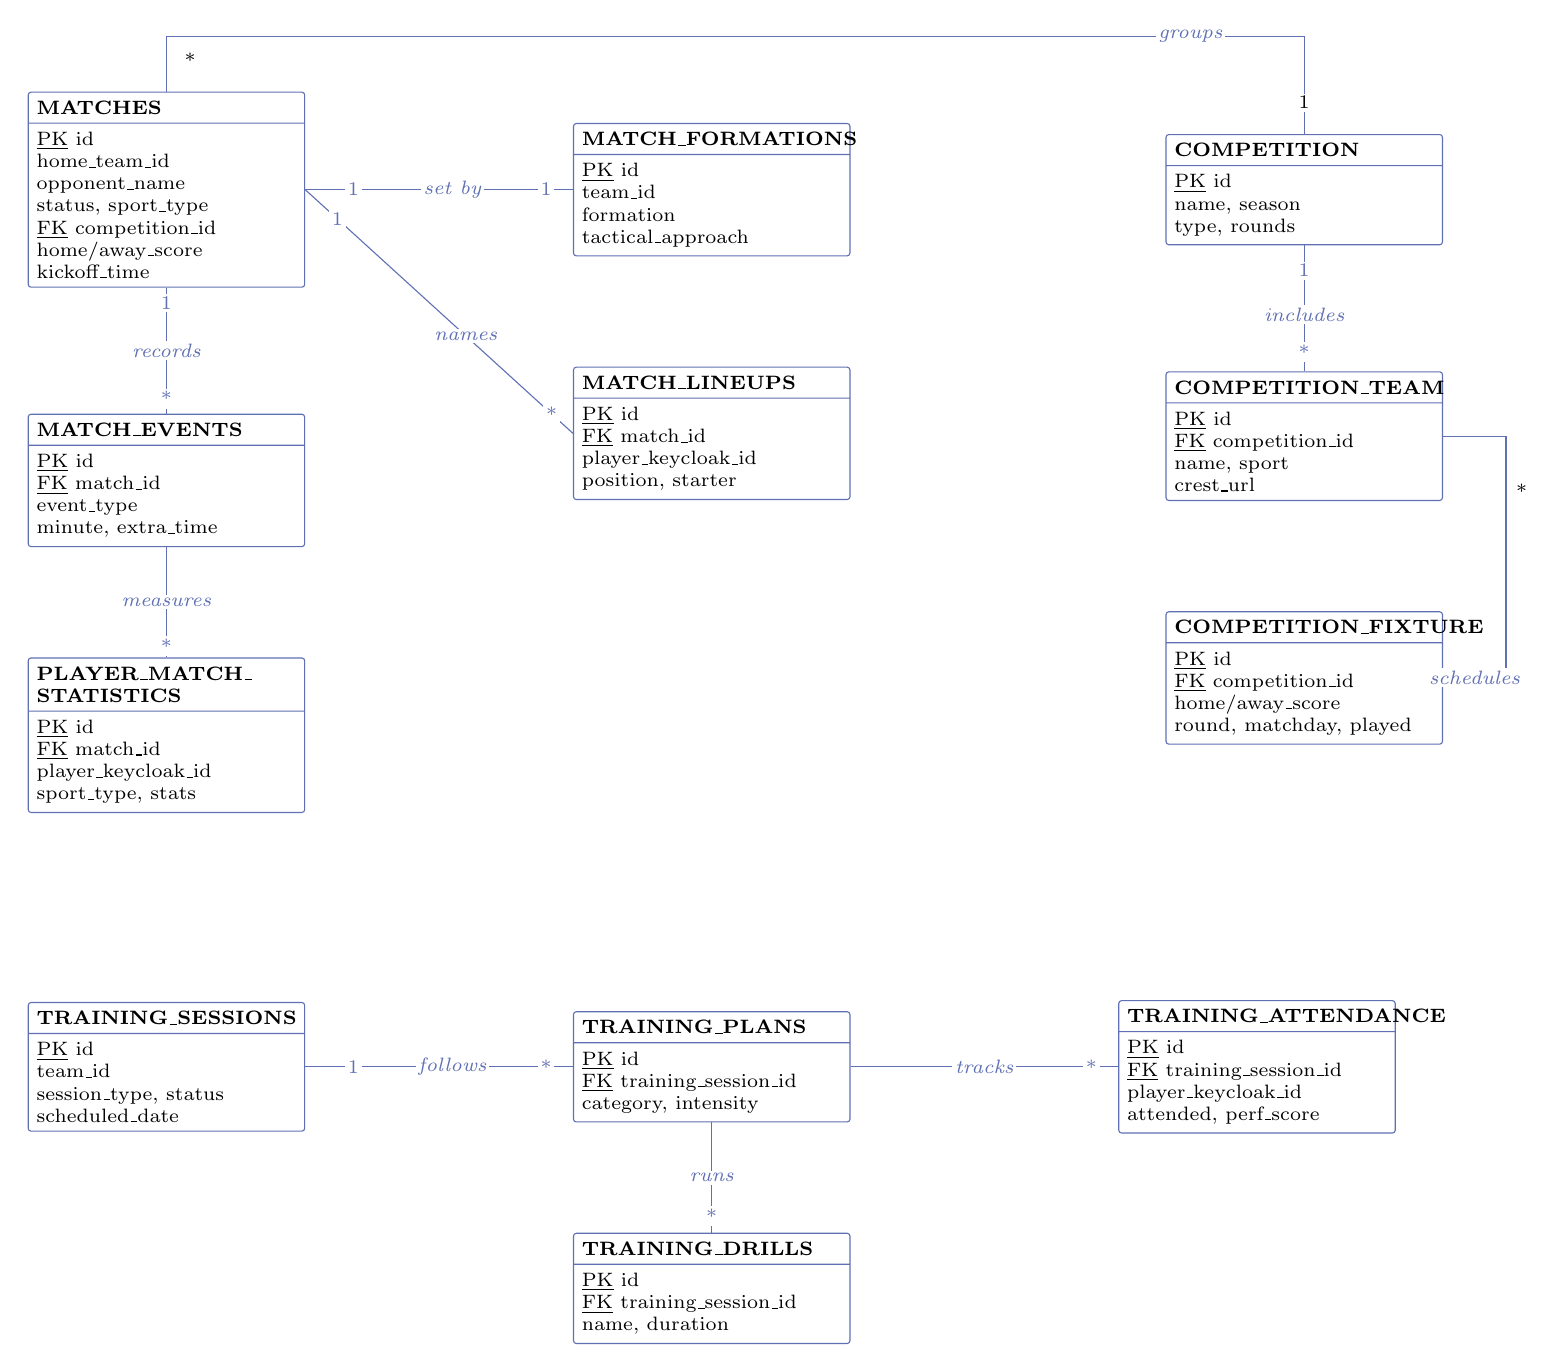
\begin{tikzpicture}[node distance=10mm,
    every node/.append style={font=\scriptsize}]

  % ===== Matches cluster (left/centre) ==================================
  \Entity{m}{MATCHES}{%
    \underline{PK} id\\
    home\_team\_id\\
    opponent\_name\\
    status, sport\_type\\
    \underline{FK} competition\_id\\
    home/away\_score\\
    kickoff\_time}
  % formations / lineups stacked to the right of MATCHES
  \Entity[right=34mm of m]{mf}{MATCH\_FORMATIONS}{%
    \underline{PK} id\\
    team\_id\\
    formation\\
    tactical\_approach}
  \Entity[below=14mm of mf]{ml}{MATCH\_LINEUPS}{%
    \underline{PK} id\\
    \underline{FK} match\_id\\
    player\_keycloak\_id\\
    position, starter}
  % events / statistics stacked below MATCHES
  \Entity[below=16mm of m]{me}{MATCH\_EVENTS}{%
    \underline{PK} id\\
    \underline{FK} match\_id\\
    event\_type\\
    minute, extra\_time}
  \Entity[below=14mm of me]{pms}{PLAYER\_MATCH\_\\STATISTICS}{%
    \underline{PK} id\\
    \underline{FK} match\_id\\
    player\_keycloak\_id\\
    sport\_type, stats}

  % ===== Competition cluster (right) ====================================
  \Entity[right=40mm of mf]{cmp}{COMPETITION}{%
    \underline{PK} id\\
    name, season\\
    type, rounds}
  \Entity[below=16mm of cmp]{ct}{COMPETITION\_TEAM}{%
    \underline{PK} id\\
    \underline{FK} competition\_id\\
    name, sport\\
    crest\_url}
  \Entity[below=14mm of ct]{cf}{COMPETITION\_FIXTURE}{%
    \underline{PK} id\\
    \underline{FK} competition\_id\\
    home/away\_score\\
    round, matchday, played}

  % ===== Training cluster (bottom row) ==================================
  \Entity[below=24mm of pms]{ts}{TRAINING\_SESSIONS}{%
    \underline{PK} id\\
    team\_id\\
    session\_type, status\\
    scheduled\_date}
  \Entity[right=34mm of ts]{tp}{TRAINING\_PLANS}{%
    \underline{PK} id\\
    \underline{FK} training\_session\_id\\
    category, intensity}
  \Entity[below=14mm of tp]{td}{TRAINING\_DRILLS}{%
    \underline{PK} id\\
    \underline{FK} training\_session\_id\\
    name, duration}
  \Entity[right=34mm of tp]{ta}{TRAINING\_ATTENDANCE}{%
    \underline{PK} id\\
    \underline{FK} training\_session\_id\\
    player\_keycloak\_id\\
    attended, perf\_score}

  % ===== Relationships : MATCHES hub ===================================
  % to formations (right) and lineups (lower-right) from the right edge
  \draw[dLine] (m.east) -- node[lbl,pos=0.18]{1} node[lbl,pos=0.55]{\itshape set by}
       node[lbl,pos=0.9]{1} (mf.west);
  \draw[dLine] (m.east) -- node[lbl,pos=0.12]{1} node[lbl,pos=0.6]{\itshape names}
       node[lbl,pos=0.92]{*} (ml.west);
  % to events / statistics straight down
  \Rel{m}{me}{1}{*}{records}
  \draw[dLine] (me.south) -- node[lbl,pos=0.5]{\itshape measures}
       node[lbl,pos=0.9]{*} (pms.north);

  % ===== Relationships : COMPETITION hub ===============================
  % COMPETITION 1--* MATCHES (competition_id FK) routed over the top so it
  % never crosses the formations/lineups boxes
  \draw[dLine] (cmp.north) |- ($(m.north)+(0,7mm)$)
       node[lbl,pos=0.55]{\itshape groups} -- (m.north);
  \node[lbl] at ($(cmp.north)+(0,4mm)$){1};
  \node[lbl] at ($(m.north)+(3mm,4mm)$){*};
  % vertical chain, offset so it never crosses a box
  \draw[dLine] (cmp.south) -- node[lbl,pos=0.2]{1} node[lbl,pos=0.55]{\itshape includes}
       node[lbl,pos=0.85]{*} (ct.north);
  \draw[dLine] (ct.east) -- ++(8mm,0) |- node[lbl,pos=0.75]{\itshape schedules} (cf.east);
  \node[lbl] at ($(ct.east)+(10mm,-7mm)$){*};

  % ===== Relationships : TRAINING hub ==================================
  \draw[dLine] (ts.east) -- node[lbl,pos=0.18]{1} node[lbl,pos=0.55]{\itshape follows}
       node[lbl,pos=0.9]{*} (tp.west);
  \draw[dLine] (tp.south) -- node[lbl,pos=0.5]{\itshape runs}
       node[lbl,pos=0.85]{*} (td.north);
  \draw[dLine] (tp.east) -- node[lbl,pos=0.5]{\itshape tracks}
       node[lbl,pos=0.9]{*} (ta.west);

\end{tikzpicture}%
}
\caption{Entity-relationship diagram of the \texttt{mscms\_training} database, showing the matches subsystem (formations, line-ups, events and per-player statistics), the database-backed competition subsystem (teams and fixtures), and the training subsystem (plans, drills and attendance) with their principal columns and foreign-key relationships.}
\label{fig-er-training}
\end{figure}

% auto-generated figure: er-medical (source: wf)
\begin{figure}[H]
\centering
\resizebox{\textwidth}{!}{%
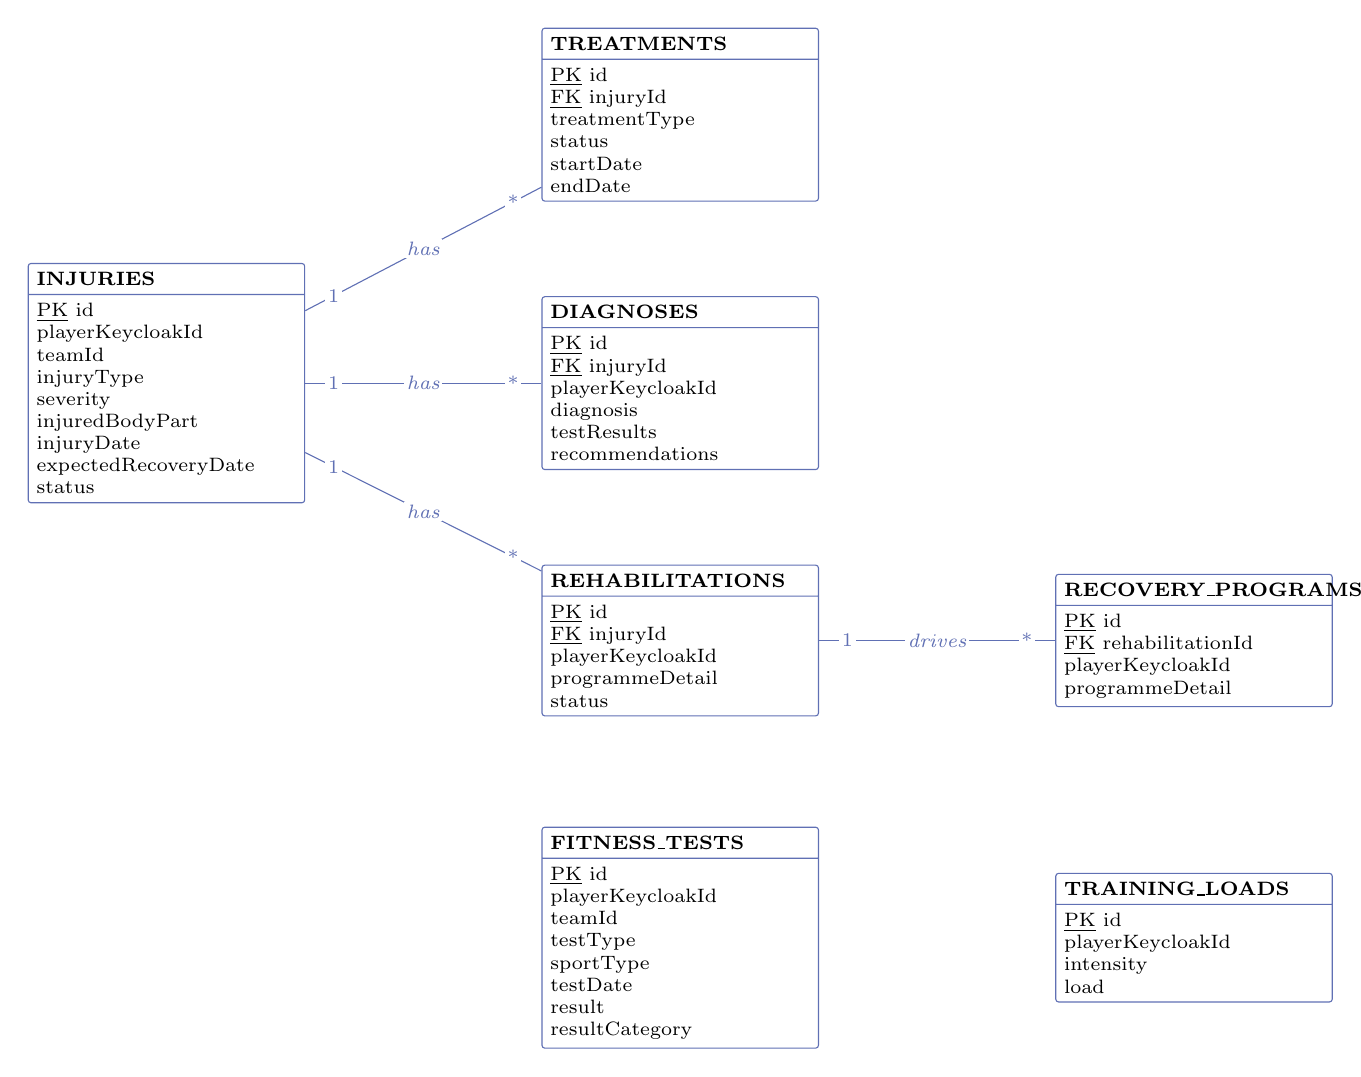
\begin{tikzpicture}[node distance=14mm]
  % central injury record and its staged journey
  \Entity{inj}{INJURIES}{%
    \underline{PK} id\\
    playerKeycloakId\\
    teamId\\
    injuryType\\
    severity\\
    injuredBodyPart\\
    injuryDate\\
    expectedRecoveryDate\\
    status}
  \Entity[right=30mm of inj]{dia}{DIAGNOSES}{%
    \underline{PK} id\\
    \underline{FK} injuryId\\
    playerKeycloakId\\
    diagnosis\\
    testResults\\
    recommendations}
  \Entity[above=12mm of dia]{trt}{TREATMENTS}{%
    \underline{PK} id\\
    \underline{FK} injuryId\\
    treatmentType\\
    status\\
    startDate\\
    endDate}
  \Entity[below=12mm of dia]{reh}{REHABILITATIONS}{%
    \underline{PK} id\\
    \underline{FK} injuryId\\
    playerKeycloakId\\
    programmeDetail\\
    status}
  \Entity[right=30mm of reh]{rec}{RECOVERY\_PROGRAMS}{%
    \underline{PK} id\\
    \underline{FK} rehabilitationId\\
    playerKeycloakId\\
    programmeDetail}
  % independent fitness / load entities
  \Entity[below=14mm of reh]{fit}{FITNESS\_TESTS}{%
    \underline{PK} id\\
    playerKeycloakId\\
    teamId\\
    testType\\
    sportType\\
    testDate\\
    result\\
    resultCategory}
  \Entity[right=30mm of fit]{tld}{TRAINING\_LOADS}{%
    \underline{PK} id\\
    playerKeycloakId\\
    intensity\\
    load}
  % relationships
  \Rel{inj}{trt}{1}{*}{has}
  \Rel{inj}{dia}{1}{*}{has}
  \Rel{inj}{reh}{1}{*}{has}
  \Rel{reh}{rec}{1}{*}{drives}
\end{tikzpicture}%
}
\caption{Entity-relationship diagram for the \texttt{mscms\_medical} database, showing the staged injury journey (injuries owning diagnoses, treatments and rehabilitations, with rehabilitations driving recovery programmes) alongside the independent fitness-test and training-load records.}
\label{fig-er-medical}
\end{figure}

% auto-generated figure: er-notification (source: wf)
\begin{figure}[H]
\centering
\resizebox{\textwidth}{!}{%
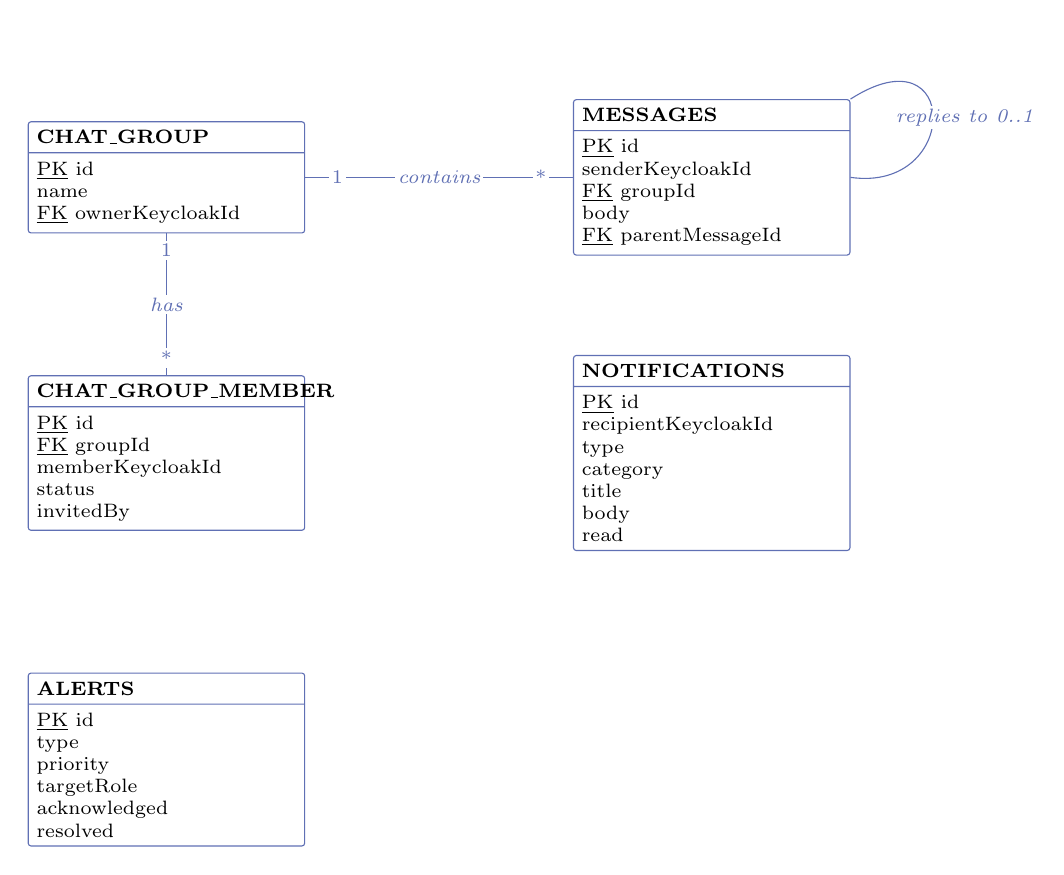
\begin{tikzpicture}[node distance=16mm]
  \Entity{cg}{CHAT\_GROUP}{%
    \underline{PK} id\\ name\\ \underline{FK} ownerKeycloakId}
  \Entity[below=18mm of cg]{cgm}{CHAT\_GROUP\_MEMBER}{%
    \underline{PK} id\\ \underline{FK} groupId\\ memberKeycloakId\\ status\\ invitedBy}
  \Entity[right=34mm of cg]{msg}{MESSAGES}{%
    \underline{PK} id\\ senderKeycloakId\\ \underline{FK} groupId\\ body\\ \underline{FK} parentMessageId}
  \Entity[right=34mm of cgm]{ntf}{NOTIFICATIONS}{%
    \underline{PK} id\\ recipientKeycloakId\\ type\\ category\\ title\\ body\\ read}
  \Entity[below=18mm of cgm]{alr}{ALERTS}{%
    \underline{PK} id\\ type\\ priority\\ targetRole\\ acknowledged\\ resolved}
  \Rel{cg}{cgm}{1}{*}{has}
  \Rel{cg}{msg}{1}{*}{contains}
  \draw[dLine] (msg.north east) .. controls +(1.4,0.9) and +(1.4,-0.2) ..
       node[lbl,pos=0.5,xshift=4mm]{\itshape replies to 0..1} (msg.east);
\end{tikzpicture}%
}
\caption{Entity-relationship diagram of the \texttt{mscms\_notification} database, showing notifications, alerts, and the team-chat groups, members, and threaded messages.}
\label{fig-er-notification}
\end{figure}

% auto-generated figure: er-reports (source: wf)
\begin{figure}[H]
\centering
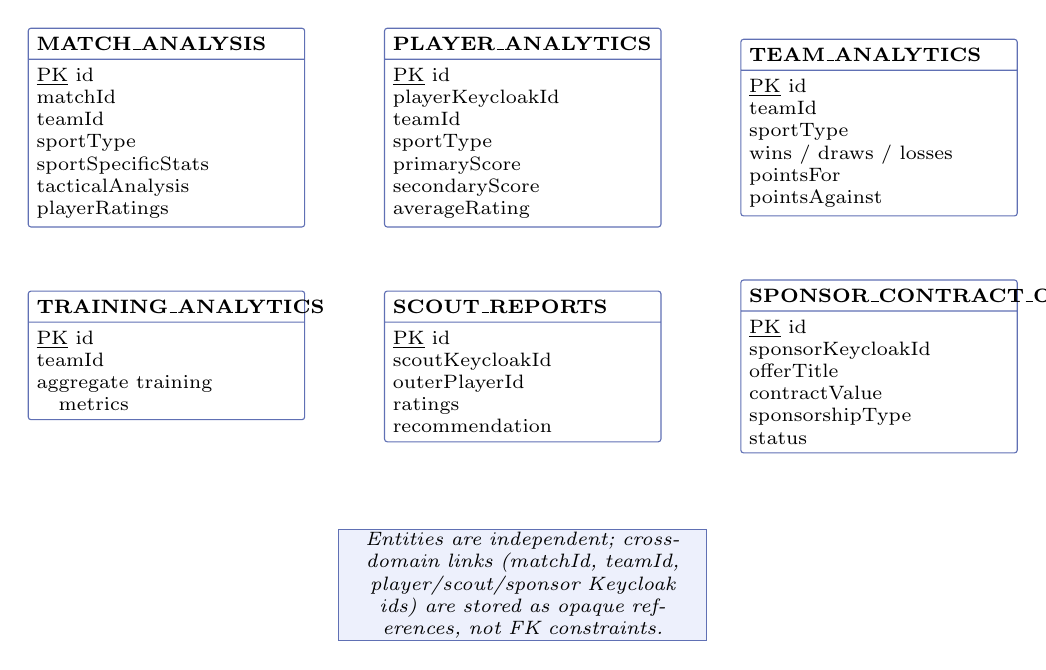
\begin{tikzpicture}[node distance=8mm]
  \Entity{ma}{MATCH\_ANALYSIS}{%
    \underline{PK} id\\
    matchId\\
    teamId\\
    sportType\\
    sportSpecificStats\\
    tacticalAnalysis\\
    playerRatings}
  \Entity[right=10mm of ma]{pa}{PLAYER\_ANALYTICS}{%
    \underline{PK} id\\
    playerKeycloakId\\
    teamId\\
    sportType\\
    primaryScore\\
    secondaryScore\\
    averageRating}
  \Entity[right=10mm of pa]{ta}{TEAM\_ANALYTICS}{%
    \underline{PK} id\\
    teamId\\
    sportType\\
    wins / draws / losses\\
    pointsFor\\
    pointsAgainst}
  \Entity[below=8mm of ma]{tr}{TRAINING\_ANALYTICS}{%
    \underline{PK} id\\
    teamId\\
    aggregate training\\ \quad metrics}
  \Entity[below=8mm of pa]{sr}{SCOUT\_REPORTS}{%
    \underline{PK} id\\
    scoutKeycloakId\\
    outerPlayerId\\
    ratings\\
    recommendation}
  \Entity[below=8mm of ta]{sc}{SPONSOR\_CONTRACT\_OFFERS}{%
    \underline{PK} id\\
    sponsorKeycloakId\\
    offerTitle\\
    contractValue\\
    sponsorshipType\\
    status}
  \node[lbl, draw=dLine, fill=dFill, text width=46mm, align=center,
        below=11mm of sr] (note)
    {\itshape Entities are independent; cross-domain links
     (matchId, teamId, player\slash scout\slash sponsor Keycloak ids)
     are stored as opaque references, not FK constraints.};
\end{tikzpicture}
\caption{Entity-relationship diagram of the \texttt{mscms\_reports} database, whose analytical entities aggregate operational data from other domains through opaque cross-service references rather than foreign-key constraints.}
\label{fig-er-reports}
\end{figure}


%==============================================================================
\section{Behavioural Sequence Models}
\label{sec:design-seq}

The static models above are exercised at run time by a number of behavioural
flows. The sequence diagrams in this section trace the cooperation between the
front-end, the gateway, the domain services, Keycloak and Kafka for the most
important interactions. They cover authentication and token issuance
(Figure~\ref{fig-seq-login}); the atomic scheduling of an official match with
its line-up (Figure~\ref{fig-seq-schedule}); live-match phase progression and
the minute-bounded goal event (Figure~\ref{fig-seq-live}); an in-match injury
that forces a substitution and creates a real medical record across two services
(Figure~\ref{fig-seq-injury-sub}); the staged injury-to-recovery workflow
(Figure~\ref{fig-seq-medical}); real-time group messaging over WebSocket with a
polling fallback (Figure~\ref{fig-seq-messaging}); the scheduled ingestion of
external fixtures (Figure~\ref{fig-seq-ingest}); event-driven notification
creation over Kafka (Figure~\ref{fig-seq-notify}); and a password change that is
only permitted after the current password is verified
(Figure~\ref{fig-seq-password}).

% auto-generated figure: seq-login (source: wf)
\begin{figure}[H]
\centering
{\footnotesize
\begin{sequencediagram}
  \newthread{u}{:User}
  \newinst[1]{fe}{:Frontend}
  \newinst[1]{gw}{:Gateway}
  \newinst[1]{um}{:user-management}
  \newinst[1]{kc}{:Keycloak}
  \begin{call}{u}{submit username/password}{fe}{token + role stored}
    \begin{call}{fe}{POST /auth/login}{gw}{access token, role}
      \begin{call}{gw}{forward login}{um}{access token, role}
        \begin{call}{um}{OAuth2 password-grant (token endpoint)}{kc}{access + refresh tokens}
        \end{call}
      \end{call}
    \end{call}
  \end{call}
  \postlevel
  \mess{fe}{decode JWT: sub=keycloakId, realm roles}{fe}
\end{sequencediagram}
}
\caption{Sequence diagram of the authentication flow: credentials submitted on the front-end traverse the gateway and the user-management service, which performs an OAuth~2.0 password-grant exchange at Keycloak to obtain and return the JWT access token and role.}
\label{fig-seq-login}
\end{figure}

% auto-generated figure: seq-schedule (source: wf)
\begin{figure}[H]
\centering
{\footnotesize
\begin{sequencediagram}
  \newthread{u}{:Coach}
  \newinst[1]{fe}{:Frontend}
  \newinst[1]{gw}{:Gateway}
  \newinst[1]{svc}{:training-match}
  \newinst[1]{db}{:DB}

  \begin{call}{u}{pick fixture, build formation + starting XI}{fe}{scheduled match shown}
    \begin{call}{fe}{POST /matches (+formation, lineup)}{gw}{201 Created}
      \begin{call}{gw}{route createMatch()}{svc}{Match}
        \begin{sdblock}{validate}{kickoff $\geq$ 5\,min ahead, lineup present}
          \begin{messcall}{svc}{[invalid] 400 Bad Request}{svc}{}
          \end{messcall}
          \begin{call}{svc}{[ok] persist atomically (one tx)}{db}{Match + MatchFormation + MatchLineup}
          \end{call}
        \end{sdblock}
      \end{call}
    \end{call}
  \end{call}
\end{sequencediagram}
}
\caption{Sequence diagram for scheduling an official match: the coach builds the formation and starting eleven from a competition fixture, the training-match service validates the kick-off time and line-up, and on success persists the Match, MatchFormation and MatchLineup atomically in a single transaction so a match can never exist without a starting eleven.}
\label{fig-seq-schedule}
\end{figure}

% auto-generated figure: seq-live (source: wf)
\begin{figure}[H]
\centering
{\footnotesize
\begin{sequencediagram}
  \newthread{op}{:Operator}
  \newinst[1]{fe}{:Frontend}
  \newinst[1]{gw}{:Gateway}
  \newinst[1]{svc}{:training-match}
  \newinst[1]{db}{:DB}

  \begin{call}{op}{startMatch()}{fe}{phase: FirstHalf}
  \end{call}

  \begin{sdblock}{Phase machine}{FirstHalf $\to$ HalfTime $\to$ SecondHalf $\to$ FullTime}
    \begin{call}{op}{advancePhase()}{fe}{phase = next}
    \end{call}
  \end{sdblock}

  \begin{sdblock}{Record goal}{POST /match-events \{type=GOAL, minute\}}
    \begin{call}{op}{recordGoal(minute)}{fe}{updated state}
      \begin{call}{fe}{POST /match-events}{gw}{200 OK}
        \begin{call}{gw}{create(event)}{svc}{result}
          \begin{sdblock}{alt}{minute out of phase range}
            \begin{call}{svc}{reject: invalid minute}{svc}{422}
            \end{call}
          \end{sdblock}
          \begin{sdblock}{else}{minute within phase}
            \begin{call}{svc}{persist match\_event (minute, event\_type)}{db}{row}
            \end{call}
            \begin{call}{svc}{update home/away\_team\_score}{db}{ok}
            \end{call}
          \end{sdblock}
        \end{call}
      \end{call}
    \end{call}
  \end{sdblock}

\end{sequencediagram}
}
\caption{Sequence diagram of live-match phase progression and goal recording, showing the broadcast phase machine (first half, half-time, second half, full-time) and the minute-bounding validation that rejects out-of-phase goals before persisting the event and updating the score.}
\label{fig-seq-live}
\end{figure}

% auto-generated figure: seq-injury-sub (source: wf)
\begin{figure}[H]
\centering
{\scriptsize
\begin{sequencediagram}
  \newthread{op}{:Operator}
  \newinst[1]{fe}{:Frontend}
  \newinst[1]{gw}{:Gateway}
  \newinst[1]{tm}{:training-match}
  \newinst[1]{mf}{:medical-fitness}
  \newinst[1]{db}{:DB}
  \begin{call}{op}{record INJURY event(player, minute)}{fe}{substitution required}
    \begin{call}{fe}{POST /match-events}{gw}{201}
      \begin{call}{gw}{create(event\_type=INJURY)}{tm}{event}
        \begin{call}{tm}{persist match\_event}{db}{ok}
        \end{call}
        \begin{call}{tm}{POST /injuries(player, status=INJURED)}{mf}{injury}
          \begin{call}{mf}{persist injury (player flipped injured)}{db}{ok}
          \end{call}
        \end{call}
      \end{call}
    \end{call}
  \end{call}
  \begin{call}{op}{record SUBSTITUTION(out=injured, in=sub, minute)}{fe}{updated}
    \begin{call}{fe}{POST /match-events + PUT /match-lineups}{gw}{200}
      \begin{call}{gw}{updateLineup(playerOut@minute, subIn)}{tm}{lineup}
        \begin{call}{tm}{persist match\_event + match\_lineups}{db}{ok}
        \end{call}
      \end{call}
    \end{call}
  \end{call}
\end{sequencediagram}
}
\caption{Sequence diagram for an in-match injury and the forced substitution it triggers, showing how training-match persists the INJURY match event while delegating to medical-fitness to create the real injury record before the operator records the substitution.}
\label{fig-seq-injury-sub}
\end{figure}

\input{chapters/figs/seq-medical}
% auto-generated figure: seq-messaging (source: wf)
\begin{figure}[H]
\centering
{\footnotesize
\begin{sequencediagram}
  \newthread{u}{:User}
  \newinst[1]{fe}{:Frontend}
  \newinst[1.6]{ws}{:WSHandler /ws/chat}
  \newinst[1.4]{db}{:DB}
  \newinst[1.2]{mb}{:Members}

  \begin{call}{u}{open chat}{fe}{groups + history}
    \begin{call}{fe}{GET /messages/groups?user=}{ws}{groups}
    \end{call}
  \end{call}

  \mess{fe}{connect ws://.../ws/chat}{ws}
  \postlevel

  \begin{sdblock}{alt}{[\,WebSocket available\,]}
    \mess{u}{send content + groupId}{fe}
    \mess{fe}{message frame}{ws}
    \postlevel
    \begin{call}{ws}{persist Message(group\_id)}{db}{saved id}
    \end{call}
    \mess{ws}{broadcast to group}{mb}
    \postlevel
  \end{sdblock}

  \begin{sdblock}[dFill]{alt}{[\,socket unavailable\,]}
    \mess{u}{send content + groupId}{fe}
    \begin{call}{fe}{POST /messages \{group\_id\}}{ws}{saved}
      \begin{call}{ws}{persist Message}{db}{row}
      \end{call}
    \end{call}
    \begin{call}{fe}{poll GET /messages?group=}{ws}{messages}
    \end{call}
    \mess{fe}{render de-duplicated}{mb}
    \postlevel
  \end{sdblock}
\end{sequencediagram}
}
\caption{Sequence diagram for group messaging: the front-end opens a WebSocket to \texttt{/ws/chat} on the notification-mail service (outside the gateway) and, when the socket is available, sends a message that the handler persists as a \texttt{Message} keyed by \texttt{group\_id} and broadcasts to connected group members in real time; if the socket is unavailable the client falls back to authenticated HTTP polling of the group's messages.}
\label{fig-seq-messaging}
\end{figure}

% auto-generated figure: seq-ingest (source: fix)
\begin{figure}[H]
\centering
{\footnotesize
\begin{sequencediagram}
  \newthread{sch}{:Scheduler}
  \newinst[1]{svc}{:training-match}
  \newinst[1]{api}{football-data.org}
  \newinst[1]{db}{:matches DB}
  \newinst[1]{fe}{:Frontend}
  \mess{sch}{every 30 min / sync}{svc}
  \begin{call}{svc}{GET matches + standings}{api}{collections}
  \end{call}
  \begin{sdblock}{loop}{filter to club, de-dup by external id}
    \begin{call}{svc}{upsert match}{db}{ok}
    \end{call}
  \end{sdblock}
  \mess{svc}{standings read-through}{svc}
  \begin{call}{fe}{GET /matches}{svc}{fixtures + table}
  \end{call}
\end{sequencediagram}
}
\caption{Sequence diagram of scheduled external fixture ingestion: the training-match service pulls competition-scoped matches and standings from football-data.org, filters and de-duplicates fixtures before persisting them, reads standings through without storing, and lets the front-end consume the data from the platform's own model.}
\label{fig-seq-ingest}
\end{figure}

% auto-generated figure: seq-notify (source: fix)
\begin{figure}[H]
\centering
{\footnotesize
\begin{sequencediagram}
  \newthread{ds}{:domain service}
  \newinst[1]{kf}{:Kafka}
  \newinst[1]{nm}{:notification-mail}
  \newinst[1]{db}{:DB}
  \newinst[1]{fe}{:Recipient}
  \mess{ds}{publish event / outbox}{kf}
  \mess{kf}{deliver async}{nm}
  \begin{call}{nm}{persist notification}{db}{saved}
  \end{call}
  \mess{fe}{GET /notifications}{nm}
  \mess{nm}{unread list + bell badge}{fe}
\end{sequencediagram}
}
\caption{Sequence diagram of event-driven notification delivery: the training-match service publishes a domain event to Kafka and returns immediately, while the notification-mail service asynchronously consumes the event, persists a notification, and later surfaces it to the recipient's top-bar bell.}
\label{fig-seq-notify}
\end{figure}

% auto-generated figure: seq-password (source: wf)
\begin{figure}[H]
\centering
{\footnotesize
\begin{sequencediagram}
  \newthread{u}{:User}
  \newinst[1]{fe}{:Frontend}
  \newinst[1]{gw}{:Gateway}
  \newinst[1]{um}{:user-management}
  \newinst[1]{kc}{:Keycloak}

  \begin{call}{u}{submit current + new password}{fe}{form reset}
    \begin{call}{fe}{PUT /users/\{id\}/password}{gw}{result}
      \begin{call}{gw}{route to user-management}{um}{result}
        \begin{call}{um}{password-grant token (current pwd)}{kc}{token / error}
        \end{call}
        \begin{sdblock}{alt}{[grant fails: 401 invalid\_grant]}
          \mess{um}{Current password is incorrect}{gw}
        \end{sdblock}
        \begin{sdblock}{}{[grant ok: current password verified]}
          \begin{call}{um}{Admin API reset-password (new pwd)}{kc}{204 No Content}
          \end{call}
          \mess{um}{200 OK password changed}{gw}
        \end{sdblock}
      \end{call}
    \end{call}
  \end{call}
\end{sequencediagram}
}
\caption{Sequence diagram of the password-change flow, in which the user-management service first verifies the current password via an OAuth~2.0 password-grant exchange against Keycloak and only on success sets the new password through the Keycloak Admin API.}
\label{fig-seq-password}
\end{figure}


%==============================================================================
\section{State and Lifecycle Models}
\label{sec:design-state}

Finally, three entities have a life cycle rich enough to deserve an explicit
state machine. Figure~\ref{fig-state-match} models the broadcast-style phase
machine of a live match, including the extra-time and penalty branch reserved
for unresolved knockout ties. Figure~\ref{fig-state-injury} models the injury
life cycle, whose stage is read directly from the injury's status and which
returns a player to availability only on a passing fitness test.
Figure~\ref{fig-state-competition} models the competition life cycle, including
the Champions League specialisation in which the knockout bracket is locked
until the league phase is complete and a finished competition becomes read-only.

% auto-generated figure: state-match (source: fix)
\begin{figure}[H]
\centering
\resizebox{0.95\textwidth}{!}{%
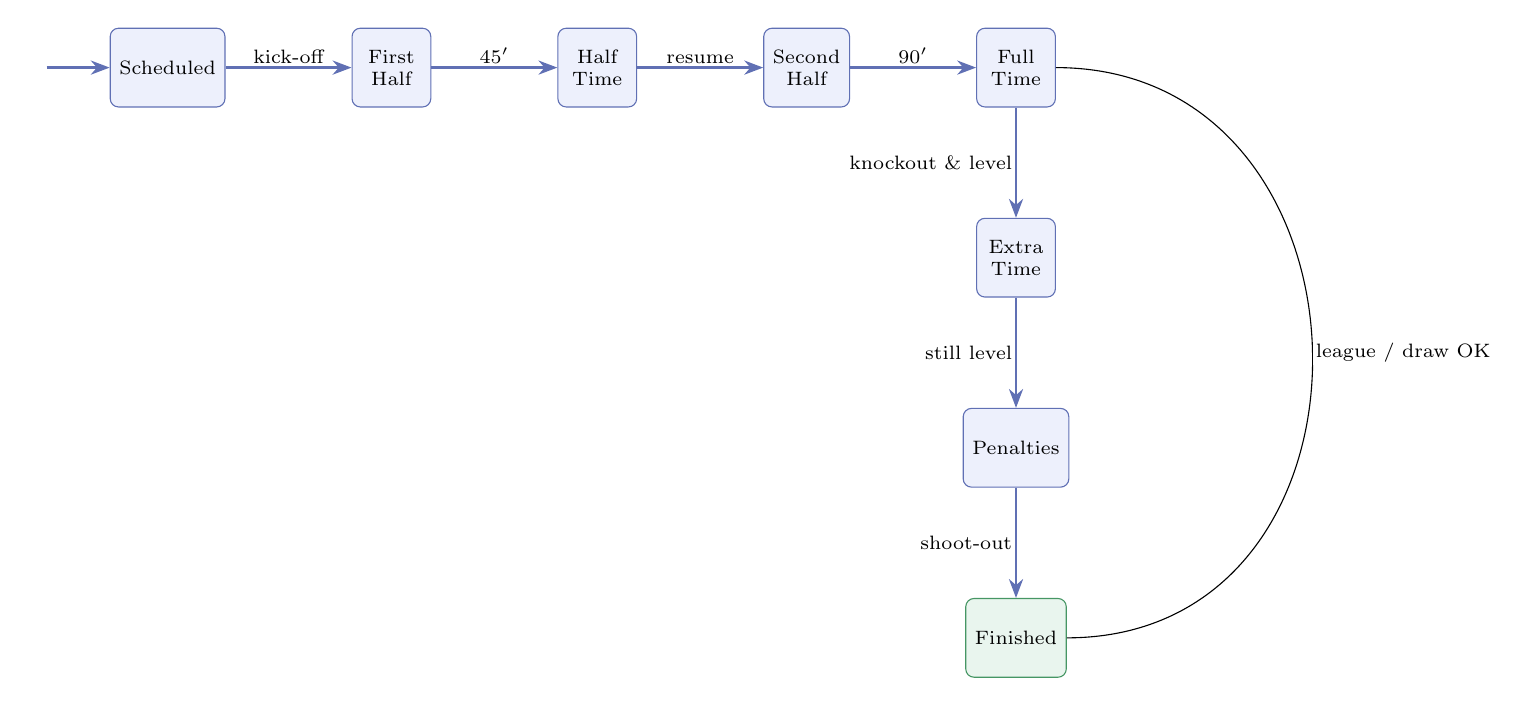
\begin{tikzpicture}[node distance=14mm and 16mm,
    every edge/.style={draw=dLine,thick,-{Stealth[length=2.4mm]}}]
  \node (start) {};
  \node[stbox, right=8mm of start] (sch) {Scheduled};
  \node[stbox, right=of sch] (h1) {First\\Half};
  \node[stbox, right=of h1]  (ht) {Half\\Time};
  \node[stbox, right=of ht]  (h2) {Second\\Half};
  \node[stbox, right=of h2]  (ft) {Full\\Time};
  \node[stbox, below=14mm of ft]  (et)  {Extra\\Time};
  \node[stbox, below=14mm of et]  (pen) {Penalties};
  \node[stbox, below=14mm of pen, fill=dFill2, draw=dLine2] (fin) {Finished};
  \draw (start) edge (sch);
  \draw (sch) edge node[lbl,above]{kick-off} (h1);
  \draw (h1)  edge node[lbl,above]{45$'$} (ht);
  \draw (ht)  edge node[lbl,above]{resume} (h2);
  \draw (h2)  edge node[lbl,above]{90$'$} (ft);
  \draw (ft)  edge node[lbl,left]{knockout \& level} (et);
  \draw (et)  edge node[lbl,left]{still level} (pen);
  \draw (pen) edge node[lbl,left]{shoot-out} (fin);
  \draw (ft)  to[out=0,in=0,looseness=1.5] node[lbl,right]{league / draw OK} (fin);
\end{tikzpicture}%
}
\caption{State machine for live-match phase progression, where a scheduled match advances through the regulation halves to full time and, for an unresolved knockout tie only, continues into extra time and a penalty shoot-out before finishing.}
\label{fig-state-match}
\end{figure}

% auto-generated figure: state-injury (source: fix)
\begin{figure}[H]
\centering
\resizebox{\textwidth}{!}{%
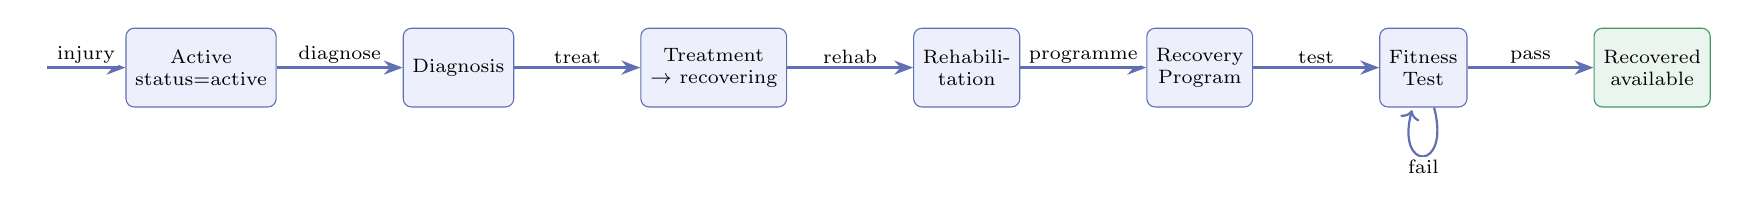
\begin{tikzpicture}[every edge/.style={draw=dLine,thick,-{Stealth[length=2.4mm]}}]
  \node (start) {};
  \node[stbox, right=10mm of start] (act)  {Active\\\scriptsize status=active};
  \node[stbox, right=16mm of act]   (diag) {Diagnosis};
  \node[stbox, right=16mm of diag]  (treat){Treatment\\\scriptsize $\rightarrow$ recovering};
  \node[stbox, right=16mm of treat] (rehab){Rehabili-\\tation};
  \node[stbox, right=16mm of rehab] (prog) {Recovery\\Program};
  \node[stbox, right=16mm of prog]  (fit)  {Fitness\\Test};
  \node[stbox, right=16mm of fit, fill=dFill2, draw=dLine2] (recd) {Recovered\\\scriptsize available};
  \draw (start) edge node[lbl,above]{injury} (act);
  \draw (act)   edge node[lbl,above]{diagnose} (diag);
  \draw (diag)  edge node[lbl,above]{treat} (treat);
  \draw (treat) edge node[lbl,above]{rehab} (rehab);
  \draw (rehab) edge node[lbl,above]{programme} (prog);
  \draw (prog)  edge node[lbl,above]{test} (fit);
  \draw (fit)   edge node[lbl,above]{pass} (recd);
  \draw (fit)   edge[loop below] node[lbl,below]{fail} (fit);
\end{tikzpicture}%
}
\caption{State machine for the injury lifecycle and recovery journey: the Injury.status field drives Active to Recovering to Recovered, with the staged journey (Diagnosis, Treatment, Rehabilitation, Recovery Program, Fitness Test) walked along the transitions, a failed fitness test looping back and a passed test restoring the player to Available.}
\label{fig-state-injury}
\end{figure}

% auto-generated figure: state-competition (source: wf)
\begin{figure}[H]
\centering
\resizebox{\textwidth}{!}{%
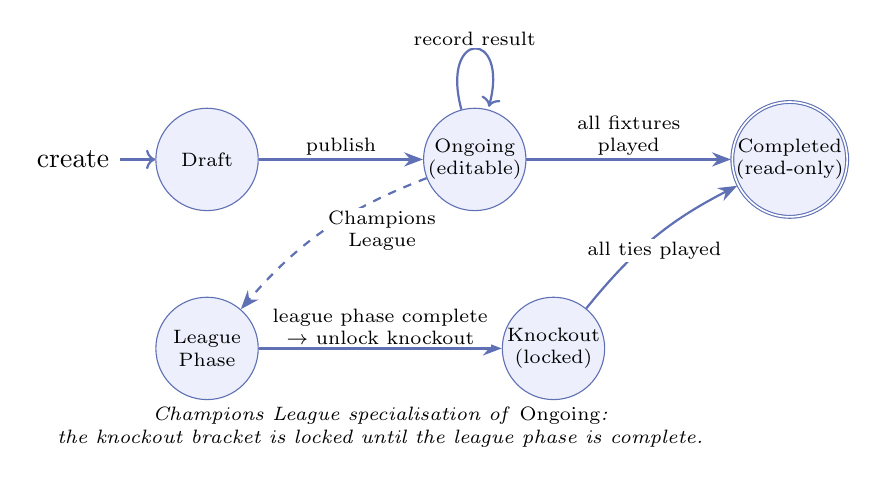
\begin{tikzpicture}[node distance=26mm, on grid,
    every edge/.style={flow,draw}]
  % --- main competition lifecycle ---
  \node[st,initial,initial text=create] (draft) {Draft};
  \node[st,right=34mm of draft]         (ongo)  {Ongoing\\(editable)};
  \node[st,accepting,right=40mm of ongo](comp)  {Completed\\(read-only)};

  \draw[flow] (draft) edge node[lbl,above]{publish} (ongo);
  \draw[flow] (ongo)  edge node[lbl,above,align=center]{all fixtures\\played} (comp);
  \draw[flow] (ongo)  edge[loop above] node[lbl]{record result} (ongo);

  % --- Champions League sub-states (knockout gated by league phase) ---
  \node[st,below=24mm of draft] (league) {League\\Phase};
  \node[st,right=44mm of league] (knock) {Knockout\\(locked)};

  \draw[flow] (league) edge node[lbl,above,align=center]{league phase complete\\$\rightarrow$ unlock knockout} (knock);
  \draw[flow] (knock)  edge[bend left=12] node[lbl,below,align=center]{all ties played} (comp);

  % link the CL specialisation to the generic Ongoing state
  \draw[flowd] (ongo) edge[bend right=14] node[lbl,right,align=center]{Champions\\League} (league);

  \node[font=\scriptsize\itshape,below=10mm of league,xshift=22mm,align=center]
    {Champions League specialisation of \emph{Ongoing}:\\the knockout bracket is locked until the league phase is complete.};
\end{tikzpicture}}
\caption{State machine for the competition lifecycle: a competition moves from Draft through an editable Ongoing phase to a read-only Completed state once every fixture is played, with the Champions League specialisation in which the knockout bracket stays locked until the league phase is complete.}
\label{fig-state-competition}
\end{figure}


\chapter{Results and Analysis}
\label{ch:results}

This chapter presents the implemented system and demonstrates, feature by feature,
how the requirements specified in Chapter~3 were realised in working software. Where
the preceding chapters reasoned about the system in the abstract---its architecture,
its data model and its planned behaviour---this chapter reports on the concrete
artefact that was built, deployed and exercised. The discussion follows the user's
journey through the deployed product---branded \textit{Sportify}---beginning with
onboarding and authentication, proceeding through the club, squad, competition and
match domains, and concluding with the medical, communication, analytics and
configuration modules. Each module is described along four consistent axes so that the
reader can move from \emph{intent} to \emph{mechanism} without losing the thread:
\begin{enumerate}
  \item the \emph{purpose} of the feature and the \emph{user experience} it delivers,
        illustrated by a screenshot of the running application;
  \item the \emph{back-end realisation}---which of the six Spring Boot
        microservices~\cite{springboot,microservices} owns the behaviour, the REST
        endpoints it exposes through the Spring Cloud Gateway~\cite{springcloud}, and
        the JPA entities and database tables that persist its state~\cite{postgres};
  \item the \emph{key logic and algorithms} in genuine detail---the fixture-generation
        routines, the standings recomputation, the live-match phase machine, the
        per-sport substitution rules, the in-match injury bridge, the status-driven
        medical workflow, the chat group/invitation model and WebSocket
        protocol~\cite{websocket}, the event-driven notification pipeline, the
        three-layer enforcement of role-based access~\cite{rbac}, and the Keycloak
        password re-verification~\cite{keycloak,jwt}; and
  \item the \emph{validation and edge-case handling} that makes each feature robust in
        the face of stale data, partial input and concurrent operation.
\end{enumerate}
The front-end is a Next.js~16 / React~19 application~\cite{nextjs,react} that talks to
the back-end exclusively through a single gateway origin, and every state-changing
action is persisted server-side so that a browser reload faithfully reconstructs the
application state. A substantial analytical discussion at the end of the chapter
(Section~\ref{sec:res-analysis}) evaluates how completely the delivered system
satisfies the functional and non-functional requirements, reports performance and
user-experience observations, and describes the testing approach that was followed.

%======================================================================
\section{Onboarding and Authentication}
\label{sec:res-login}

The entry point to the platform is a single sign-in surface that delegates identity
to Keycloak~\cite{keycloak}, the system's dedicated OpenID Connect identity provider.
Rather than implement its own credential store---an approach that would scatter
password hashing, lockout policy and token issuance across the domain services---the
platform treats identity as a cross-cutting concern owned by a purpose-built provider,
which is one of the architectural decisions defended in Chapter~3.

\paragraph{User experience.} A user submits a username and password on the sign-in
screen (Figure~\ref{fig:login}). On success the user is taken directly to the
operational home of the product; on failure a concise, non-revealing error is shown.
There is deliberately no separate landing page per role: every authenticated user
arrives at the single \texttt{/dashboard} route, whose contents are then computed from
the resolved role so that the same URL renders a different, permission-appropriate
surface for each user.

\paragraph{Back-end realisation.} The credentials are posted to the gateway, which
performs the OAuth~2.0 Resource Owner Password Credentials grant against the
\texttt{mscms} realm. Keycloak validates the credentials and returns a signed JSON Web
Token~\cite{jwt}. The token is the only proof of identity the rest of the system
trusts: every subsequent request carries it as a bearer token, the gateway validates
its signature and expiry before forwarding the request, and each microservice reads the
claims to authorise the operation. The user-management service (port~8081) brokers the
administrative side of identity---creating Keycloak users, assigning realm and client
roles, and reconciling the local user profile with the identity provider---through a
\texttt{KeycloakAdminService} that itself obtains a short-lived admin token from the
\texttt{master} realm before each privileged call.

\paragraph{Key logic.} The front-end decodes the \texttt{access\_token} client-side and
extracts two pieces of information. The token's \texttt{sub} claim is persisted as the
\texttt{keycloakId}---the canonical, stable identity used throughout the system, never
an internal database primary key, so that a service can correlate a player, a chat
member and an alert recipient without sharing a relational schema. The resolved role is
stored both in \texttt{localStorage}, where the API client reads it, and as a cookie
that the Next.js middleware reads on the server side to guard routes before a page is
ever rendered~\cite{rbac}. This dual storage is what makes the three-layer access
scheme described in Chapter~3 effective on the client tier: the cookie protects
navigation, while the token protects the API.

\paragraph{Validation and recovery.} Should a request later fail with HTTP~401---for
example after a token has expired, or after a database re-seed has invalidated the
previously issued token---the shared API client intercepts the response, clears local
storage and redirects the user transparently back to the login screen. This converts
what would otherwise be a confusing sequence of silently failing requests into a clean,
self-healing recovery path, and it guarantees that the application never operates in a
half-authenticated state.

\begin{figure}[htbp]
  \centering
  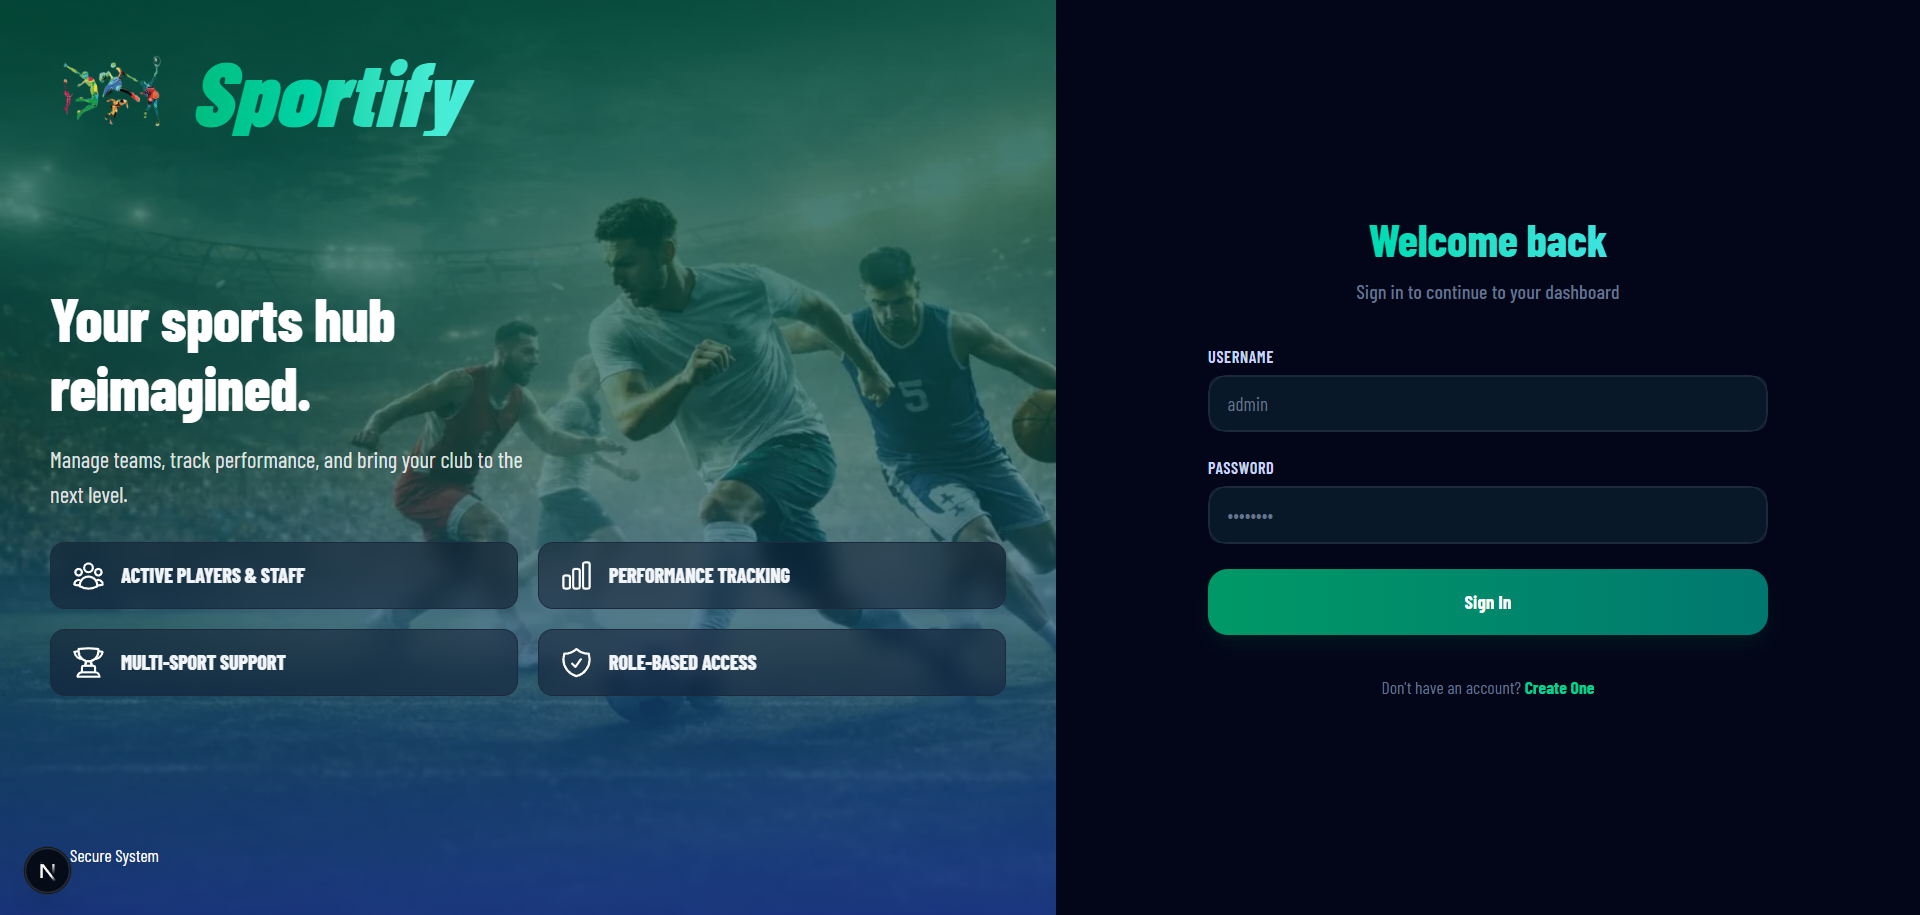
\includegraphics[width=0.85\textwidth]{fig-login.png}
  \caption{The Sportify sign-in screen. Credentials are validated against the Keycloak
  \texttt{mscms} realm through the API gateway, which returns a signed JWT that the
  front-end decodes to establish the user's identity and role.}
  \label{fig:login}
\end{figure}

%======================================================================
\section{Role-Aware Dashboard}
\label{sec:res-dashboard}

After authentication the user is presented with a unified dashboard that acts as the
operational home of the platform. The design intent is that a member of staff should be
able to assess the state of the club in a single glance, without first deciding which
of a dozen modules to open.

\paragraph{User experience.} Rather than maintaining a separate landing page per role,
the dashboard is assembled dynamically (Figure~\ref{fig:dashboard}). It composes a hero
banner carrying the club identity, a featured upcoming or most-recent match, a condensed
La~Liga standings strip, and a set of summary cards---squad size, scheduled matches,
active injuries and unread alerts---whose visibility is filtered by the permission
map~\cite{rbac}. A medical doctor and a sponsor consequently see overlapping but
distinct sets of cards, even though both navigated to the identical URL.

\paragraph{Back-end realisation.} The dashboard is a true aggregation surface: it has no
dedicated back-end of its own, but instead composes data fetched from several
microservices through the gateway on a single origin. Player counts are read from the
player-management service (port~8084), fixtures and live status from the training-match
service (port~8087), medical figures from the medical-fitness service (port~8086), and
unread-alert counts from the notification-mail service (port~8085). The fetch-based API
client issues these requests in parallel and the React layer composes the responses,
which keeps the perceived latency close to that of the slowest single call rather than
the sum of all of them.

\paragraph{Key logic and resilience.} Because the dashboard depends on several
independent services, it is designed to degrade gracefully: each summary card resolves
independently, so a momentarily unavailable medical service suppresses only the injuries
figure rather than blanking the whole page. The featured-match selection logic prefers
the next scheduled match and falls back to the most recent completed one, ensuring the
hero area is never empty even outside the playing season. This combination of parallel
aggregation and per-card isolation gives every member of staff an immediate,
role-appropriate and fault-tolerant snapshot of club operations on entry.

\begin{figure}[htbp]
  \centering
  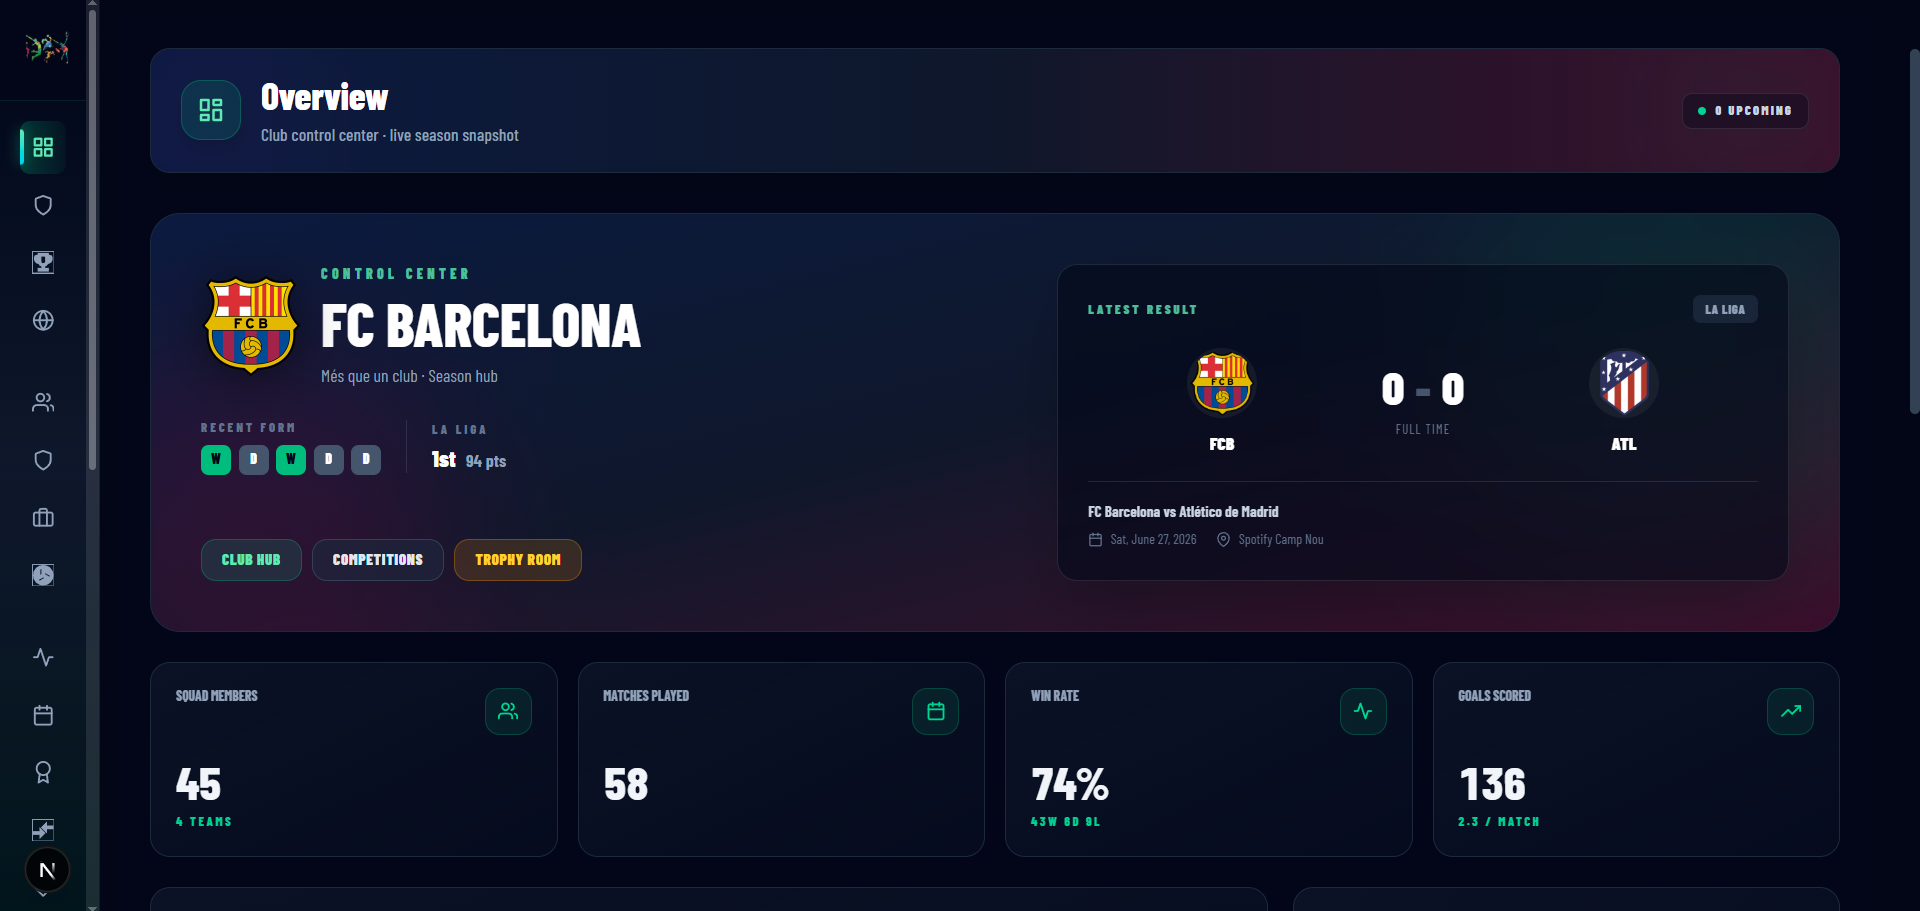
\includegraphics[width=0.95\textwidth]{fig-dashboard.png}
  \caption{The role-aware dashboard. Summary cards, a featured match and a mini league
  table aggregate data from multiple microservices into a single overview surface, with
  card visibility governed by the user's role.}
  \label{fig:dashboard}
\end{figure}

%======================================================================
\section{Club Hub}
\label{sec:res-clubhub}

The Club Hub consolidates the modelled club's institutional identity into a single page.
Where the dashboard answers ``what is happening right now?'', the Club Hub answers ``who
are we?'', presenting the club as a continuous sporting institution rather than a set of
disconnected records.

\paragraph{User experience.} Taking FC~Barcelona as the working example, the Club Hub
presents the club crest and colours, the head coach, the home stadium, a trophy cabinet,
and the full squad rendered as player cards with real photographs
(Figure~\ref{fig:club-hub}). Crucially, the page also surfaces \emph{live} sporting
context rather than a static brochure: recent results are grouped by competition, a
``last-five'' form strip summarises momentum at a glance using a colour-coded
win/draw/loss sequence, and a \texttt{LIVE} badge appears whenever a match is in
progress.

\paragraph{Back-end realisation and the single-source-of-truth principle.} All of the
sporting data on this page originates from the back-end, which is the single source of
truth---the front-end never contacts the external football data provider directly. This
is a deliberate architectural constraint with several payoffs: the API key is never
exposed to the browser, the provider's rate limits are governed centrally, and the data
the user sees is exactly the data the rest of the system reasons about. Concretely, the
training-match service ingests fixtures and results on a schedule (see
Section~\ref{sec:res-laliga}) and the Club Hub reads the consolidated \texttt{Match}
records through the gateway, joining them client-side into the per-competition groupings
and the form strip.

\paragraph{Edge cases.} Because the modelled system date sits after the conclusion of
the imported seasons, the ``live'' badge and ``upcoming'' groupings are written to behave
correctly in the absence as well as the presence of in-progress matches: when no match is
live the badge is simply omitted, and when no fixtures remain the recent-results view is
shown in its place, so the page is always coherent regardless of where in the season the
club currently sits.

\begin{figure}[htbp]
  \centering
  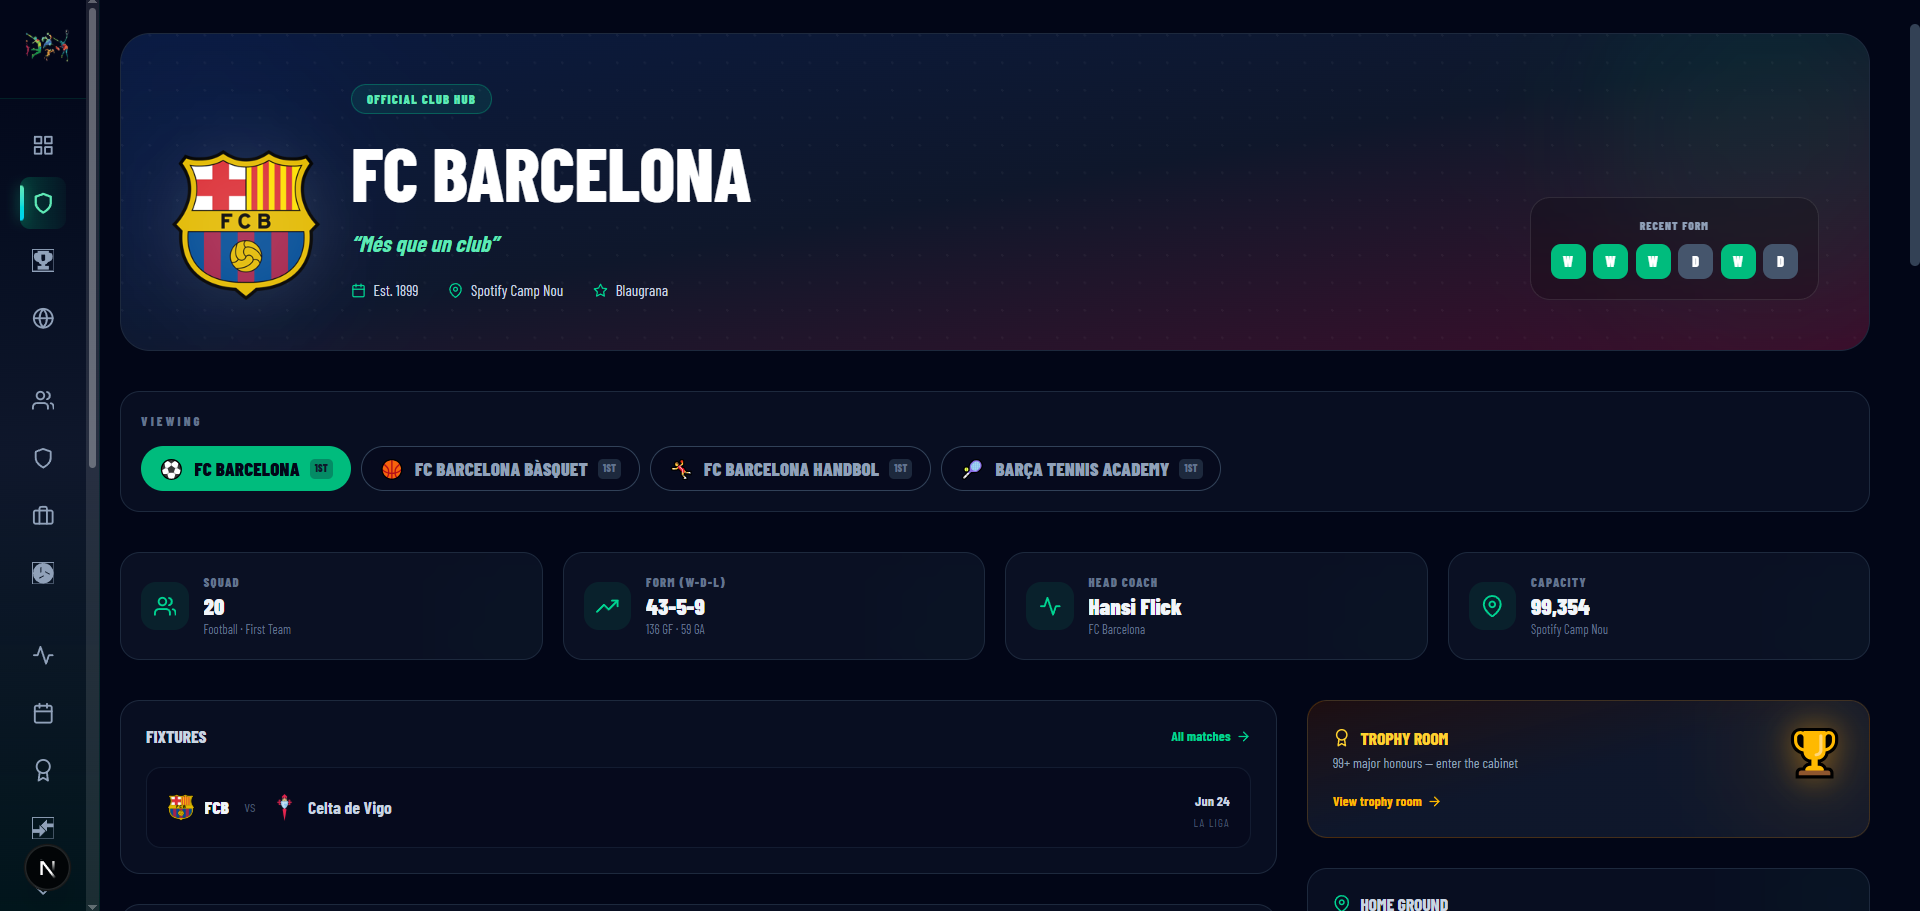
\includegraphics[width=0.95\textwidth]{fig-club-hub.png}
  \caption{The Club Hub, presenting club identity, coaching and stadium details, the
  trophy cabinet, the squad, and results grouped by competition with a last-five form
  strip.}
  \label{fig:club-hub}
\end{figure}

%======================================================================
\section{Squad and Player Profiles}
\label{sec:res-players}

The Players module manages the multi-sport roster maintained by the player-management
service (port~8084). It is the module that most directly demonstrates the platform's
multi-discipline ambition.

\paragraph{User experience.} Players are listed as cards filterable by sport and
availability status, each carrying a real photograph, position and headline details
(Figure~\ref{fig:players}). Selecting a card opens an expanded detail view with the
player's biography, contract data and statistics, presented with a subtle ball-roll
animation that gives the transition a polished, product-quality feel
(Figure~\ref{fig:player-detail}).

\paragraph{Back-end realisation and data model.} Each player is a \texttt{Player} entity
keyed internally by a numeric identifier but correlated to identity by a
\texttt{keycloakId}, so the same person can be a squad member here, a chat participant in
the messaging service and an alert recipient in the notification service without any of
those services sharing a database. The entity carries a \texttt{photoUrl} populated from
public reference images, a \texttt{status} field (for example \texttt{AVAILABLE} or
\texttt{INJURED}), a \texttt{sportType} discriminator and the position and attribute
fields appropriate to the player's discipline. The module exposes the conventional REST
surface for listing, retrieving, creating and updating players, plus a dedicated
status-mutation endpoint that the live-match engine and the medical module call to flip a
player between availability states (Sections~\ref{sec:res-live}
and~\ref{sec:res-medical}).

\paragraph{Key logic.} Because the underlying model is sport-aware, the same listing
transparently accommodates footballers, basketballers, handball and tennis players, each
with the positions and attributes appropriate to their discipline, which directly
satisfies the multi-discipline requirement established in Chapter~2. The
\texttt{status} field is consumed across the platform as the authoritative statement of a
player's availability: a player marked \texttt{INJURED} is filtered out of lineup pickers,
match selection and training attendance automatically, which is what allows the medical
workflow to withdraw a player from operations simply by changing one field rather than by
editing every dependent module.

\begin{figure}[htbp]
  \centering
  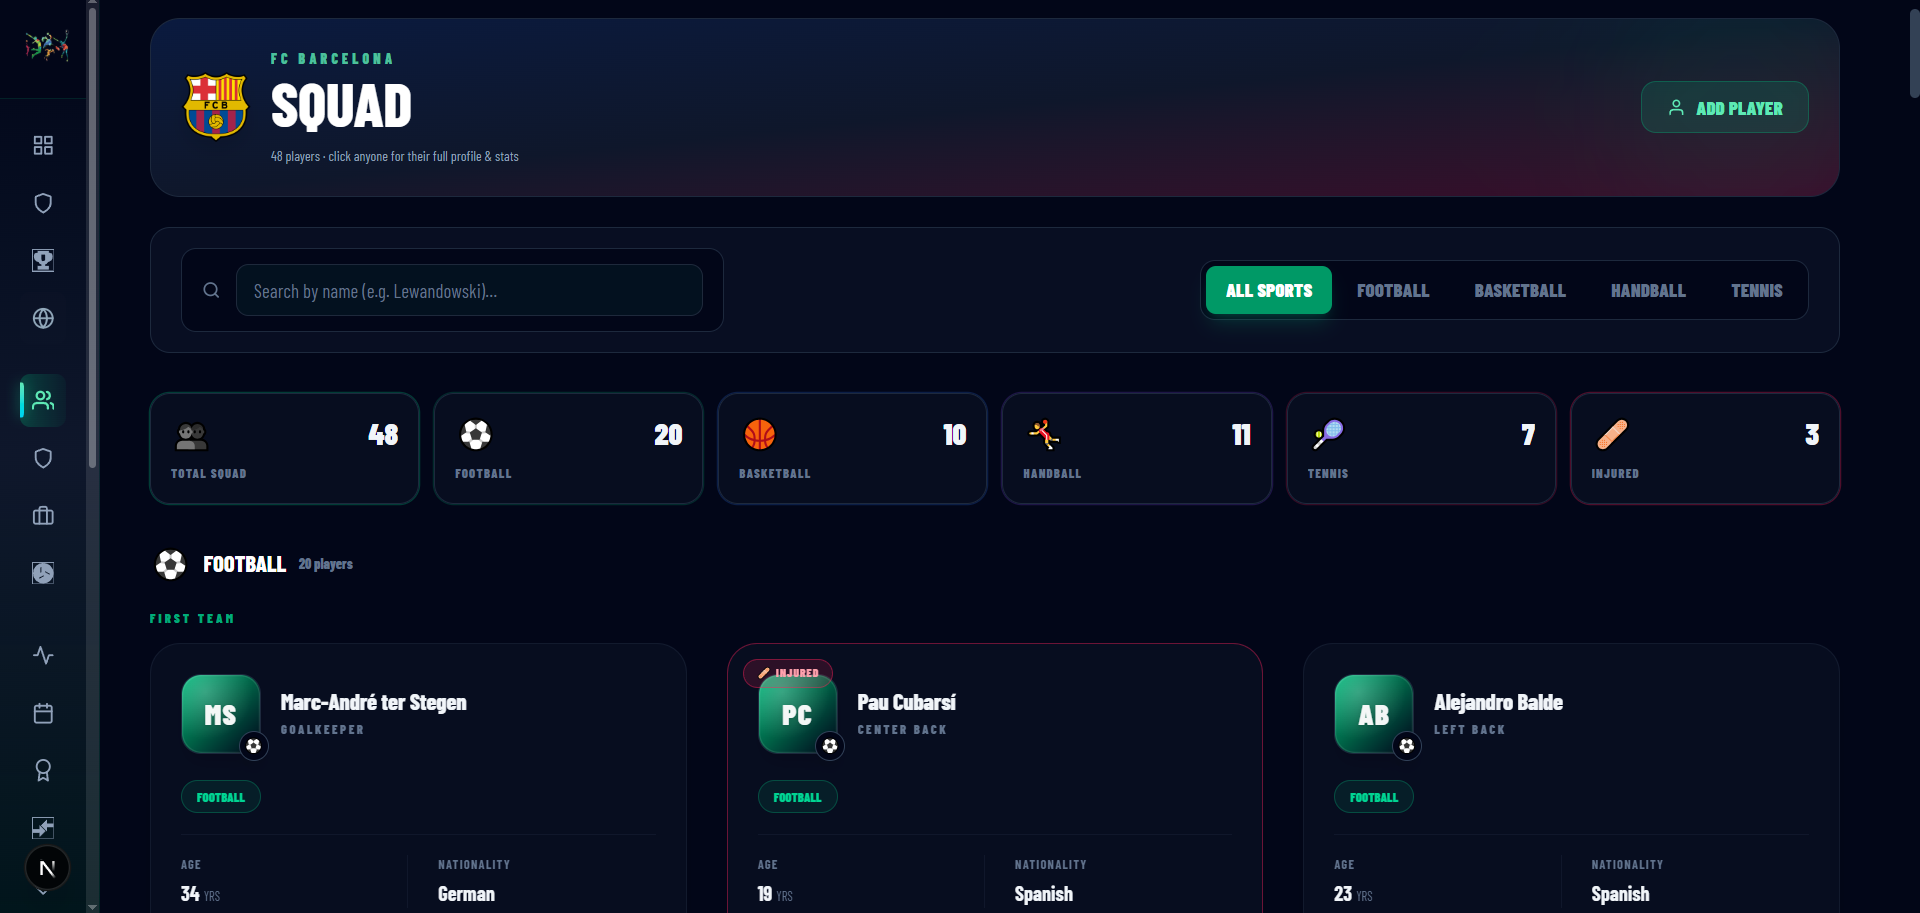
\includegraphics[width=0.95\textwidth]{fig-players.png}
  \caption{The squad listing. Players are rendered as photograph-bearing cards,
  filterable by sport and availability, and served by the player-management service.}
  \label{fig:players}
\end{figure}

\begin{figure}[htbp]
  \centering
  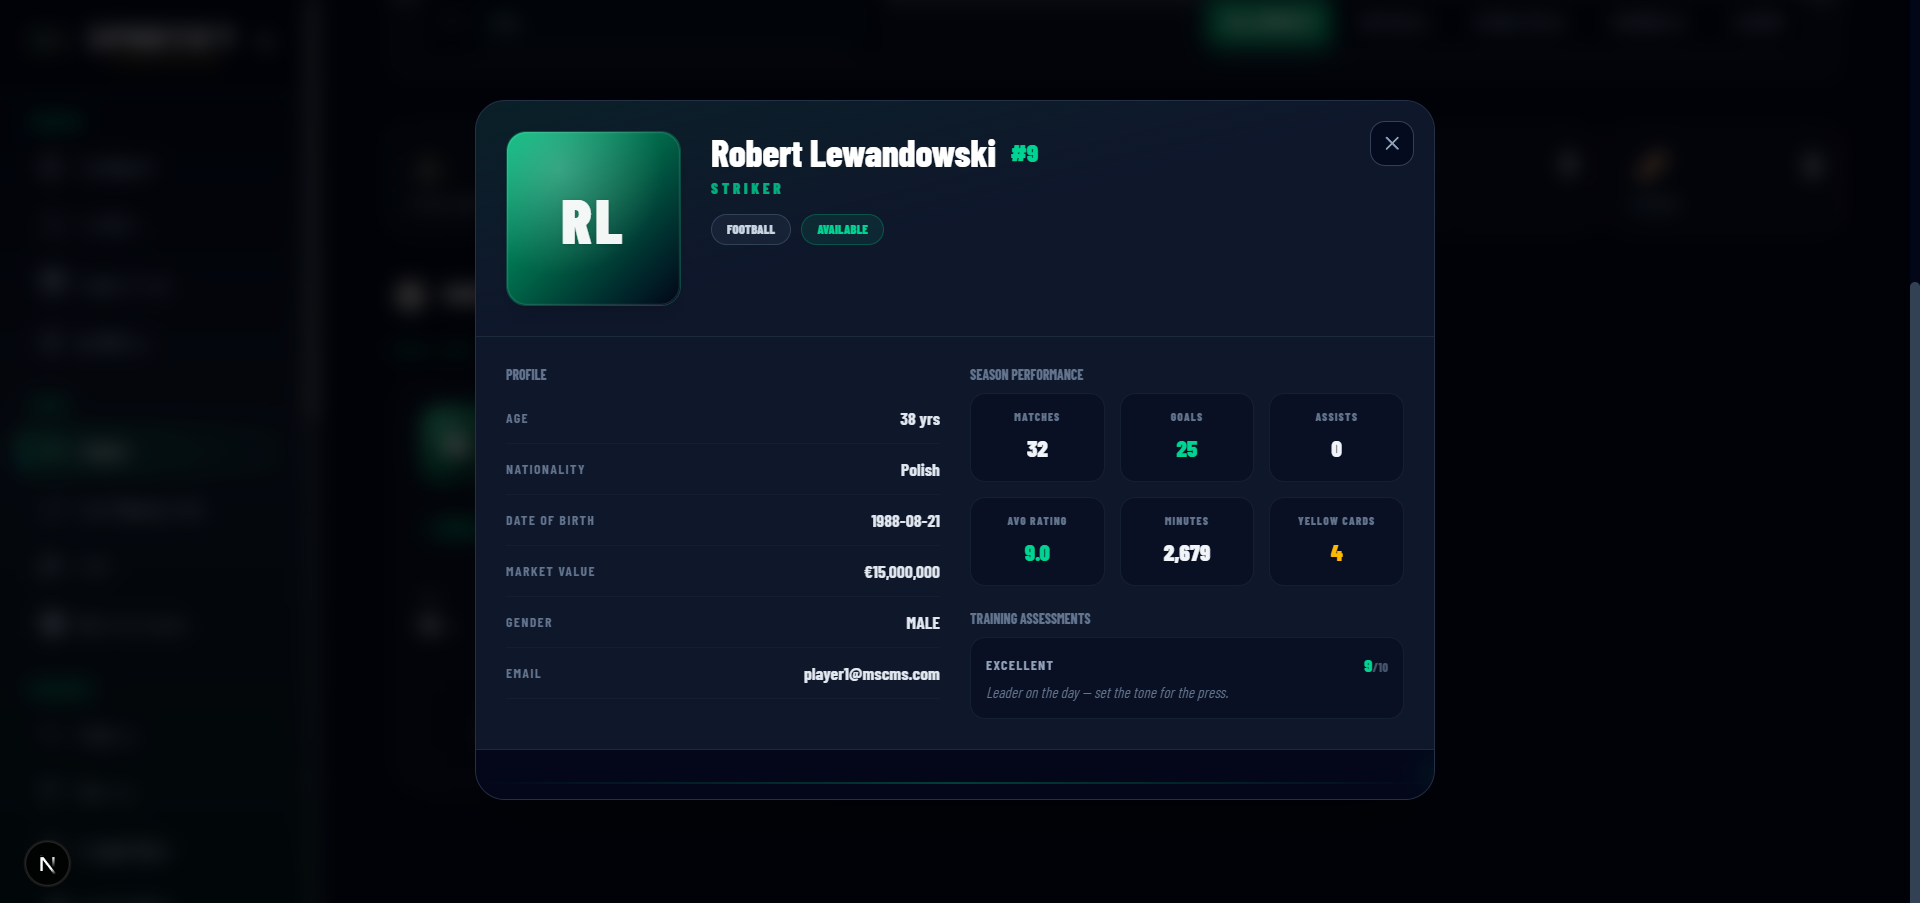
\includegraphics[width=0.8\textwidth]{fig-player-detail.png}
  \caption{The expanded player profile, showing biography, contract and statistics for an
  individual squad member, opened with a subtle animation from the squad listing.}
  \label{fig:player-detail}
\end{figure}

%======================================================================
\section{Competitions}
\label{sec:res-competitions}

Competitions are modelled as first-class, database-backed entities owned by the
training-match service, in contrast to the throwaway, in-memory league tables of a
typical demonstration application. This decision is what allows the platform to enforce
realistic competition rules, to recompute standings deterministically, and to write live
results back to an authoritative fixture.

\paragraph{Data model.} Three persistent JPA entities capture the domain.
\texttt{Competition} records the competition's name, season, \texttt{type}
(\texttt{LEAGUE} or a knockout-style type) and the number of \texttt{rounds} a league
plays. \texttt{CompetitionTeam} records each participating team---its name, short name,
crest URL and sport---scoped to a competition. \texttt{CompetitionFixture} records a
single fixture: the home and away team identities and names, an optional \texttt{round}
label (empty for a plain league fixture, \texttt{LEAGUE\_STAGE} or a knockout label such
as \texttt{R16} otherwise), a \texttt{matchday} bucket, a \texttt{played} flag, the
recorded scores, and the timestamp at which the result was entered. These three entities
are exposed through a single controller mounted under \texttt{/matches/leagues} so that
no additional gateway route is required---the existing route to the training-match service
is reused, which keeps the gateway configuration small and auditable.

\paragraph{Scope and user experience.} The platform deliberately scopes football
competitions to the two that mirror the club's real calendar: \emph{La~Liga} (Spain's
Primera Divisi\'on, which the system treats as one and the same competition rather than
duplicating it) and the \emph{UEFA Champions League}. The Competitions landing page
presents these as selectable tabs and acts as the gateway into each competition's detailed
view (Figure~\ref{fig:competitions}). Real, completed seasons were imported as seed data
through a dedicated \texttt{/matches/leagues/import} endpoint that reads a season's matches
from the provider and materialises a competition, its teams and every finished fixture in
one transaction.

\paragraph{The read-only completed-competition rule.} A deliberate design decision marks
any competition whose every fixture has been played as \emph{read-only}: such a
competition displays a ``Completed---read-only'' badge and forbids result or date edits,
while an ongoing competition remains editable until its final result is recorded, at which
point it locks automatically. This rule exists to protect the integrity of historical
records---a finished season is a fact, not a draft---while still permitting an in-progress
competition to be updated match by match. Administrative deletion remains available in all
cases, since removing an entire competition is a coarse, intentional act rather than an
accidental edit.

\begin{figure}[htbp]
  \centering
  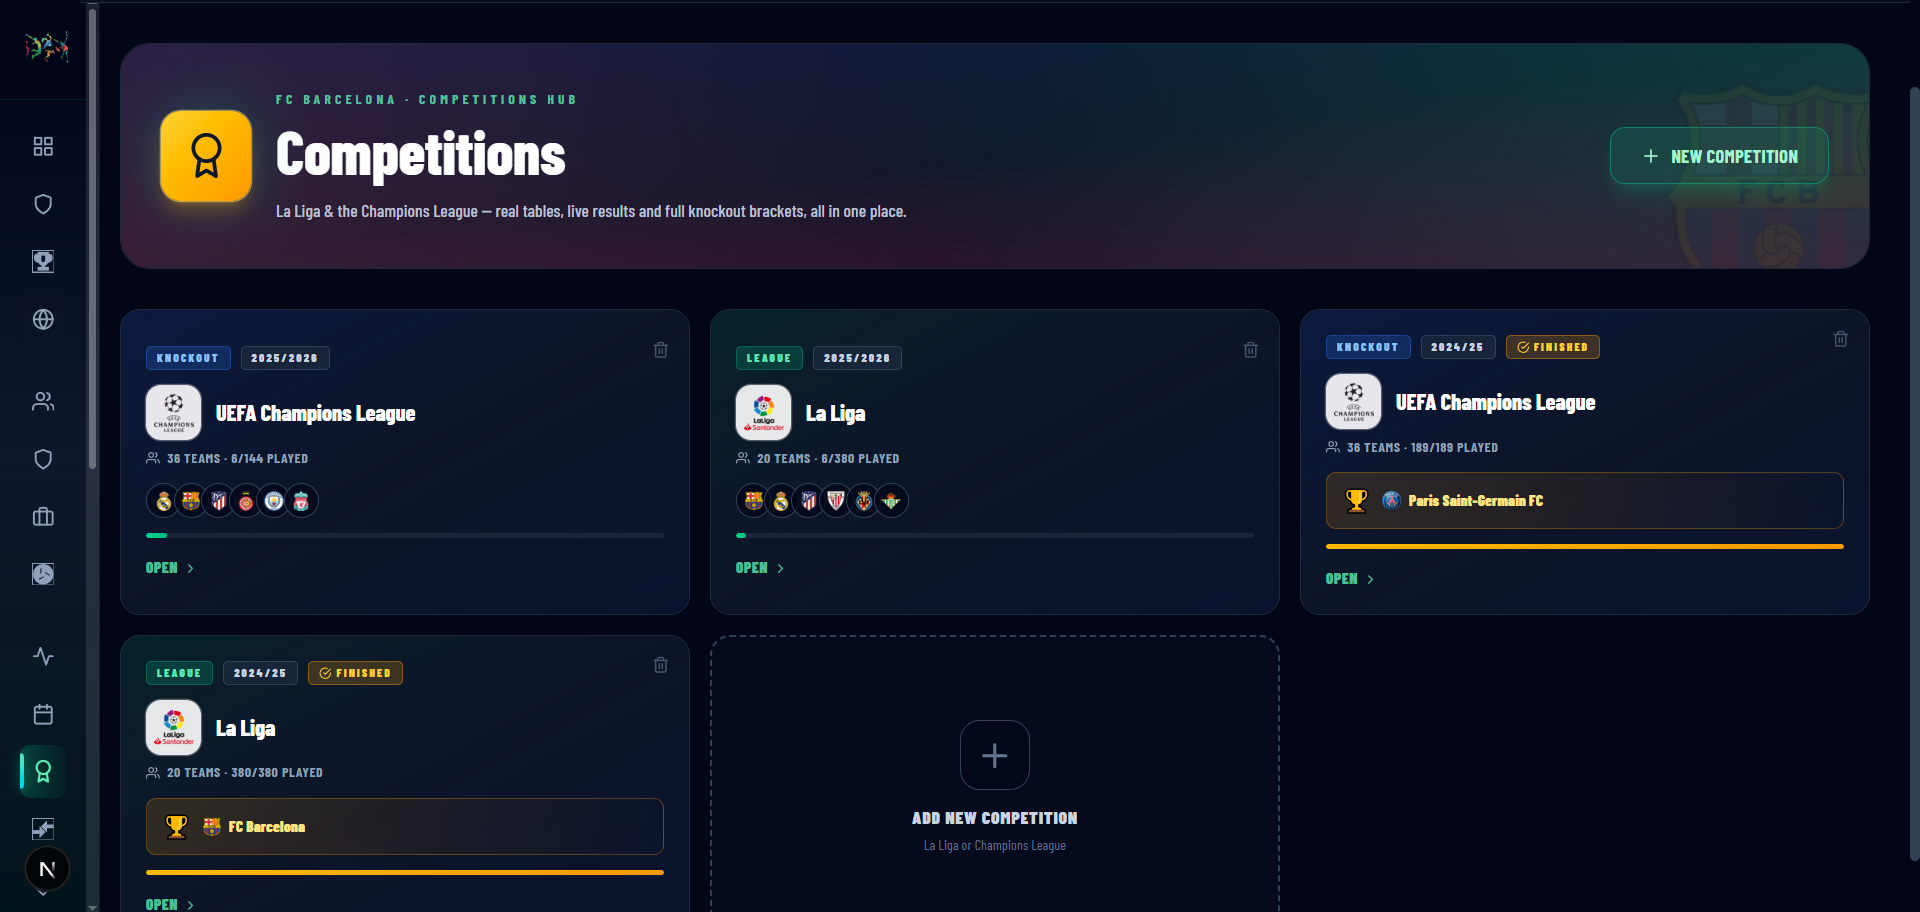
\includegraphics[width=0.95\textwidth]{fig-competitions.png}
  \caption{The Competitions landing page, with selectable tabs for La~Liga and the UEFA
  Champions League backed by persistent competition entities.}
  \label{fig:competitions}
\end{figure}

\subsection{La~Liga: Standings and Fixtures}
\label{sec:res-laliga}

The La~Liga view renders a live standings table together with the fixture and results
list for the season (Figure~\ref{fig:laliga}).

\paragraph{Standings computation.} The standings are not stored; they are recomputed from
the fixtures on every read, which guarantees they can never drift out of sync with the
underlying results. The computation iterates over the played fixtures, and for each one
credits three points to a win, one to each side of a draw, and zero to a loss, while
accumulating goals for, goals against and the played/won/drawn/lost tallies. The resulting
rows are then ordered by points, then by goal difference, then by goals scored---the
ordering used by the real competition---so that recording a single result and reloading the
table produces exactly the movement a spectator would expect. Because the recomputation is a
pure function of the fixture set, it is deterministic and trivially testable.

\paragraph{Ingestion pipeline.} For fixtures that are still to be played, the data is kept
current through the training-match service's ingestion pipeline. A
\texttt{FootballDataClient} together with a \texttt{MatchSyncService} polls the
football-data.org provider~\cite{footballdata} on a thirty-minute schedule---implemented as
a Spring \texttt{@Scheduled} task with an initial delay of roughly twenty-five seconds after
boot and a configurable interval---and on demand through an administrative
\texttt{/matches/sync-external} endpoint. The service reads the configured competitions
(\texttt{PD} for La~Liga and \texttt{CL} for the Champions League), filters the modelled
club's fixtures by the club's provider team identifier, and upserts them into the local
\texttt{Match} table. Each fixture is de-duplicated by an \texttt{externalId} derived from the
provider's match identifier, so repeated synchronisation is idempotent and never produces
duplicates.

\paragraph{Working within the provider's constraints.} The free tier of the provider forbids
team-scoped endpoints---a request to \texttt{/teams/\{id\}/matches} is rejected---so the
service instead reads the permitted competition-scoped match and standings endpoints and
filters client-side for the modelled club. The competition standings are served through a
read-through pass exposed at \texttt{/matches/standings/\{code\}} that is never persisted,
so the live league position always reflects the provider's current figures without the
platform attempting to mirror data it does not own. This design keeps the back-end
authoritative for the data the platform manages while still presenting accurate, real-world
league context, and it respects the provider's terms by centralising every external call
behind the API key held only on the server.

\begin{figure}[htbp]
  \centering
  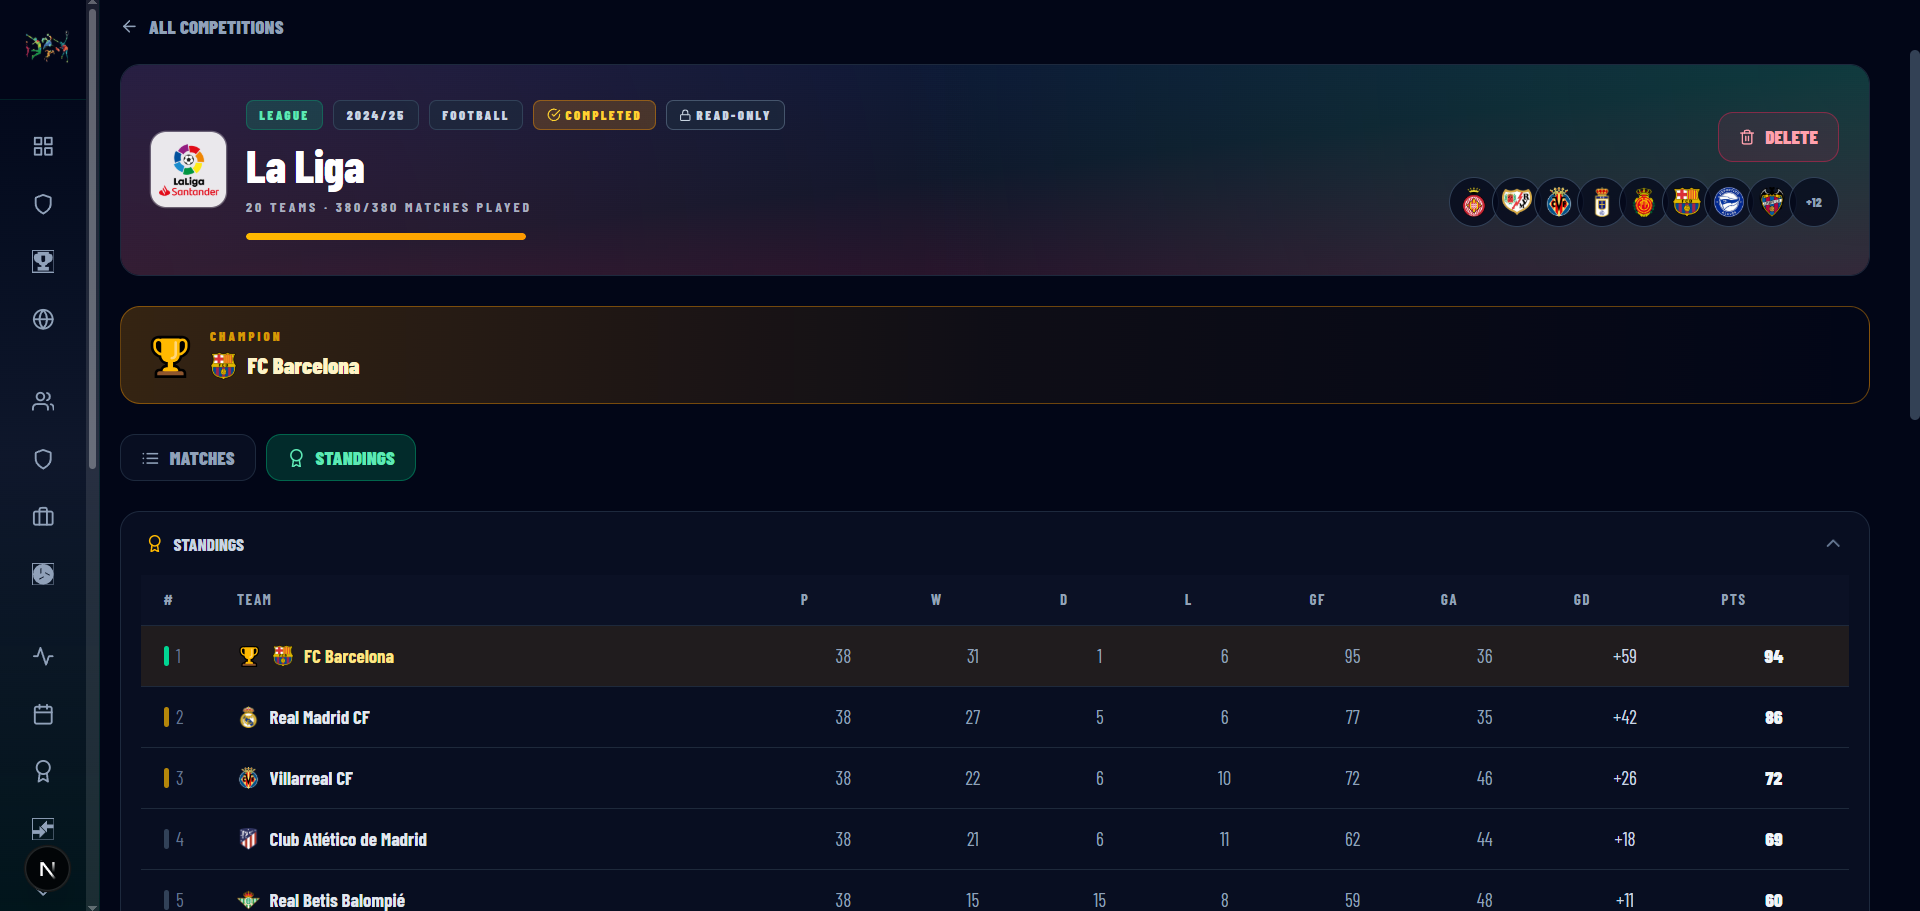
\includegraphics[width=0.95\textwidth]{fig-laliga.png}
  \caption{The La~Liga competition view, showing the live standings table alongside the
  season's fixtures and results.}
  \label{fig:laliga}
\end{figure}

\subsection{Champions League: League Phase and Knockout Bracket}
\label{sec:res-cl-bracket}

The Champions League view reproduces the competition's modern format with exactly two tabs
(Figure~\ref{fig:cl-bracket}). The first presents the single \emph{league phase}, in which
all thirty-six participating teams accumulate points in one combined table; the fixtures of
this stage are stored under a \texttt{LEAGUE\_STAGE} round so that the engine can distinguish
them from knockout ties. The second presents the \emph{knockout bracket}, rendered as a
progression of ties from the knockout play-off and round of sixteen through to the final. The
knockout tab remains locked until the league phase is complete, mirroring the real
competition's sequencing and preventing the user from advancing prematurely.

\paragraph{Why the round label matters.} The same \texttt{CompetitionFixture} model underpins
both stages, with each fixture's \texttt{round} value classifying it as either a points fixture
or a knockout tie. This single discriminator carries real behavioural weight: as
Section~\ref{sec:res-live} describes, the live-match engine consumes it to decide whether a
draw is a valid result. A league-phase fixture permits a draw and the engine stops at full
time; a knockout tie does not, and the engine extends into extra time and, if necessary, a
penalty shootout. Threading the format rule through one authoritative field, rather than
duplicating it in the user interface, is what keeps the live engine and the competition record
consistent.

\begin{figure}[htbp]
  \centering
  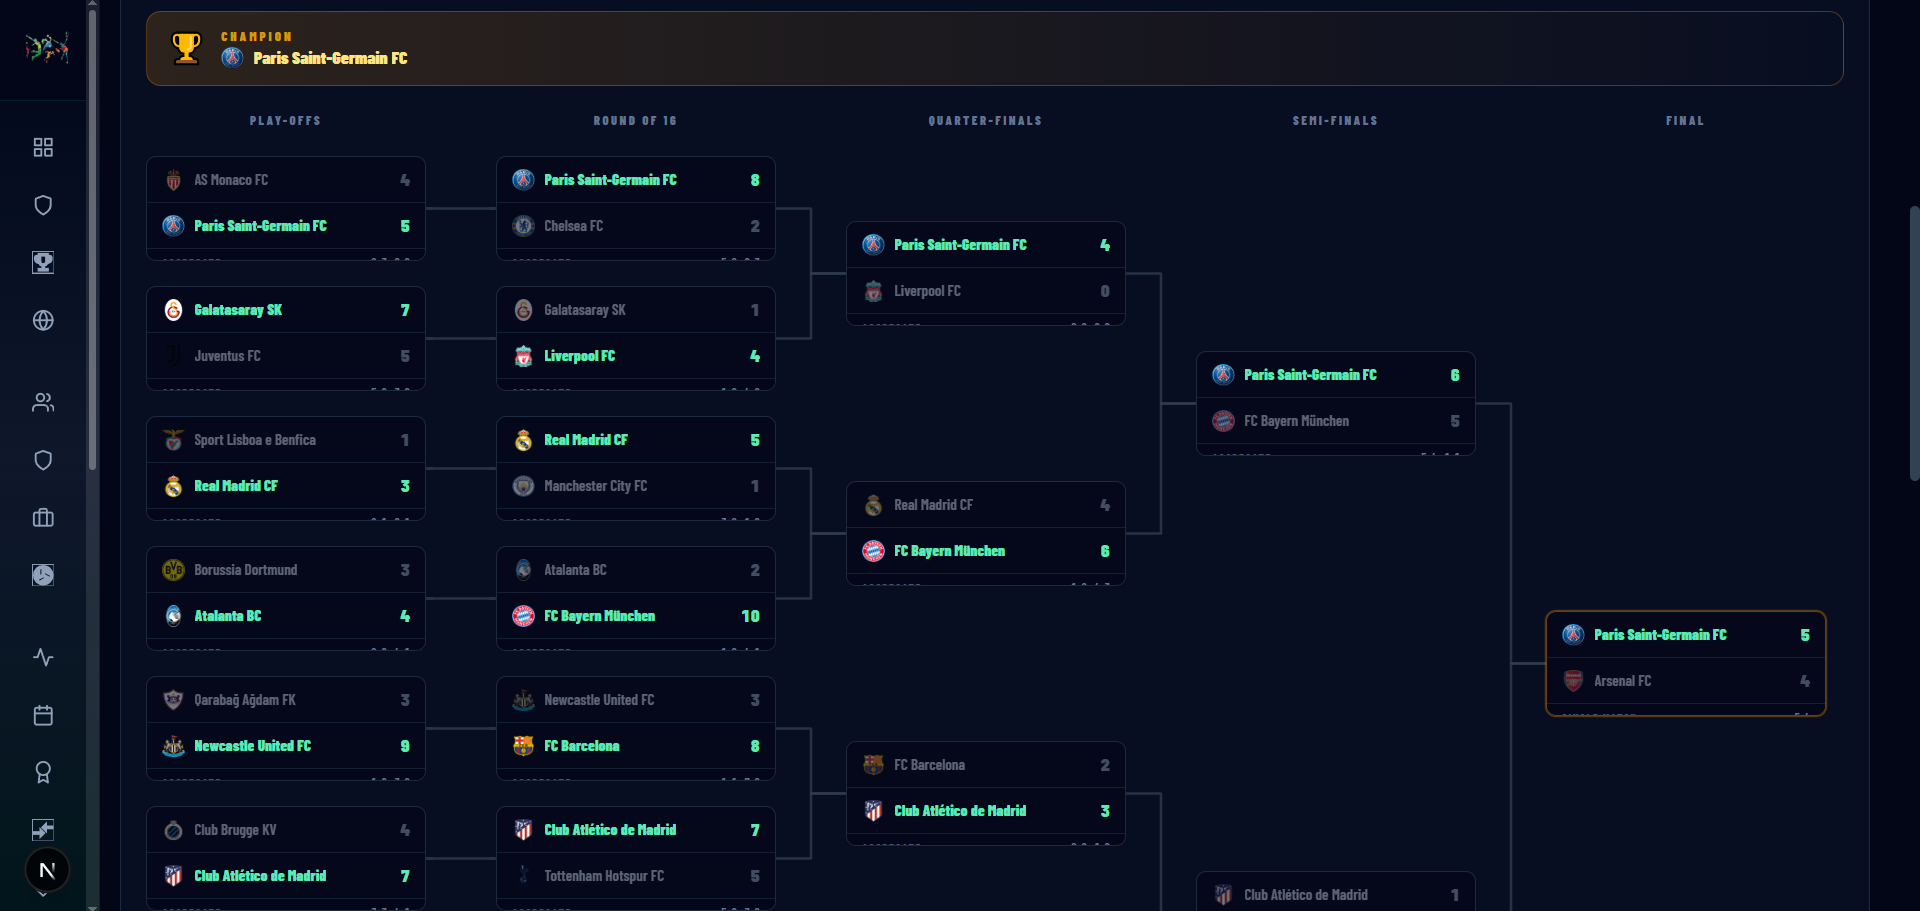
\includegraphics[width=0.95\textwidth]{fig-cl-bracket.png}
  \caption{The UEFA Champions League knockout bracket, presenting the progression of ties
  from the round of sixteen to the final. The bracket is unlocked only once the league
  phase has concluded.}
  \label{fig:cl-bracket}
\end{figure}

\subsection{Creating a Competition}
\label{sec:res-create-competition}

Administrators may author a new competition through a guided, multi-step flow
(Figure~\ref{fig:create-competition}). The user first selects a preset (La~Liga or
Champions League), then a season from a curated list, and finally the participating teams:
La~Liga is fixed at its twenty members, whereas the Champions League flow lets the
administrator select thirty-six clubs from a curated European team pool.

\paragraph{La~Liga generation: the double round-robin.} For a league competition the
back-end pre-generates the entire schedule on creation so that the user can only ever enter
results for genuine fixtures and can never inflate the table by recording the same pairing
repeatedly. The generator implements a double round-robin: it iterates over the configured
number of rounds (two for La~Liga) and, within each round, over every unordered pair of
teams, emitting one fixture per pair. The home and away sides are swapped on alternate rounds
so that each pairing is played once at home and once away, exactly as the real competition is
structured, and each fixture is assigned an incrementing \texttt{matchday} for display
grouping. For twenty teams this yields the expected $20 \times 19 = 380$ fixtures.

\paragraph{Champions League generation: the league-phase rotation algorithm.} The Champions
League league phase is the most algorithmically interesting case, because each of the
thirty-six teams must play exactly eight \emph{distinct} opponents---it is not a full
round-robin, in which every team would play every other. The platform generates this with a
deterministic circle/rotation pairing. The algorithm maintains, for every team, a running
\emph{degree} (the number of opponents already assigned) and a set of pair keys already used.
It then sweeps over rotational offsets: for an offset $o$ it considers pairing team $i$ with
team $(i + o) \bmod n$, and accepts the pairing only if both teams still have spare degree
and the unordered pair has not already been scheduled. Home and away are assigned by a parity
rule so that home counts stay balanced across the field. The sweep continues, increasing the
offset, until the total number of fixtures reaches $\tfrac{n \times 8}{2} = 144$, at which
point every team has exactly eight distinct opponents and no pairing is repeated. The
fixtures are then distributed across eight matchday buckets purely for display grouping, and
every fixture is tagged with the \texttt{LEAGUE\_STAGE} round so that it renders in the league
phase and is correctly treated as draw-permitting by the live engine. Because the algorithm is
deterministic, the same team list always produces the same regular, well-spread fixture graph,
which makes the generated schedule reproducible and verifiable.

\paragraph{Persistence and atomicity.} On confirmation the back-end generates the appropriate
fixture set---the round-robin for a league, or a bulk insert of the rotation-generated
league-phase fixtures for the Champions League via a \texttt{/matches/leagues/\{id\}/fixtures/bulk}
endpoint---and persists the competition together with its teams and fixtures inside a single
transaction. This converts what would traditionally be a manual, error-prone, spreadsheet-driven
exercise into one auditable, all-or-nothing operation: either the entire competition is created
correctly or none of it is.

\begin{figure}[htbp]
  \centering
  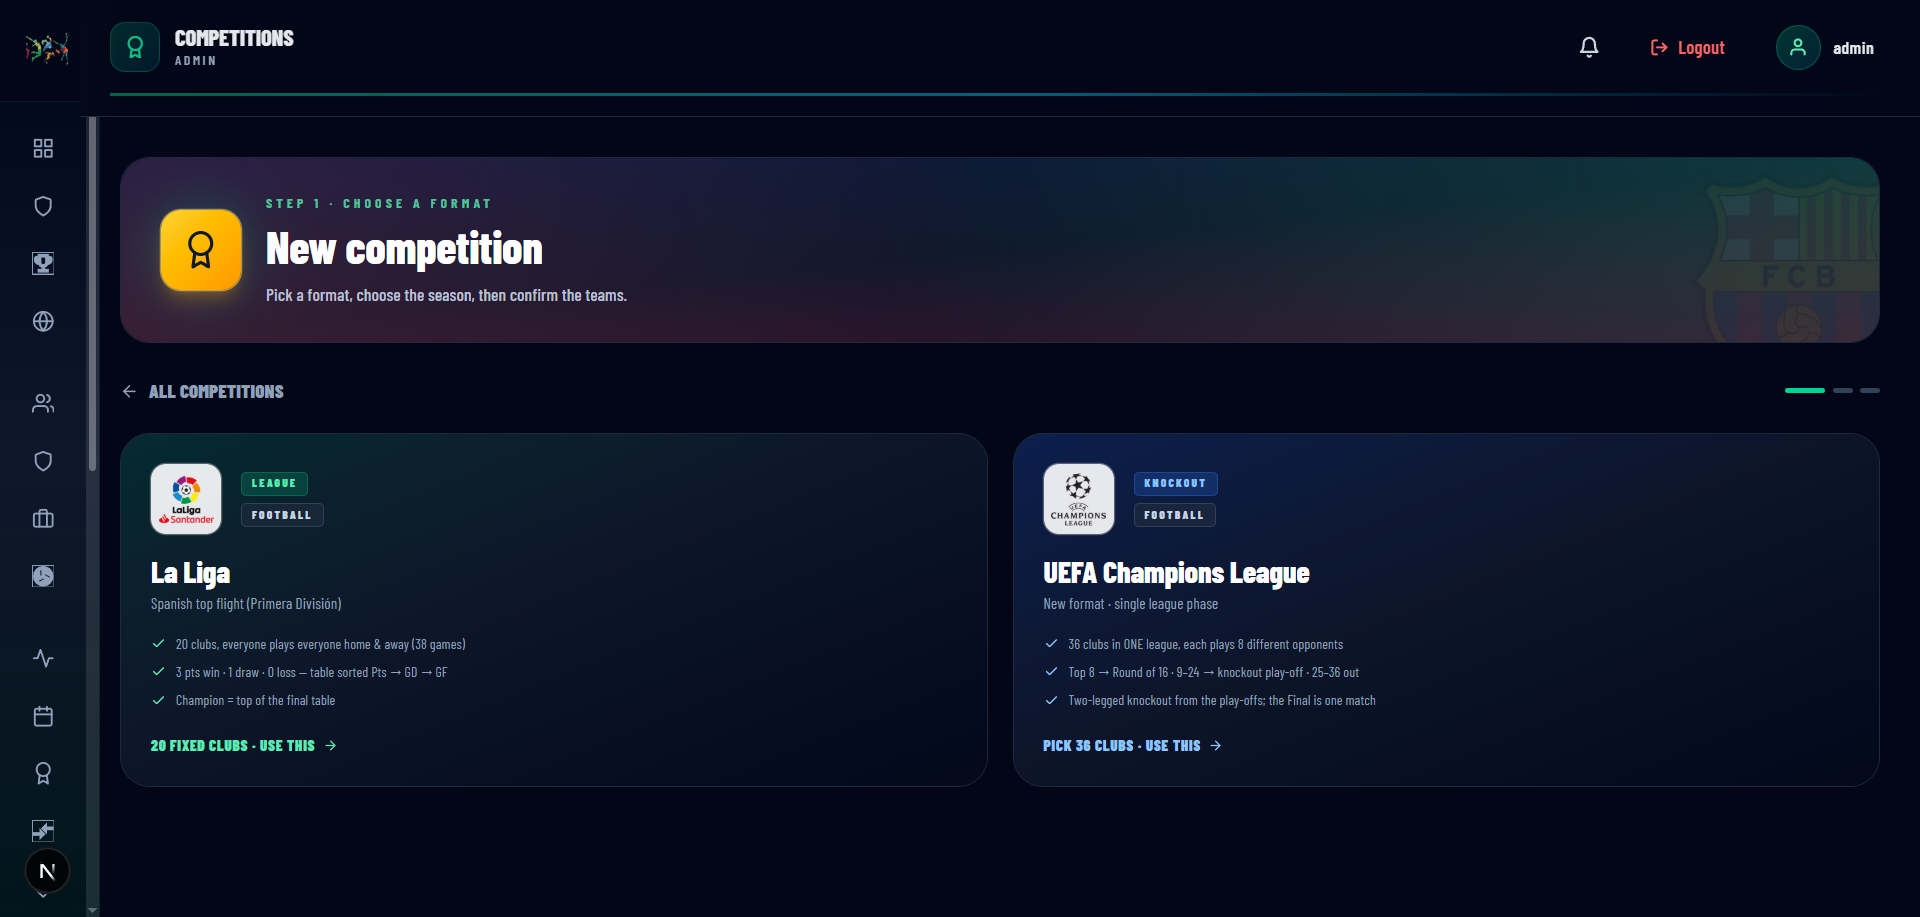
\includegraphics[width=0.9\textwidth]{fig-create-competition.png}
  \caption{The guided competition-creation flow: preset selection, season selection and
  team selection culminate in a generated fixture set persisted by the training-match
  service.}
  \label{fig:create-competition}
\end{figure}

%======================================================================
\section{Head-to-Head Records}
\label{sec:res-h2h}

The Head-to-Head view answers a question that fans and analysts ask constantly but that is
tedious to compute by hand: how has the club fared against a given opponent over time?

\paragraph{User experience.} The page lists every opponent the club has met, and for each one
summarises the all-time record---matches played, won, drawn and lost, together with goals
scored and conceded (Figure~\ref{fig:h2h}). Selecting an opponent expands the individual
fixtures that make up the record, so a headline statistic can be traced back to the matches
that produced it.

\paragraph{Back-end realisation and logic.} The view is computed entirely from the
authoritative \texttt{Match} records held by the training-match service, the same records that
the ingestion pipeline populates and that the live engine writes back to. The front-end groups
the club's matches by opponent and folds each group into a win/draw/loss and goals-for/against
summary using the same scoring conventions as the standings computation, so a head-to-head row
is always consistent with the competition tables. Because it derives from stored results rather
than a separate data source, the record updates automatically as new matches complete---no
manual maintenance of a head-to-head ledger is required.

\begin{figure}[htbp]
  \centering
  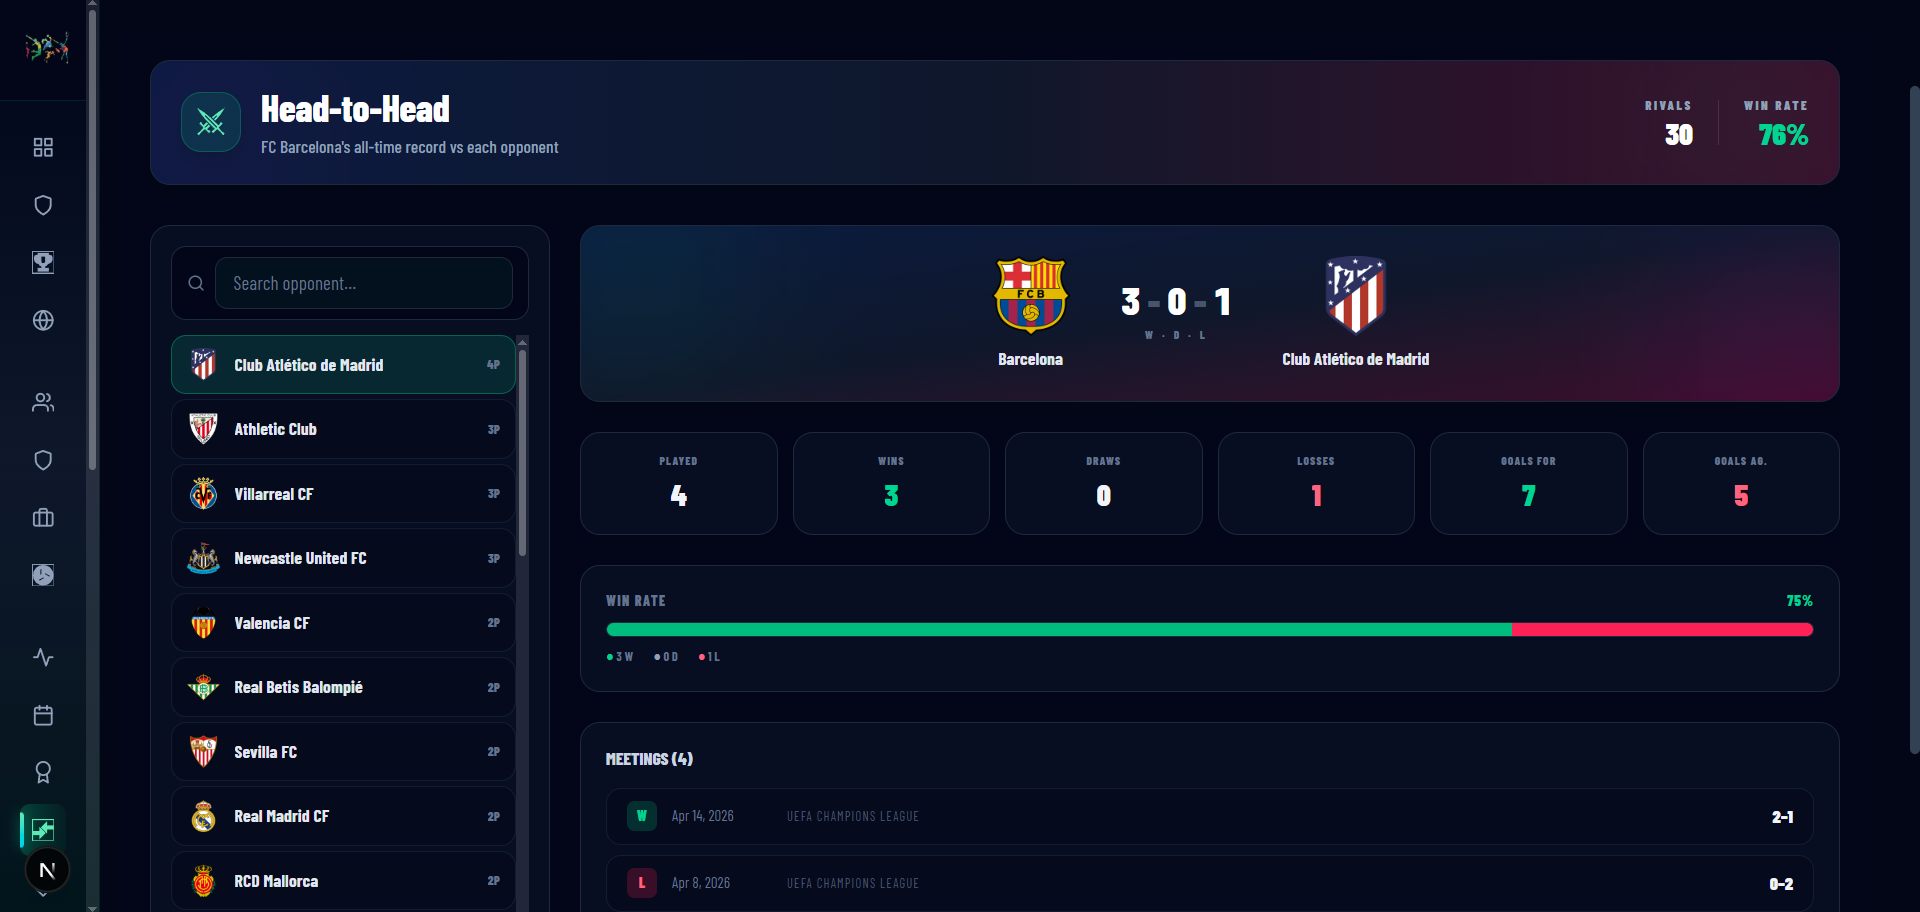
\includegraphics[width=0.95\textwidth]{fig-head-to-head.png}
  \caption{The Head-to-Head view, summarising the club's all-time record against each opponent
  (played, won, drawn, lost and goals) computed from the authoritative match records, with the
  underlying fixtures expandable for any opponent.}
  \label{fig:h2h}
\end{figure}

%======================================================================
\section{World Cup}
\label{sec:res-worldcup}

The World Cup view brings a major international tournament into the platform as live
sporting context, demonstrating that the competition machinery generalises beyond the
club's own two domestic competitions.

\paragraph{User experience.} The page presents the tournament in its real structure: a set
of group tables followed by a knockout bracket that progresses to the final
(Figure~\ref{fig:worldcup}). Group standings and knockout fixtures are shown with the same
visual language as the club's own competitions, so a user moves between the domestic and
international views without re-learning the interface.

\paragraph{Back-end realisation.} As with every external dataset, the front-end never calls
the provider directly. The training-match service exposes read-through endpoints for the
tournament---one that returns the group tables and one that returns the tournament's
matches---so the World Cup competition is available on the provider's free tier and is served
to the browser through the gateway. The group tables are computed and the bracket assembled on
the server side, keeping the browser a pure presentation layer and the API key confined to the
back-end.

\paragraph{Edge cases.} The view is written to render correctly at every phase of the
tournament: before the knockout stage begins it shows only the group tables, and as ties are
decided the bracket fills in progressively, so the page is coherent whether the tournament is
in its group phase, its knockout phase, or complete.

\begin{figure}[htbp]
  \centering
  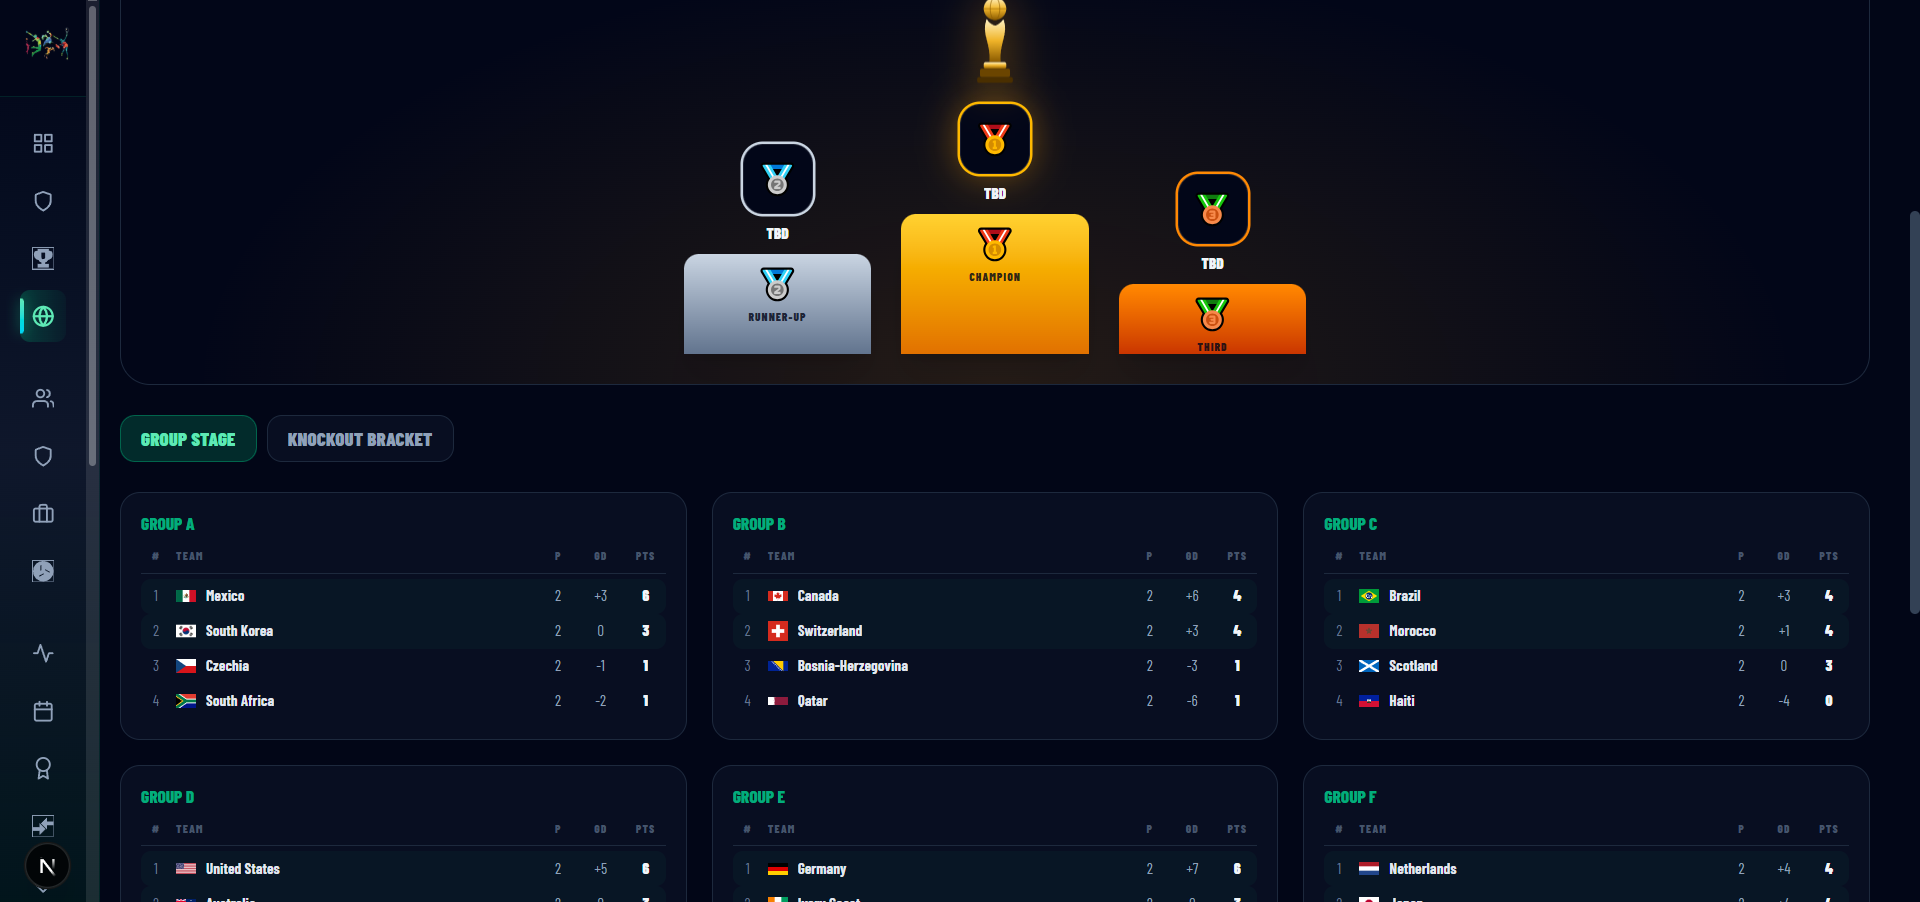
\includegraphics[width=0.95\textwidth]{fig-world-cup.png}
  \caption{The World Cup view, presenting the tournament's group tables and knockout bracket.
  Group standings and the bracket are computed on the server and served to the browser through
  the gateway via read-through endpoints, so the external data provider is never called from
  the client.}
  \label{fig:worldcup}
\end{figure}

%======================================================================
\section{Trophy Room}
\label{sec:res-trophy}

The Trophy Room is the celebratory counterpart to the operational modules: it presents the
club's honours as a curated cabinet, reinforcing the institutional identity that the Club Hub
introduces.

\paragraph{User experience.} The page displays the club's trophies grouped by competition and
era, each rendered as a distinct honour with its competition and the seasons in which it was
won (Figure~\ref{fig:trophy}). The layout is intentionally visual and museum-like, contrasting
with the dense tabular surfaces elsewhere in the product, and gives the platform a sense of
heritage rather than presenting the club as a purely transactional set of records.

\paragraph{Realisation.} The honours are presented as part of the club-identity surface,
complementing the trophy summary shown on the Club Hub with a dedicated, expanded gallery. By
giving the achievements their own room, the platform acknowledges that a club is defined as much
by its history as by its current fixtures, which strengthens the product's claim to be a
faithful digital home for the institution rather than a back-office tool.

\begin{figure}[htbp]
  \centering
  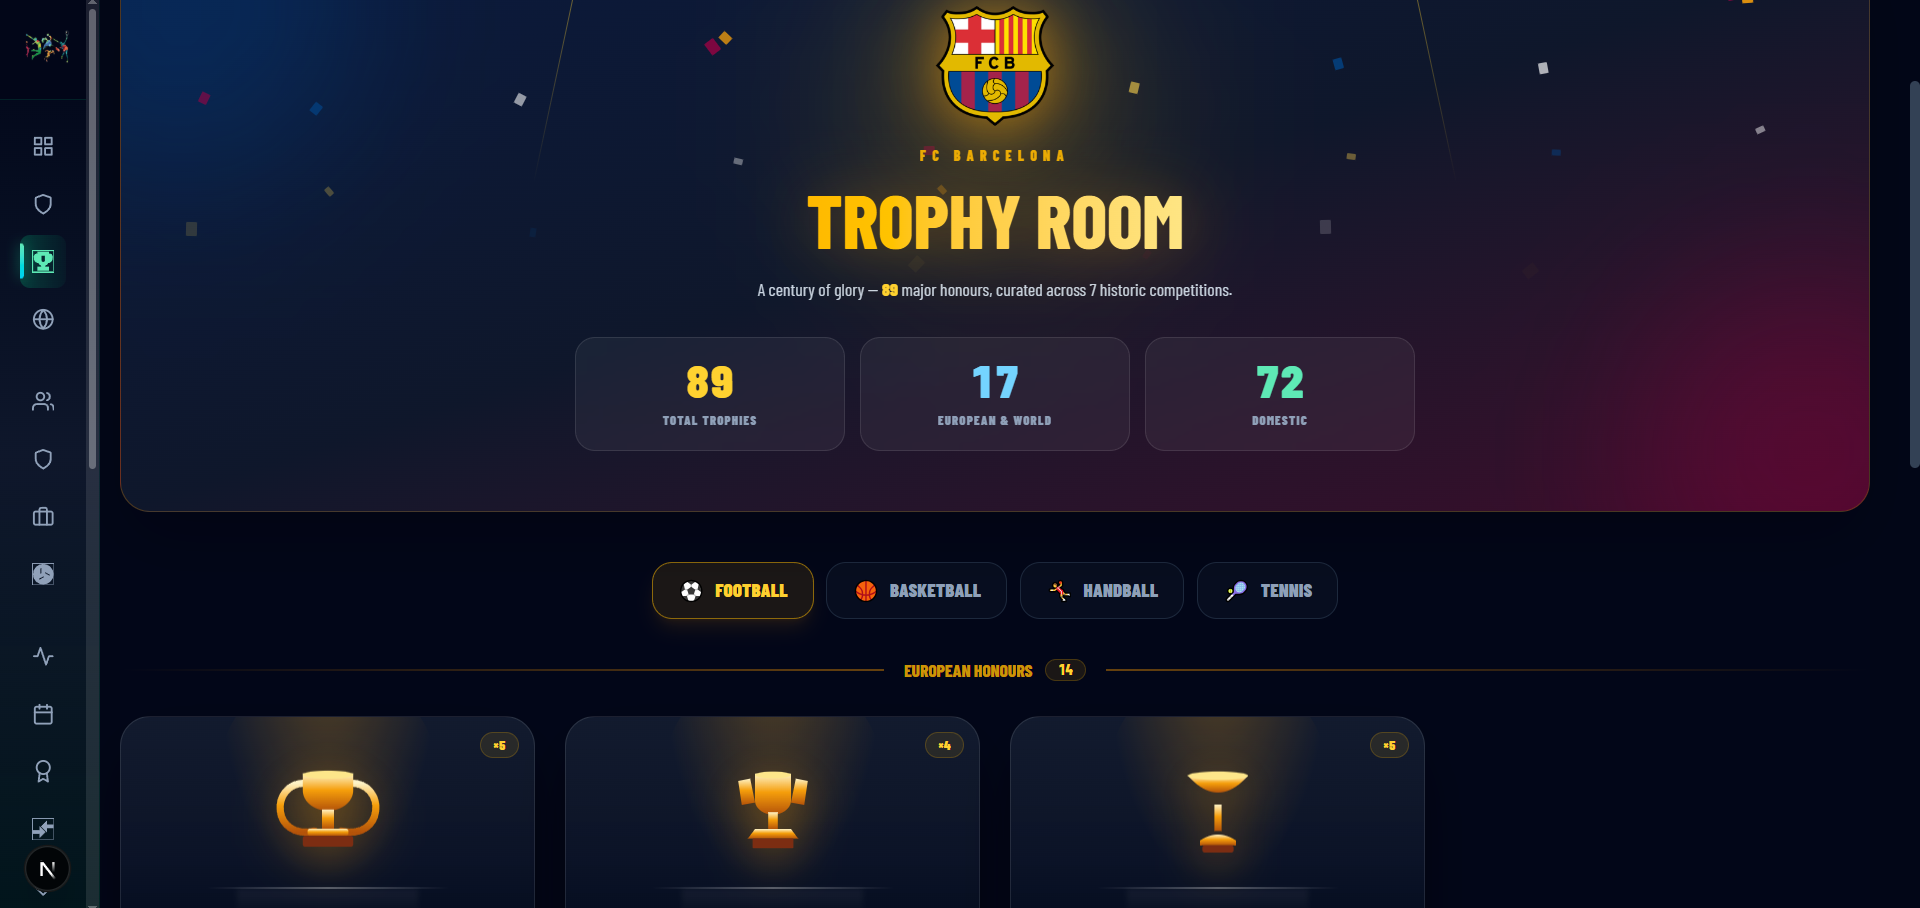
\includegraphics[width=0.9\textwidth]{fig-trophy-room.png}
  \caption{The Trophy Room, presenting the club's honours as a curated cabinet grouped by
  competition and era, complementing the trophy summary on the Club Hub.}
  \label{fig:trophy}
\end{figure}

%======================================================================
\section{Match Hub}
\label{sec:res-matches}

The Match Hub is the operational list of the club's own matches---the matches it schedules,
plays and reviews, as distinct from the external fixtures surfaced in the competition views.

\paragraph{User experience.} It comprises a \emph{Schedule a match} action, four status filters
(Scheduled, Live, Completed and a catch-all) and a team filter, with each match rendered as a
card showing the opponent's name and crest, the kickoff time, and---for upcoming matches---a
live countdown that flips the card to a \texttt{LIVE} state automatically when kickoff arrives
(Figure~\ref{fig:matches}). The countdown is computed entirely client-side from the stored
kickoff timestamp, so a card transitions to live without any server round-trip and without the
user refreshing the page.

\paragraph{Self-cleaning behaviour.} The Hub also performs housekeeping on load to keep the list
trustworthy without manual intervention. Matches that were scheduled or marked live but have
passed kickoff by more than ninety minutes with no recorded events are treated as abandoned and
removed---these are typically test or mistakenly created matches that were never played. Matches
that carry real events but were never formally ended are finalised to a completed state. To make
finished matches self-consistent, goal events are backfilled so that each completed match's
recorded scorers reconcile with its final score, drawing the scorers from the saved starting XI.
The net effect is that the Match Hub always presents a clean, internally consistent record, and a
stray or interrupted match cannot accumulate as noise.

\begin{figure}[htbp]
  \centering
  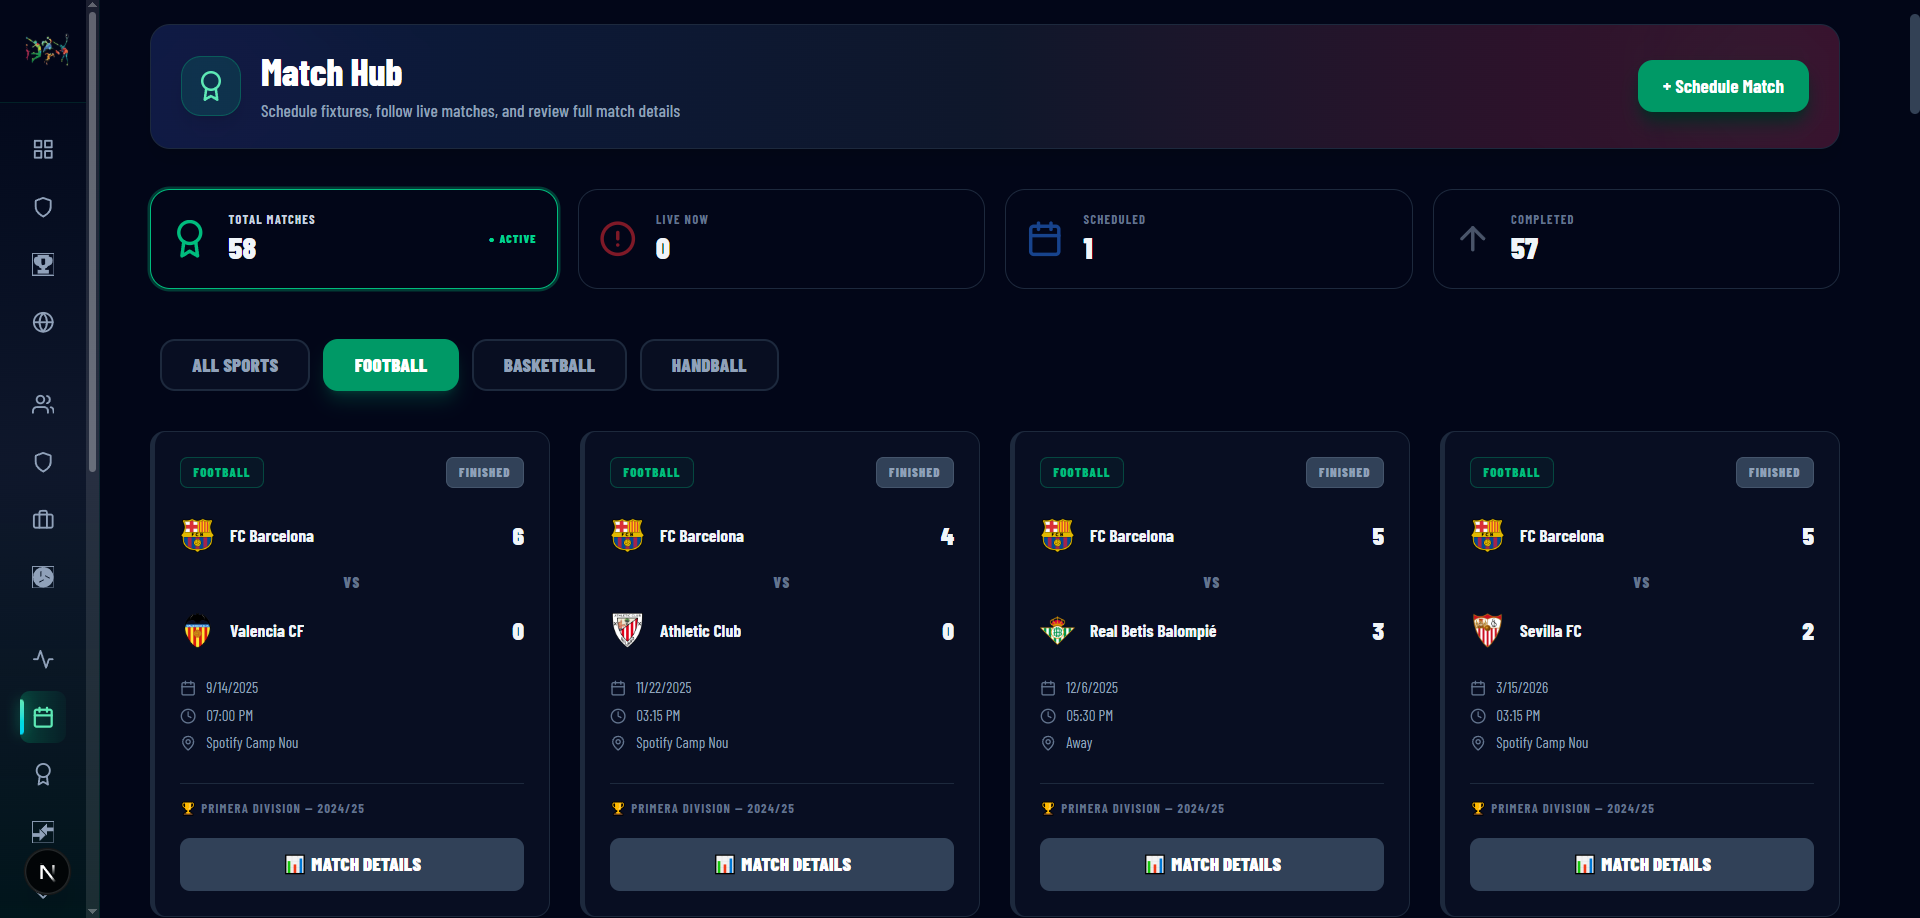
\includegraphics[width=0.95\textwidth]{fig-matches.png}
  \caption{The Match Hub, listing the club's matches with status and team filters and a
  schedule action. Upcoming cards display a live countdown and transition to a LIVE state
  at kickoff.}
  \label{fig:matches}
\end{figure}

\subsection{Scheduling a Match}
\label{sec:res-match-schedule}

Scheduling distinguishes between a \emph{Friendly} and an \emph{Official} match
(Figure~\ref{fig:match-schedule}). A Friendly allows a free choice of opponent, whereas an
Official match is bound to a real, still-running competition and offers only that competition's
unplayed fixtures, carrying the fixture's identity forward so that the eventual result can be
written back to the source. This binding is what closes the loop between the live engine and the
competition record: an official match is not an island, but an instance of a specific
competition fixture.

\paragraph{Kickoff validation.} The kickoff time is validated to lie at least five minutes in the
future. The validation is a pure function of the chosen timestamp and the current time: it rejects
an empty value, an unparseable value, a value in the past, and a value less than five minutes
ahead, returning a specific user-facing message for each case. The picker itself advertises a
minimum selectable value of ``now plus five minutes'', nudging the user toward a valid choice
before they even submit. A subtle but important detail is that the kickoff is stored as a naive
local wall-clock string rather than being passed through a timezone conversion: an earlier defect
in which times were shifted by the local UTC offset (making matches appear several hours early and
spuriously live) was fixed by normalising the picker value to the back-end's naive
\texttt{LocalDateTime} format without any UTC arithmetic.

\paragraph{Lineup is mandatory.} Critically, a match is never persisted on its own: a lineup is
required. The scheduling form stages its payload and hands off to the lineup builder, and only when
a formation and starting eleven are confirmed does the system create the match, its formation and
its lineup together in one coherent operation. This guarantees a key invariant exploited everywhere
downstream---every match in the system, the moment it exists, already has a reconstructable starting
XI.

\begin{figure}[htbp]
  \centering
  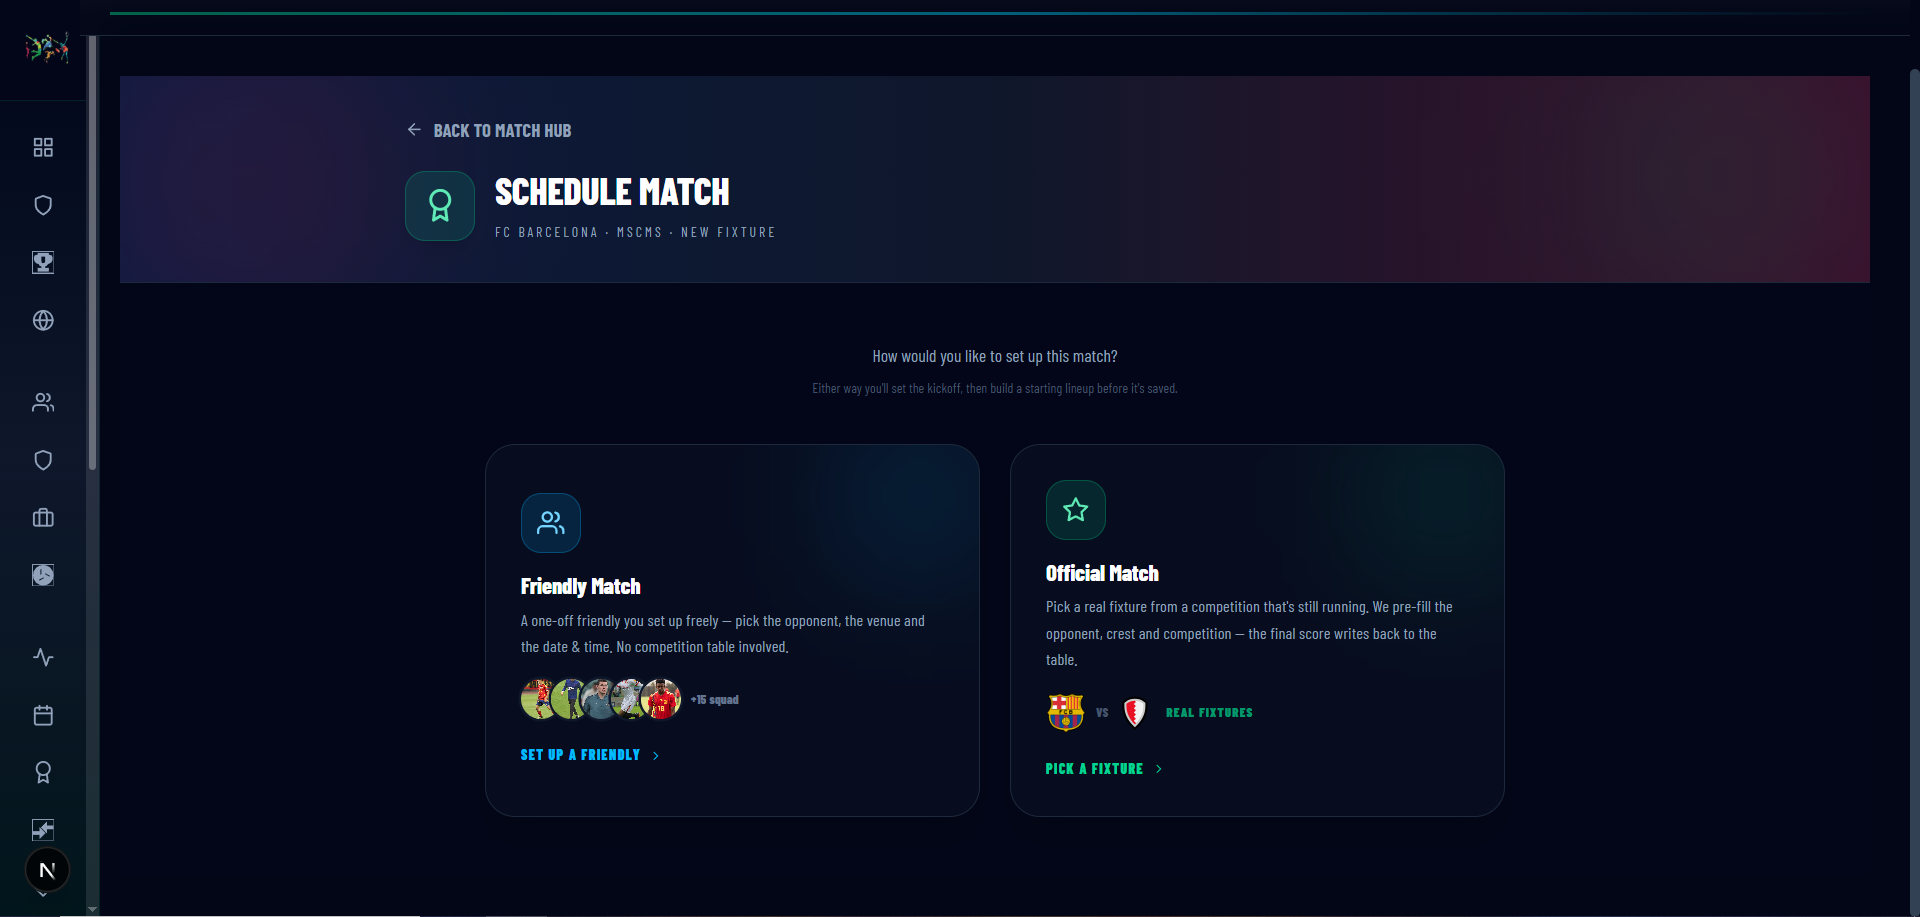
\includegraphics[width=0.9\textwidth]{fig-match-schedule.png}
  \caption{Scheduling a match. The Friendly/Official chooser, opponent or fixture
  selection and a future-dated kickoff feed a draft that is only persisted once a lineup
  has been confirmed.}
  \label{fig:match-schedule}
\end{figure}

\subsection{The Lineup Builder}
\label{sec:res-lineup}

The lineup builder is a formation-first, interactive pitch (Figure~\ref{fig:lineup}).

\paragraph{User experience.} The user begins by selecting a formation appropriate to the sport,
after which players are placed and rearranged on the pitch by drag-and-drop, with each position
rendered as a card bearing the player's photograph. A single-card drag ghost gives the drag
operation a clean, unambiguous visual, and players can be swapped between positions or between the
pitch and the bench. The starting eleven and the bench are assembled here.

\paragraph{Back-end realisation and data model.} The builder is backed by two entities in the
training-match service. A \texttt{MatchFormation} captures the chosen shape and a compact
\texttt{formationDetails} description, while \texttt{MatchLineup} records the per-player placements.
These are exposed through \texttt{/match-formations} and \texttt{/match-lineups} endpoints and are
saved atomically with the match. A practical constraint worth recording is that the
\texttt{formationDetails} column is a bounded \texttt{VARCHAR(255)}, so the encoding is kept compact
to avoid an over-length write being rejected---a small but real example of the data model shaping
the client encoding.

\paragraph{Why this matters.} Because the lineup is captured at creation time and locked thereafter,
every completed match in the system carries a genuine, reconstructable starting XI rather than a
placeholder. This is precisely what makes the in-match event and substitution logic meaningful: a
substitution refers to real players who were really on the pitch, an in-match injury flags a real
squad member, and the match-details page can rebuild the exact eleven that started. The entire fifty-odd
finished football matches in the seed data were backfilled with real starting elevens for the same
reason, so that the historical record is as self-consistent as a freshly scheduled match.

\begin{figure}[htbp]
  \centering
  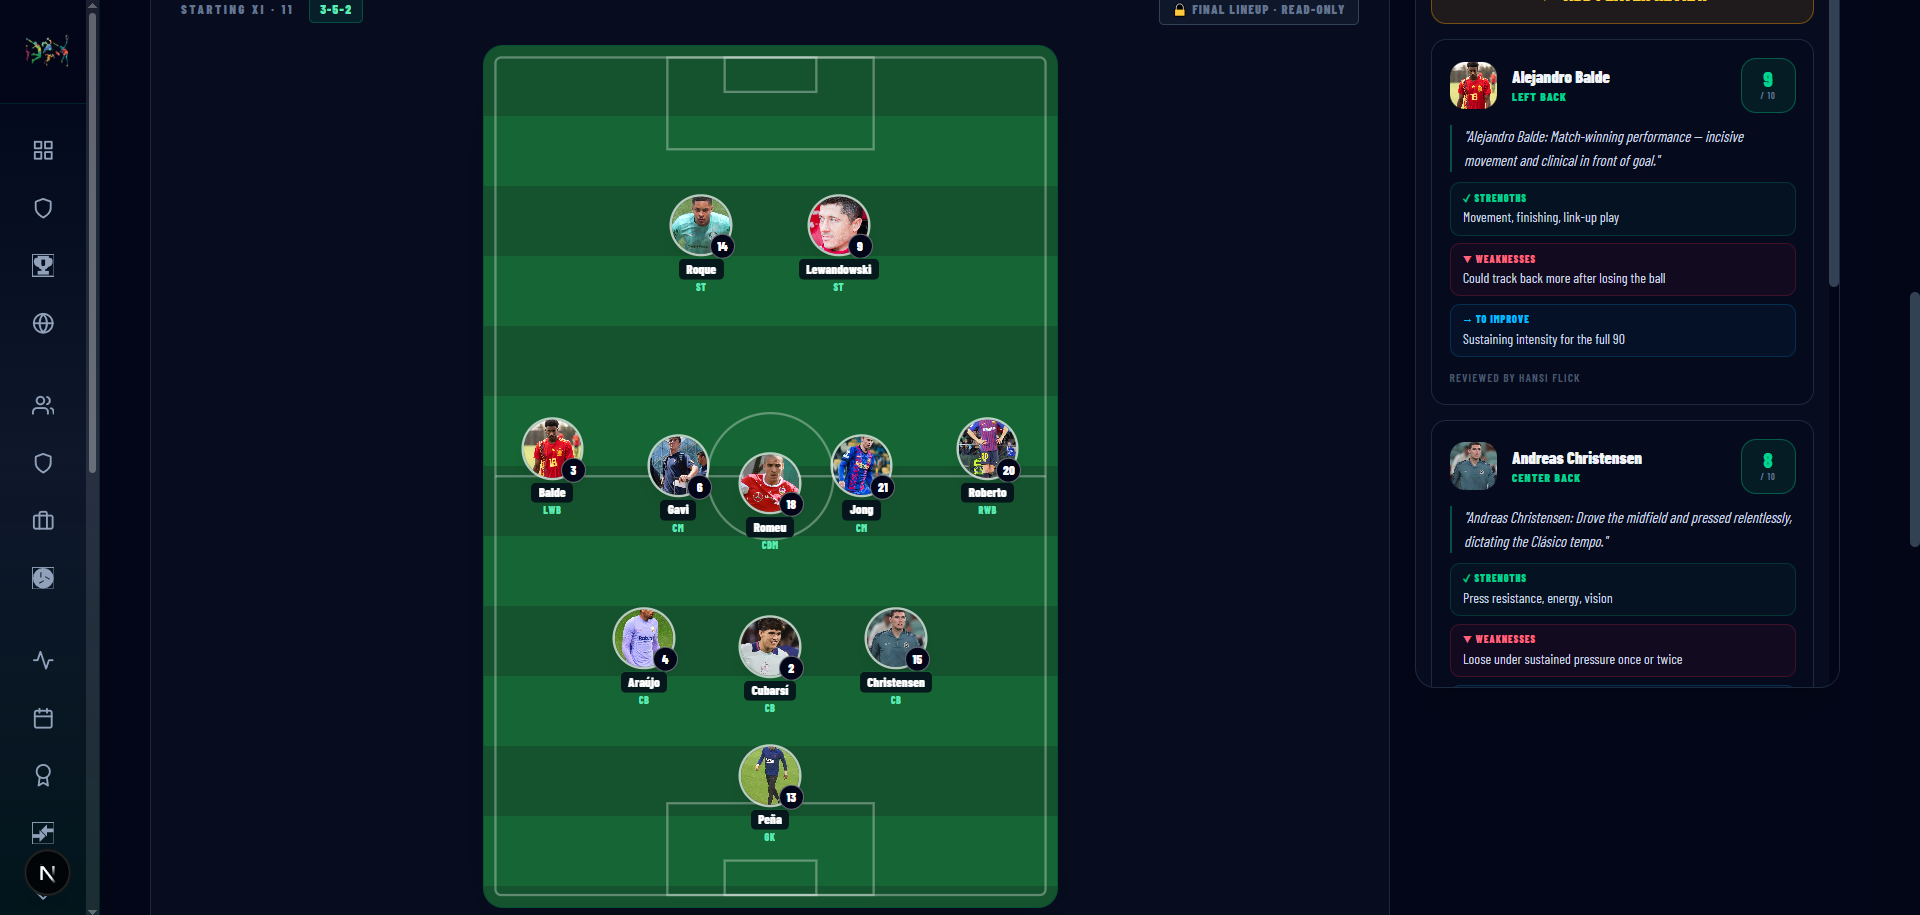
\includegraphics[width=0.95\textwidth]{fig-lineup.png}
  \caption{The formation-first lineup builder. Players are positioned on the pitch by
  drag-and-drop, and the resulting formation and starting XI are persisted atomically with
  the match.}
  \label{fig:lineup}
\end{figure}

%======================================================================
\section{The Live-Match Engine}
\label{sec:res-live}

The live-match engine is the most behaviourally rich component of the platform, and the one in
which the front-end and back-end cooperate most tightly. It transforms a static fixture into a
real-time, broadcast-style operational surface (Figure~\ref{fig:live-match}).

\subsection{Gating and Auto Go-Live}
Control of the engine is gated until kickoff is reached or the match is already live, so a match
cannot be operated before it is due to begin. The transition itself is automatic: pure timestamp
helpers compute, from the stored kickoff and the current time, whether kickoff has arrived, the
running match minute, and the phase the minute implies. When the kickoff moment passes, the match
goes live on its own---the user never manually flips it---and the elapsed minute begins advancing.
Because these computations are pure functions of two timestamps, the common case of simply watching
the clock advance requires no server round-trip, which keeps the live view responsive.

\subsection{The Phase Machine}
The engine drives a broadcast-style \emph{phase machine}. Each phase is described by a small record
giving its label, the base minute at which its clock starts, its regulation length, whether it is a
playing phase with a running clock, and the phase that follows it. The regulation sequence is
\texttt{FIRST\_HALF}~(45') $\rightarrow$ \texttt{HALF\_TIME} $\rightarrow$
\texttt{SECOND\_HALF}~(45') $\rightarrow$ \texttt{FULL\_TIME}. For a true knockout tie that remains
level at full time, the machine extends into \texttt{EXTRA\_FIRST}~(15') $\rightarrow$
\texttt{EXTRA\_HALFTIME} $\rightarrow$ \texttt{EXTRA\_SECOND}~(15') and, if still level, a
\texttt{PENALTIES} shootout, which is a non-timed state owned explicitly by the user interface. For a
points fixture---including a Champions League league-phase match---a draw is a legitimate result and
the engine stops at full time.

\paragraph{Resolving knockout from points authoritatively.} The knockout-versus-points decision is
the linchpin of the whole machine, and it is resolved authoritatively rather than guessed. A set of
match types (league, friendly, group and the various league-stage labels) are treated as
points fixtures for which a draw is valid; but when a match originates from a real competition fixture,
the resolved round of that fixture is checked \emph{first} and overrides the loose type. The effect is
that a match stored loosely as a tournament match is still correctly treated as a draw-permitting league
fixture when its round indicates the league phase, and a genuine knockout tie correctly extends into
extra time and penalties. Threading the decision through the originating fixture's round is what keeps
the engine consistent with the competition format described in
Section~\ref{sec:res-cl-bracket}.

\subsection{The Clock, Stoppage Time and Phase-Bounded Minutes}
Each playing phase exposes an administrator-set stoppage time, allowing the clock to read ``45+3''' or
``90+5''' during added time. The clock is carefully bounded so that it can never run away into nonsense.
The displayed minute is hard-capped at the phase's regulation length, and the added portion shown is the
\emph{admin-set} stoppage only, never the raw elapsed overflow. Consequently a half left running for an
extended period freezes at, for example, ``45+3''' (or simply ``45''' when no stoppage was set) rather
than inflating into an absurd minute---a concrete defect (an observed ``45+132''') that was fixed by this
capping rule. It is always the user who advances the phase; the clock follows, it does not lead.

Event entry is likewise phase-bounded. The recordable-minute range is computed per phase: the first half
accepts minutes one to forty-five plus any stoppage, the second half forty-six to ninety plus stoppage,
and each extra-time period its fixed fifteen-minute window. Non-playing phases (the half-time and full-time
intervals, the extra-time interval and the penalty shootout) carry no recordable minute. This prevents a
nonsensical entry such as a first-half goal recorded at minute eighty, and it means that when state is
reconstructed on reload, a stored event minute maps unambiguously back to the phase in which it occurred.

\subsection{Events, Scoring and Substitutions}
Events are entered against the live clock and persist immediately through the match-events API. A
\texttt{MatchEvent} entity records the event type, the minute, the acting player's \texttt{keycloakId} and
a free-text description; the event-type enumeration is broad and sport-aware, covering goals, assists,
penalties scored and missed, own goals, yellow and red cards, corners, free kicks, offsides and VAR reviews
for football, as well as the equivalent events for basketball, handball, tennis, volleyball and swimming.
Scoring events increment the appropriate side's tally, and the running score is written back to the match as
play proceeds.

Substitutions have a dedicated control that records the outgoing and incoming players and the minute. Because
the underlying \texttt{MatchEvent} carries a single player reference, a substitution encodes both players---their
numeric identifiers, their \texttt{keycloakId}s and their names---in a parseable tag inside the event description,
which lets the timeline render both faces and lets the post-match review form learn which substitutes actually
came on. Substitutions are limited per sport: football permits the modern maximum of five, while free-interchange
roster sports such as basketball and handball are effectively unlimited. The engine tracks which players have left
the pitch, which substitutes have entered, and how many of the allowance has been consumed, and it rebuilds this
on-pitch set on reload from the stored events so that the live state survives a page refresh.

\subsection{The In-Match Injury Bridge}
An in-match \texttt{INJURY} event does double duty and is the clearest demonstration of genuine cross-service
integration. It is recorded as an ordinary match event \emph{and} simultaneously creates a real injury record in
the medical-fitness service: the engine posts a new injury (in the \texttt{REPORTED} status, linked to the player,
with a chosen injury type and severity) and then flips the affected player's status to \texttt{INJURED} through the
player-management API. The consequences ripple outward without any further action: the injured player is forced off
the pitch and, because an injury substitution is exempt from the normal sub-count, the replacement is always
permitted even past the five-substitution limit; the player becomes unselectable in future lineups, match selection
and training; and the incident appears in the Medical module's Treatment Room ready for the staged clinical journey
described in Section~\ref{sec:res-medical}. A single click in the live engine thus drives three services at once.

\subsection{Alerts and Result Write-Back}
Recording a goal raises a real, persisted alert so that interested roles are notified as the match unfolds, and
ending the match emits a result-available alert and writes the final score back to the source competition fixture.
The alert posting is best-effort and resilient: the engine attempts a goal-scored alert type and, because the
back-end alert enumeration must be respected, falls back to a valid match-scoped type if necessary so that a real
alert is always created and the call never throws. Ending an official match writes the final score to its originating
fixture, which in turn moves the competition standings (Section~\ref{sec:res-laliga}) and, where relevant, unlocks or
advances the knockout bracket. This closes the loop between live operations, the notification fabric and the
competition record, so that operating a live match is not a self-contained activity but one that updates the whole
platform.

\begin{figure}[htbp]
  \centering
  \IfFileExists{screenshots/fig-live-match.png}{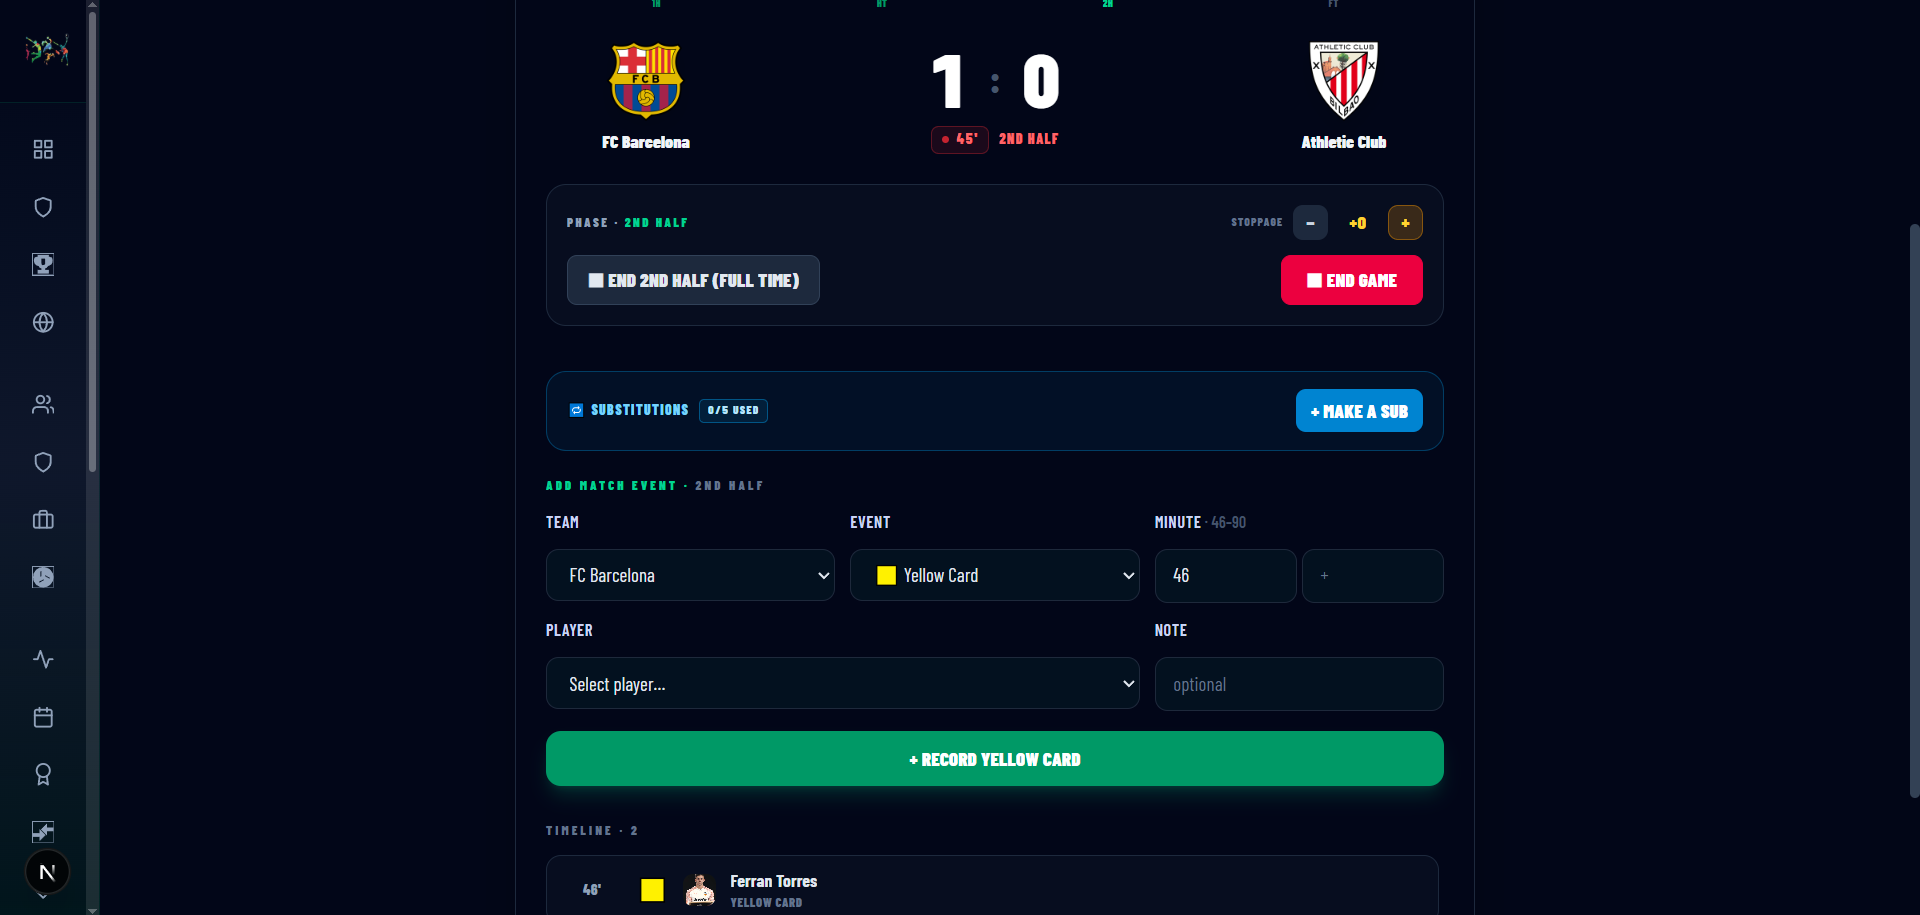
\includegraphics[width=0.95\textwidth]{fig-live-match.png}}{\fbox{\parbox[c][5cm][c]{0.9\textwidth}{\centering\itshape Live-match control panel --- screenshot to be inserted (\texttt{fig-live-match.png}).}}}
  \caption{The live-match engine. The broadcast-style phase machine, stoppage-time
  control, event entry, per-sport substitutions and in-match injury recording drive the
  match in real time and persist every action to the back-end.}
  \label{fig:live-match}
\end{figure}

\subsection{Match Details: Events, Statistics and Reviews}
\label{sec:res-match-details}

Once a match is complete its detail page becomes a read-only record of what occurred
(Figure~\ref{fig:match-details}). It reconstructs the saved starting XI on a pitch board, presents a
chronological events timeline, a statistics panel, and a reviews wall on which coaching staff record
post-match player assessments. The reviews wall reads the substitution events to learn which substitutes
came on, so an assessment can be recorded for a player who only featured for the closing minutes, not merely
for the eleven who started. Because every finished match carries a real lineup and a backfilled set of goal
events consistent with its score, the detail page presents a faithful, self-consistent account of the match
rather than a synthetic summary, and a finished match is rendered read-only in keeping with the platform-wide
treatment of completed records.

\begin{figure}[htbp]
  \centering
  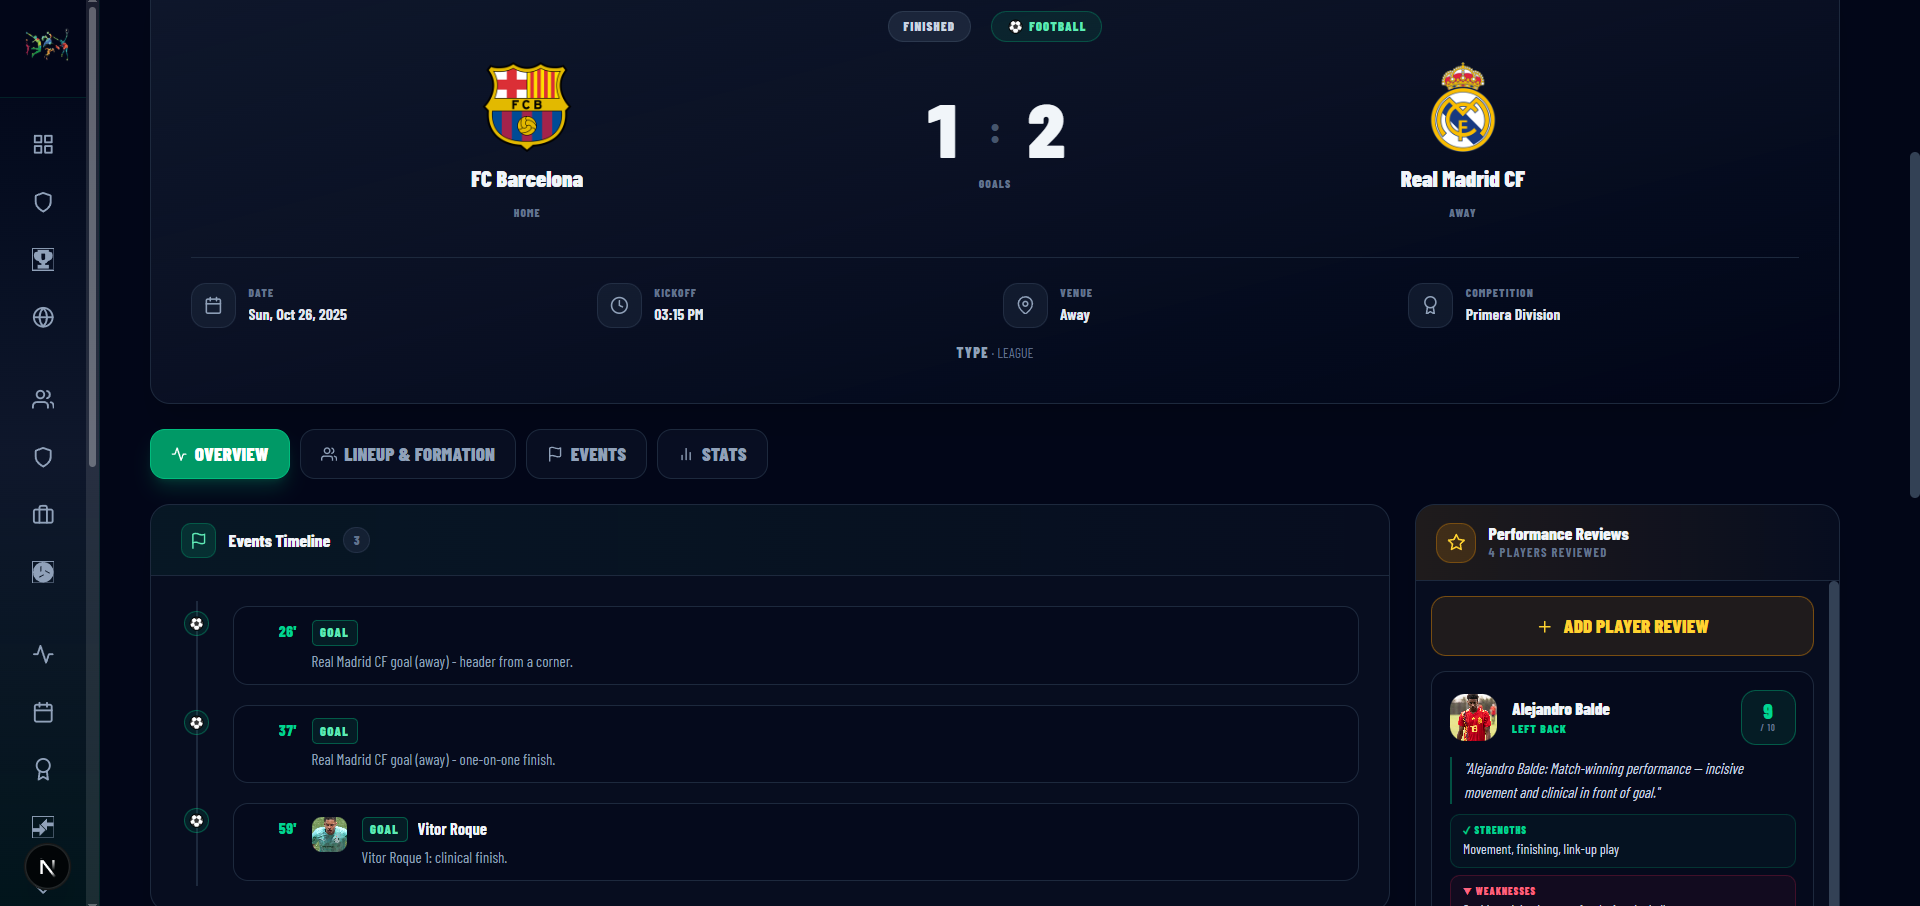
\includegraphics[width=0.95\textwidth]{fig-match-details.png}
  \caption{The match details page, presenting the reconstructed starting XI, the events
  timeline, match statistics and the post-match player-review wall for a completed match.}
  \label{fig:match-details}
\end{figure}

%======================================================================
\section{Medical and Fitness}
\label{sec:res-medical}

The medical module, served by the medical-fitness service (port~8086), manages the full clinical lifecycle
of a player's injury. It is one of the modules that most clearly transcends simple record-keeping, encoding a
genuine clinical workflow rather than a flat table of incidents.

\paragraph{The Treatment Room.} The module's centrepiece is the \emph{Treatment Room}, which divides the squad
into \emph{Currently Injured} and \emph{Recovered} cohorts (Figure~\ref{fig:medical-room}). A player is
considered injured---and is automatically withdrawn from upcoming matches, lineups and training---from the moment
an injury is logged until a passing fitness test clears them back to availability. This withdrawal is achieved
not by editing every dependent module but by the player's single \texttt{status} field, which every other module
already respects, so the squad's operational status stays consistent across the match and training modules without
any manual reconciliation.

\paragraph{Back-end realisation and data model.} An \texttt{Injury} entity records the affected player, the body
part, the injury type and severity, the report metadata, and---most importantly---a \texttt{status} drawn from a
small enumeration: \texttt{REPORTED}, \texttt{DIAGNOSED}, \texttt{TREATING}, \texttt{RECOVERING},
\texttt{RECOVERED} and \texttt{CHRONIC}. The injury aggregates its associated clinical sub-records: diagnoses,
treatments and rehabilitation entries, with recovery programmes and fitness tests recorded as the journey
advances. The injury exposes a conventional REST surface for creation and retrieval, and it is this entity that the
live-match engine targets when an in-match injury occurs.

\begin{figure}[htbp]
  \centering
  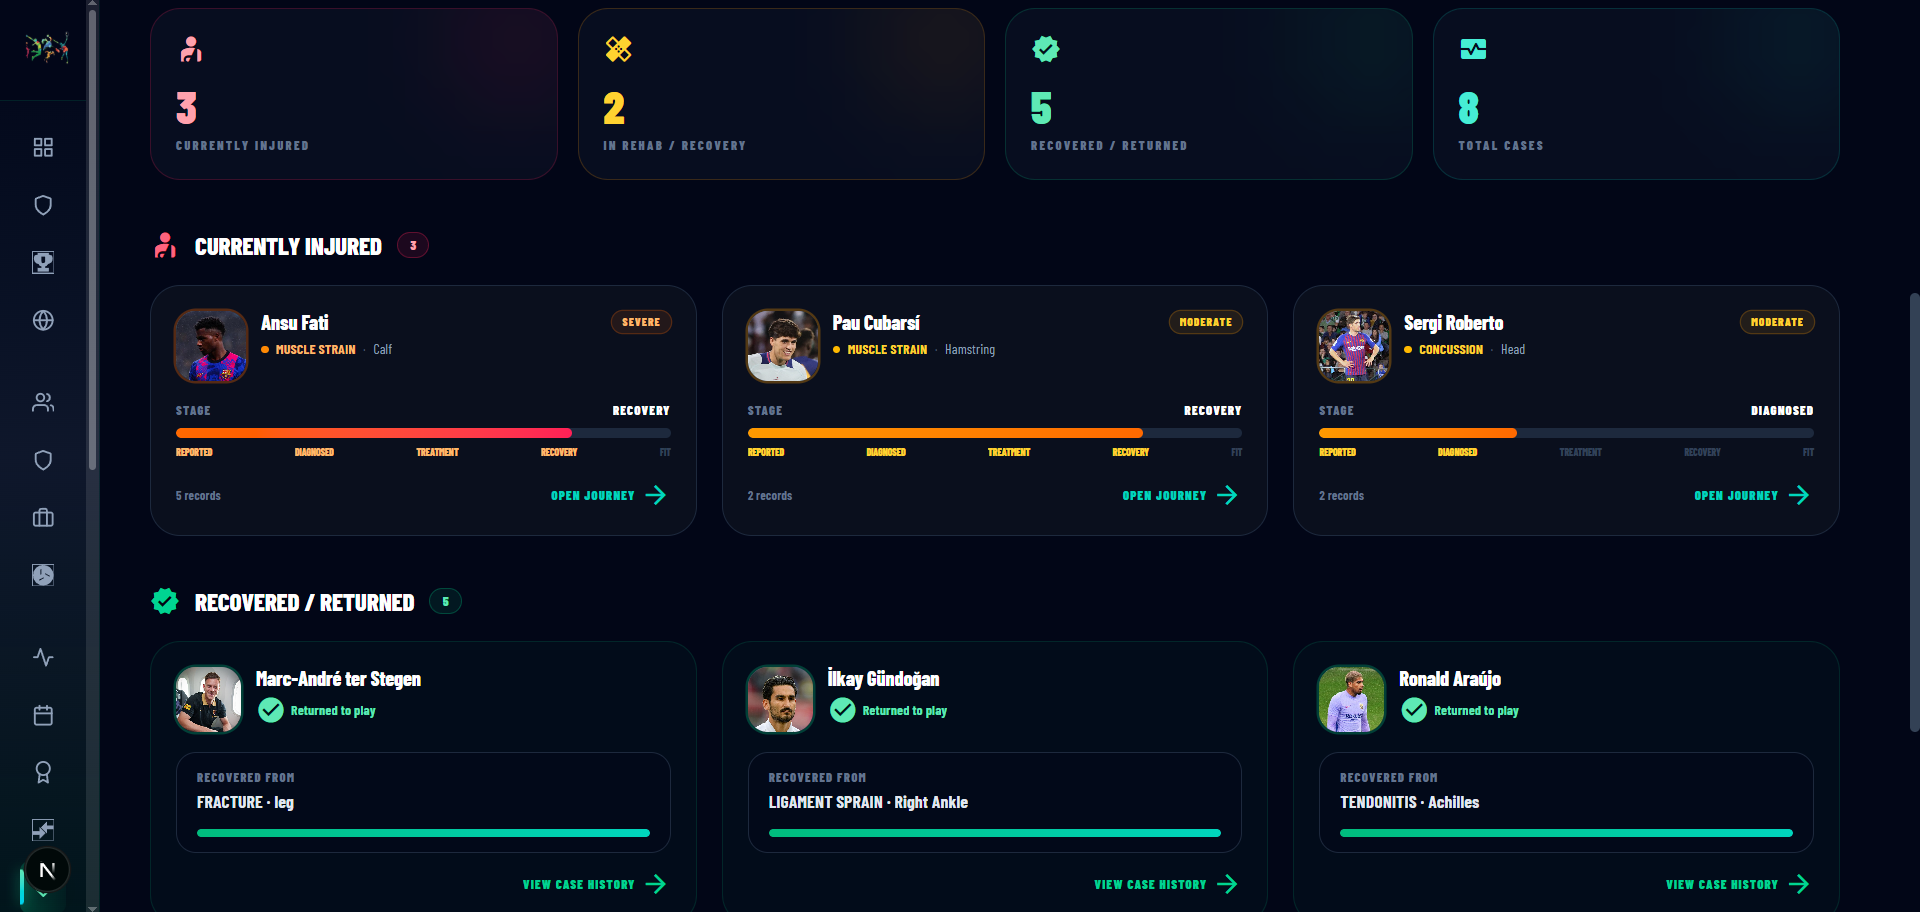
\includegraphics[width=0.95\textwidth]{fig-medical-room.png}
  \caption{The Medical Treatment Room, separating currently injured players from those who
  have recovered. Logging an injury automatically withdraws the player from matches,
  lineups and training until a passing fitness test restores availability.}
  \label{fig:medical-room}
\end{figure}

\subsection{The Injury Journey}
\label{sec:res-medical-journey}

Each injured player has a staged recovery journey rendered as a stepper:
Injury~$\rightarrow$~Diagnosis~$\rightarrow$~Treatment~$\rightarrow$~Rehabilitation~$\rightarrow$~Recovery~$\rightarrow$~Fitness~Test~$\rightarrow$~Recovered
(Figure~\ref{fig:medical-journey}).

\paragraph{Status as the single source of truth.} The injury's own status is the single source of truth for how far
the player has progressed, and this is the design decision that makes the workflow robust. Rather than inferring the
current stage from whichever sub-records happen to exist---an approach that breaks down the moment a stray document
is left over from a previous episode---the stepper reads the injury's status directly and maps it onto the stage. As
the player progresses, the status advances through the enumeration: an initial report is \texttt{REPORTED}, a recorded
diagnosis moves it to \texttt{DIAGNOSED}, treatment to \texttt{TREATING}, and so on through \texttt{RECOVERING} to
\texttt{RECOVERED}. Because the stage is read from one authoritative field, the stepper always reflects the true
clinical state and is immune to leftover sub-records, which was a concrete source of confusion before the status-driven
design was adopted.

\paragraph{Ordered progression.} Advancing a stage records a new clinical document---a diagnosis, a treatment, a
rehabilitation plan, a recovery programme or a fitness-test result---and the journey enforces the correct ordering. It
guarantees, for example, that a rehabilitation record exists before a recovery programme can be created, so the clinical
history reads as a coherent sequence rather than an arbitrary set of documents. Only a \emph{passing} fitness test
completes the journey: it moves the injury to recovered and returns the player to the available pool, at which point the
player reappears in lineup pickers, match selection and training. A failing fitness test does not clear the player,
keeping a not-yet-fit player correctly withheld from selection.

\begin{figure}[htbp]
  \centering
  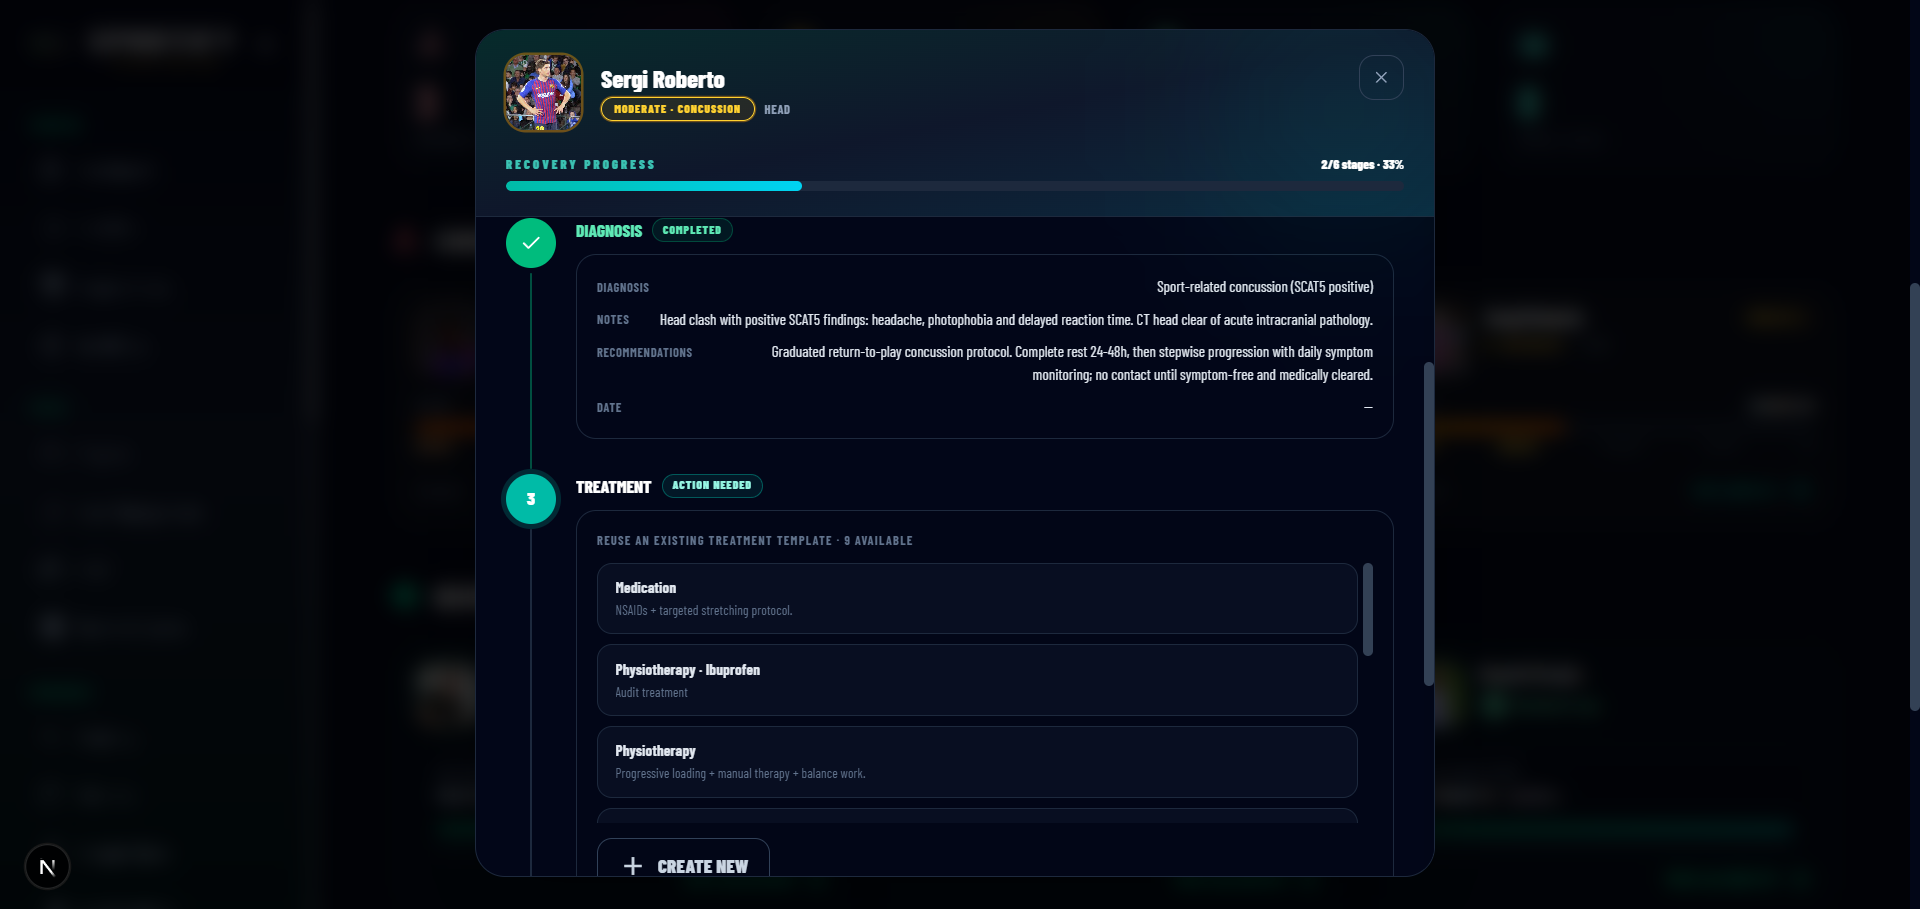
\includegraphics[width=0.95\textwidth]{fig-medical-journey.png}
  \caption{The per-player injury journey stepper, progressing from the initial injury
  through diagnosis, treatment, rehabilitation, recovery and a fitness test to full
  recovery. The injury's status is the single source of truth for the current stage.}
  \label{fig:medical-journey}
\end{figure}

\subsection{General Medical Catalogs}
\label{sec:res-medical-catalog}

Alongside the per-player journey, the module exposes general catalogs for each clinical category---Injuries, Diagnoses,
Treatments, Rehabilitation, Recovery and Fitness Tests (Figure~\ref{fig:medical-catalog}). These provide reusable,
browsable records and serve as templates that the journey's stage pickers can draw upon.

\paragraph{Copy, not link.} A subtle but deliberate design choice governs how a catalog entry is used: selecting one
pre-fills the relevant stage form, but its content is then \emph{copied} into a fresh record for the current player rather
than re-linked to the shared template. This preserves a clean, independent per-injury history---editing a player's
treatment record cannot retroactively mutate the shared catalog, and the catalog cannot change a player's recorded
history---while still saving the clinician the effort of re-entering common information. The result combines the
convenience of templates with the integrity of immutable per-episode records.

\begin{figure}[htbp]
  \centering
  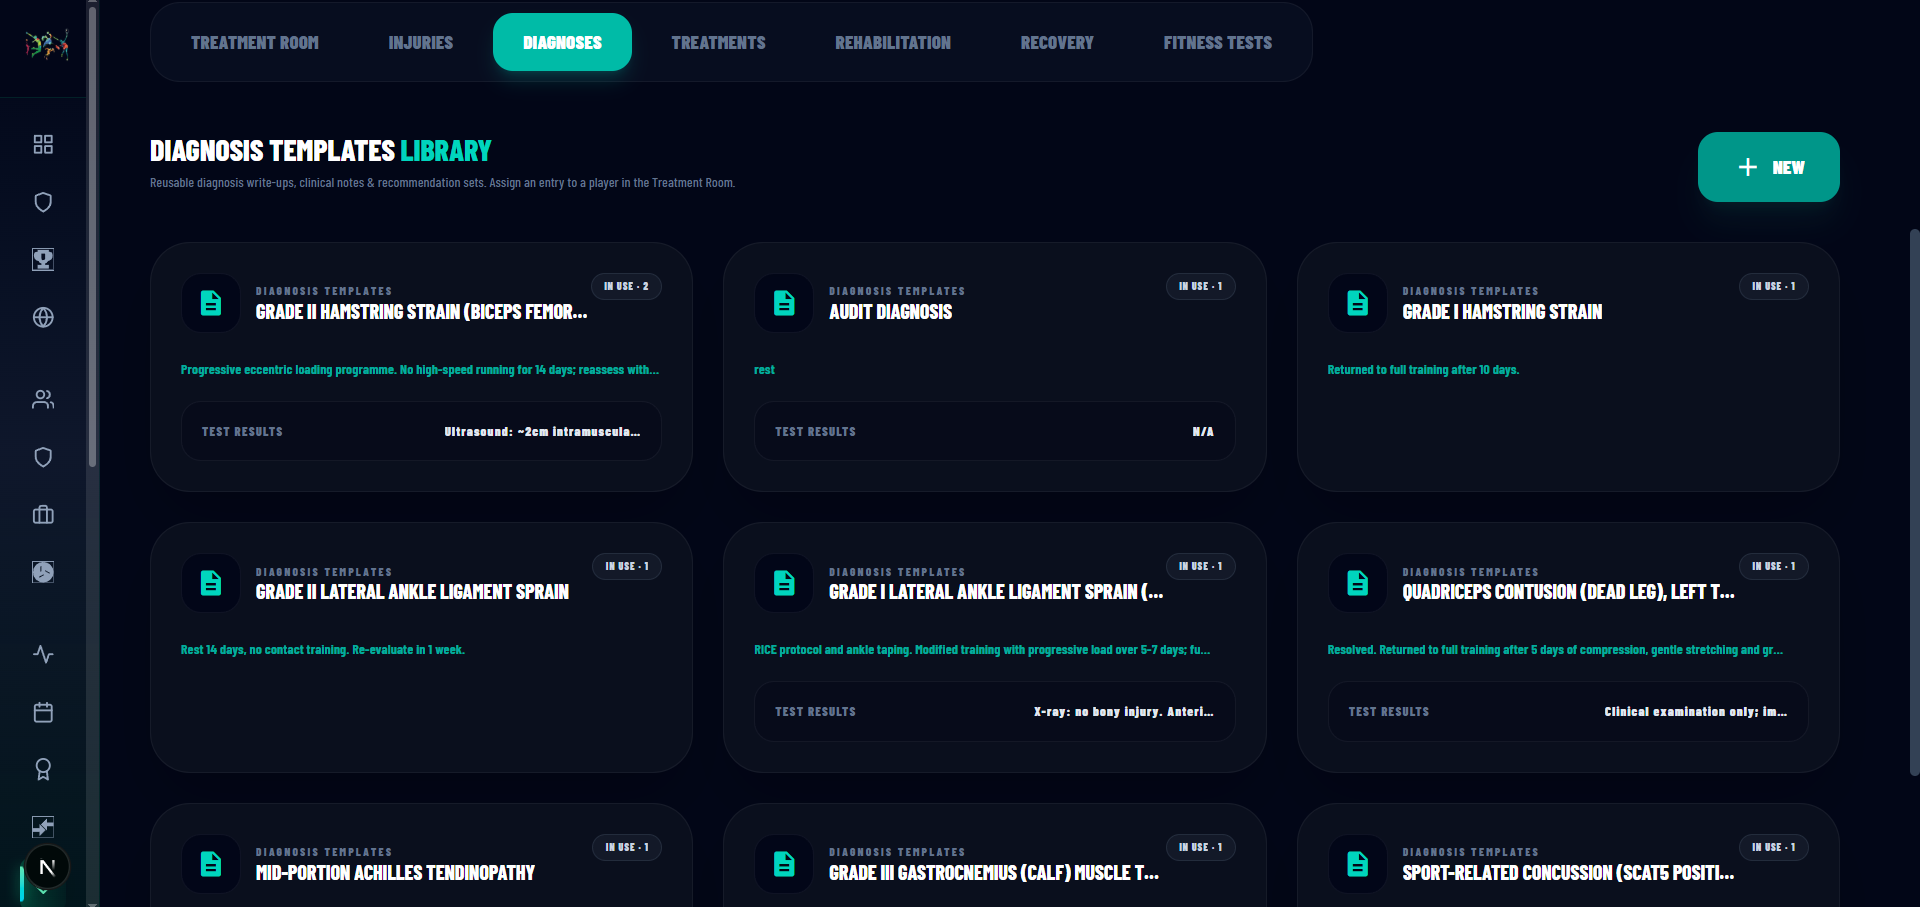
\includegraphics[width=0.95\textwidth]{fig-medical-catalog.png}
  \caption{The general medical catalogs. Reusable injury, diagnosis, treatment,
  rehabilitation, recovery and fitness-test records double as templates that pre-fill the
  journey's stage forms.}
  \label{fig:medical-catalog}
\end{figure}

%======================================================================
\section{Team Communication}
\label{sec:res-messages}

The Messages module delivers a real-time, group-based team chat backed by the notification-mail service
(port~8085). It gives the platform a self-contained communication channel without depending on any third-party
messaging service.

\paragraph{Group and invitation model.} The data model comprises a \texttt{ChatGroup} and a
\texttt{ChatGroupMember}, the latter carrying a membership status (\texttt{INVITED} or \texttt{MEMBER}) that
distinguishes an invited user from a confirmed member. A seeded general group is returned to everyone, while a
user-created group makes its creator a member and places invitees in the invited state until they accept. The chat
group controller is mounted at \texttt{/messages/groups}---a literal path chosen so it takes precedence over the
parameterised \texttt{/messages/\{id\}} route---and exposes the full lifecycle: listing groups, fetching a group and
its members, creating a group, listing a user's pending invitations, and accepting, declining or issuing invitations
through dedicated \texttt{/accept}, \texttt{/decline} and \texttt{/invite} endpoints. The \texttt{Message} entity
carries a \texttt{groupId}, scoping every message to its conversation, and supports threaded replies through a parent
reference.

\paragraph{Reactions and de-duplication.} The conversation supports emoji reactions and client-side de-duplication so
that each message renders exactly once even when it arrives by more than one path (for instance, both echoed over the
socket and returned by a poll). De-duplication is layered: a message is keyed first by its server identifier, then by a
client-assigned message identifier, and finally by the combination of sender and content, which together resolved an
earlier double-render defect.

\paragraph{Real-time delivery over WebSocket.} Delivery is genuinely real-time. A native browser WebSocket connects
directly to the notification service at \texttt{ws://localhost:8085/ws/chat}~\cite{websocket}. The path sits outside the
\texttt{/messages} namespace and outside the gateway deliberately: the raw socket bypasses the gateway's JWT filter and
connects straight to the service, where the endpoint is permitted, which avoids the complications of authenticating a
long-lived socket through the HTTP gateway. The protocol is a small set of JSON text frames. A client first sends an
\texttt{identify} frame carrying its identity; thereafter it sends \texttt{chat} frames carrying the group, sender and
content, which the server re-broadcasts verbatim to every connected client; a \texttt{ping} frame keeps the connection
alive; and the server emits a \texttt{presence} frame on every connect, identify and disconnect, reporting how many users
are online. HTTP polling is retained as a fallback should the socket be unavailable, so the chat continues to function---if
less instantly---even when a WebSocket connection cannot be established (Figure~\ref{fig:messages}).

\begin{figure}[htbp]
  \centering
  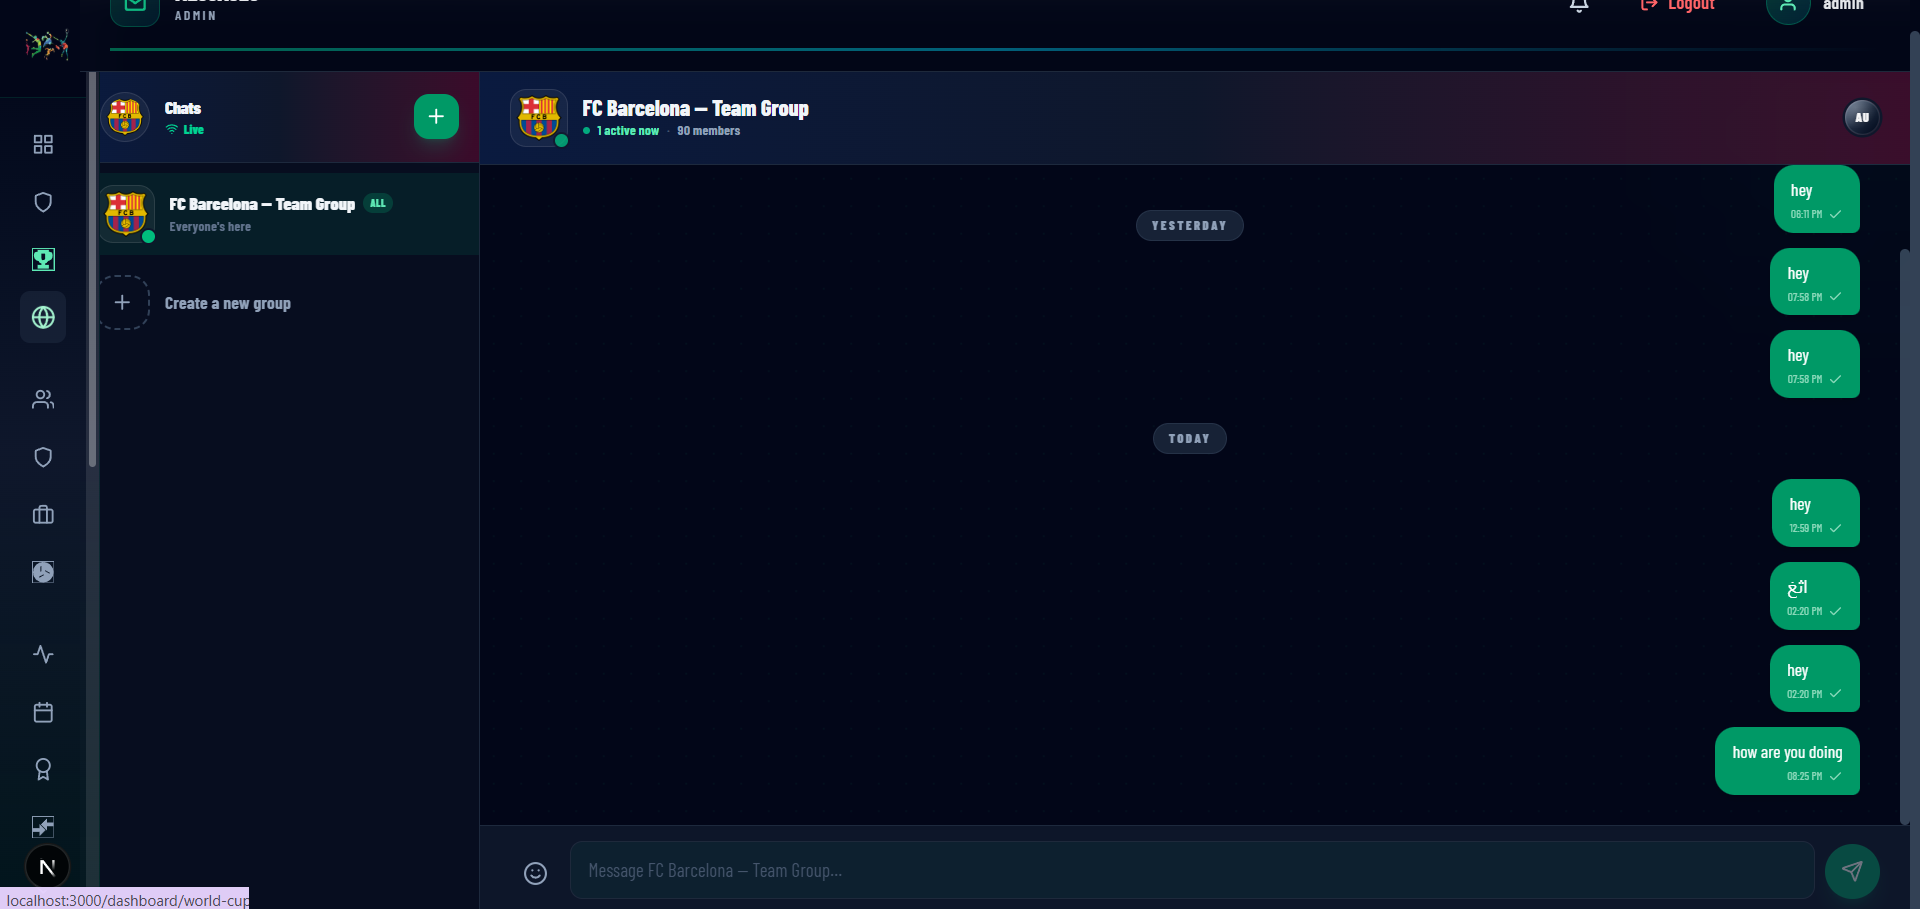
\includegraphics[width=0.95\textwidth]{fig-messages.png}
  \caption{The team group chat. Group conversations, invitations, threaded replies and
  emoji reactions are delivered over a native WebSocket to the notification-mail service,
  with polling as a fallback.}
  \label{fig:messages}
\end{figure}

%======================================================================
\section{Notifications and Alerts}
\label{sec:res-notifications}

Notifications are event-driven and surfaced through a bell in the top navigation bar (Figure~\ref{fig:notifications}).
The notification fabric is one of the clearest expressions of the platform's event-driven, loosely coupled design.

\paragraph{The event pipeline.} The notification-mail service consumes domain events from Kafka~\cite{kafka} through a
set of \texttt{@KafkaListener} consumers, one per topic. When the medical service reports an injury, the player service
completes a transfer, the training service cancels a session, or the match service schedules or completes a match, the
producing service emits an event onto the corresponding Kafka topic following the outbox pattern, and the notification
service's \texttt{EventConsumer} materialises it as a targeted alert with an appropriate type and priority. An injury
event, for instance, becomes an \texttt{INJURY\_REPORTED} alert routed to medical staff, with the priority derived from
the injury's severity; a transfer event becomes a \texttt{TRANSFER\_COMPLETED} alert and may additionally trigger an email
to the affected player. The live-match engine contributes alerts directly over HTTP rather than through Kafka, posting a
goal alert as the match unfolds and a result-available alert when it ends. The alert type enumeration is correspondingly
broad, spanning medical, performance, match-and-training, player-management and scouting-and-sponsorship categories.

\paragraph{The notification centre.} The bell opens a notification centre that presents alerts across two tabs,
distinguishes alerts from notifications, carries unread badges, and refreshes on a short polling interval (on the order of
a few seconds) so that critical events reach the relevant actor promptly. Competition fixtures deep-link from the
notification and competition surfaces into the match-creation flow, pre-filling the teams and carrying the originating
fixture's identity so that scheduling a match from an alert requires no re-entry of detail. This realises the role-aware
notification fabric called for in the requirements and removes the reliance on ad-hoc, manual alerting.

\paragraph{Why event-driven.} Routing notifications through Kafka rather than direct service-to-service calls is what keeps
the producing services ignorant of who consumes their events. The medical service does not know that an injury produces an
alert, an email and a player withdrawal; it simply records the injury and emits a fact. New consumers can be added without
touching the producers, which is the loose coupling the microservice architecture set out to achieve.

\begin{figure}[htbp]
  \centering
  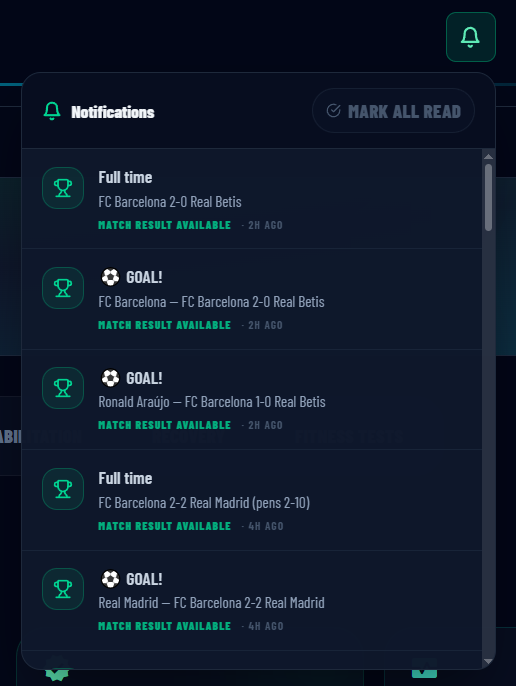
\includegraphics[width=0.9\textwidth]{fig-notifications.png}
  \caption{The notification centre opened from the top-bar bell. Alerts are generated
  automatically from Kafka domain events and from the live-match engine, tagged by role and
  unread state.}
  \label{fig:notifications}
\end{figure}

%======================================================================
\section{Training}
\label{sec:res-training}

The Training module presents the club's training schedule as managed by the training-match service, covering sessions,
plans, drills, attendance and post-session assessments (Figure~\ref{fig:training}).

\paragraph{User experience.} Sessions are displayed on a schedule with a \emph{live-now} indicator that highlights a
session currently in progress, computed from the session's scheduled window in the same timestamp-driven manner as the
match countdown. Plan-driven training ties drills to ratings, attendance and completion tracking, so a session is not a
bare calendar entry but a structured plan whose execution can be recorded: which drills were run, who attended, how each
drill was rated and whether the plan was completed.

\paragraph{Integration with availability.} Because the medical module withdraws injured players from training
automatically---again through the shared player status field---the training schedule always reflects the squad's true
availability, and an injured player cannot be marked present at a session he is medically barred from. When a session is
cancelled, the event flows onto Kafka and the notification fabric raises a training-cancelled alert, so the cancellation
reaches the affected staff and players without a separate announcement step. This connects training to the medical and
notification domains rather than leaving it as an isolated calendar.

\begin{figure}[htbp]
  \centering
  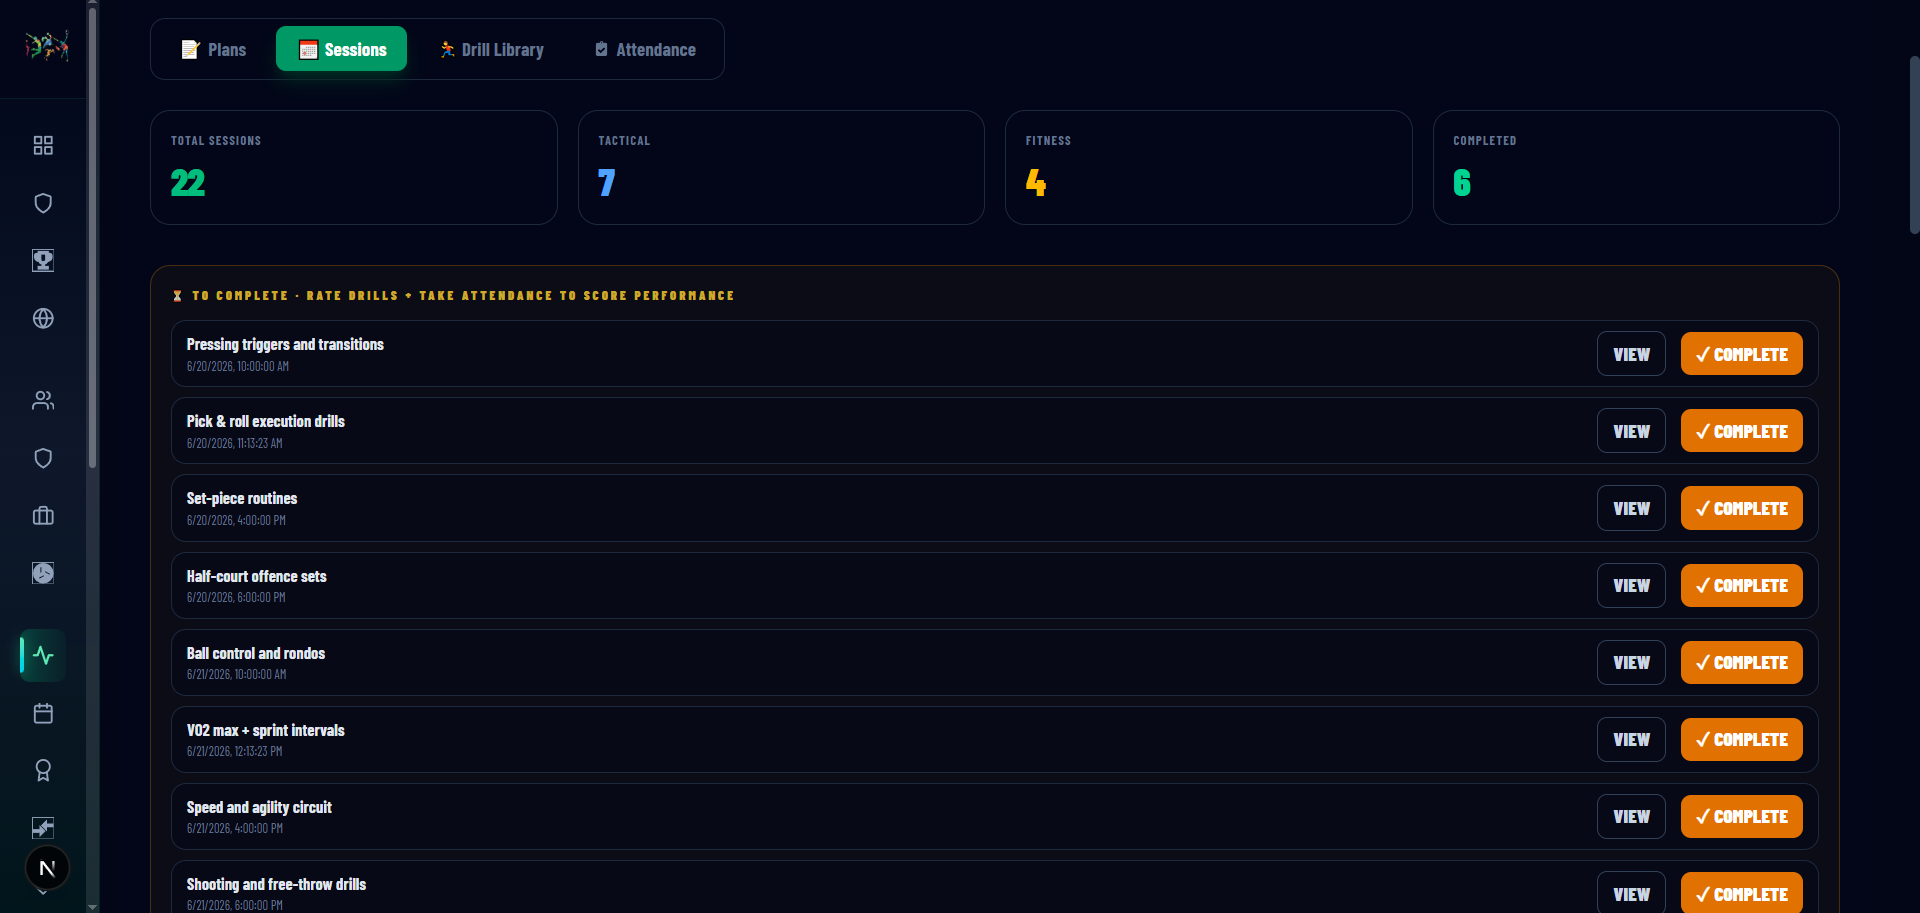
\includegraphics[width=0.95\textwidth]{fig-training.png}
  \caption{The training schedule with a live-now indicator, showing plan-driven sessions
  with drills, attendance and completion tracking.}
  \label{fig:training}
\end{figure}

%======================================================================
\section{Scouting}
\label{sec:res-scouting}

The Scouting module supports the club's recruitment workflow, allowing scouts to record prospect reports against
detailed scouting fields and to route findings to the sport manager for consideration (Figure~\ref{fig:scouting}).

\paragraph{Realisation and integration.} A scouting report captures structured attributes of a prospect rather than
free prose, which makes reports comparable and searchable instead of opaque. When a report is submitted it can raise a
scout-report alert to the sport manager through the same notification fabric, so a finding does not languish unread in an
inbox. Reports feed the transfer and analytics surfaces, providing the audit trail that traditional email-and-PDF scouting
processes lack and connecting the recruitment pipeline to the rest of the platform: a prospect assessed by a scout, transferred
by the player service and analysed by the reports service is the same identity throughout, correlated by the canonical
\texttt{keycloakId}.

\begin{figure}[htbp]
  \centering
  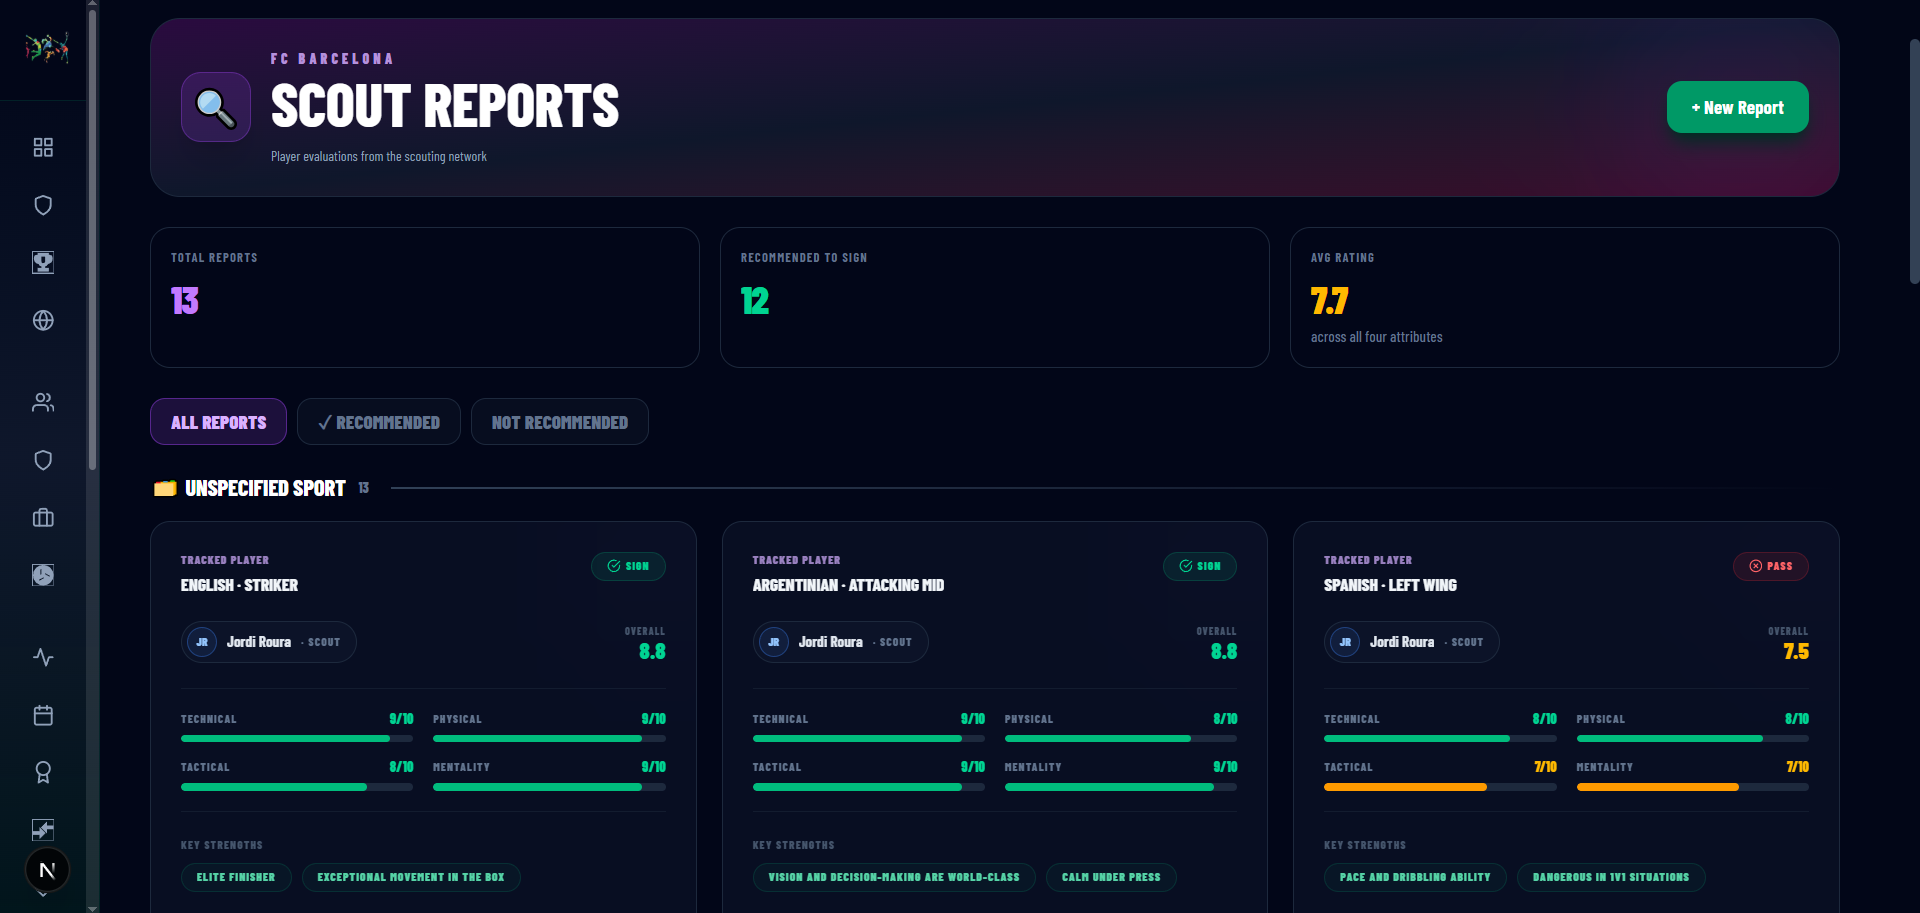
\includegraphics[width=0.95\textwidth]{fig-scouting.png}
  \caption{The Scouting module, where scouts record prospect reports against structured
  fields for review by the sport manager.}
  \label{fig:scouting}
\end{figure}

%======================================================================
\section{Sponsors}
\label{sec:res-sponsors}

The Sponsors module digitises commercial negotiations (Figure~\ref{fig:sponsors}).

\paragraph{Realisation.} Sponsor offers and contract terms are captured as structured records that move through a
negotiation workflow, replacing the opaque email threads of traditional practice with an auditable, notification-generating
process. An incoming offer can raise a sponsor-offer alert to the relevant commercial roles, and decisions taken on an offer
are likewise surfaced through the platform's notification fabric, so the commercial pipeline is integrated with the rest of the
system rather than conducted out of band. The structured representation also means the state of a negotiation is always
explicit---which terms are on the table and where each offer stands---instead of being reconstructed from a thread of
correspondence.

\begin{figure}[htbp]
  \centering
  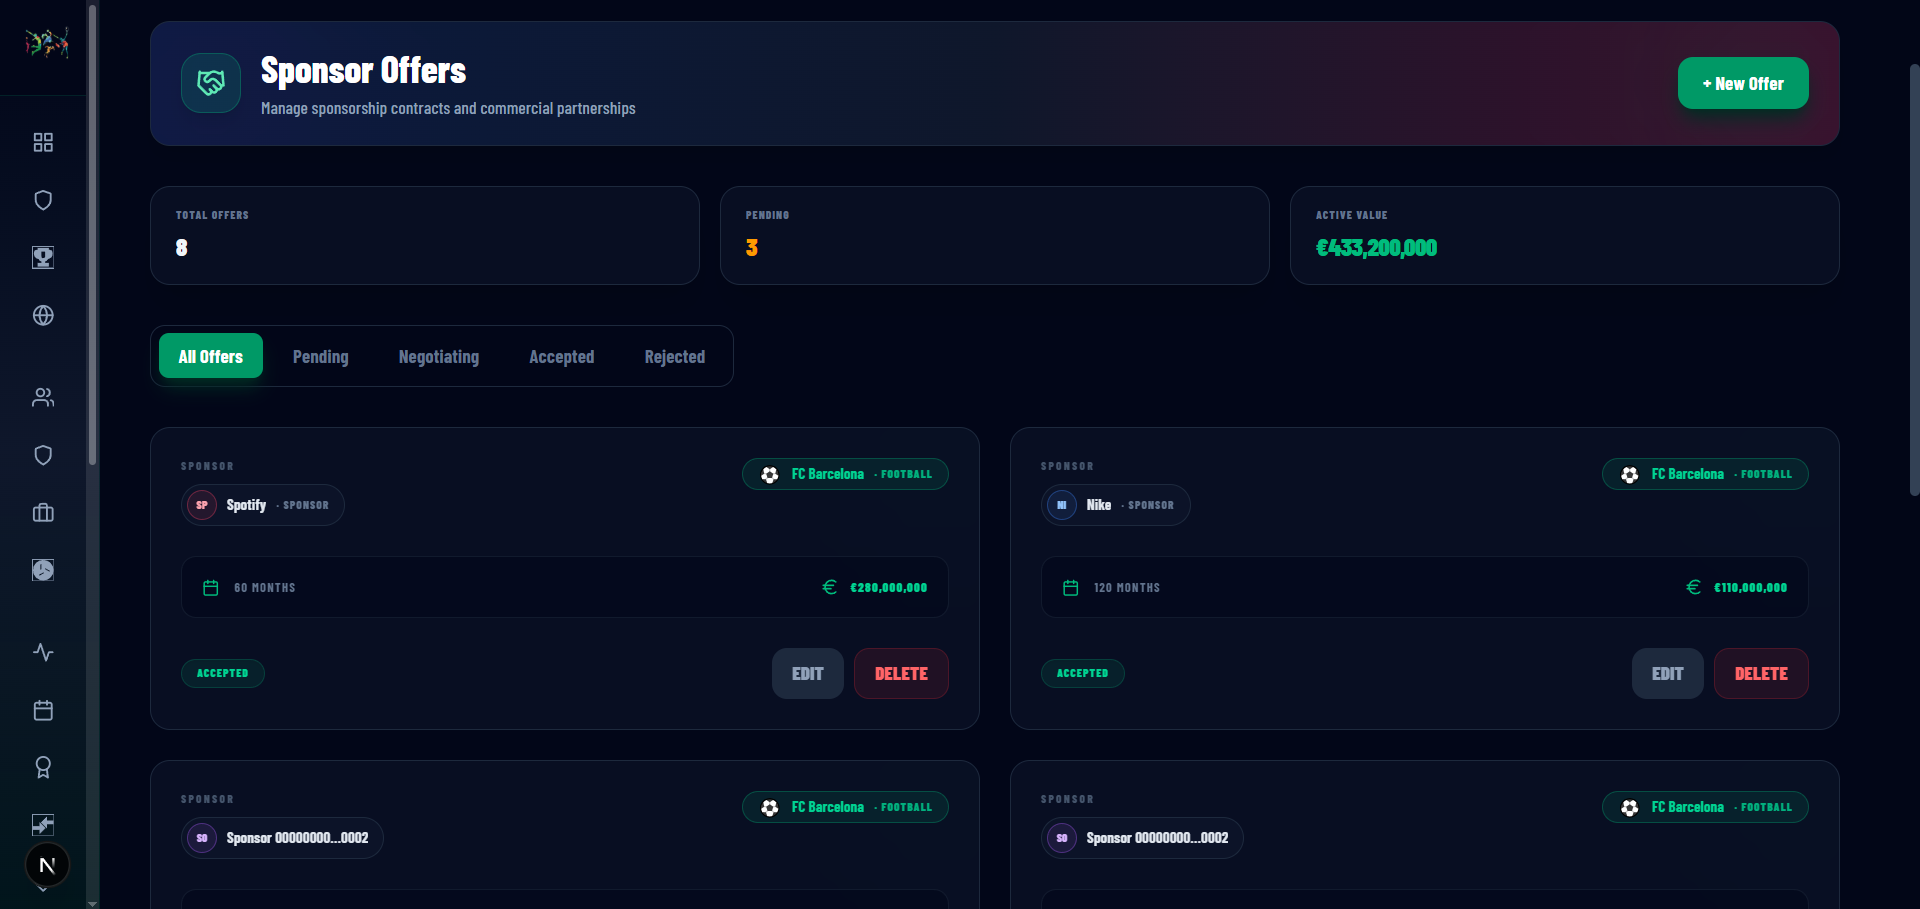
\includegraphics[width=0.95\textwidth]{fig-sponsors.png}
  \caption{The Sponsors module, presenting sponsor offers and contract negotiation as
  structured, auditable records.}
  \label{fig:sponsors}
\end{figure}

%======================================================================
\section{Reports and Analytics}
\label{sec:res-reports}

The Reports module, served by the reports-analytics service (port~8083), aggregates data from across the platform into
match analyses, team- and player-level analytics and training analytics (Figure~\ref{fig:reports}).

\paragraph{Cross-domain insight.} By unifying the previously siloed domains behind a single analytics layer, the module makes
cross-domain insight practical---for example relating match performance to squad availability or training load, a question
that is impossible to answer when each domain lives in its own spreadsheet. The service reads from the operational services'
data and presents the results through role-aware report views, so a performance analyst, a sport manager and a head coach each
see the analyses pertinent to their responsibilities. Because every domain shares the canonical identity scheme, a player's
match statistics, medical history and training attendance can be correlated into a single analytical picture without brittle
name-matching across systems.

\begin{figure}[htbp]
  \centering
  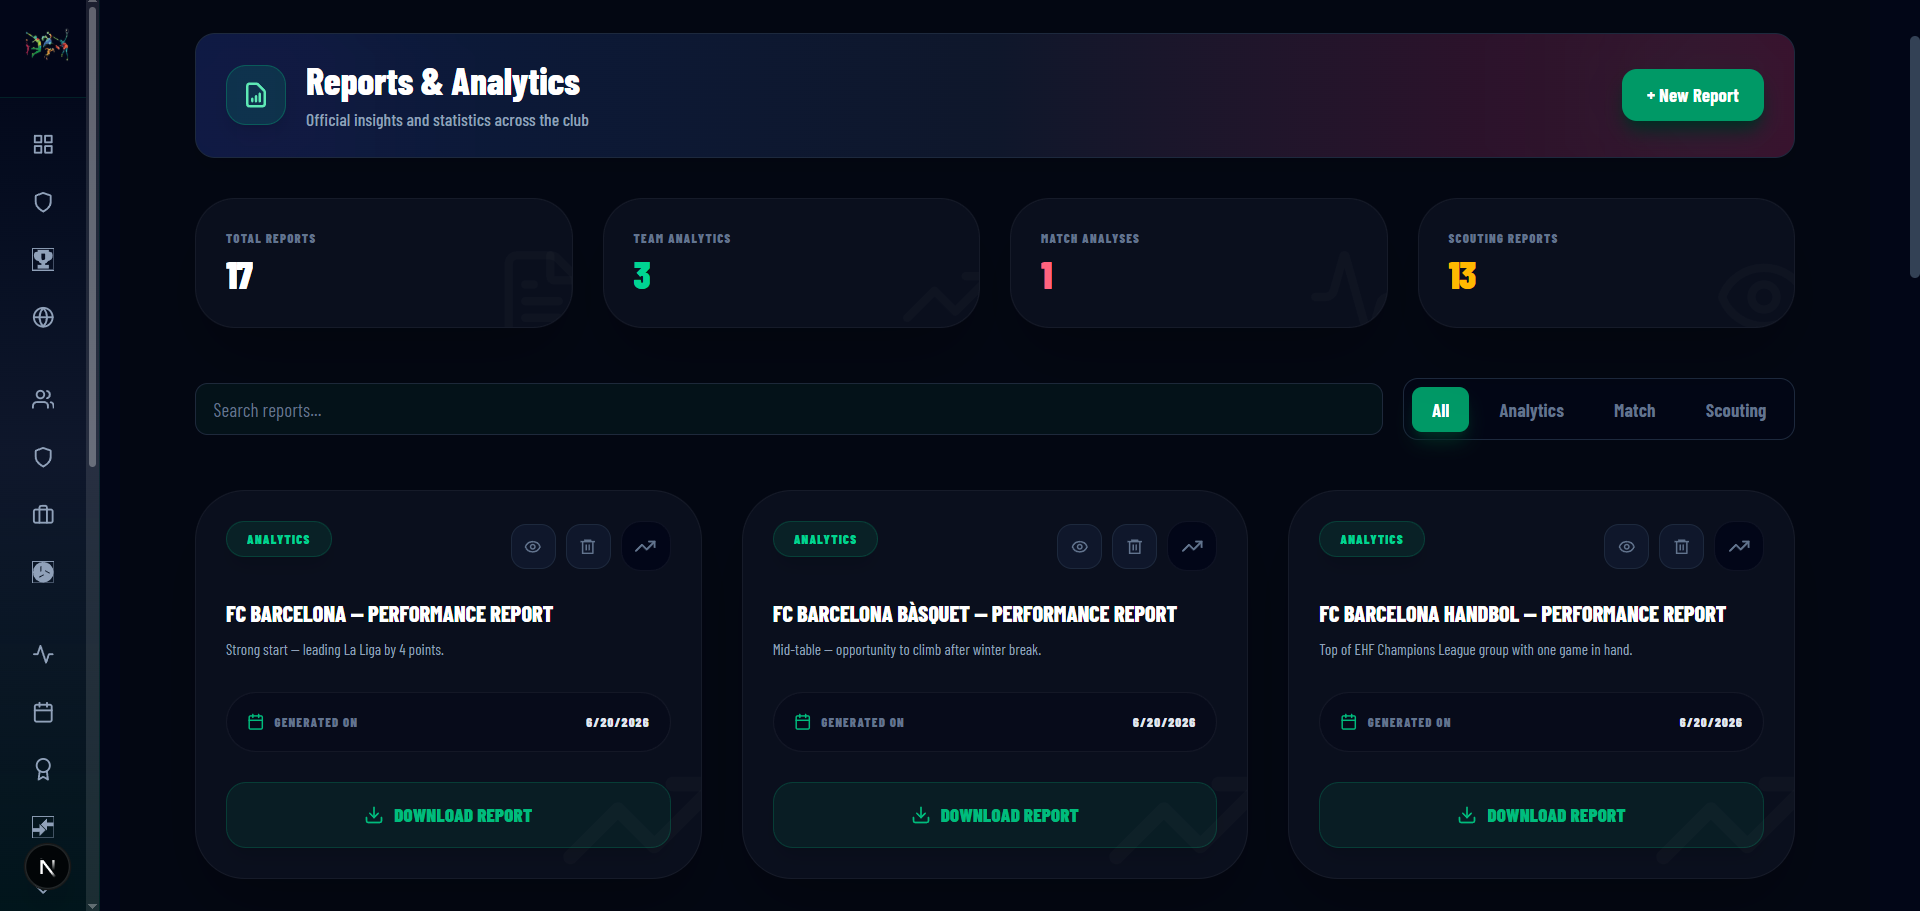
\includegraphics[width=0.95\textwidth]{fig-reports.png}
  \caption{The Reports and Analytics module, aggregating match, team, player and training
  data served by the reports-analytics service.}
  \label{fig:reports}
\end{figure}

%======================================================================
\section{Settings}
\label{sec:res-settings}

The Settings module gives every user control over their profile, preferences, notification choices and security, with changes
genuinely persisted rather than held only in the browser (Figure~\ref{fig:settings}).

\paragraph{Persisted preferences.} Profile, preference and notification settings are saved per user so that the experience is
consistent across sessions and devices. A user's notification choices govern which alerts they receive, and their preferences
shape the interface, both surviving a logout and a change of machine because they are stored server-side rather than in
\texttt{localStorage}.

\paragraph{Keycloak-verified password change.} The security tab supports a password change that is genuinely authoritative
across the platform, because it is mediated by the identity provider rather than by any local store. The change is a two-step
operation handled by the user-management service. First, the user's \emph{current} password is re-verified: the service performs
an OAuth password-grant against the \texttt{mscms} realm using the supplied username and current password, and treats the change
as authorised only if the grant returns an access token. A wrong current password causes the grant to fail with an
invalid-grant error, which the service interprets as a failed verification and rejects the change---so a stolen, unlocked
session cannot silently change the credential without knowing the existing password. Second, only after that verification
succeeds is the new password applied through the Keycloak administrative API. Because the credential lives in the identity
provider, the change takes effect uniformly everywhere the platform authenticates, with no local password copy to fall out of
sync.

\begin{figure}[htbp]
  \centering
  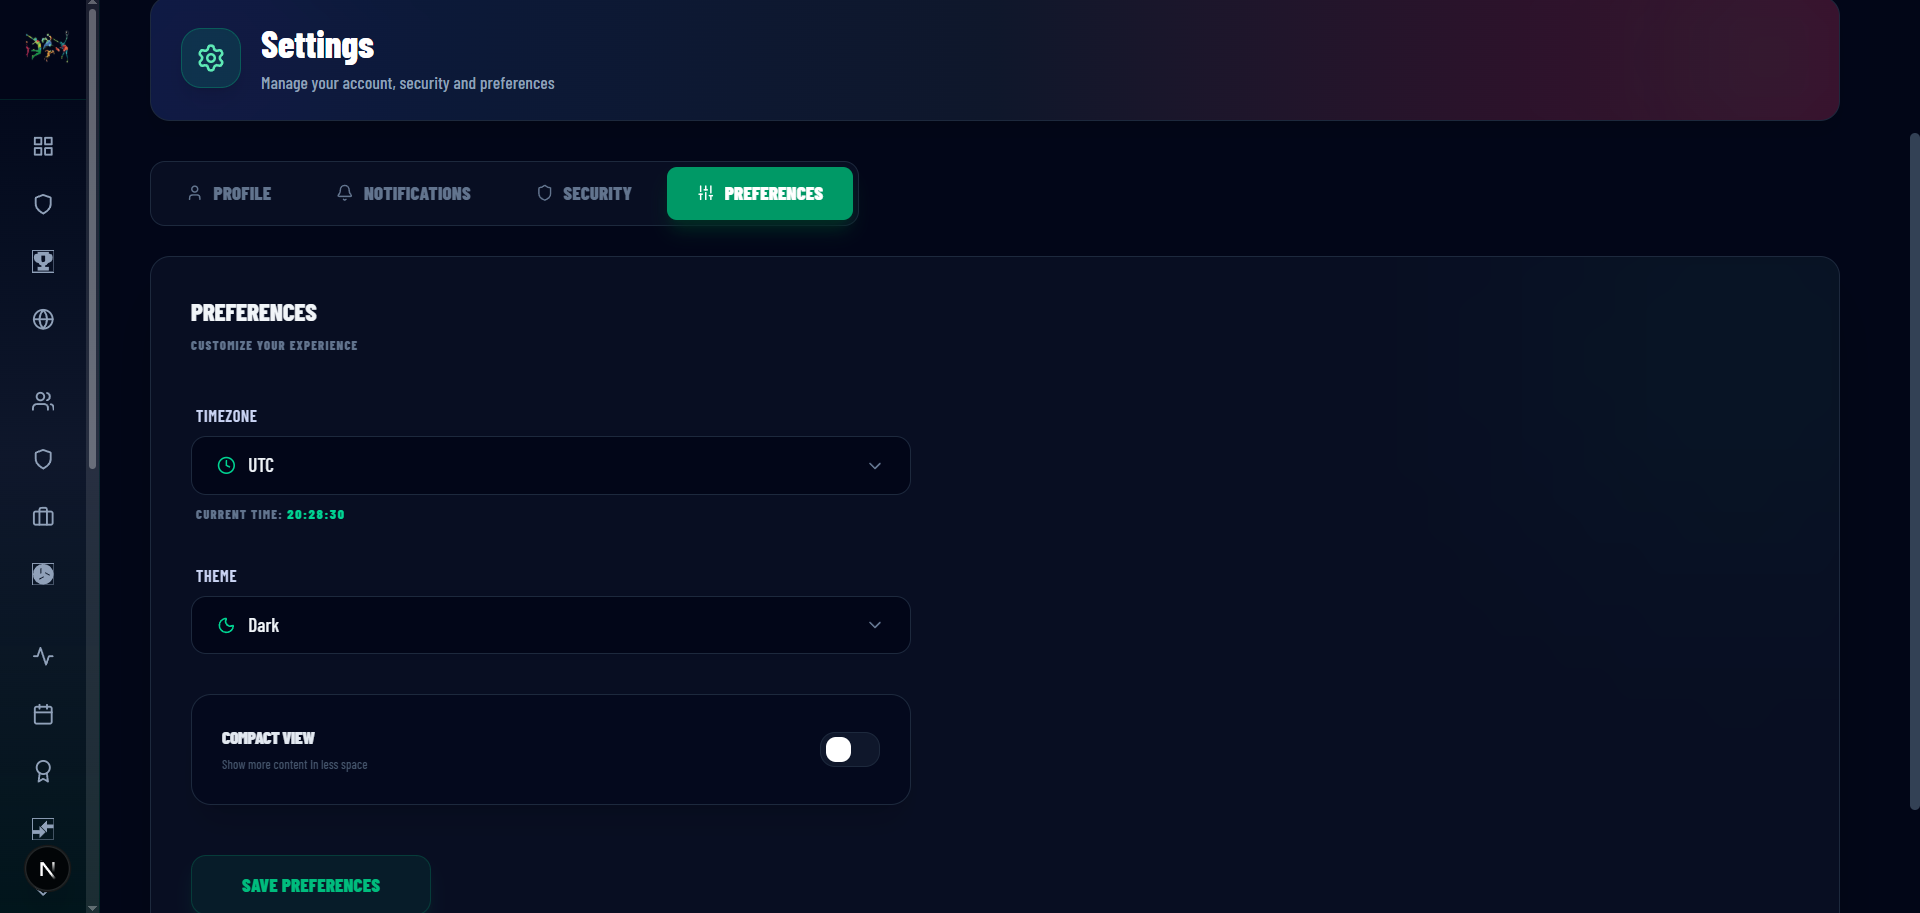
\includegraphics[width=0.95\textwidth]{fig-settings.png}
  \caption{The Settings module, with profile, preferences, notification and security tabs.
  Password changes are verified and applied through Keycloak.}
  \label{fig:settings}
\end{figure}

%======================================================================
\section{Analysis and Evaluation}
\label{sec:res-analysis}

Having presented the implemented modules, this section steps back to evaluate the delivered system as a whole: how completely it
satisfies the functional and non-functional requirements set out in Chapter~2, which design decisions proved most effective,
what the system's performance and user experience are like in practice, and how the implementation was tested and validated.

\subsection{Functional Requirements Coverage}
The implemented system satisfies the functional requirements across every domain identified in Chapter~2.
Authentication, role-based access and the role-aware dashboard realise the identity and onboarding
requirements~\cite{keycloak,jwt,rbac}. The squad, competition and match modules realise the player and
match-operations requirements, and in several respects exceed the original specification: the live-match engine's
broadcast-style phase machine, with knockout-only extra time and penalty shootouts and phase-bounded event minutes,
and the faithful reproduction of the modern Champions League format with its rotation-generated league phase, go beyond
the basic match recording originally envisaged. The medical module realises the medical-and-fitness requirements with a
complete, status-driven injury lifecycle from report to fitness-cleared recovery. The messages, notifications, training,
scouting, sponsor and reports modules realise the communication, notification and analytics requirements, with the
head-to-head, world-cup and trophy-room surfaces adding fan-facing context beyond the operational core. Crucially, the
consistent enforcement of role-based access at the identity provider, at the gateway and in the front-end
middleware---the three-layer scheme described in Chapter~3---means a permission rule applies uniformly whether a user
navigates the interface or calls the API directly, so the access control is not merely cosmetic.

\subsection{Non-Functional Requirements Coverage}
The non-functional requirements were met chiefly through architectural choices rather than after-the-fact tuning.
\emph{Maintainability and modularity} are served by the decomposition into six independently deployable services behind a
gateway and a service registry, each owning its own database, so a change to the medical schema cannot break the match
service. \emph{Security} is centralised in Keycloak and enforced at three layers, with no service trusting anything but a
validated token, and with the most sensitive operation---a password change---re-verifying the current credential before
proceeding. \emph{Scalability and loose coupling} follow from the event-driven notification pipeline: producers emit facts
to Kafka and remain ignorant of consumers, so the system can grow new reactions to existing events without modifying the
producers. \emph{Reliability} is supported by idempotent ingestion (de-duplicated by external identifier), the self-cleaning
Match Hub, and graceful degradation on the dashboard where one slow service suppresses only its own card. \emph{Usability}
is addressed by the single-origin API client, the automatic recovery on token expiry, and the timestamp-driven live clock and
countdowns that keep the interface responsive without server round-trips.

\subsection{Design Decisions That Worked Well}
Several decisions proved especially effective in practice. Making the back-end the single source of truth for external data,
with scheduled idempotent ingestion and read-through standings, kept the front-end simple and the data trustworthy while
respecting the data provider's free-tier constraints and never exposing the API key to the browser. Capturing the lineup
atomically with the match guaranteed that every match carries a reconstructable starting XI, which is precisely what makes the
live engine, the substitution logic and the match-details page meaningful rather than synthetic. Deriving the medical journey's
current stage solely from the injury status produced a workflow that is immune to leftover records and easy to reason about, and
allowing an in-match injury event to create a real medical record and withdraw the player demonstrated genuine, end-to-end
cross-service integration spanning the match, player and medical services in a single action. Resolving the knockout-versus-points
decision from the originating fixture's round, rather than from a loose match type, kept the live engine consistent with the
competition format. Finally, the event-driven notification fabric, fed by Kafka and the live engine, delivered the role-aware
alerting the requirements demanded with no manual intervention.

\subsection{Performance and User-Experience Observations}
The microservice decomposition allowed each domain to be developed and reasoned about in isolation, and routing every browser
request through a single gateway origin kept the API client and the cross-origin configuration straightforward~\cite{microservices,restapi}.
The live clock and countdown are computed from pure timestamp helpers, so the common case of simply advancing the clock incurs no
server round-trip and the live view stays responsive, while every state-changing action is persisted immediately so that a reload
faithfully reconstructs the match---including the on-pitch set, the consumed substitutions and the running phase. The dashboard's
parallel, per-card aggregation keeps perceived latency close to that of the slowest single dependency rather than the sum of all
of them. The self-cleaning Match Hub and the status-driven medical and squad logic markedly reduce the manual reconciliation that
burdens traditional tools, since a single status change propagates everywhere it is relevant. Two classes of defect encountered
during development are worth recording because their fixes shaped the design: a timezone-conversion bug that made matches appear
hours early was resolved by storing and parsing kickoff times as naive local wall-clock values, and a clock that could inflate into
nonsensical added time (an observed ``45+132''') was resolved by hard-capping the displayed minute at the phase length and showing
only admin-set stoppage. The principal real-world limitation observed is external rather than architectural: because the modelled
system date sits after the imported seasons' conclusion, the freely available data contains no upcoming or in-progress fixtures, so
live ingestion of genuinely new matches will populate only once a new season is published. The platform nonetheless demonstrates the
full live and ingestion machinery against the schedulable, club-created matches, and the ingestion pipeline will auto-fill league
fixtures when a new season appears in the provider's data.

\subsection{Testing and Validation Approach}
Validation combined automated and manual techniques appropriate to a system of this size. At the back-end, the domain services
carry controller-level tests---for example, tests around the match-event, match-formation and match-lineup controllers in the
training-match service and the injury and message controllers in the medical and notification services---that exercise the REST
surface and the entity mappings. The most behaviourally complex logic was deliberately structured as pure functions to make it
unit-testable in isolation: the live-clock and phase-machine helpers (phase derivation from a minute, phase-bounded recordable-minute
ranges, the stoppage-capped clock label, and the kickoff validator) take only timestamps and configuration and return deterministic
results, so their many edge cases---a minute past regulation, a knockout tie level at full time, a kickoff in the past or under the
five-minute lead---can be asserted directly. The fixture generators are likewise deterministic: the double round-robin and the
Champions League rotation algorithm produce the same fixture graph for the same input, which makes properties such as ``every team
plays exactly eight distinct opponents'' and ``no pairing repeats'' verifiable. Beyond automated tests, the system was validated by
end-to-end exercise of the user journeys against the running, containerised stack: provisioning a user through Keycloak and signing
in, creating a competition and confirming the generated fixtures, scheduling a match with a mandatory lineup, driving a live match
through its phases including a knockout tie into penalties, triggering an in-match injury and following the player through the
medical journey to a cleared fitness test, exchanging real-time chat messages over the WebSocket, and confirming that the resulting
Kafka-driven and live-engine alerts appeared in the notification centre. A noted constraint on this process was that automated
screenshot-based visual verification could not attach to the developer's running instance, so visual changes were validated by
inspecting routes, bundles and live-API behaviour and by manual review of the rendered interface, while behavioural correctness was
established through the automated tests and the end-to-end journeys described above.

\subsection{Summary}
Taken together, the modules presented in this chapter show that the platform delivers on its central promise: to consolidate the
fragmented operational concerns of a multi-sport club into a single, role-aware, cloud-native system in which match operations,
medical care, communication, recruitment, commercial activity and analytics are connected rather than siloed. The combination of a
real, idempotent ingestion pipeline, a behaviourally faithful live-match engine, a status-driven clinical injury workflow, a
real-time WebSocket communication channel and an event-driven notification fabric distinguishes the delivered system from the simple
CRUD application from which it evolved, and substantiates the design objectives stated at the outset of this report. The evaluation
above confirms that the functional and non-functional requirements of Chapter~2 are met or exceeded, and identifies the small number
of limitations---chiefly the post-season external data and the constraints on automated visual verification---that bound the present
implementation and motivate the future work discussed in the next chapter.

\chapter{Conclusions and Recommendations}
\label{ch:conclusion}

This final chapter draws together the work presented in the preceding chapters. It first
states the overall conclusion of the project and situates it against the objectives set out
in Chapter~\ref{ch:introduction}; it then itemises in detail what was actually delivered;
it reflects on the technical and teamwork lessons that emerged during development; it
discusses the system's honest limitations without overstating its maturity; and it finally
sets out a prioritised programme of future work and recommendations. Taken as a whole, the
chapter is intended to serve two audiences: an assessor seeking a candid appraisal of the
degree to which the project met its goals, and a future maintainer seeking a clear sense of
where the platform stands and where it could profitably be taken next.

\section{Conclusion}
\label{sec:conclusion-summary}

The objective of this graduation project was to design and build a single, coherent,
cloud-native platform that consolidates the fragmented operational concerns of a
multi-sport club into one secure and analytically rich system. Taking FC~Barcelona as
the working organisational model and \textit{Sportify} as the product brand, the
project set out to replace the patchwork of spreadsheets, e-mail threads and
disconnected SaaS tools described in Chapter~\ref{ch:introduction} with a unified platform
on which each professional role---from leadership through coaching, medical, scouting and
commercial staff down to players and fans---sees exactly the information relevant to its
responsibilities, and nothing more. The thesis underpinning the work was that the
structural problems of club management---data fragmentation, multi-discipline complexity
and analytical blindness---are not problems of any single feature but of architecture, and
that a properly decomposed, identity-centred, event-driven system could dissolve them at
their root.

This objective was met. The Multi-Sport Club Management System (MSCMS) is a working
platform built on a microservices architecture~\cite{microservices} of six domain
services and a three-part control plane---together seven independently deployable
Spring~Boot~3.5.6 / Java~21 services~\cite{springboot}---discovered through Eureka and
reached through a single Spring Cloud Gateway~\cite{springcloud}, fronted by a
Next.js~16 / React~19 application~\cite{nextjs,react}, and orchestrated as containers
through a single Docker~Compose stack~\cite{docker}. Every request is authenticated against
a Keycloak realm and verified as a JSON Web Token at the gateway~\cite{keycloak,jwt}, and
persistence follows the database-per-service pattern over PostgreSQL~\cite{postgres} with
asynchronous, event-driven coordination over Apache~Kafka~\cite{kafka}. The architectural
hypothesis was therefore not merely asserted but demonstrated in running software: each of
the structural problems identified at the outset is answered by a concrete architectural
mechanism---fragmentation by a shared identity and a single gateway origin, multi-discipline
complexity by sport-aware domain models, and analytical blindness by a reporting service
that aggregates across the previously siloed domains.

Beyond reproducing the operational baseline, the project advanced the system from a
predominantly CRUD-oriented tool into a genuinely interactive sports platform. The
headline outcomes are a database-backed competitions module that models La~Liga and the
new-format UEFA Champions League with a single league phase and a knockout bracket, fed by
real fixture data ingested from football-data.org~\cite{footballdata}; a broadcast-style
live-match engine that drives a match through its phases in real time, complete with
extra time and penalty shoot-outs for knockout ties; a clinical injury-management
workflow that follows each injured player through a staged recovery journey; a real-time
team messaging facility built over WebSocket~\cite{websocket}; an event-driven
notification centre; and consistent role-based access control~\cite{rbac} enforced at
identity, gateway and user-interface layers. Collectively, these capabilities
demonstrate that the architectural decisions taken early in the project---service
decomposition, a central identity provider, an asynchronous event backbone and a
REST-based contract between front-end and back-end~\cite{restapi}---scaled gracefully to
accommodate substantially richer behaviour without structural rework. It is worth
emphasising this last point: none of the later, behaviourally complex modules required a
new service, a new gateway route or a change to the authentication model. The competitions
module and the live-match engine were absorbed by the training-match service because they
share the match and line-up schema; the staged injury workflow was absorbed by the
medical-fitness service; and the group chat and alert centre were absorbed by the
notification-mail service, which already owned messages and consumed the events that drive
alerts. That the architecture could grow this much at the leaves while remaining stable at
the trunk is, in the team's assessment, the project's strongest evidence that its founding
design choices were sound.

In short, the system is not a prototype that merely gestures at its intended scope. It is a
runnable, role-aware, secure platform in which the day-to-day operations of a multi-sport
club---squad administration, training, match operations, medical care, recruitment,
commercial negotiation, analytics and fan engagement---are connected through a common
identity and a common data backbone rather than scattered across disconnected tools.

\section{What Was Delivered}
\label{sec:delivered}

The project delivered a complete, runnable multi-sport club management platform whose
principal artefacts are summarised below. The itemisation is deliberately concrete: each
entry names the artefact, its location in the architecture, and the requirement family it
satisfies, so that the claim of completeness can be checked against the requirements
catalogue reproduced in Appendix~A.

\begin{itemize}
  \item \textbf{A microservices back-end.} Seven Spring~Boot services---the six domain
        services user-management, player-management, training-match, medical-fitness,
        reports-analytics and notification-mail, fronted by an API gateway, a configuration
        server and a Eureka service registry---all orchestrated by a single Docker~Compose
        definition alongside Keycloak, PostgreSQL, Kafka, Redis and RabbitMQ. Each domain
        service owns a dedicated database, registers itself for discovery on boot, and
        draws its configuration from the Config Server, so that the entire control plane
        and data plane come up from one reproducible command.

  \item \textbf{Layered identity and access control.} Every request is authenticated
        against the Keycloak \texttt{mscms} realm using the \texttt{keycloakId}
        identifier (the JWT \texttt{sub} claim, never an internal database key), and
        authorisation is enforced consistently at three layers---the identity provider, the
        API gateway and the Next.js route guards---so that the same per-role permission
        rules apply whether a user navigates the interface or calls the APIs directly. The
        front-end permission map is the single source of truth that drives both the
        navigation a user sees and the routes the middleware will admit, eliminating drift
        between what is shown and what is allowed.

  \item \textbf{A real competitions module.} Database-backed competitions modelling
        La~Liga and the new-format UEFA Champions League (a single combined league phase
        followed by a knockout bracket that unlocks only once the league phase concludes),
        with a guided multi-step creation flow, automatic round-robin fixture generation
        for league formats, completed competitions automatically locked as read-only with a
        ``Completed'' badge, and real, finished seasons imported from the football-data.org
        API as seed data. Standings are recomputed from the recorded fixture results rather
        than stored, so the table is always consistent with the matches that produced it.

  \item \textbf{A live-match engine.} A broadcast-style phase machine advancing a match
        through first half, half-time, second half and full time---and, for knockout
        ties, through two periods of extra time and a penalty shoot-out---with the line-up
        locked at creation, phase-bounded and administrator-set stoppage time, per-sport
        substitution limits, in-match event and injury recording, real goal and result
        alerts raised as events occur, and automatic write-back of the final score to the
        source competition fixture. The knockout-versus-points decision is resolved from
        the originating fixture's round, so a draw is correctly permitted for a league-phase
        fixture and correctly disallowed for a knockout tie.

  \item \textbf{A clinical injury-management workflow.} A medical \emph{Treatment Room}
        separating currently-injured from recovered players, with each player advancing
        through a staged journey---injury, diagnosis, treatment, rehabilitation, recovery,
        fitness test and return to fitness---driven by the injury's own status as the single
        source of truth for the current stage. Logging an injury automatically withdraws the
        player from upcoming matches, line-ups and training, and only a passing fitness test
        returns the player to the available pool; the journey is supported by general
        medical reference catalogues for injuries, diagnoses, treatments, rehabilitation,
        recovery programmes and fitness tests.

  \item \textbf{Real-time team messaging.} A group-chat facility built on persistent
        \texttt{ChatGroup} and \texttt{ChatGroupMember} entities, with a seeded general
        group returned to everyone, user-created groups, membership invitations carrying an
        invited-or-member state with explicit accept and decline actions, threaded replies
        and emoji reactions, and client-side de-duplication so each message renders exactly
        once. Delivery uses a native WebSocket channel connected directly to the
        notification service at \texttt{ws://localhost:8085/ws/chat}, deliberately outside
        the gateway's JWT filter, with authenticated polling retained as a resilient
        fallback.

  \item \textbf{An event-driven notification centre.} A top-bar alert bell backed by a
        Kafka consumer that turns domain events---scheduled and completed matches,
        injuries, transfers and cancelled training, together with live-match goal and
        result alerts contributed directly by the live engine---into role-aware,
        priority-tagged notifications. The centre presents alerts and notifications across
        two tabs, carries unread badges, and refreshes on a short polling interval so that
        critical events reach the relevant actor promptly.

  \item \textbf{A polished, role-aware front-end.} A Next.js application providing
        per-role dashboards, a public-facing Club Hub and player profiles with real
        photographs, the competitions and match surfaces described above, aggregated
        analytics and reports, a read-only mode for players and fans, and a settings area
        with real persistence and a Keycloak-verified password-change flow, all presented
        under the \textit{Sportify} brand identity. Auxiliary surfaces such as a head-to-head
        record view and a real FIFA World Cup view, computed entirely from back-end data,
        round out the consumer-facing experience.

  \item \textbf{Project documentation and deployment assets.} Alongside the running code,
        the project delivered an entity-relationship description of the six databases, an
        authentication sequence description, a complete features-and-endpoints reference, a
        Docker quick-start guide, and the prebuilt-image build workflow that allows the
        stack to be assembled reproducibly on a host where in-container Maven cannot reach
        the network. The deployment and run procedure is reproduced in Appendix~E.
\end{itemize}

\section{Lessons Learned}
\label{sec:lessons}

Developing a distributed system of this scope as a student team yielded several
durable lessons, both technical and organisational. They are recorded here not as
platitudes but as concrete observations that changed how the team worked.

\paragraph{Contract drift is the dominant cost of distributed development.}
The single most expensive recurring problem was the drift between the front-end client,
the back-end data-transfer objects and the database schema. A field renamed on one side,
or a status value spelled differently across services, repeatedly produced silent
failures that were costly to trace because no single component was obviously at fault: the
front-end believed it was sending the right shape, the back-end believed it was receiving
the wrong one, and the only evidence was an empty list or a swallowed error. The team
mitigated this by nominating a single source of truth for each cross-cutting concern---for
example a shared permissions module on the front-end and seed-identifier constants on the
back-end---and by treating the REST contract~\cite{restapi} as a deliberate interface
rather than an incidental byproduct of implementation. The broader lesson is that in a
distributed system the interface between components deserves at least as much design care as
the components themselves.

\paragraph{Asynchronous, event-driven design pays for itself as features grow.}
Adopting a Kafka event backbone~\cite{kafka} early meant that later features such as
the notification centre and live-match alerts could be added by consuming events already
being published, rather than by threading new synchronous calls through multiple
services. When the live-match engine needed to announce a goal or a final result, it did
not need to know who cared---it published an event, and the notification service, which
already consumed the domain's event stream, turned it into an alert. This validated the
decision to favour loose coupling and demonstrated, in practice, why event-driven
microservices~\cite{microservices} scale better with feature count than a tightly coupled
design: the cost of adding a consumer is independent of the number of producers.

\paragraph{Centralised identity simplifies everything downstream.}
Delegating authentication to Keycloak~\cite{keycloak} and propagating identity as a
signed JWT~\cite{jwt} removed an entire class of problems---password storage, session
handling and per-service user tables---and made the three-layer RBAC~\cite{rbac} model
tractable. Because every service trusts the same signed token and refers to a person by the
same \texttt{keycloakId}, identity never had to be reconciled across service boundaries.
The lesson was that investing in a single identity provider before building features,
rather than retrofitting one later, repaid the effort many times over; the two-step,
Keycloak-verified password change is a small but telling example of the leverage this
gained, since the same provider that issues tokens also authoritatively re-verifies the
current credential before allowing it to change.

\paragraph{Idempotent, deterministic seeding makes a distributed system safe to operate.}
Guarding every seeding routine so that it runs only against an empty store, and preserving a
deterministic insertion order so that cross-service numeric identifiers remain stable, made
the full stack safe to tear down and redeploy without corrupting data. This proved
indispensable when iterating across seven services with independent databases: the team
could wipe the volumes, bring the stack back up, and rely on a consistent baseline in which
FC~Barcelona always carried the same team identifier in every service that referenced it.

\paragraph{A container-first discipline removes a whole category of integration pain.}
Running every service through Docker~Compose from the earliest iterations~\cite{docker}
eliminated the ``works on my machine'' class of defect and gave every iteration a
reproducible integration environment. The discovery that in-container Maven could not reach
the network on the development machine forced a prebuilt-image workflow---building fat jars
on the host and copying them into minimal runtime images---which, although born of a
constraint, ultimately produced faster, more predictable rebuilds.

\paragraph{Teamwork lessons.}
Working as a multi-person team across loosely coupled services, an agile, iterative
process~\cite{agile} with short cycles and frequent integration was essential: the
team learned to agree interface contracts before parallel work began, to integrate often
rather than at the end, and to keep shared documentation and conventions current so that
a service owned by one member could be safely consumed by another. Clear ownership of
each service, combined with disciplined communication at the integration boundaries,
was the practical key to progressing in parallel without constant blocking. The team also
learned the value of a vertical-slice habit---finishing each iteration with an integrated,
runnable system rather than a drawer of disconnected parts---because it surfaced
integration problems while they were still small and cheap to fix.

\section{Limitations}
\label{sec:limitations}

In the interest of an honest appraisal, the system carries a number of limitations that a
production deployment would need to address. These are stated plainly; none of them
undermines the project's central claim, but each marks a boundary between what was built and
what a fully operational product would require.

\begin{itemize}
  \item \textbf{Single-region, single-host deployment.} The platform runs as a single
        Docker~Compose~\cite{docker} stack on one host. There is no clustering,
        horizontal autoscaling or multi-region redundancy, so the current deployment is
        appropriate for demonstration and evaluation rather than high-availability
        production use. The architecture is designed to permit horizontal scaling---each
        service is stateless behind the gateway and discoverable through Eureka---but that
        capability has not been exercised against a real orchestrator.

  \item \textbf{Manual operational tasks.} Several operational steps remain manual,
        including building service artefacts on the host before image assembly and the
        manual triggering of certain data-synchronisation tasks. There is no continuous
        integration or deployment pipeline, and observability is limited to container
        logs rather than dedicated metrics, dashboards and distributed tracing, which makes
        diagnosing a cross-service problem more laborious than it would be in a mature
        operational setup.

  \item \textbf{Client-side medical reference templates.} The general medical
        catalogue templates that support the injury workflow are partly held on the client
        rather than being fully persisted server-side, which means they are not yet
        centrally managed or shared consistently across sessions and users. The per-player
        clinical records themselves are persisted; it is the reusable template library that
        is incompletely server-backed.

  \item \textbf{Constraints of the external data feed.} Because real fixture data is
        drawn from the free tier of football-data.org~\cite{footballdata}, the system
        is limited to the competitions and seasons that tier exposes; team-scoped endpoints
        are forbidden on the free tier, so the service reads competition-scoped endpoints
        instead. At the project's reference date the available data is post-season and
        therefore consists of finished matches, so the live-match engine is best
        demonstrated on manually created fixtures rather than on genuinely upcoming
        real-world ones.

  \item \textbf{Approximated real-time presence.} Real-time messaging operates over a
        WebSocket channel~\cite{websocket} with a polling fallback, but the system does
        not yet include a dedicated presence service tracking online status, typing
        indicators and delivery and read receipts reliably across all clients. Presence is
        approximated rather than authoritative.

  \item \textbf{Evaluation by inspection rather than automated UI testing.} Validation
        of the user interface was performed largely by manual inspection and by
        screenshots of each role's surfaces (presented in Chapter~\ref{ch:results}),
        rather than by an automated end-to-end test suite, so regression protection on the
        front-end is limited and a future change could silently break a flow that is not
        re-checked by hand.

  \item \textbf{No commercial transaction layer.} The platform models sponsorship and
        transfer workflows but does not implement payment, ticketing or merchandising,
        and therefore does not handle real financial transactions or the compliance,
        reconciliation and fraud concerns that accompany them.

  \item \textbf{Decoupled, snapshot machine learning.} The match-prediction and
        player-rating models are served by standalone FastAPI services reached through a
        proxy rather than the gateway, and they operate on static trained snapshots rather
        than a continuously retrained pipeline, so their predictions do not yet improve
        automatically as fresh match data accumulates.
\end{itemize}

\section{Future Work and Recommendations}
\label{sec:future-work}

The architecture leaves ample room for extension. The following recommendations are
ordered roughly by the value they would add relative to the effort required, and are
grouped into product extensions, which add user-facing capability, and platform
extensions, which raise operational maturity. In every case the recommendation builds on a
mechanism the platform already possesses---the shared identity, the event backbone, the
gateway origin or the reporting service---rather than requiring an architectural departure.

\subsection{Product Extensions}

\begin{itemize}
  \item \textbf{Native mobile application.} A native or cross-platform mobile client
        for players, coaches and fans would reuse the existing gateway and Keycloak
        realm without introducing a new identity surface. Players would receive push
        notifications for line-ups, training schedules and injury updates; coaches would
        log attendance and rate sessions in the field; and an offline-first cache would
        keep the app usable on poor connections at training grounds and stadiums.

  \item \textbf{Payments, ticketing and merchandising.} An e-commerce surface---branded
        kit, season tickets and match-day tickets---wired into the same Keycloak
        identity and fan navigation, owned by a new service with its own database and
        integrated with a payment gateway. Revenue events would flow into the
        reports-analytics service so that commercial performance can be correlated with
        on-pitch results, closing the loop between the sporting and commercial sides of the
        club within a single analytical surface.

  \item \textbf{A true presence and delivery service.} Promoting the current messaging
        layer to a dedicated presence service would add reliable online-status tracking,
        typing indicators and delivery and read receipts over the existing WebSocket
        channel~\cite{websocket}, removing the present reliance on a polling fallback and
        turning approximated presence into authoritative presence.

  \item \textbf{Fan-engagement layer.} Polls, player-of-the-match voting and
        predict-the-score mini-games, all tied to the same fan identity and driven by
        Kafka events~\cite{kafka} already published by the back-end, would deepen
        engagement without adding new write paths to the operational schema. Because the
        live-match engine already emits goal and result events, a predict-the-score game
        could be settled automatically from the event stream.

  \item \textbf{A global clubs and players directory.} Replacing the static reference data
        that currently backs the rival-club directory and the competition team pools with a
        real back-end catalogue would let administrators compose competitions from a
        managed, searchable set of clubs and players, and would enable team and player
        comparison features across the whole directory rather than only the modelled club.

  \item \textbf{Cross-platform search.} A unified search surface spanning players, staff,
        matches, competitions and messages would shorten navigation for power users and is a
        natural addition now that the domains share a common identity and gateway origin.
\end{itemize}

\subsection{Platform Extensions}

\begin{itemize}
  \item \textbf{Deeper AI and machine learning.} The existing match-prediction and
        player-rating models could be promoted from static snapshots to a production
        pipeline that periodically retrains on fresh match data through a versioned
        model registry, with drift alerts delivered through the existing notification
        fabric. Further models---injury-risk estimation from training load, or
        opponent-style classification---would extend the analytical value of the
        platform and would consume data the medical-fitness and training-match services
        already capture.

  \item \textbf{Horizontal scaling and high availability.} Migrating the
        single-host Docker~Compose stack to a container orchestrator with
        per-service horizontal autoscaling would allow the system to absorb fan-traffic
        bursts on match days and to provide the redundancy that production operation
        requires, building naturally on the service decomposition already in
        place~\cite{microservices} and on the stateless, discoverable design of each
        service.

  \item \textbf{Continuous integration, observability and auditing.} Introducing an
        automated build-test-deploy pipeline, centralised metrics and dashboards,
        distributed tracing across services, and a granular audit log of every
        state-changing administrative action would substantially improve operational
        maturity and governance, and would replace the current reliance on raw container
        logs for diagnosis.

  \item \textbf{Automated end-to-end testing.} An automated front-end and integration
        test suite, exercising the key per-role flows against the REST
        contract~\cite{restapi}, would replace much of the present manual inspection
        and provide durable regression protection as the platform evolves; pairing it with
        contract tests at the service boundaries would directly attack the contract-drift
        problem identified among the lessons learned.

  \item \textbf{Hardening for production identity and transport.} Enabling TLS end to
        end, moving refresh-token handling and the WebSocket handshake fully behind the
        gateway, and tightening CORS and cookie flags for an HTTPS deployment would close
        the gap between the demonstration configuration and a production-grade security
        posture, again leveraging Keycloak~\cite{keycloak} as the single identity authority.
\end{itemize}

In summary, MSCMS---delivered under the \textit{Sportify} brand---fulfils its stated
goal of unifying the operations of a modern multi-sport club into a single secure,
cloud-native platform, and its modular, event-driven architecture provides a sound
foundation on which the extensions outlined above can be built incrementally. The project
therefore concludes not as a finished product but as a robust, extensible platform whose
design has already been shown to absorb substantial new behaviour without structural
change---which is precisely the property a long-lived club-management system most needs.


%==============================================================================
%  APPENDICES
%  06-appendices.tex begins with \appendix, so chapter numbering switches to
%  A, B, C, ... here. The References (thebibliography) below still come last.
%==============================================================================
\cleardoublepage
%==============================================================================
%  APPENDICES
%  The \appendix command switches chapter numbering to A, B, C, ...
%  This file is \input after 05-conclusion and BEFORE the References, so the
%  References still come last.
%  pdflatex-safe: booktabs + longtable only; cite keys from the fixed set.
%==============================================================================
\appendix

\chapter{Functional and Non-Functional Requirements Catalogue}
\label{app:requirements}

This appendix reproduces, in consolidated tabular form, the complete catalogue of
functional and non-functional requirements that governed the design and construction of the
Multi-Sport Club Management System (MSCMS). The functional requirements (Table~\ref{tab:app-fr})
are grouped by module and identified by a stable \texttt{FR-$n$} label; the non-functional
requirements (Table~\ref{tab:app-nfr}) are grouped by quality attribute and identified by an
\texttt{NFR-$n$} label. These labels are the same as those used in the body of the report
(Chapter~\ref{ch:methodology}); the tables below extend that summary with the priority and
the principal architectural mechanism that realises each requirement, so that the appendix
serves as a single, self-contained traceability reference.

\section{Functional Requirements}
\label{app:fr}

\renewcommand{\arraystretch}{1.25}
\begin{longtable}{p{0.06\textwidth} p{0.17\textwidth} p{0.52\textwidth} p{0.09\textwidth}}
\caption{Complete functional requirements catalogue, grouped by module.}
\label{tab:app-fr}\\
\toprule
\textbf{ID} & \textbf{Module} & \textbf{Requirement} & \textbf{Prio.} \\
\midrule
\endfirsthead
\multicolumn{4}{l}{\small\itshape Table~\ref{tab:app-fr} continued from previous page}\\
\toprule
\textbf{ID} & \textbf{Module} & \textbf{Requirement} & \textbf{Prio.} \\
\midrule
\endhead
\midrule
\multicolumn{4}{r}{\small\itshape continued on next page}\\
\endfoot
\bottomrule
\endlastfoot

FR-1  & Authentication & Authenticate users against Keycloak using the OAuth~2.0 password grant and issue a JWT access token consumed by the front-end. & High \\
FR-2  & Authentication & Redirect each user on login to a single dashboard route whose content is computed from the user's role. & High \\
FR-3  & User management & Allow the administrator to create, edit, deactivate and delete user accounts across all roles, provisioned through the Keycloak Admin API. & High \\
FR-4  & User management & Onboard staff (sport managers, team managers, coaching staff, doctors, physiotherapists, fitness coaches, analysts, scouts and sponsors) with role assignment. & High \\
FR-5  & Club hub & Present a club overview comprising identity, coaching staff, stadium, trophy cabinet, squad and results grouped by competition with a last-five form strip. & Medium \\
FR-6  & Players \& teams & Let authorised staff manage sports, teams, rosters, contracts and transfers (incoming, outgoing and national-team call-ups). & High \\
FR-7  & Scouting & Let scouts browse external prospects and author structured scout reports, forwarding recommendations to the sport manager. & Medium \\
FR-8  & Training & Let coaching staff create training plans, drills and sessions, record attendance, and capture post-session player assessments. & High \\
FR-9  & Sponsors & Let sponsors submit offers and let the sport manager negotiate, accept or reject them, returning the decision to the sponsor. & Medium \\
FR-10 & Reports \& analytics & Let analysts author match and player analyses and consume the machine-learning match-outcome and player-rating predictions. & Medium \\
FR-11 & Competitions & Maintain database-backed competitions---La~Liga and the new-format UEFA Champions League---each with its participating teams and fixtures. & High \\
FR-12 & Competitions & Present the Champions League as a single league phase followed by a knockout bracket, with the knockout stage locked until the league phase is complete. & High \\
FR-13 & Competitions & Make a completed competition (every fixture played) read-only with a ``Completed'' badge; keep an ongoing competition editable until its final result, then lock it automatically. & Medium \\
FR-14 & Matches & Require a starting line-up before a match is persisted, and validate that the scheduled kick-off is at least five minutes in the future. & High \\
FR-15 & Live match & Drive a live match through a broadcast-style phase machine (first half, half-time, second half, full-time), with extra time and a penalty shoot-out for unresolved knockout ties only. & High \\
FR-16 & Live match & Allow staff to record in-game events (goals, cards, substitutions, injuries) during a live match, with substitutions limited per sport and the line-up locked at creation. & High \\
FR-17 & Live match & Treat an in-match injury event as both a match event and a real injury record, flipping the affected player to an injured state in the medical service. & Medium \\
FR-18 & Medical & Provide a Treatment Room separating currently-injured from recovered players and advancing each injured player through the staged journey injury$\rightarrow$diagnosis$\rightarrow$treatment$\rightarrow$rehabilitation$\rightarrow$recovery$\rightarrow$fitness test$\rightarrow$recovered. & High \\
FR-19 & Medical & Use the injury's status as the single source of truth for the current journey stage, and return a player to availability only on a passing fitness test. & High \\
FR-20 & Medical & Maintain general medical catalogues (injuries, diagnoses, treatments, rehabilitation, recovery programmes, fitness tests) referenced by the per-player journey. & Medium \\
FR-21 & Messaging & Provide real-time team group chat with a seeded general group for all users, user-created groups with invitations (invited/member states), threaded replies and emoji reactions. & Medium \\
FR-22 & Messaging & Deliver chat over a WebSocket channel with a polling fallback when the socket is unavailable. & Medium \\
FR-23 & Notifications & Generate event-driven alerts (match scheduled/completed, goal scored, result available, injury, transfer, cancelled training) surfaced through a top-bar bell and a notification centre. & High \\
FR-24 & RBAC & Enforce per-role page access so each role sees only the navigation and operations permitted to it, with players and fans receiving a read-only surface. & High \\
FR-25 & Settings & Let each user manage profile, preference and notification settings with real persistence. & Medium \\
FR-26 & Settings & Change the account password only after verifying the current password against Keycloak via a password-grant exchange. & High \\
FR-27 & Data ingestion & Ingest real fixtures, results and standings from football-data.org on a schedule and on demand, with the back-end as the single source of truth. & Medium \\
\end{longtable}
\renewcommand{\arraystretch}{1.0}

\section{Non-Functional Requirements}
\label{app:nfr}

\renewcommand{\arraystretch}{1.25}
\begin{longtable}{p{0.07\textwidth} p{0.18\textwidth} p{0.50\textwidth} p{0.10\textwidth}}
\caption{Complete non-functional requirements catalogue, grouped by quality attribute.}
\label{tab:app-nfr}\\
\toprule
\textbf{ID} & \textbf{Attribute} & \textbf{Requirement} & \textbf{Prio.} \\
\midrule
\endfirsthead
\multicolumn{4}{l}{\small\itshape Table~\ref{tab:app-nfr} continued from previous page}\\
\toprule
\textbf{ID} & \textbf{Attribute} & \textbf{Requirement} & \textbf{Prio.} \\
\midrule
\endhead
\midrule
\multicolumn{4}{r}{\small\itshape continued on next page}\\
\endfoot
\bottomrule
\endlastfoot

NFR-1  & Security & Authentication shall be stateless and JWT-based, with tokens issued by Keycloak and verified at the gateway against the JWKS endpoint before any request reaches a domain service. & High \\
NFR-2  & Security & Role-based access control shall be enforced in depth at Keycloak (identity), the API gateway (route authorisation) and the Next.js middleware (navigation guard). & High \\
NFR-3  & Scalability & Each domain service shall be independently and horizontally scalable, discoverable through Eureka, with no shared database to create cross-domain contention. & High \\
NFR-4  & Scalability & High-volume, cross-domain event fan-out (notifications, alerts) shall be decoupled through asynchronous Kafka messaging rather than synchronous calls. & High \\
NFR-5  & Availability & Every service shall expose health endpoints consumable by the orchestrator, and idempotent seeders shall guarantee a consistent baseline state across redeployments. & Medium \\
NFR-6  & Performance & Hot lookups (such as a user profile resolved by Keycloak identifier) shall be cacheable in Redis, and real-time delivery shall favour a WebSocket push over repeated polling. & Medium \\
NFR-7  & Maintainability & Each microservice shall be an independently buildable and releasable module with its own database, Dockerfile and configuration sourced from the Config Server. & High \\
NFR-8  & Maintainability & Cross-cutting concerns shall be governed by single sources of truth (the front-end permission map and the back-end seed identifiers) to avoid duplicated, drifting logic. & High \\
NFR-9  & Usability & Errors shall be surfaced as friendly, non-technical notifications without exposing stack traces, and the interface shall present a coherent Sportify brand identity. & Medium \\
NFR-10 & Portability & The entire platform shall be reproducible from a single container-orchestration definition so it can be brought up identically on any Docker host. & High \\
NFR-11 & Consistency & A player's availability status shall propagate automatically across the match, line-up and training surfaces so no manual reconciliation is required. & Medium \\
NFR-12 & Data integrity & Competition standings shall be recomputed from recorded fixture results rather than stored, and a match shall never be persisted without a starting line-up. & Medium \\
\end{longtable}
\renewcommand{\arraystretch}{1.0}

%==============================================================================
\chapter{REST API Reference}
\label{app:api}

This appendix lists representative REST endpoints for each microservice. All external
traffic is addressed to the single API gateway origin (\texttt{http://localhost:8080}),
which validates the JWT and routes by URI prefix to the owning service; the tables below
therefore give the gateway-relative path. Every listed endpoint requires a valid
\texttt{Authorization: Bearer} token except where noted, and each is additionally guarded by
a per-role authorisation rule~\cite{rbac,jwt,restapi}. The standard collection verbs follow
a uniform convention---\texttt{POST} to create, \texttt{GET} to read one or many,
\texttt{PUT} to update and \texttt{DELETE} to remove---so the tables emphasise the
distinctive, behaviour-bearing endpoints of each service.

\section{Gateway and Authentication}
\label{app:api-auth}

\begin{longtable}{p{0.09\textwidth} p{0.34\textwidth} p{0.49\textwidth}}
\caption{Gateway authentication endpoints (\texttt{/auth}).}
\label{tab:api-auth}\\
\toprule
\textbf{Method} & \textbf{Path} & \textbf{Purpose} \\
\midrule
\endfirsthead
\toprule
\textbf{Method} & \textbf{Path} & \textbf{Purpose} \\
\midrule
\endhead
\bottomrule
\endlastfoot
POST & \texttt{/auth/login} & Exchange username and password for a JWT; returns \texttt{access\_token} in the body and a refresh token as an HTTP-only cookie. \\
POST & \texttt{/auth/signup} & Register a new account with the default \texttt{FAN} role. \\
POST & \texttt{/auth/refresh} & Issue a new access token from the refresh-token cookie. \\
POST & \texttt{/auth/logout} & Invalidate the session and clear the refresh-token cookie. \\
POST & \texttt{/auth/admin/create-user} & Administrator creation of a user with a specified role. \\
\end{longtable}

\section{User Management Service}
\label{app:api-user}

\begin{longtable}{p{0.09\textwidth} p{0.40\textwidth} p{0.43\textwidth}}
\caption{Representative user-management endpoints (port 8081).}
\label{tab:api-user}\\
\toprule
\textbf{Method} & \textbf{Path} & \textbf{Purpose} \\
\midrule
\endfirsthead
\toprule
\textbf{Method} & \textbf{Path} & \textbf{Purpose} \\
\midrule
\endhead
\bottomrule
\endlastfoot
GET    & \texttt{/users} & List all users (administrator). \\
POST   & \texttt{/users} & Create a user account provisioned through Keycloak. \\
PUT    & \texttt{/users/\{id\}} & Update a user's profile. \\
PUT    & \texttt{/users/\{id\}/password} & Change a password after Keycloak-verified current credential. \\
GET    & \texttt{/users/keycloak/\{keycloakId\}} & Resolve a user by Keycloak UUID (all authenticated). \\
GET    & \texttt{/users/search} & Search users by name, e-mail, gender, role or age range. \\
GET\,/\,POST & \texttt{/staff} & List or create staff (coaches, doctors, physiotherapists, analysts). \\
GET\,/\,POST & \texttt{/players} & List or create player profiles. \\
GET\,/\,POST & \texttt{/team-managers} & List or create team managers. \\
GET\,/\,POST & \texttt{/sport-managers} & List or create sport managers. \\
GET\,/\,POST & \texttt{/scouts} & List or create scouts. \\
GET\,/\,POST & \texttt{/sponsors} & List or create sponsors. \\
GET\,/\,POST & \texttt{/fans} & List fans; \texttt{POST} is public (fan self-registration). \\
GET\,/\,POST & \texttt{/national-teams} & List or create national-team records. \\
\end{longtable}

\section{Player Management Service}
\label{app:api-player}

\begin{longtable}{p{0.09\textwidth} p{0.40\textwidth} p{0.43\textwidth}}
\caption{Representative player-management endpoints (port 8084).}
\label{tab:api-player}\\
\toprule
\textbf{Method} & \textbf{Path} & \textbf{Purpose} \\
\midrule
\endfirsthead
\toprule
\textbf{Method} & \textbf{Path} & \textbf{Purpose} \\
\midrule
\endhead
\bottomrule
\endlastfoot
GET\,/\,POST & \texttt{/teams} & List or create club teams. \\
GET\,/\,POST & \texttt{/sports} & List or create sports; \texttt{GET /sports/by-type} filters by sport. \\
GET\,/\,POST & \texttt{/rosters} & List or create team rosters. \\
GET\,/\,POST & \texttt{/player-contracts} & List or create player contracts. \\
GET\,/\,POST & \texttt{/player-transfers-incoming} & List or create incoming transfers. \\
GET\,/\,POST & \texttt{/player-transfers-outgoing} & List or create outgoing transfers. \\
GET\,/\,POST & \texttt{/player-callups} & List or create national-team call-up requests. \\
GET\,/\,POST & \texttt{/outer-players} & List or create scouted external players. \\
GET\,/\,POST & \texttt{/outer-teams} & List or create external (opponent) clubs. \\
\end{longtable}

\section{Training and Match Service}
\label{app:api-training}

\begin{longtable}{p{0.09\textwidth} p{0.40\textwidth} p{0.43\textwidth}}
\caption{Representative training-and-match endpoints (port 8087).}
\label{tab:api-training}\\
\toprule
\textbf{Method} & \textbf{Path} & \textbf{Purpose} \\
\midrule
\endfirsthead
\toprule
\textbf{Method} & \textbf{Path} & \textbf{Purpose} \\
\midrule
\endhead
\bottomrule
\endlastfoot
GET\,/\,POST & \texttt{/matches} & List or schedule matches; \texttt{GET /matches/by-sport} filters by sport. \\
GET    & \texttt{/matches/standings/\{code\}} & Read-through league standings from the external provider. \\
POST   & \texttt{/matches/sync-external} & Trigger on-demand ingestion of real fixtures. \\
GET\,/\,POST & \texttt{/matches/leagues} & List or create database-backed competitions. \\
GET    & \texttt{/matches/leagues/\{id\}} & Competition detail: teams and fixtures. \\
POST   & \texttt{/matches/leagues/import} & Import a real competition season from football-data.org. \\
POST   & \texttt{/matches/leagues/\{id\}/fixtures/bulk} & Add many fixtures (knockout bracket / league phase). \\
PUT    & \texttt{/matches/leagues/\{id\}/fixtures/\{fid\}} & Record a fixture result. \\
GET\,/\,POST & \texttt{/match-events} & List or record live match events (goals, cards, substitutions, injuries). \\
GET\,/\,POST & \texttt{/match-lineups} & List or create match line-ups. \\
GET\,/\,POST & \texttt{/match-formations} & List or create match formations. \\
GET\,/\,POST & \texttt{/player-match-statistics} & List or record per-player match statistics (sport-aware). \\
GET\,/\,POST & \texttt{/match-performance-reviews} & List or create post-match player reviews. \\
GET\,/\,POST & \texttt{/training-sessions} & List or create training sessions. \\
GET\,/\,POST & \texttt{/training-plans} & List or create training plans. \\
GET\,/\,POST & \texttt{/training-drills} & List or create training drills. \\
GET\,/\,POST & \texttt{/training-attendance} & List or record training attendance. \\
GET\,/\,POST & \texttt{/player-training-assessments} & List or create post-session assessments. \\
\end{longtable}

\section{Medical and Fitness Service}
\label{app:api-medical}

\begin{longtable}{p{0.09\textwidth} p{0.40\textwidth} p{0.43\textwidth}}
\caption{Representative medical-and-fitness endpoints (port 8086).}
\label{tab:api-medical}\\
\toprule
\textbf{Method} & \textbf{Path} & \textbf{Purpose} \\
\midrule
\endfirsthead
\toprule
\textbf{Method} & \textbf{Path} & \textbf{Purpose} \\
\midrule
\endhead
\bottomrule
\endlastfoot
GET\,/\,POST & \texttt{/injuries} & List or report injuries; status drives the recovery journey. \\
GET\,/\,POST & \texttt{/diagnoses} & List or create diagnoses. \\
GET\,/\,POST & \texttt{/treatments} & List or create treatment plans. \\
GET\,/\,POST & \texttt{/rehabilitations} & List or create rehabilitation programmes. \\
GET\,/\,POST & \texttt{/recovery-programs} & List or create recovery programmes. \\
GET\,/\,POST & \texttt{/fitness-tests} & List or record fitness tests; \texttt{GET /fitness-tests/by-sport} filters by sport. \\
GET\,/\,POST & \texttt{/training-loads} & List or record training-load measurements. \\
\end{longtable}

\section{Reports and Analytics Service}
\label{app:api-reports}

\begin{longtable}{p{0.09\textwidth} p{0.40\textwidth} p{0.43\textwidth}}
\caption{Representative reports-and-analytics endpoints (port 8083).}
\label{tab:api-reports}\\
\toprule
\textbf{Method} & \textbf{Path} & \textbf{Purpose} \\
\midrule
\endfirsthead
\toprule
\textbf{Method} & \textbf{Path} & \textbf{Purpose} \\
\midrule
\endhead
\bottomrule
\endlastfoot
GET\,/\,POST & \texttt{/match-analyses} & List or create match analyses; \texttt{by-sport} filter available. \\
GET\,/\,POST & \texttt{/player-analytics} & List or create player analytics; \texttt{by-sport} filter available. \\
GET\,/\,POST & \texttt{/team-analytics} & List or create team analytics; \texttt{by-sport} filter available. \\
GET\,/\,POST & \texttt{/training-analytics} & List or create training analytics. \\
GET\,/\,POST & \texttt{/scout-reports} & List or create scout reports. \\
GET\,/\,POST & \texttt{/sponsor-offers} & List or create sponsor contract offers. \\
\end{longtable}

\section{Notification and Mail Service}
\label{app:api-notification}

\begin{longtable}{p{0.09\textwidth} p{0.40\textwidth} p{0.43\textwidth}}
\caption{Representative notification, alert and messaging endpoints (port 8085).}
\label{tab:api-notification}\\
\toprule
\textbf{Method} & \textbf{Path} & \textbf{Purpose} \\
\midrule
\endfirsthead
\toprule
\textbf{Method} & \textbf{Path} & \textbf{Purpose} \\
\midrule
\endhead
\bottomrule
\endlastfoot
GET    & \texttt{/notifications/recipient/\{keycloakId\}} & Get a user's notifications. \\
GET    & \texttt{/notifications/recipient/\{keycloakId\}/unread} & Get a user's unread notifications. \\
PATCH  & \texttt{/notifications/\{id\}/read} & Mark a notification as read. \\
GET    & \texttt{/alerts/target/\{keycloakId\}} & Get alerts targeted at a user. \\
GET    & \texttt{/alerts/unacknowledged} & List unacknowledged alerts. \\
PATCH  & \texttt{/alerts/\{id\}/acknowledge} & Acknowledge an alert. \\
GET\,/\,POST & \texttt{/messages} & List or send messages; \texttt{/messages/recipient/\{id\}} fetches received. \\
GET    & \texttt{/messages/groups?user=\{id\}} & List the groups a user belongs to (general + member groups). \\
POST   & \texttt{/messages/groups} & Create a group (creator is a member; invitees are invited). \\
GET    & \texttt{/messages/groups/invitations?user=\{id\}} & List a user's pending group invitations. \\
POST   & \texttt{/messages/groups/\{id\}/accept} & Accept a group invitation. \\
POST   & \texttt{/messages/groups/\{id\}/invite} & Invite users to a group. \\
WS     & \texttt{ws://localhost:8085/ws/chat} & Native WebSocket channel for live chat and presence (outside the gateway).~\cite{websocket} \\
\end{longtable}

%==============================================================================
\chapter{Database Schema Reference}
\label{app:schema}

The platform follows a strict database-per-service strategy on PostgreSQL~14~\cite{postgres};
each of the six domain services owns exactly one database and no physical foreign key crosses
a database boundary. Cross-service relationships are expressed instead as opaque references:
the Keycloak UUID (\texttt{keycloakId}) for people, and stable JPA-generated numeric keys for
domain objects such as teams and matches. This appendix lists the principal table of each
database together with its key columns; it complements the per-service table summary in
Chapter~\ref{ch:methodology}.

\section{\texttt{mscms\_user} --- User Management}
\label{app:schema-user}

\renewcommand{\arraystretch}{1.2}
\begin{longtable}{p{0.26\textwidth} p{0.66\textwidth}}
\caption{Principal tables and key columns in \texttt{mscms\_user}.}
\label{tab:schema-user}\\
\toprule
\textbf{Table} & \textbf{Key columns} \\
\midrule
\endfirsthead
\toprule
\textbf{Table} & \textbf{Key columns} \\
\midrule
\endhead
\bottomrule
\endlastfoot
\texttt{users} & \texttt{id}, \texttt{keycloak\_id}, \texttt{first\_name}, \texttt{last\_name}, \texttt{email}, \texttt{date\_of\_birth}, \texttt{gender}, \texttt{phone\_number}, \texttt{role}. \\
\texttt{players} & \texttt{id}, \texttt{user\_keycloak\_id}, \texttt{nationality}, \texttt{preferred\_position}, \texttt{market\_value}, \texttt{kit\_number}, \texttt{player\_status}, \texttt{photo\_url}. \\
\texttt{staff} & \texttt{id}, \texttt{user\_keycloak\_id}, \texttt{team\_id}, \texttt{staff\_role}, \texttt{specialization}, \texttt{contract\_start}, \texttt{contract\_end}. \\
\texttt{sport\_managers} / \texttt{team\_managers} & \texttt{id}, \texttt{user\_keycloak\_id} and role-specific attributes. \\
\texttt{scouts} & \texttt{id}, \texttt{user\_keycloak\_id}, \texttt{region}, \texttt{organization\_name}. \\
\texttt{sponsors} / \texttt{fans} & \texttt{id}, \texttt{user\_keycloak\_id}, display and contact attributes. \\
\texttt{national\_teams} & \texttt{id}, \texttt{name}, \texttt{country}, \texttt{sport\_type}. \\
\end{longtable}

\section{\texttt{mscms\_player} --- Player Management}
\label{app:schema-player}

\begin{longtable}{p{0.26\textwidth} p{0.66\textwidth}}
\caption{Principal tables and key columns in \texttt{mscms\_player}.}
\label{tab:schema-player}\\
\toprule
\textbf{Table} & \textbf{Key columns} \\
\midrule
\endfirsthead
\toprule
\textbf{Table} & \textbf{Key columns} \\
\midrule
\endhead
\bottomrule
\endlastfoot
\texttt{sports} & \texttt{id}, \texttt{name}, \texttt{sport\_type}, \texttt{sport\_manager\_id}. \\
\texttt{teams} & \texttt{id}, \texttt{name}, \texttt{country}, \texttt{sport\_id}. \\
\texttt{rosters} & \texttt{id}, \texttt{team\_id}, \texttt{player\_keycloak\_id}, season membership. \\
\texttt{player\_contracts} & \texttt{id}, \texttt{player\_keycloak\_id}, \texttt{team\_id}, \texttt{start\_date}, \texttt{end\_date}, \texttt{salary}, \texttt{release\_clause}, \texttt{contract\_status}. \\
\texttt{player\_transfers\_incoming} & \texttt{id}, \texttt{player\_keycloak\_id}, \texttt{from\_team}, \texttt{transfer\_fee}, \texttt{transfer\_date}, \texttt{status}. \\
\texttt{player\_transfers\_outgoing} & \texttt{id}, \texttt{player\_keycloak\_id}, \texttt{to\_team}, \texttt{transfer\_fee}, \texttt{transfer\_date}, \texttt{status}. \\
\texttt{player\_callups} & \texttt{id}, \texttt{player\_keycloak\_id}, \texttt{national\_team\_keycloak\_id}, \texttt{call\_up\_date}, \texttt{return\_date}, \texttt{status}. \\
\texttt{outer\_players} & \texttt{id}, \texttt{name}, \texttt{position}, \texttt{nationality}, scouting attributes. \\
\texttt{outer\_teams} & \texttt{id}, \texttt{name}, \texttt{country}, external-club attributes. \\
\end{longtable}

\section{\texttt{mscms\_training} --- Training and Match}
\label{app:schema-training}

\begin{longtable}{p{0.26\textwidth} p{0.66\textwidth}}
\caption{Principal tables and key columns in \texttt{mscms\_training}.}
\label{tab:schema-training}\\
\toprule
\textbf{Table} & \textbf{Key columns} \\
\midrule
\endfirsthead
\toprule
\textbf{Table} & \textbf{Key columns} \\
\midrule
\endhead
\bottomrule
\endlastfoot
\texttt{matches} & \texttt{id}, \texttt{home\_team\_id}, \texttt{outer\_team\_id}, \texttt{match\_type}, \texttt{status}, \texttt{sport\_type}, \texttt{kickoff\_time}, \texttt{home\_team\_score}, \texttt{away\_team\_score}, \texttt{external\_id}, \texttt{opponent\_name}, \texttt{opponent\_crest}, \texttt{match\_formation\_id}. \\
\texttt{match\_formations} & \texttt{id}, \texttt{team\_id}, \texttt{set\_by\_coach\_keycloak\_id}, \texttt{formation}, \texttt{tactical\_approach}, \texttt{formation\_details}. \\
\texttt{match\_lineups} & \texttt{id}, \texttt{match\_id}, \texttt{player\_keycloak\_id}, \texttt{position}, starter/bench flag. \\
\texttt{match\_events} & \texttt{id}, \texttt{match\_id}, \texttt{player\_keycloak\_id}, \texttt{team\_id}, \texttt{event\_type}, \texttt{minute}, \texttt{extra\_time}, \texttt{description}. \\
\texttt{player\_match\_statistics} & \texttt{id}, \texttt{match\_id}, \texttt{player\_keycloak\_id}, \texttt{sport\_type}, and the flat sport-specific statistics columns. \\
\texttt{training\_sessions} & \texttt{id}, \texttt{team\_id}, \texttt{head\_coach\_keycloak\_id}, \texttt{session\_type}, \texttt{status}, \texttt{scheduled\_date}, \texttt{duration\_minutes}. \\
\texttt{training\_plans} / \texttt{training\_drills} & \texttt{id}, \texttt{training\_session\_id}, drill name, category, intensity, duration. \\
\texttt{training\_attendance} & \texttt{id}, \texttt{training\_session\_id}, \texttt{player\_keycloak\_id}, \texttt{attended}, \texttt{performance\_score}. \\
\texttt{competition} & \texttt{id}, \texttt{name}, \texttt{season}, \texttt{type}, \texttt{rounds}. \\
\texttt{competition\_team} & \texttt{id}, \texttt{competition\_id}, \texttt{name}, \texttt{short\_name}, \texttt{crest\_url}, \texttt{sport}. \\
\texttt{competition\_fixture} & \texttt{id}, \texttt{competition\_id}, \texttt{home\_team\_id}, \texttt{away\_team\_id}, \texttt{home\_score}, \texttt{away\_score}, \texttt{played}, \texttt{round}, \texttt{group\_name}, \texttt{matchday}, \texttt{played\_at}. \\
\end{longtable}

\section{\texttt{mscms\_medical} --- Medical and Fitness}
\label{app:schema-medical}

\begin{longtable}{p{0.26\textwidth} p{0.66\textwidth}}
\caption{Principal tables and key columns in \texttt{mscms\_medical}.}
\label{tab:schema-medical}\\
\toprule
\textbf{Table} & \textbf{Key columns} \\
\midrule
\endfirsthead
\toprule
\textbf{Table} & \textbf{Key columns} \\
\midrule
\endhead
\bottomrule
\endlastfoot
\texttt{injuries} & \texttt{id}, \texttt{player\_keycloak\_id}, \texttt{team\_id}, \texttt{reported\_by\_doctor\_keycloak\_id}, \texttt{injury\_type}, \texttt{severity}, \texttt{injured\_body\_part}, \texttt{injury\_date}, \texttt{expected\_recovery\_date}, \texttt{status}. \\
\texttt{diagnoses} & \texttt{id}, \texttt{injury\_id}, \texttt{player\_keycloak\_id}, \texttt{doctor\_keycloak\_id}, \texttt{diagnosis}, \texttt{test\_results}, \texttt{recommendations}. \\
\texttt{treatments} & \texttt{id}, \texttt{injury\_id}, \texttt{player\_keycloak\_id}, \texttt{treatment\_type}, \texttt{status}, \texttt{start\_date}, \texttt{end\_date}. \\
\texttt{rehabilitations} & \texttt{id}, \texttt{injury\_id}, \texttt{player\_keycloak\_id}, programme detail, \texttt{status}. \\
\texttt{recovery\_programs} & \texttt{id}, \texttt{injury\_id}, \texttt{player\_keycloak\_id}, programme detail. \\
\texttt{fitness\_tests} & \texttt{id}, \texttt{player\_keycloak\_id}, \texttt{team\_id}, \texttt{test\_type}, \texttt{sport\_type}, \texttt{test\_date}, \texttt{result}, \texttt{unit}, \texttt{result\_category}. \\
\texttt{training\_loads} & \texttt{id}, \texttt{player\_keycloak\_id}, load measurements. \\
\end{longtable}

\section{\texttt{mscms\_reports} and \texttt{mscms\_notification}}
\label{app:schema-reports-notif}

\begin{longtable}{p{0.26\textwidth} p{0.66\textwidth}}
\caption{Principal tables and key columns in \texttt{mscms\_reports} and \texttt{mscms\_notification}.}
\label{tab:schema-reports-notif}\\
\toprule
\textbf{Table} & \textbf{Key columns} \\
\midrule
\endfirsthead
\toprule
\textbf{Table} & \textbf{Key columns} \\
\midrule
\endhead
\bottomrule
\endlastfoot
\multicolumn{2}{l}{\textit{\texttt{mscms\_reports}}} \\
\texttt{match\_analysis} & \texttt{id}, \texttt{match\_id}, \texttt{team\_id}, \texttt{sport\_type}, \texttt{sport\_specific\_stats}, \texttt{tactical\_analysis}, \texttt{player\_ratings}. \\
\texttt{player\_analytics} & \texttt{id}, \texttt{player\_keycloak\_id}, \texttt{team\_id}, \texttt{sport\_type}, \texttt{primary\_score}, \texttt{secondary\_score}, \texttt{average\_rating}. \\
\texttt{team\_analytics} & \texttt{id}, \texttt{team\_id}, \texttt{sport\_type}, \texttt{wins}, \texttt{draws}, \texttt{losses}, \texttt{points\_for}, \texttt{points\_against}. \\
\texttt{training\_analytics} & \texttt{id}, \texttt{team\_id}, aggregate training metrics. \\
\texttt{scout\_reports} & \texttt{id}, \texttt{scout\_keycloak\_id}, \texttt{outer\_player\_id}, ratings, \texttt{recommendation}. \\
\texttt{sponsor\_contract\_offers} & \texttt{id}, \texttt{sponsor\_keycloak\_id}, \texttt{offer\_title}, \texttt{contract\_value}, \texttt{sponsorship\_type}, \texttt{status}. \\
\midrule
\multicolumn{2}{l}{\textit{\texttt{mscms\_notification}}} \\
\texttt{notifications} & \texttt{id}, \texttt{recipient\_user\_keycloak\_id}, \texttt{category}, \texttt{status}, \texttt{title}, \texttt{message}, \texttt{related\_entity\_id}. \\
\texttt{alerts} & \texttt{id}, \texttt{alert\_type}, \texttt{priority}, \texttt{target\_user\_keycloak\_id}, \texttt{target\_role}, \texttt{action\_required}. \\
\texttt{messages} & \texttt{id}, \texttt{sender\_user\_keycloak\_id}, \texttt{recipient\_user\_keycloak\_id}, \texttt{group\_id}, \texttt{content}, \texttt{parent\_message\_id}. \\
\texttt{chat\_group} & \texttt{id}, \texttt{name}, \texttt{description}, \texttt{photo\_url}, \texttt{is\_general}, \texttt{created\_by\_keycloak\_id}, \texttt{created\_at}. \\
\texttt{chat\_group\_member} & \texttt{id}, \texttt{group\_id}, \texttt{user\_keycloak\_id}, \texttt{status} (INVITED/MEMBER), \texttt{invited\_by\_keycloak\_id}. \\
\end{longtable}
\renewcommand{\arraystretch}{1.0}

%==============================================================================
\chapter{Technology Stack and Versions}
\label{app:stack}

This appendix consolidates the concrete technologies and versions used to build, run and
deploy the platform. The choices reflect the non-functional priorities set out in
Chapter~\ref{ch:methodology}: a battle-tested back-end framework with first-class cloud
support, a modern reactive front-end, and standard infrastructure that runs identically
inside containers.

\renewcommand{\arraystretch}{1.2}
\begin{longtable}{p{0.20\textwidth} p{0.34\textwidth} p{0.38\textwidth}}
\caption{Technology stack and versions.}
\label{tab:app-stack}\\
\toprule
\textbf{Tier} & \textbf{Technology / Version} & \textbf{Role in MSCMS} \\
\midrule
\endfirsthead
\toprule
\textbf{Tier} & \textbf{Technology / Version} & \textbf{Role in MSCMS} \\
\midrule
\endhead
\bottomrule
\endlastfoot
Language & Java 21 (LTS) & Implementation language of all back-end services~\cite{springboot}. \\
Back-end & Spring Boot 3.5.6 & Domain microservices and embedded application servers~\cite{springboot}. \\
Back-end & Spring Cloud 2025.0.0 & Gateway, Eureka discovery and Config Server~\cite{springcloud}. \\
Back-end & Spring Data JPA / Hibernate & Object-relational mapping over PostgreSQL. \\
Back-end & Spring Security (resource server) & JWT verification at the gateway~\cite{jwt}. \\
Identity & Keycloak 26 & OIDC/OAuth~2.0 identity provider, realm \texttt{mscms}~\cite{keycloak}. \\
Front-end & Next.js 16 (App Router) & Server- and client-rendered UI and route middleware~\cite{nextjs}. \\
Front-end & React 19 & Component model for the dashboard and interactive views~\cite{react}. \\
Front-end & Tailwind CSS v4 & Utility-first styling and the Sportify visual identity. \\
Real-time & Native WebSocket (RFC 6455) & Team group chat with a polling fallback~\cite{websocket}. \\
Data & PostgreSQL 14 & One isolated relational database per domain service~\cite{postgres}. \\
Messaging & Apache Kafka (cp-kafka 7.5.0) & Asynchronous domain-event backbone~\cite{kafka}. \\
Cache / queue & Redis, RabbitMQ 3 & Hot-lookup caching and transactional messaging. \\
External data & football-data.org REST API & Real competition fixtures, results and standings~\cite{footballdata,restapi}. \\
Machine learning & Python 3, FastAPI, Uvicorn & Decoupled match-outcome and player-rating prediction services. \\
Platform & Docker \& Docker Compose & Reproducible container orchestration of the full stack~\cite{docker}. \\
Build & Apache Maven 3.9 & Back-end build and dependency management. \\
\end{longtable}
\renewcommand{\arraystretch}{1.0}

\begin{longtable}{p{0.34\textwidth} p{0.20\textwidth} p{0.38\textwidth}}
\caption{Service ports and gateway routing prefixes.}
\label{tab:app-ports}\\
\toprule
\textbf{Service} & \textbf{Port} & \textbf{Gateway path prefixes} \\
\midrule
\endfirsthead
\toprule
\textbf{Service} & \textbf{Port} & \textbf{Gateway path prefixes} \\
\midrule
\endhead
\bottomrule
\endlastfoot
API Gateway & 8080 & single public entry point \\
Eureka service registry & 8761 & --- \\
Config Server & 8082 & --- \\
Keycloak & 8443 (host) & realm \texttt{mscms} \\
user-management & 8081 & \texttt{/users}, \texttt{/staff}, \texttt{/players}, \texttt{/team-managers}, \texttt{/sport-managers}, \texttt{/scouts}, \texttt{/sponsors}, \texttt{/fans}, \texttt{/national-teams} \\
player-management & 8084 & \texttt{/teams}, \texttt{/sports}, \texttt{/rosters}, \texttt{/player-contracts}, \texttt{/player-transfers-*}, \texttt{/player-callups}, \texttt{/outer-players}, \texttt{/outer-teams} \\
training-match & 8087 & \texttt{/matches}, \texttt{/match-events}, \texttt{/match-formations}, \texttt{/match-lineups}, \texttt{/match-performance-reviews}, \texttt{/player-match-statistics}, \texttt{/training-*} \\
medical-fitness & 8086 & \texttt{/injuries}, \texttt{/diagnoses}, \texttt{/treatments}, \texttt{/rehabilitations}, \texttt{/recovery-programs}, \texttt{/fitness-tests}, \texttt{/training-loads} \\
reports-analytics & 8083 & \texttt{/match-analyses}, \texttt{/player-analytics}, \texttt{/team-analytics}, \texttt{/training-analytics}, \texttt{/scout-reports}, \texttt{/sponsor-offers} \\
notification-mail & 8085 & \texttt{/notifications}, \texttt{/alerts}, \texttt{/messages} (and \texttt{ws://\dots/ws/chat}) \\
ML match-predictor & 9000 & \texttt{/ml/match-prediction} \\
ML player-rating & 9001 & \texttt{/ml/player-rating} \\
\end{longtable}

%==============================================================================
\chapter{Deployment and Run Guide}
\label{app:deploy}

This appendix describes how to bring the full platform up on a single Docker host. The
procedure reflects the build workflow the team used on a development machine where the
in-container Maven build cannot reach Maven Central because of network TLS interception; on
such a host the service jars are built on the host and copied into minimal runtime images
through a prebuilt-image override.

\section{Prerequisites}
\label{app:deploy-prereq}

\begin{itemize}
  \item Docker and Docker~Compose installed and the Docker engine running~\cite{docker}.
  \item For a host-side jar build: a Java~21 JDK and Apache~Maven~3.9 on the \texttt{PATH},
        with a populated local repository (\texttt{\textasciitilde/.m2}).
  \item Optional: a free football-data.org API key, placed in \texttt{MSCMS-main/.env} as
        \texttt{FOOTBALL\_DATA\_API\_KEY}, to enable real-fixture ingestion~\cite{footballdata}.
\end{itemize}

\section{Build and Run}
\label{app:deploy-run}

The stack is composed from two files: \texttt{docker-compose.full.yml}, which defines the
complete set of services (infrastructure, the six domain services, the control plane and the
two machine-learning services), and \texttt{docker-compose.local.yml}, which overrides the
locally changed services to build from a \texttt{Dockerfile.prebuilt} rather than running
Maven inside the container. The following commands are run from the \texttt{MSCMS-main}
directory.

\begin{lstlisting}[language=bashx,caption={Building service jars on the host (offline).},label={lst:hostbuild}]
# Build each changed service's fat jar on the host (offline; ~/.m2 is populated).
cd user-management-service && mvn -o -DskipTests package && cd ..
cd notification-mail-service && mvn -o -DskipTests package && cd ..
# (repeat for any other service that changed)
\end{lstlisting}

\begin{lstlisting}[language=bashx,caption={Bringing the full stack up.},label={lst:composeup}]
# From MSCMS-main. The -v on down wipes the databases so the idempotent
# seeders re-run and recreate a consistent baseline.
docker compose -f docker-compose.full.yml -f docker-compose.local.yml down -v
docker compose -f docker-compose.full.yml -f docker-compose.local.yml build
docker compose -f docker-compose.full.yml -f docker-compose.local.yml up -d
\end{lstlisting}

Keycloak takes roughly ninety seconds to become healthy on a cold start, and the gateway and
user-management service wait on it; if the first \texttt{up} reports Keycloak as unhealthy,
re-running \texttt{up -d} once it is ready completes the start-up. Once the stack is running,
the front-end (a Next.js application) is started separately and points at the gateway on
\texttt{http://localhost:8080}.

\section{Ports and Access}
\label{app:deploy-ports}

The externally relevant ports are summarised in Table~\ref{tab:app-ports} of
Appendix~D. In brief: the API gateway is the single public Spring entry point on
\texttt{8080}; Keycloak is published on host port \texttt{8443}; the Eureka dashboard is on
\texttt{8761}; the team-chat WebSocket is reached directly on the notification service's port
\texttt{8085} at \texttt{/ws/chat}; and the two machine-learning services are published on
\texttt{9000} and \texttt{9001}.

\section{Demonstration Login}
\label{app:deploy-login}

A default administrator account is seeded on first boot, with username \texttt{admin} and
password \texttt{admin123}; the same credentials are the Keycloak administrative login. The
remaining seeded demonstration users share the password \texttt{password123}. Signing in as
\texttt{admin} yields the all-access dashboard from which every module described in
Chapter~\ref{ch:results} can be exercised; signing in as a role-specific demonstration user
shows the corresponding, permission-appropriate surface and confirms the three-layer
role-based access control~\cite{rbac} in action.

\section{Real-Fixture Ingestion}
\label{app:deploy-ingest}

When a football-data.org key is configured, the training-match service synchronises real
fixtures, results and standings on a thirty-minute schedule and on demand through
\texttt{POST /matches/sync-external}~\cite{footballdata}. Because the free tier forbids
team-scoped endpoints, the service reads competition-scoped endpoints and filters the
modelled club's fixtures; standings are served as a read-through pass and are not persisted.
At the project's reference date the freely available data is post-season, so ingested matches
are finished; the live-match engine is best demonstrated on club-created fixtures, as
discussed in Chapter~\ref{ch:results}.


%==============================================================================
%  REFERENCES (IEEE numeric, manual thebibliography)
%  KEYS ARE FIXED -- chapters cite only from this set.
%==============================================================================
\cleardoublepage
\addcontentsline{toc}{chapter}{References}
\begin{thebibliography}{99}
\setlength{\itemsep}{4pt}

\bibitem{springboot}
VMware, Inc., ``Spring Boot Reference Documentation,'' Spring.io, 2024.
[Online]. Available: \url{https://docs.spring.io/spring-boot/docs/current/reference/html/}.
[Accessed: Jun. 2026].

\bibitem{springcloud}
VMware, Inc., ``Spring Cloud: Reference Documentation,'' Spring.io, 2024.
[Online]. Available: \url{https://spring.io/projects/spring-cloud}.
[Accessed: Jun. 2026].

\bibitem{keycloak}
Red Hat, Inc., ``Keycloak Server Administration Guide,'' Keycloak.org, 2024.
[Online]. Available: \url{https://www.keycloak.org/documentation}.
[Accessed: Jun. 2026].

\bibitem{nextjs}
Vercel, Inc., ``Next.js Documentation,'' Nextjs.org, 2024.
[Online]. Available: \url{https://nextjs.org/docs}. [Accessed: Jun. 2026].

\bibitem{react}
Meta Platforms, Inc., ``React Documentation,'' React.dev, 2024.
[Online]. Available: \url{https://react.dev/}. [Accessed: Jun. 2026].

\bibitem{docker}
Docker, Inc., ``Docker Documentation,'' Docker.com, 2024.
[Online]. Available: \url{https://docs.docker.com/}. [Accessed: Jun. 2026].

\bibitem{kafka}
The Apache Software Foundation, ``Apache Kafka Documentation,'' Apache.org,
2024. [Online]. Available: \url{https://kafka.apache.org/documentation/}.
[Accessed: Jun. 2026].

\bibitem{postgres}
The PostgreSQL Global Development Group, ``PostgreSQL 16 Documentation,''
PostgreSQL.org, 2024. [Online]. Available:
\url{https://www.postgresql.org/docs/}. [Accessed: Jun. 2026].

\bibitem{microservices}
J. Lewis and M. Fowler, ``Microservices: a definition of this new architectural
term,'' MartinFowler.com, Mar. 2014. [Online]. Available:
\url{https://martinfowler.com/articles/microservices.html}.
[Accessed: Jun. 2026].

\bibitem{jwt}
M. Jones, J. Bradley, and N. Sakimura, ``JSON Web Token (JWT),'' Internet
Engineering Task Force, RFC 7519, May 2015. [Online]. Available:
\url{https://www.rfc-editor.org/rfc/rfc7519}.

\bibitem{footballdata}
football-data.org, ``Football-Data API Documentation,'' 2024. [Online].
Available: \url{https://www.football-data.org/documentation/quickstart}.
[Accessed: Jun. 2026].

\bibitem{restapi}
R. T. Fielding, ``Architectural Styles and the Design of Network-based Software
Architectures,'' Ph.D. dissertation, Univ. of California, Irvine, CA, USA, 2000.

\bibitem{rbac}
D. F. Ferraiolo, D. R. Kuhn, and R. Chandramouli, \textit{Role-Based Access
Control}, 2nd ed. Norwood, MA, USA: Artech House, 2007.

\bibitem{websocket}
I. Fette and A. Melnikov, ``The WebSocket Protocol,'' Internet Engineering Task
Force, RFC 6455, Dec. 2011. [Online]. Available:
\url{https://www.rfc-editor.org/rfc/rfc6455}.

\bibitem{agile}
K. Beck \textit{et al.}, ``Manifesto for Agile Software Development,''
AgileManifesto.org, 2001. [Online]. Available:
\url{https://agilemanifesto.org/}. [Accessed: Jun. 2026].

\bibitem{template}
\facultyName, \univName, ``Graduation Project Report Template and Guidelines,''
\projectYear.

\end{thebibliography}

\end{document}
